%!TEX root = ../thesis.tex

\chapter{High level triggers}
\label{a:full_trigger_list}
 
A full list of electron triggers including their version numbers used in the top quark mass analysis analysis
(Chapter~\ref{c:top_mass_analysis}):
\begin{itemize}
 \item HLT-Ele25-CaloIdVT-TrkIdT-CentralTriJet30-v1 \\for run number $\leq$ 161216
 \item HLT-Ele25-CaloIdVT-TrkIdT-CentralTriJet30-v2 \\for run number $\leq$ 163269
 \item HLT-Ele25-CaloIdVT-TrkIdT-TriCentralJet30-v3 \\for run number $\leq$ 165969
 \item HLT-Ele25-CaloIdVT-CaloIsoT-TrkIdT-TrkIsoT-TriCentralJet30-v1 \\for run number $\leq$ 166967
 \item HLT-Ele25-CaloIdVT-CaloIsoT-TrkIdT-TrkIsoT-TriCentralJet30-v2 \\for run number $\leq$ 167913
 \item HLT-Ele25-CaloIdVT-CaloIsoT-TrkIdT-TrkIsoT-TriCentralJet30-v4 \\for run number $\leq$ 173235
 \item HLT-Ele25-CaloIdVT-CaloIsoT-TrkIdT-TrkIsoT-TriCentralJet30-v5 \\for run number $\leq$ 178380
 \item \small{HLT-Ele25-CaloIdVT-CaloIsoT-TrkIdT-TrkIsoT-TriCentralPFJet30-v2 \\for run number $\leq$ 179889}
 \item HLT-Ele25-CaloIdVT-CaloIsoT-TrkIdT-TrkIsoT-TriCentralPFJet30-v3 \\for run number $\leq$ 180252
\end{itemize}

\chapter{Choice of binning}
\label{a:binning}

\begin{figure}[hbtp]
	\centering
	%HT
	\subfloat[]{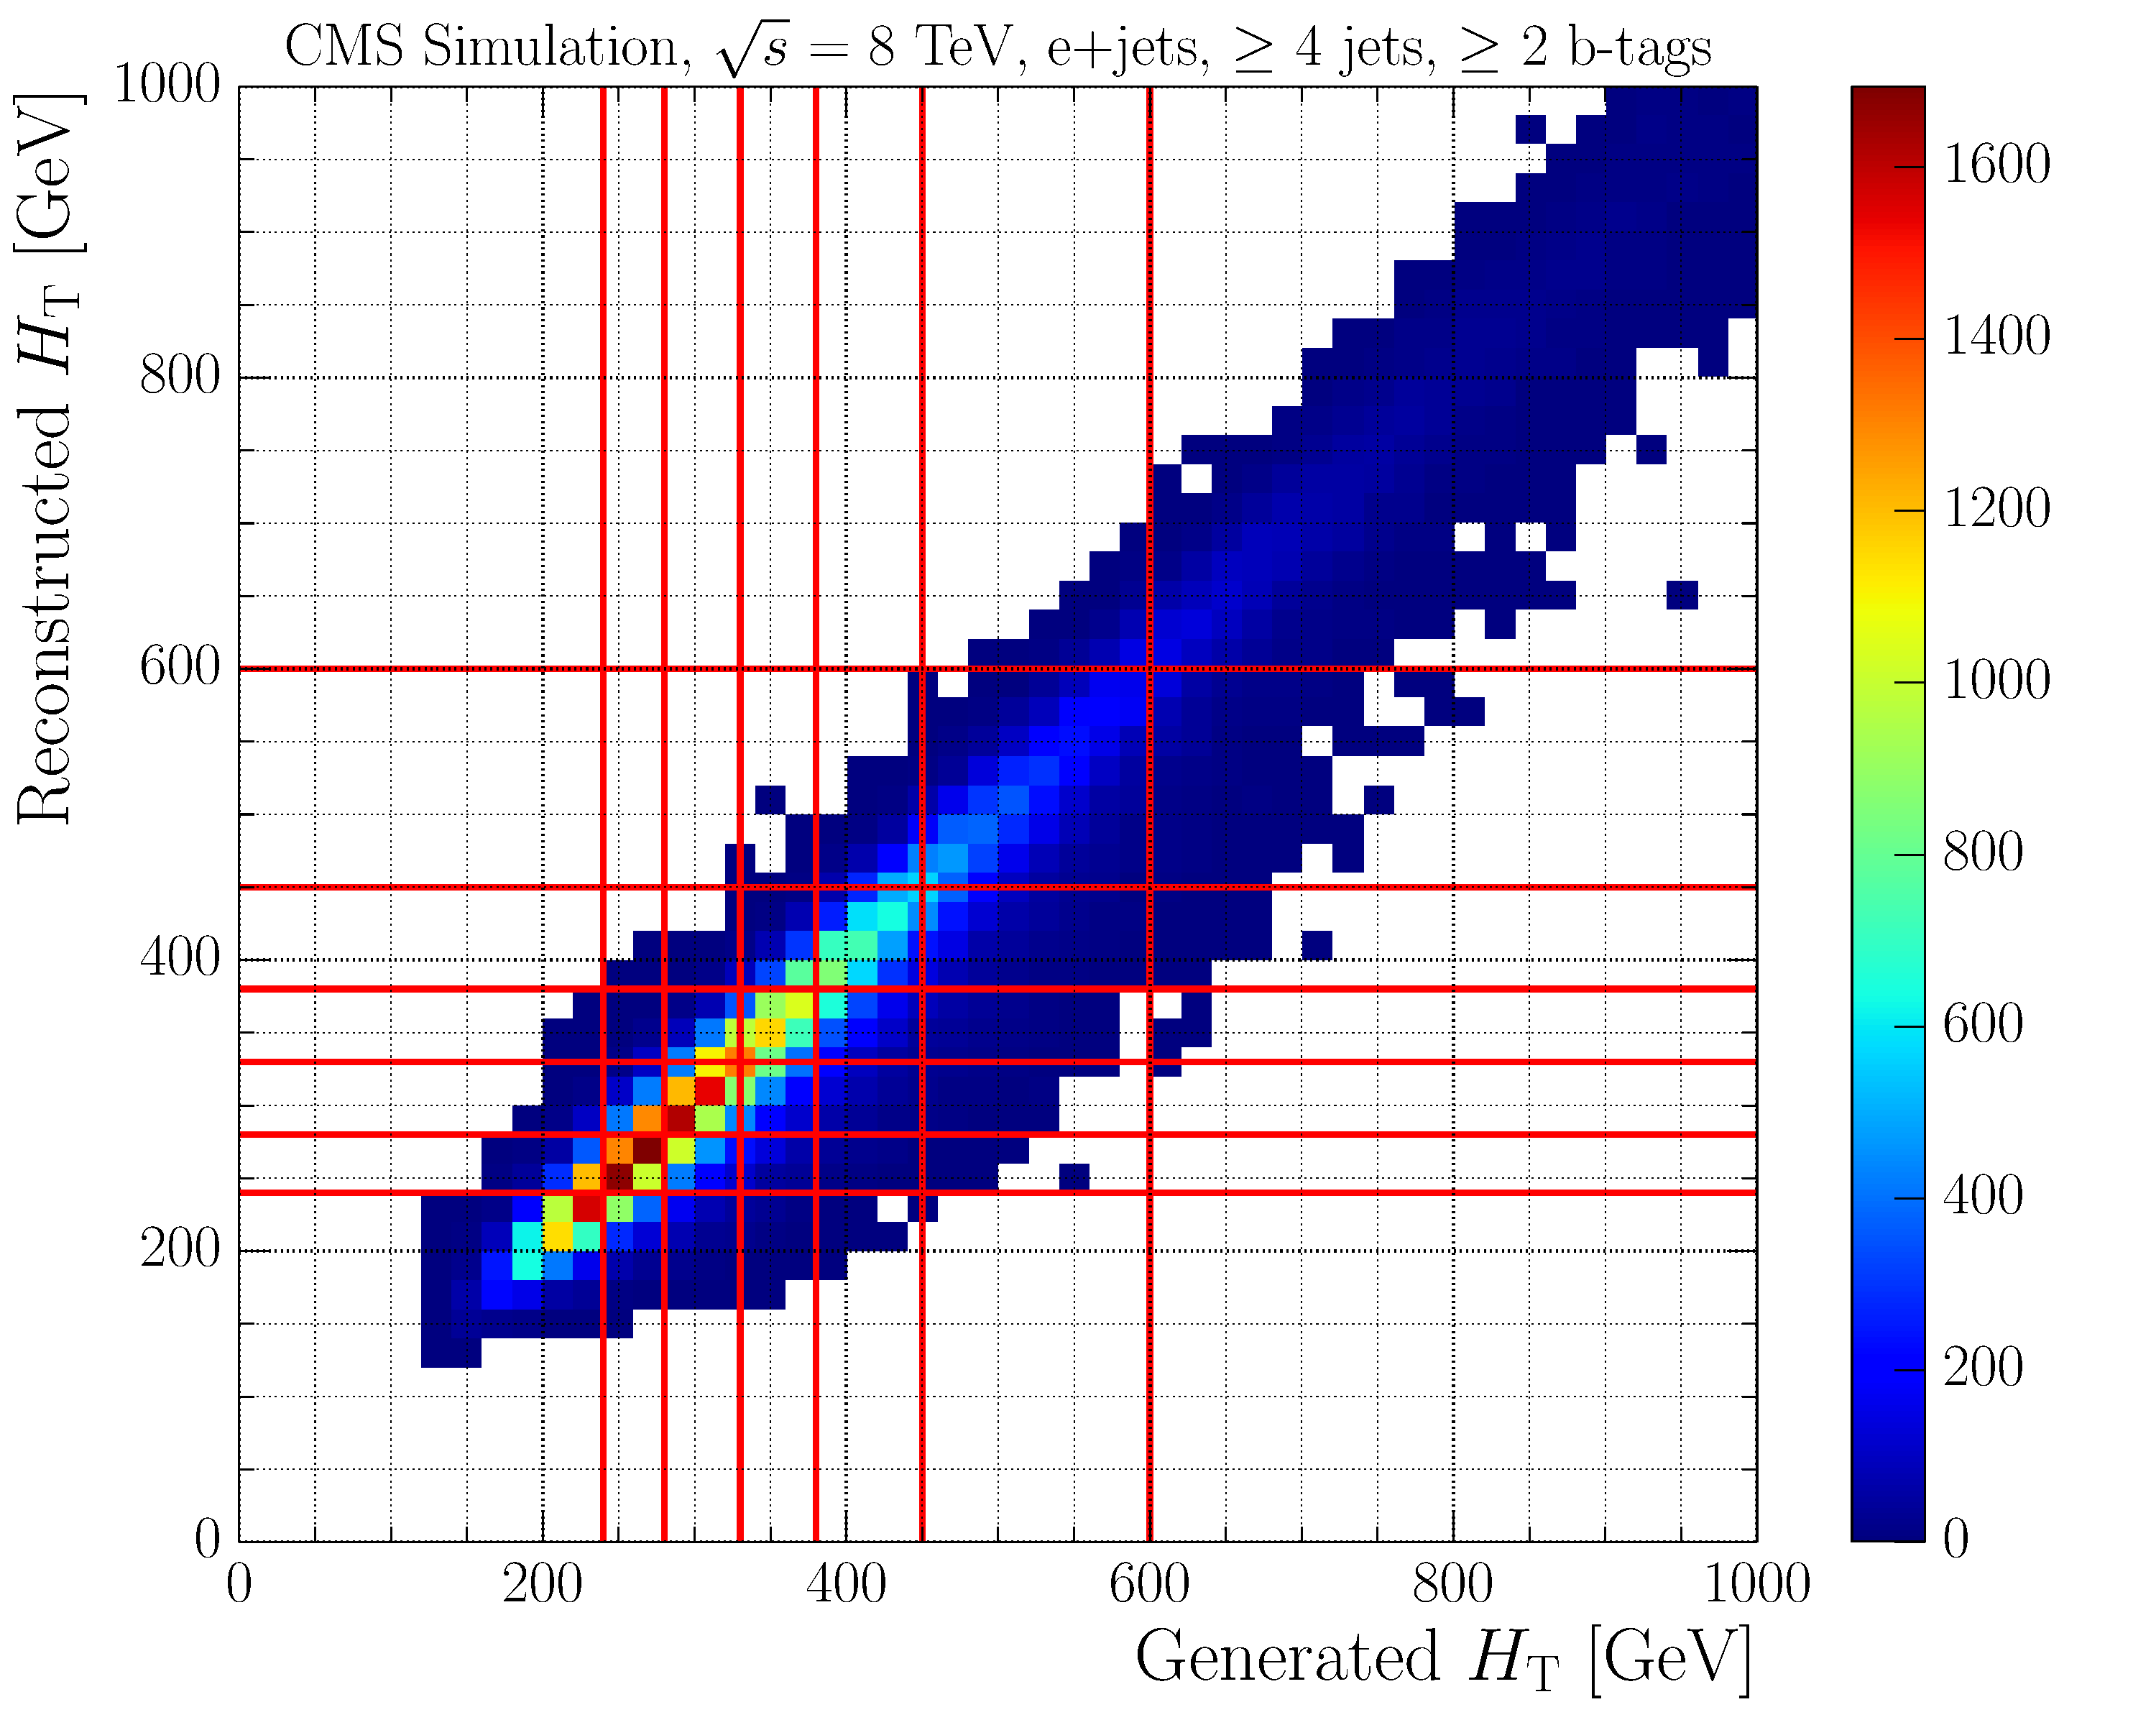
\includegraphics[width=0.5\textwidth]{binning/EPlusJets_HT}}\hfill
	\subfloat[]{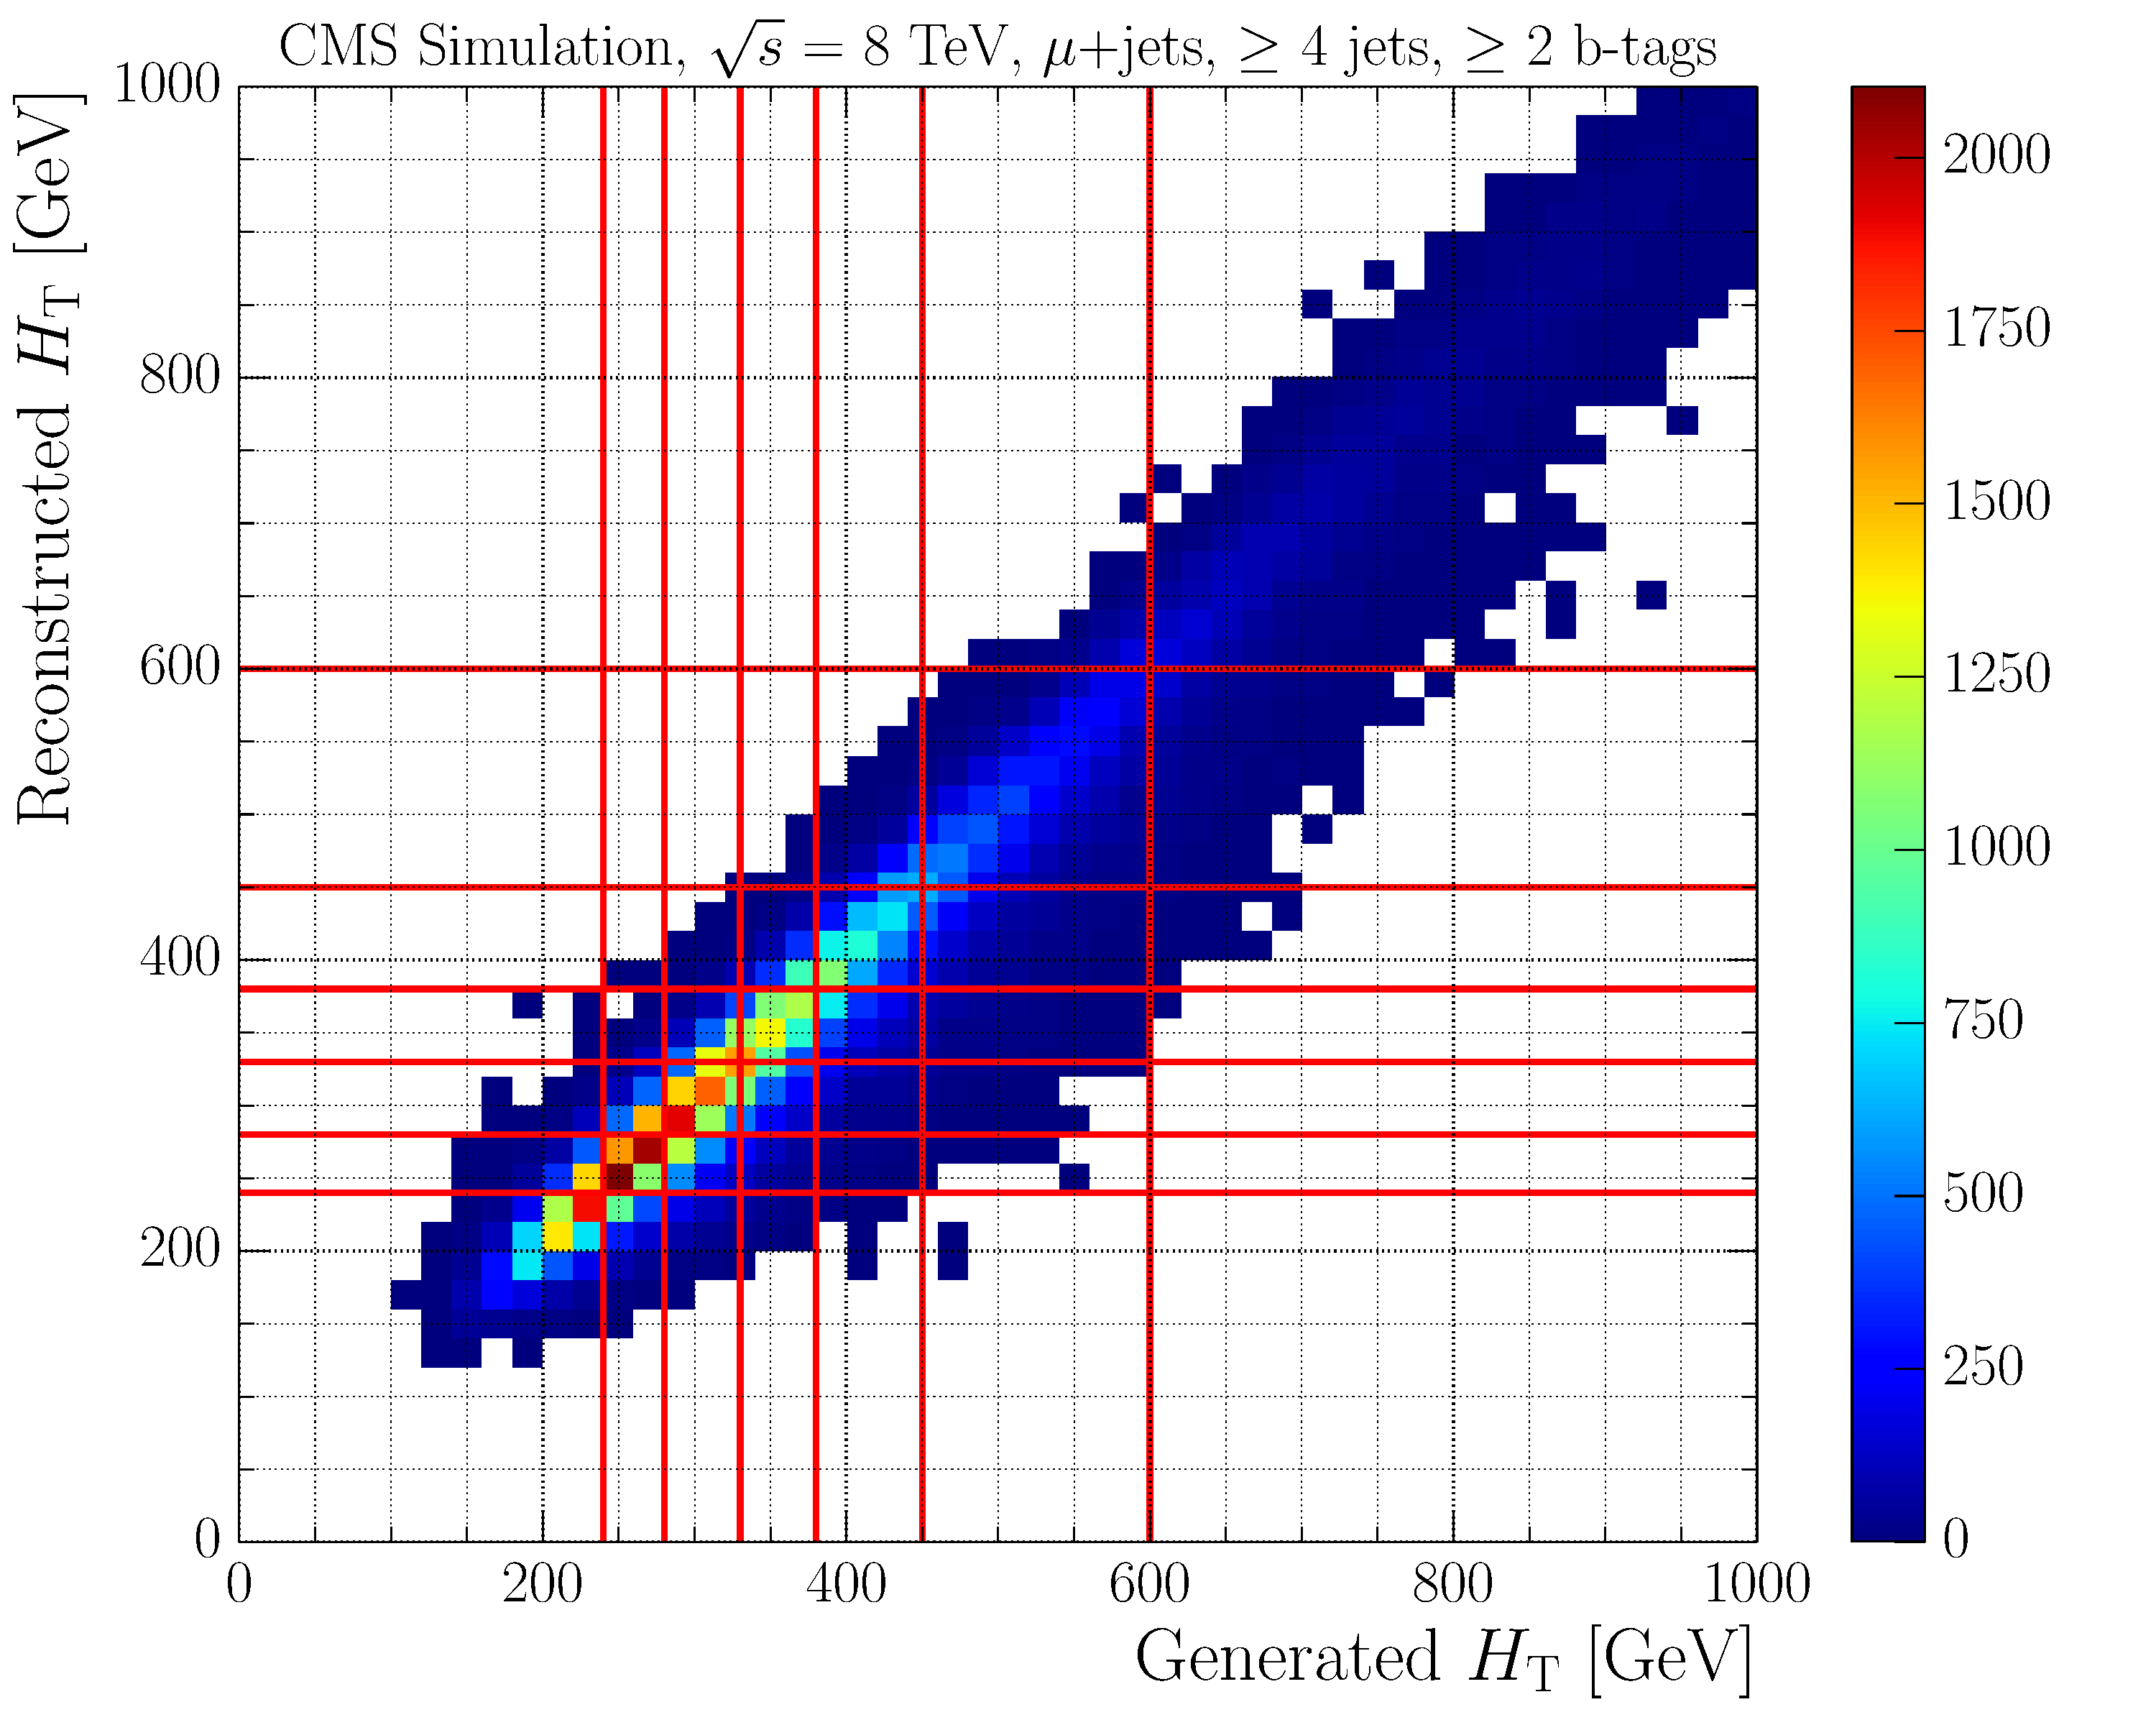
\includegraphics[width=0.5\textwidth]{binning/MuPlusJets_HT}}\\ 
	%ST
	\subfloat[]{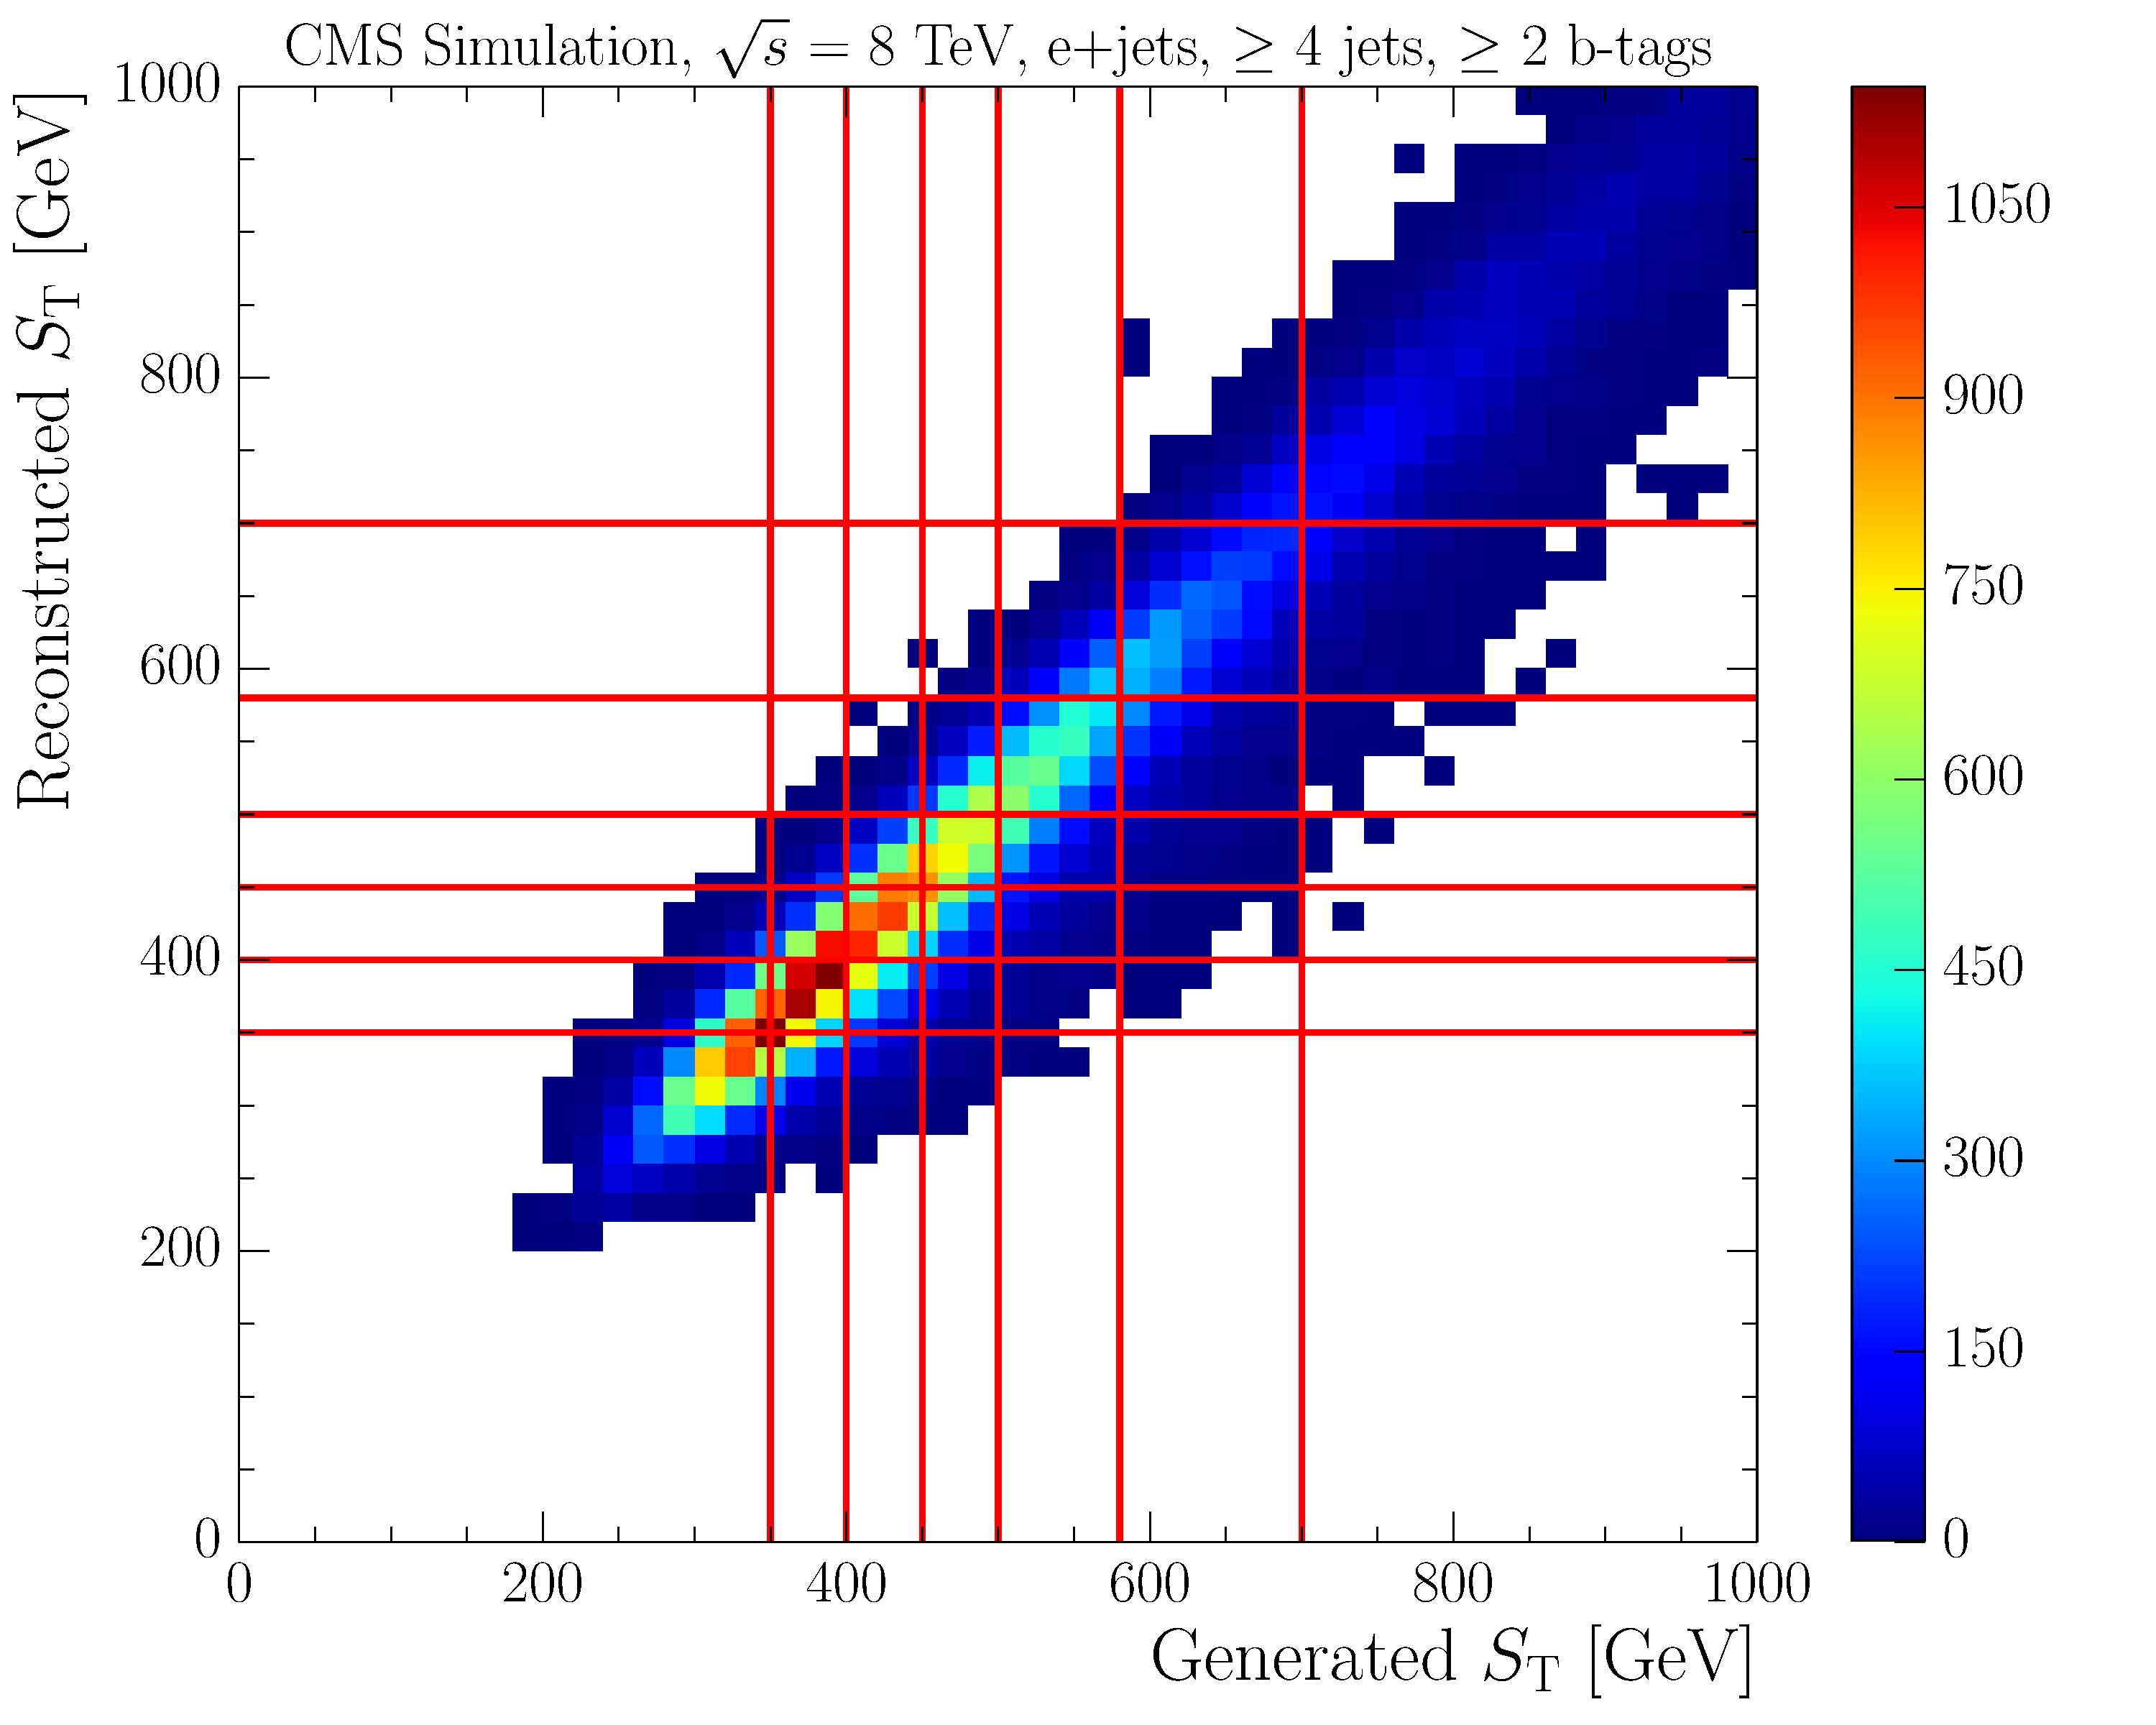
\includegraphics[width=0.5\textwidth]{binning/EPlusJets_ST}}\hfill
	\subfloat[]{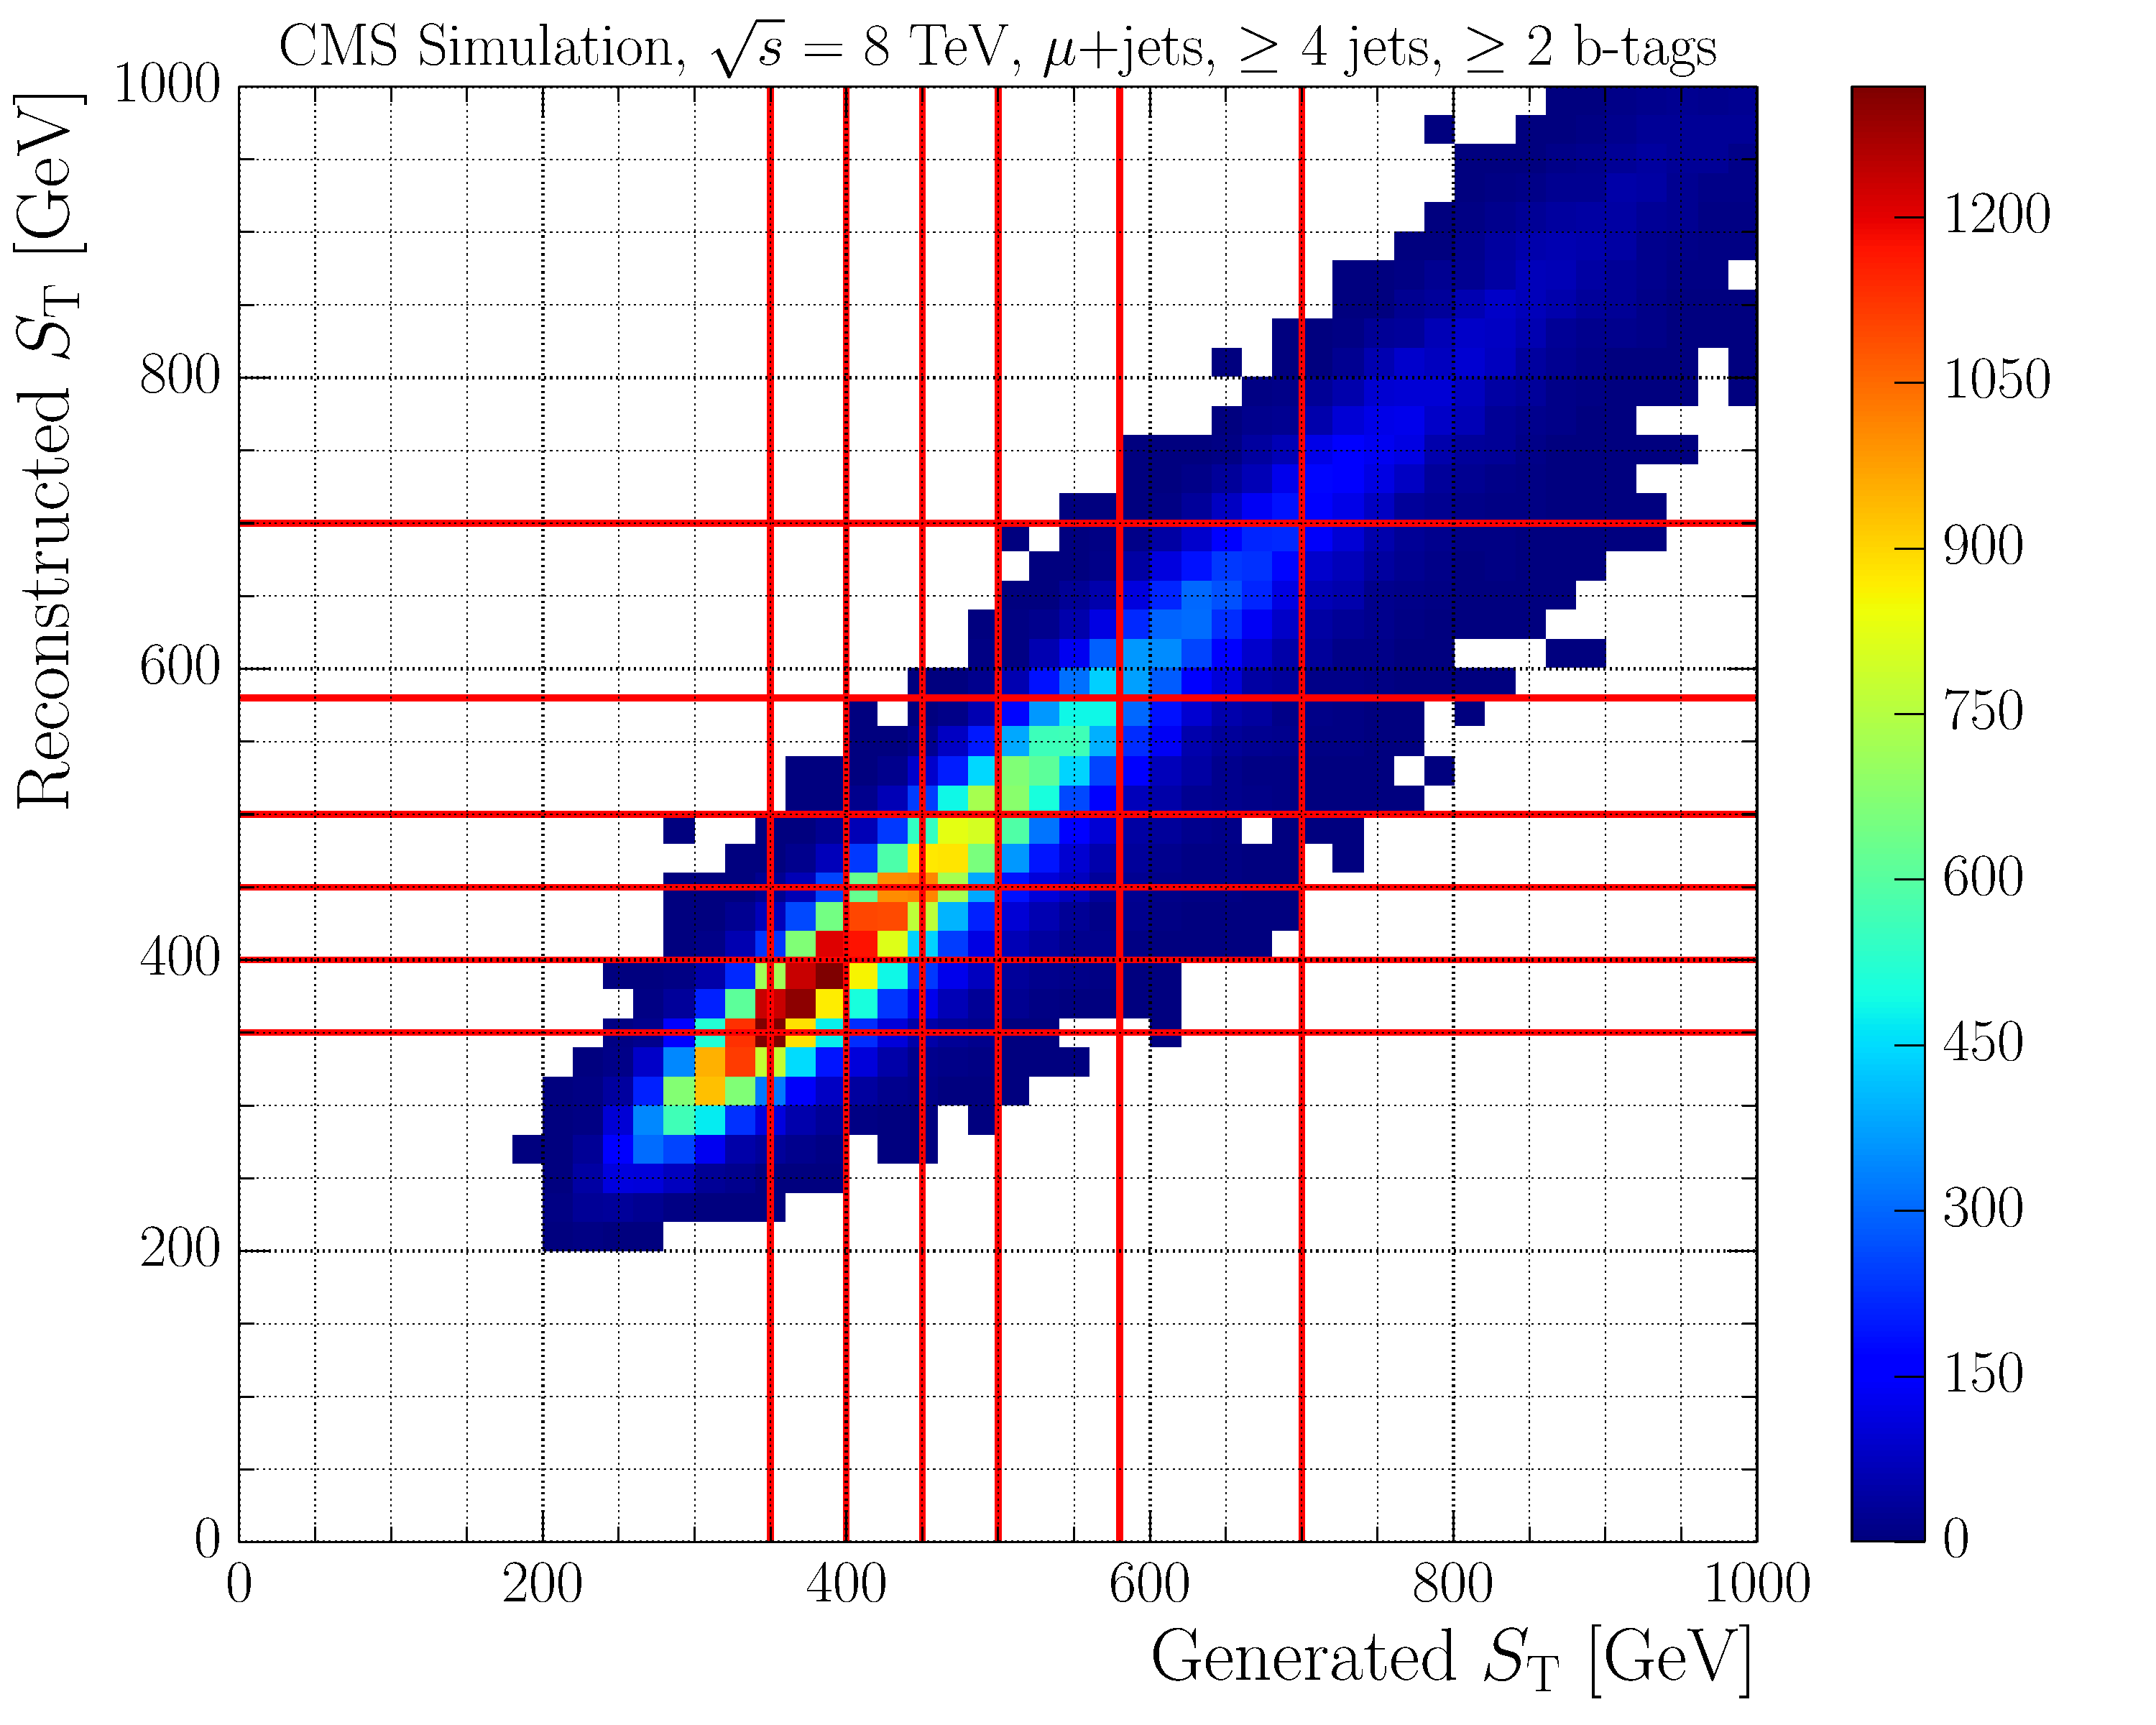
\includegraphics[width=0.5\textwidth]{binning/MuPlusJets_ST}}\\ 
	\caption{Reconstructed versus generated \HT (a, b) and \ST (c, d) for electron plus jets (left) and muon plus jets
	events (right).}
	\label{fig:choice_of_bins_appendix_1}
 \end{figure}

 \begin{figure}[hbtp]
	\centering
	%WPT
	\subfloat[]{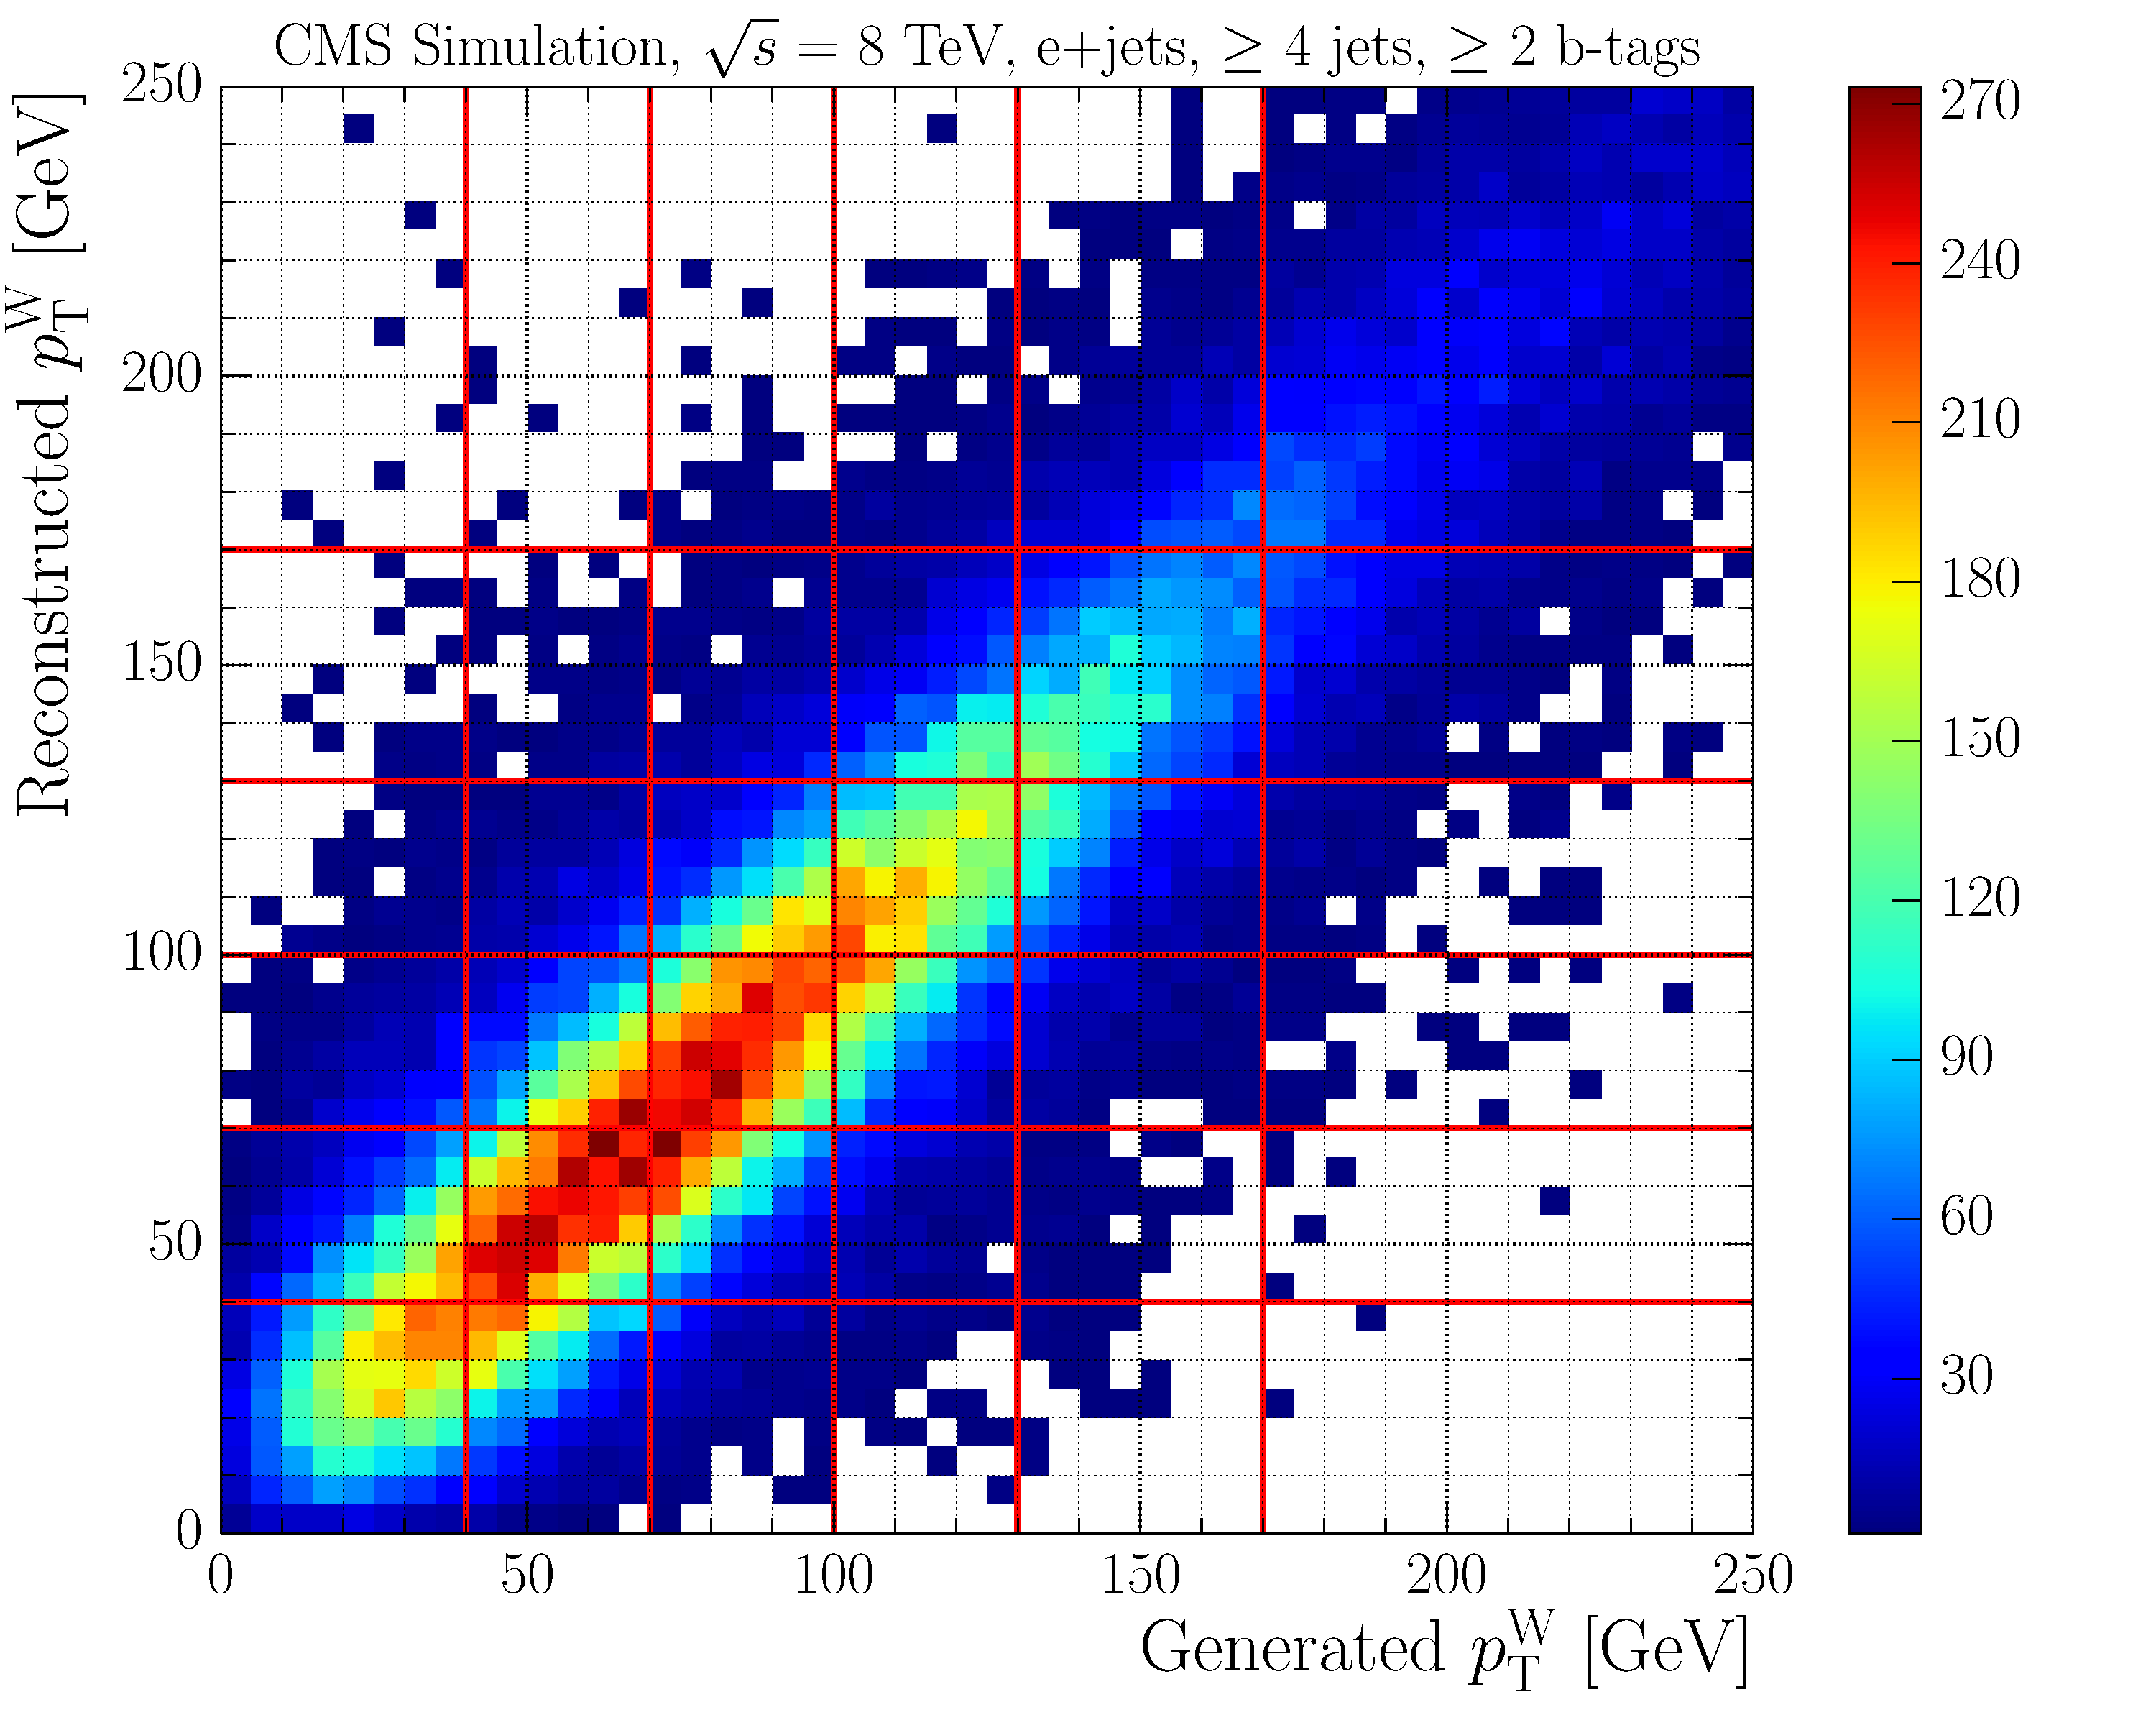
\includegraphics[width=0.5\textwidth]{binning/EPlusJets_WPT}}\hfill
	\subfloat[]{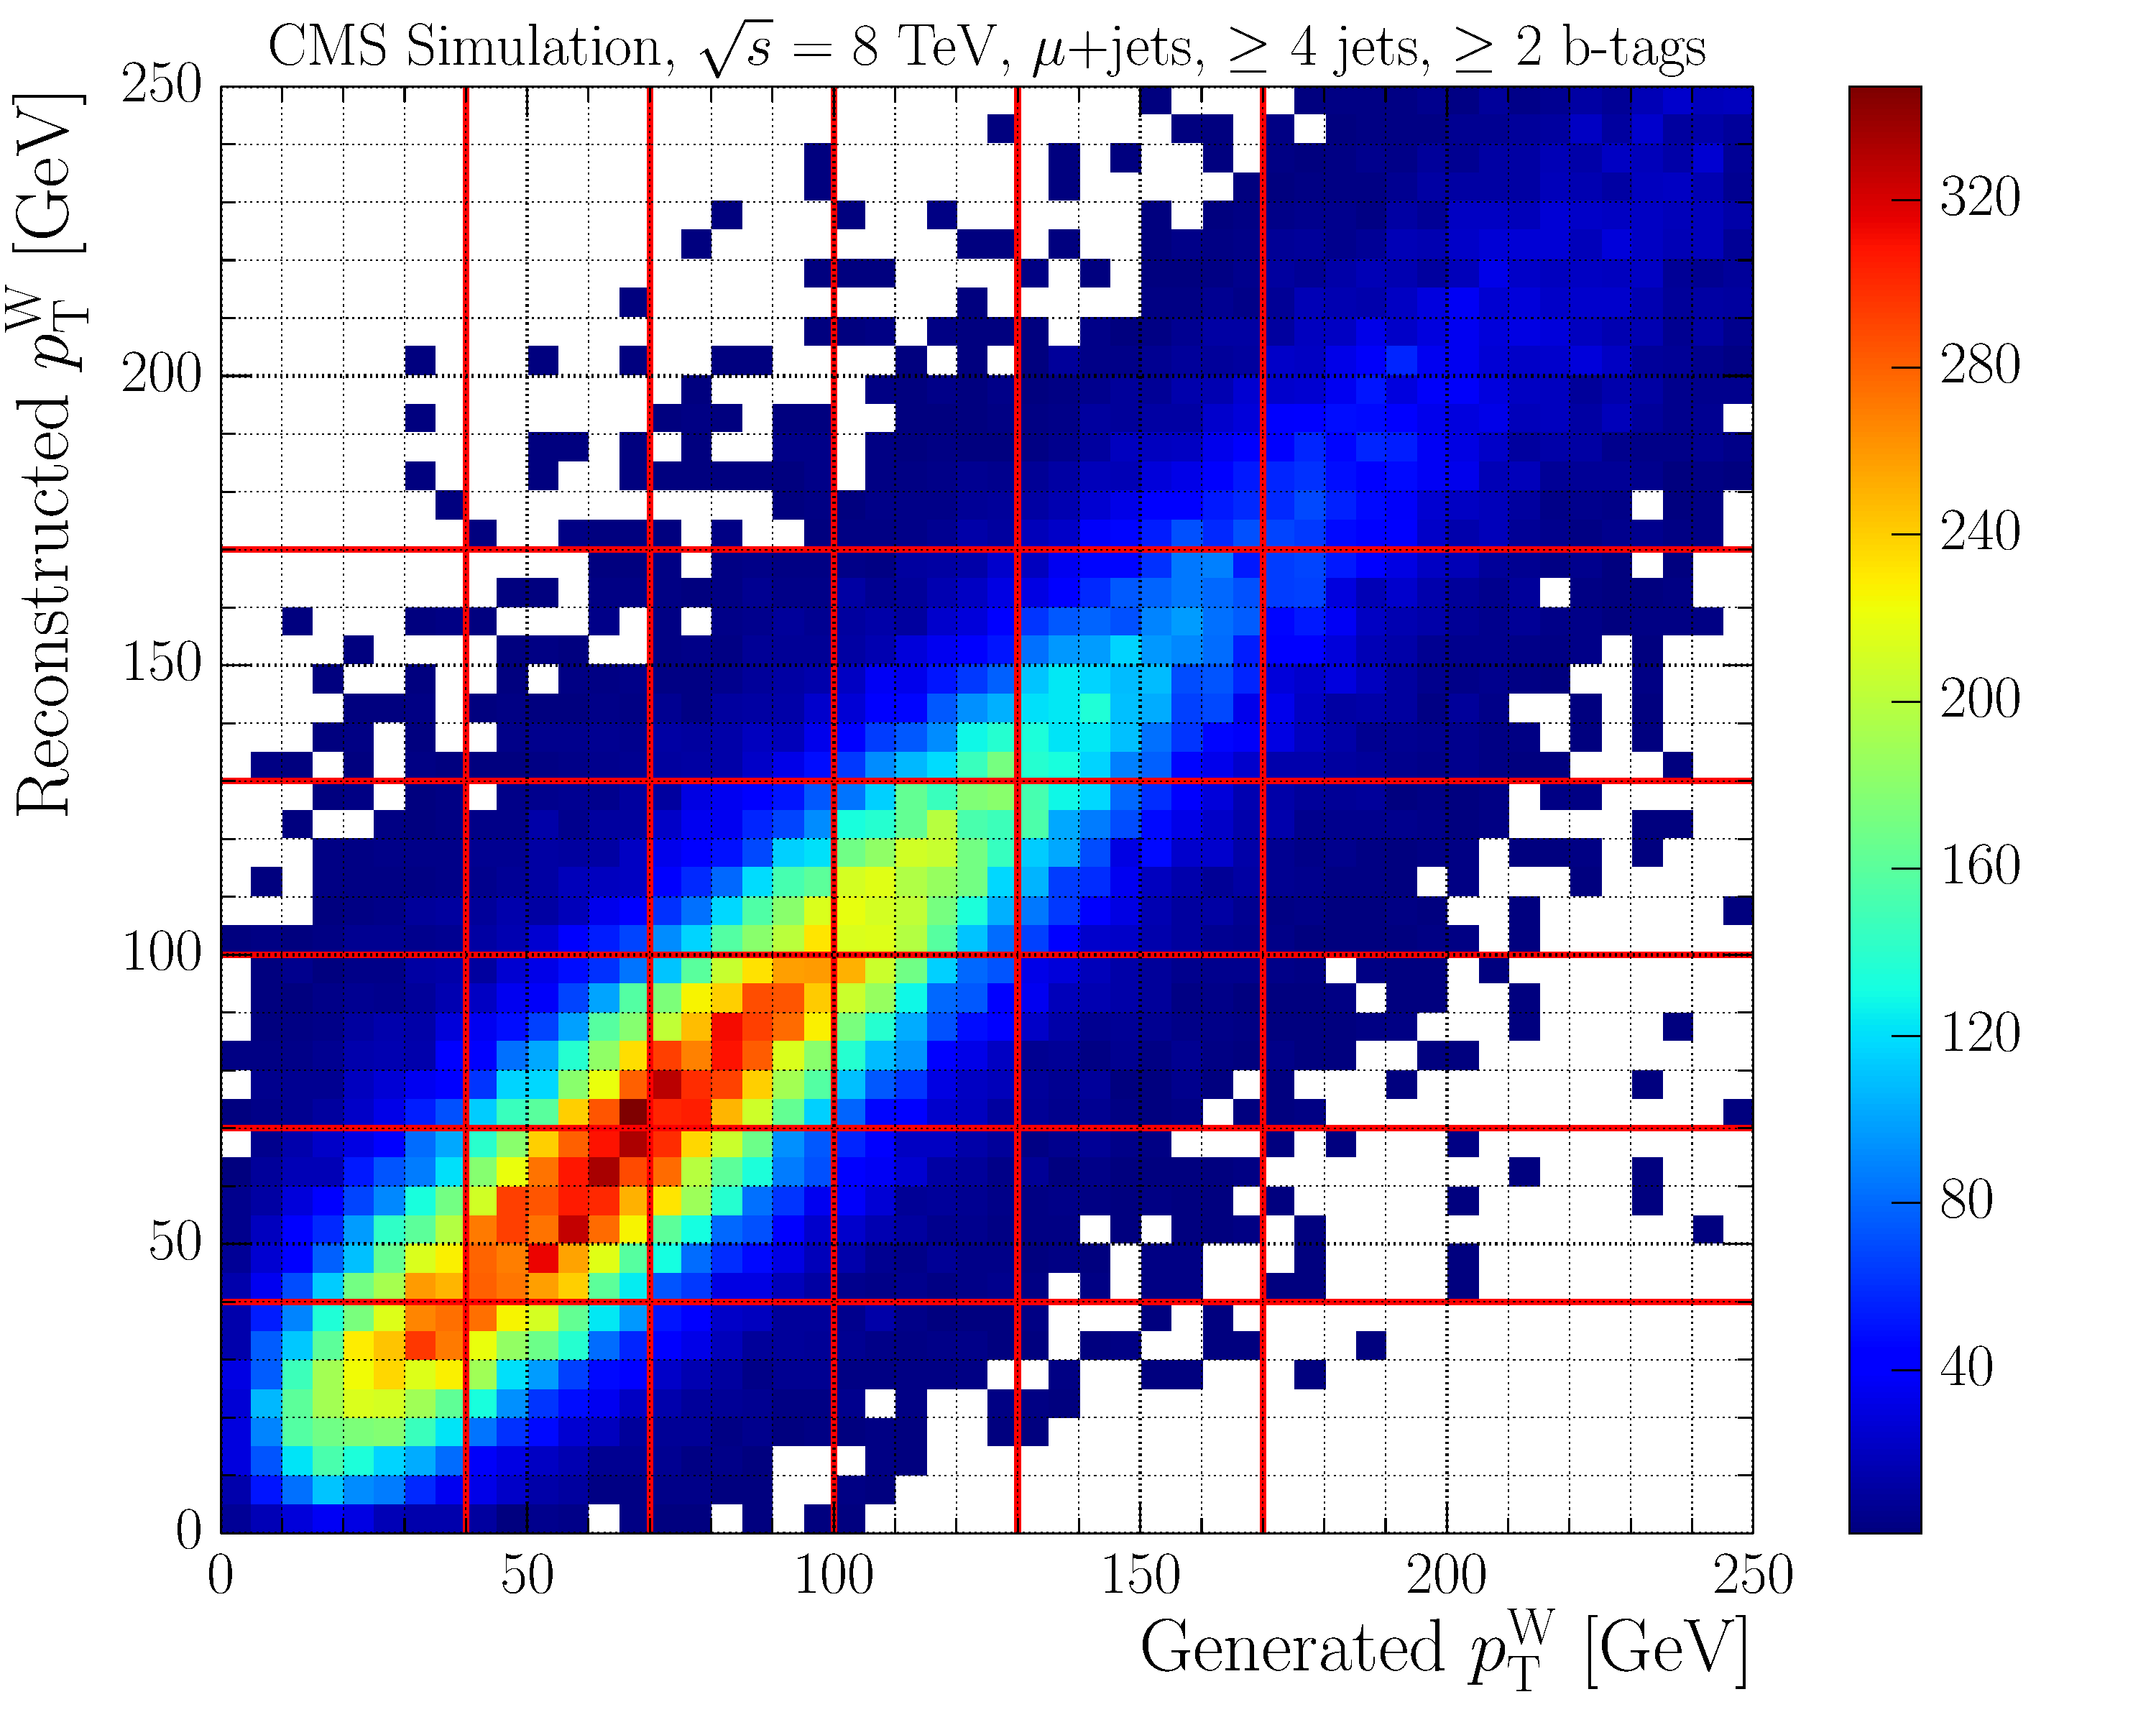
\includegraphics[width=0.5\textwidth]{binning/MuPlusJets_WPT}}\\
	%MT
	\subfloat[]{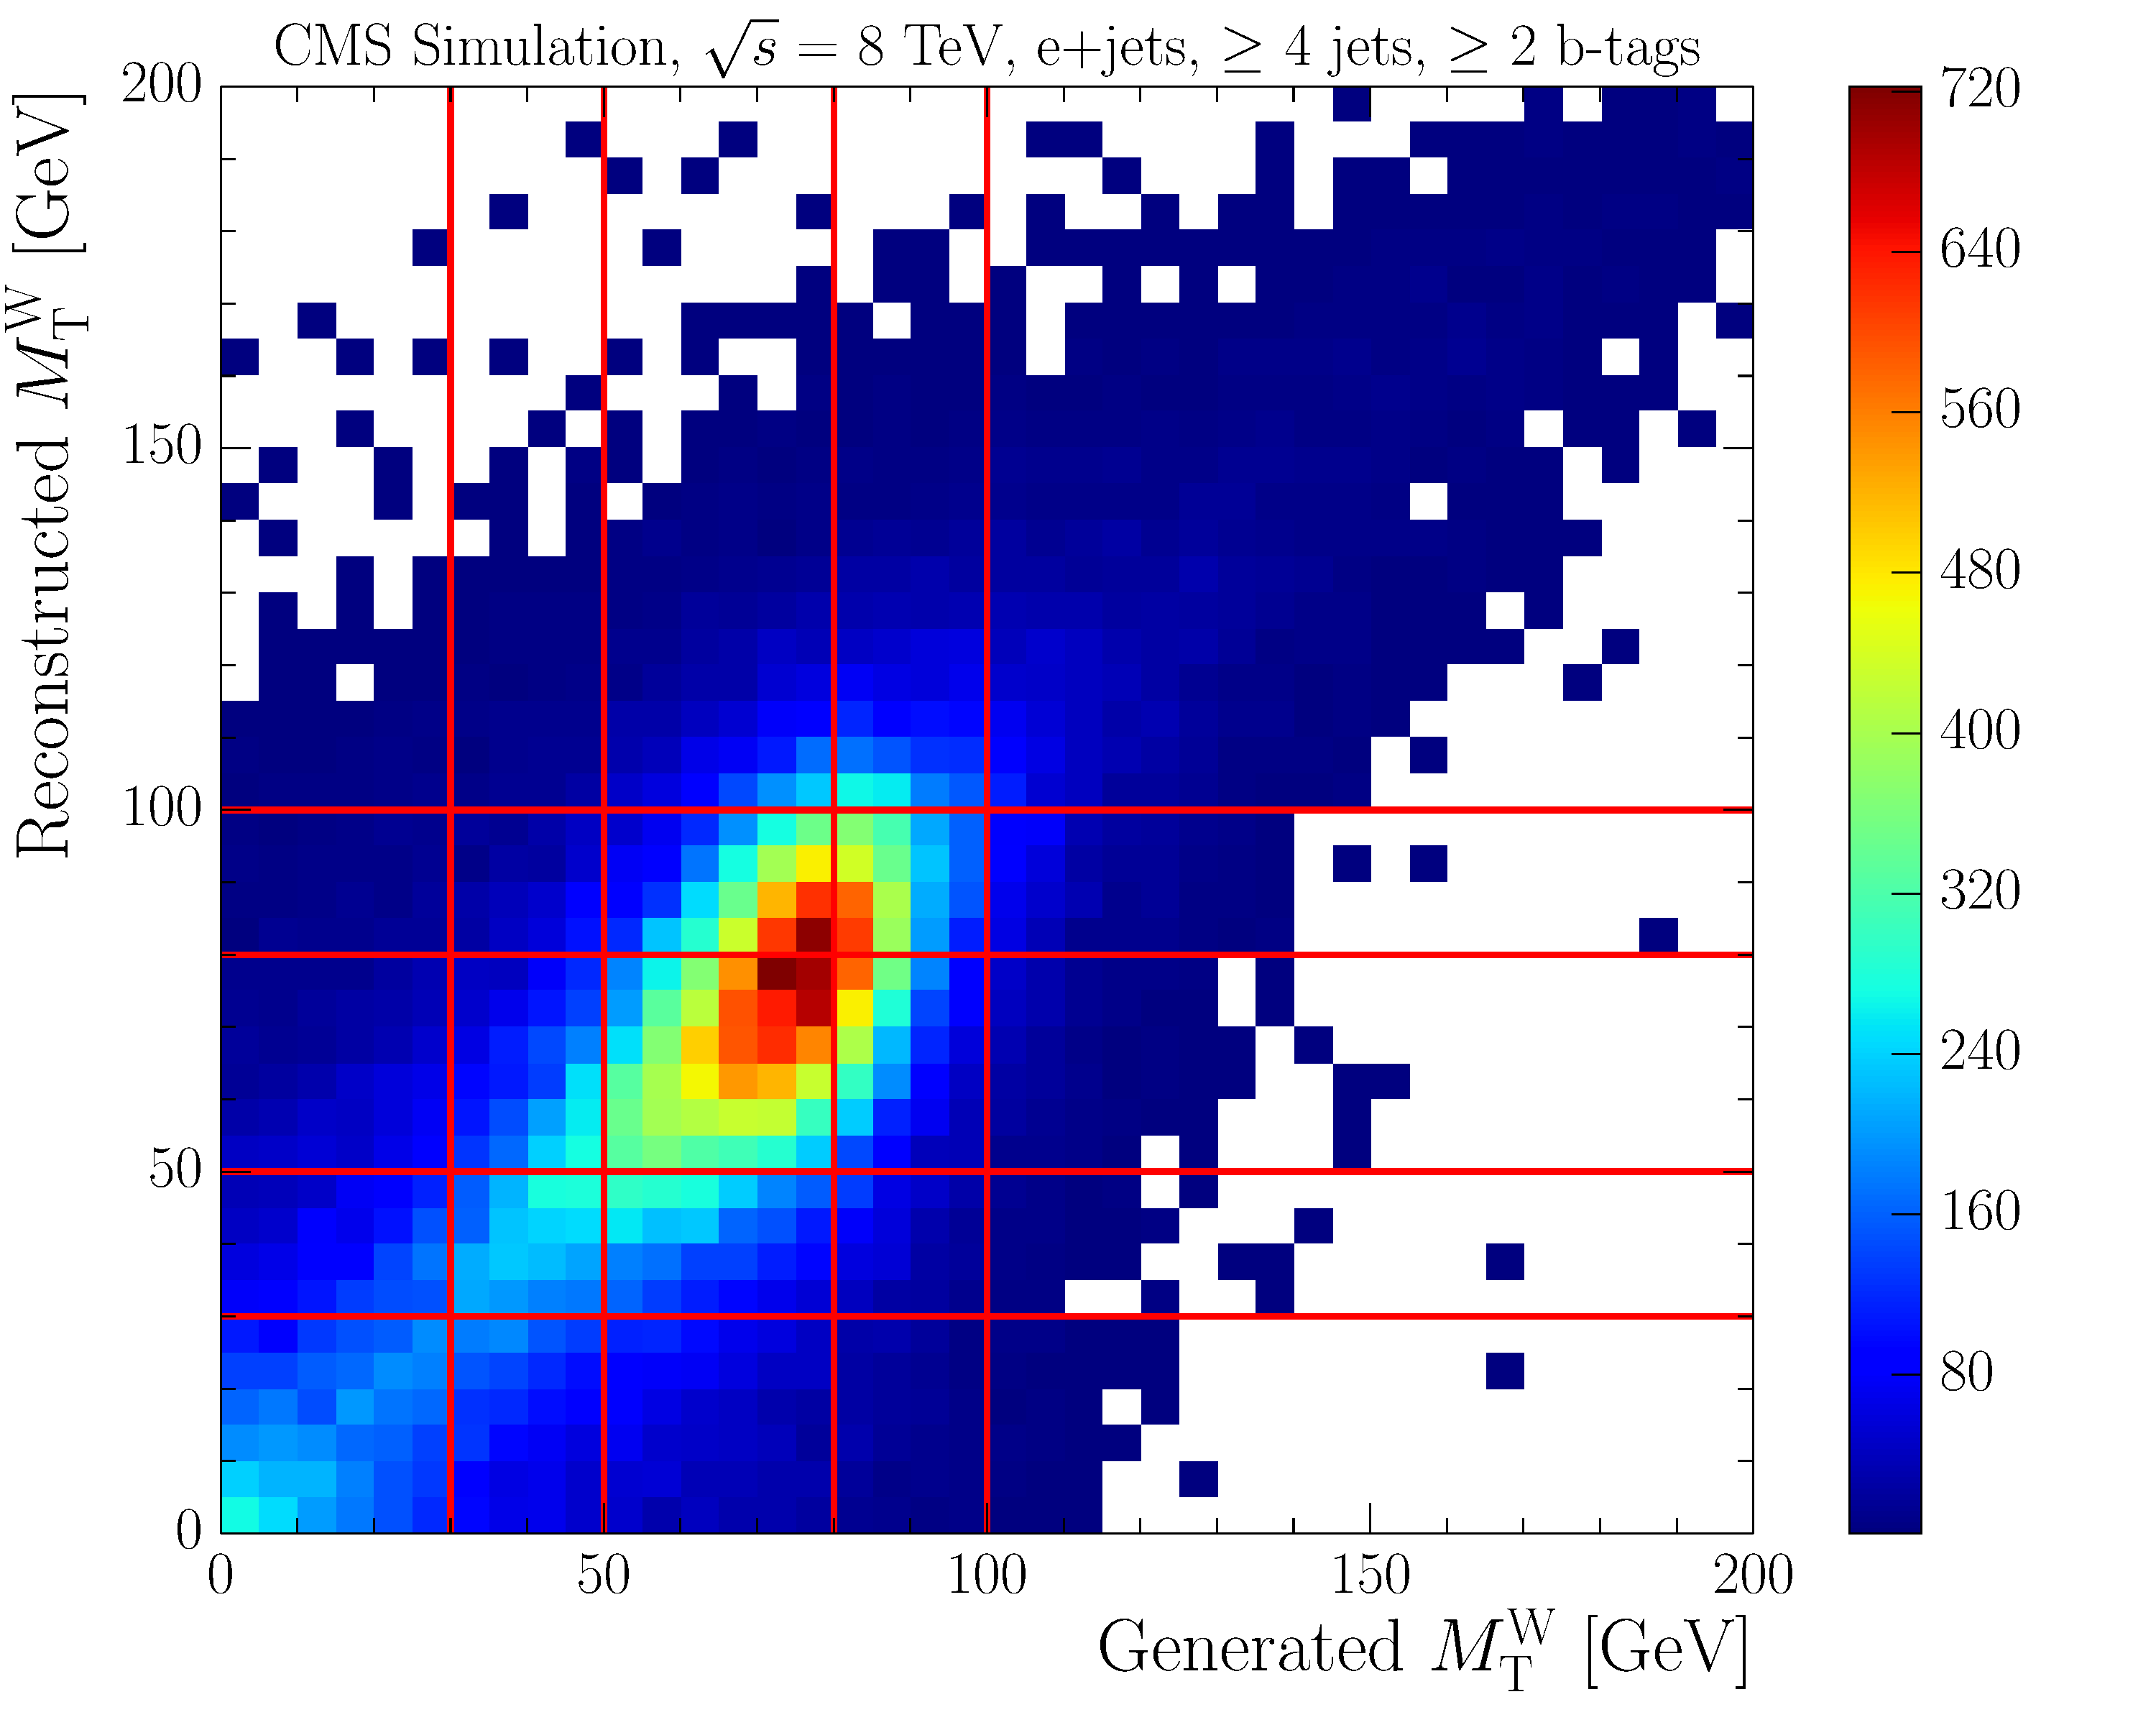
\includegraphics[width=0.5\textwidth]{binning/EPlusJets_MT}}\hfill
	\subfloat[]{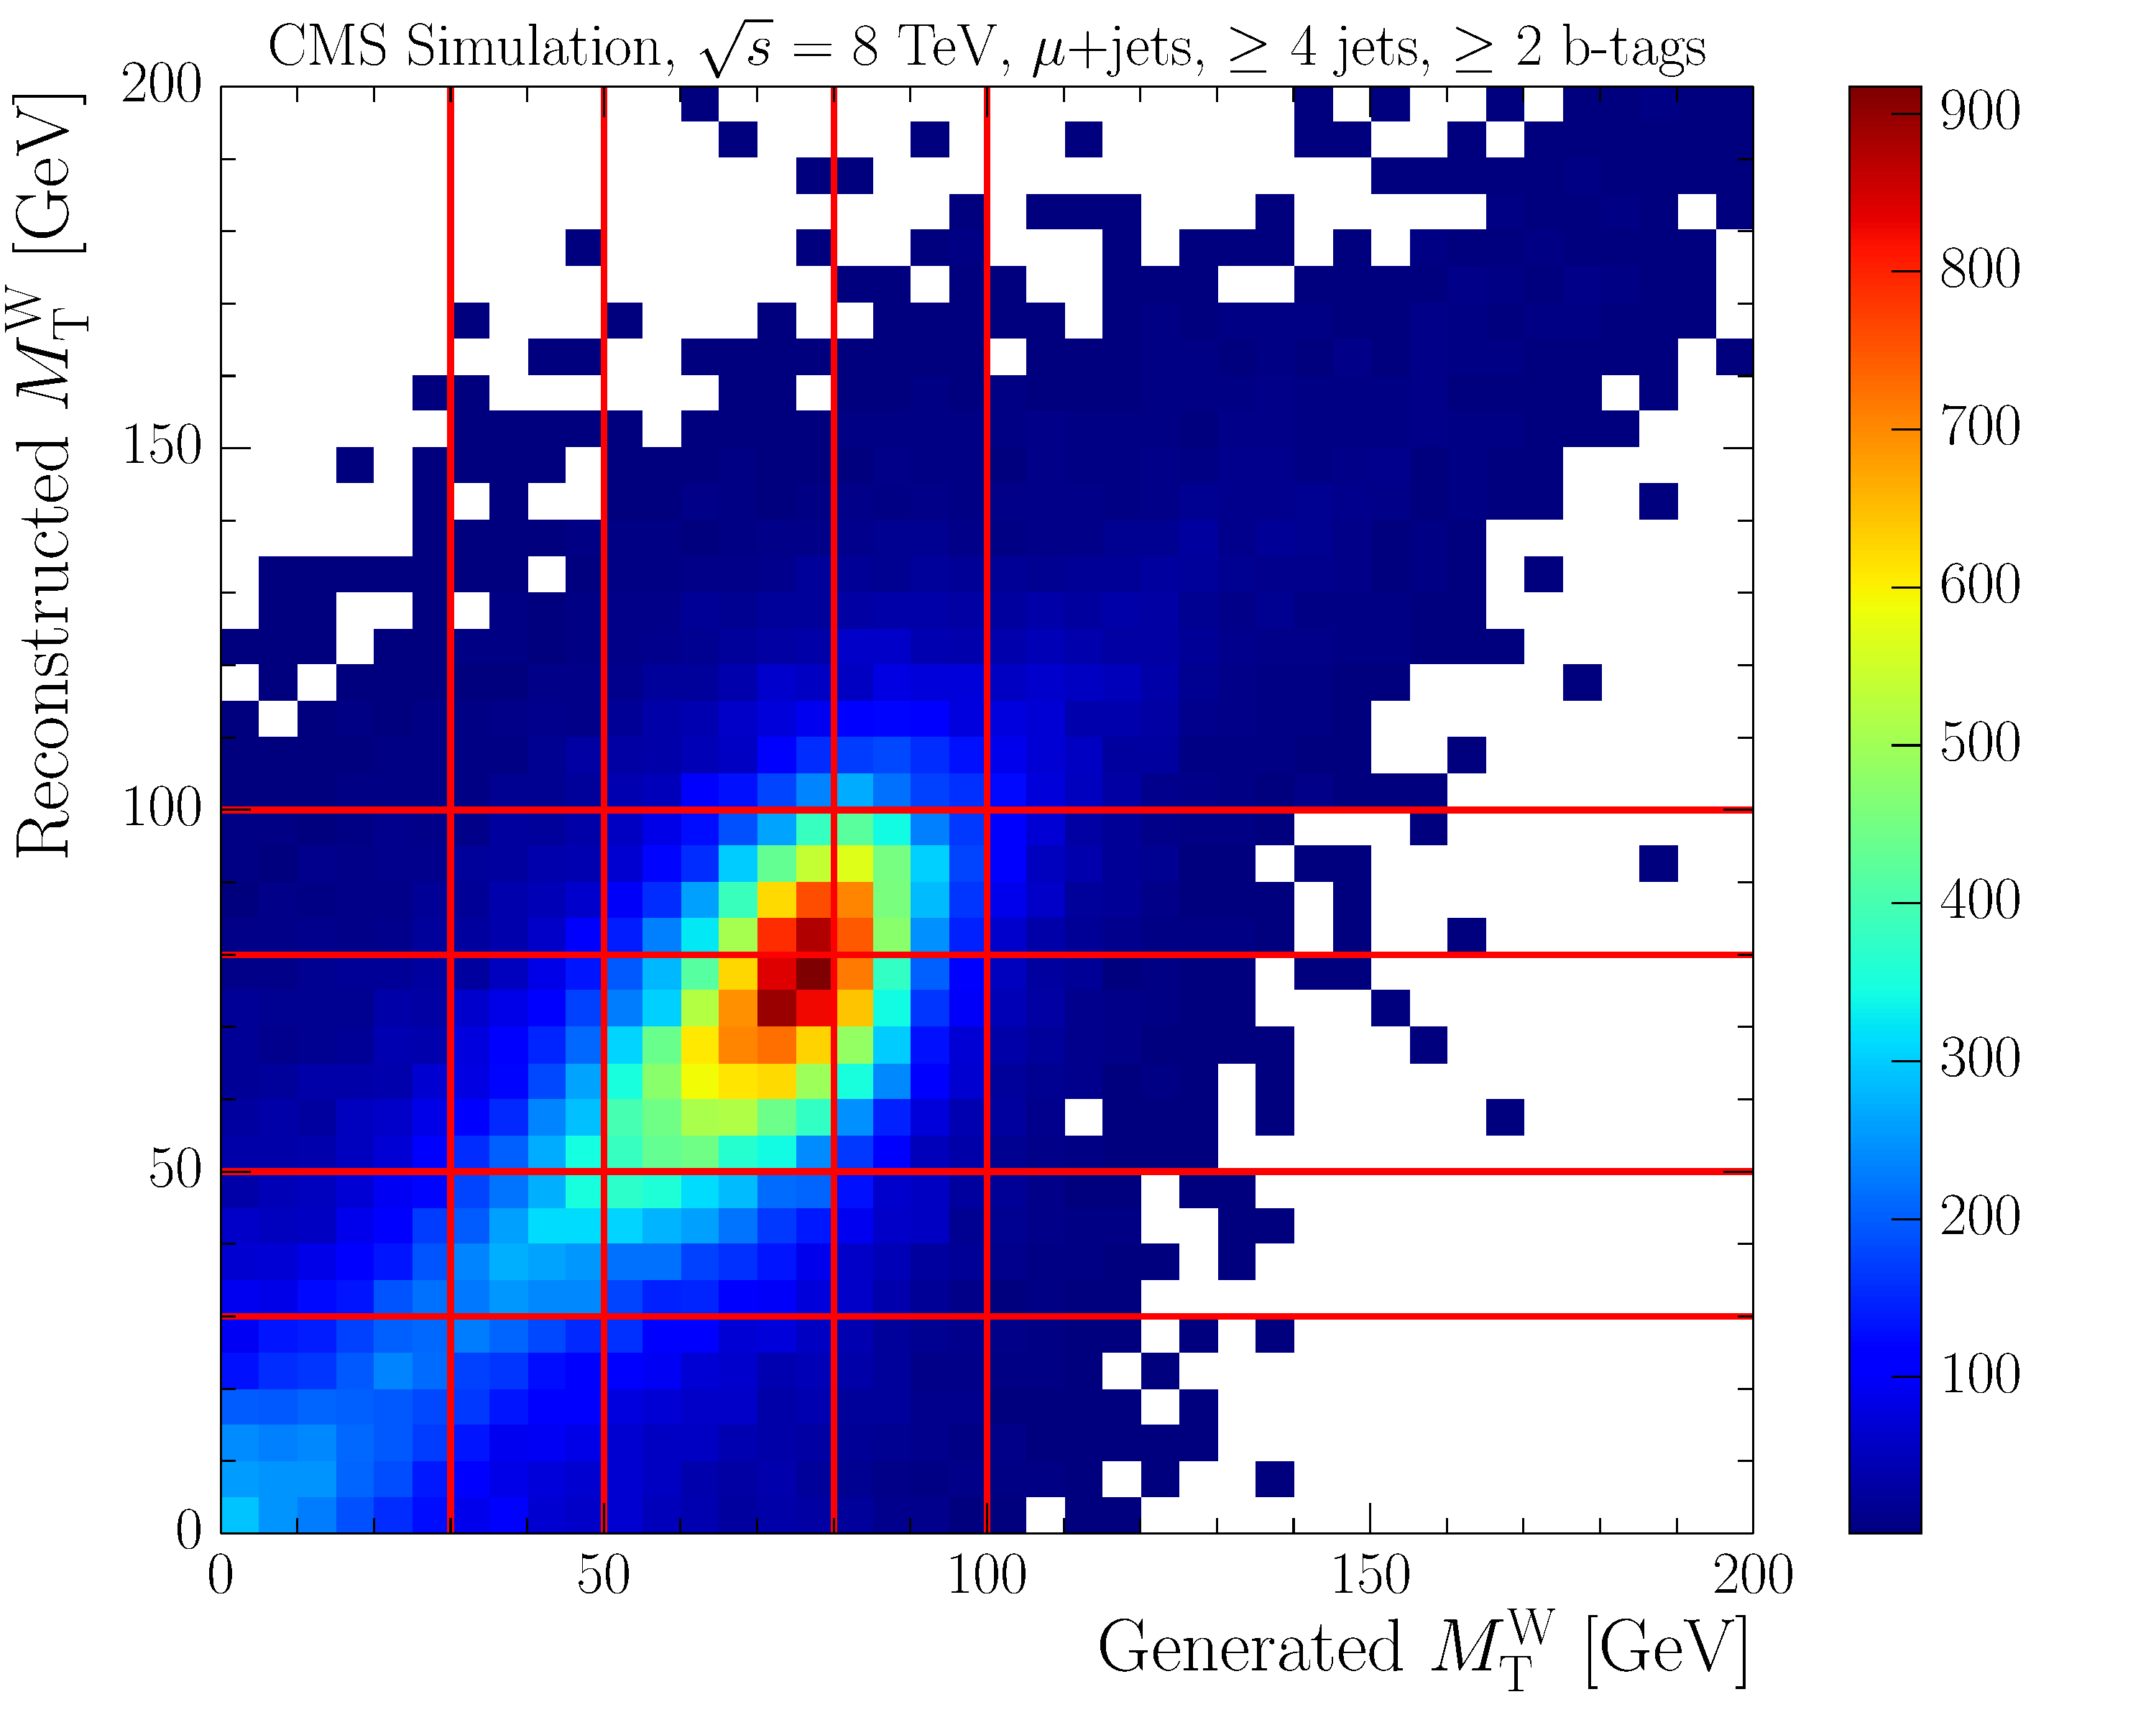
\includegraphics[width=0.5\textwidth]{binning/MuPlusJets_MT}}\\
	\caption{Reconstructed versus generated \WPT (a, b) and \MT (c, d) for electron plus jets (left) and muon plus jets
	events (right).}
	\label{fig:choice_of_bins_appendix_2}
 \end{figure}

\newpage


\begin{table}[htbp]
  	\centering
  	\caption{Stability and purity of chosen \HT bins in the electron channel for \ttbar MC events.}
  	\label{tab:binning_HT_electron}
	\resizebox{\columnwidth}{!}{
	\begin{tabular}{|l|r|r|r|r|r|r|r|}
	\toprule
	bin & $80 < \HT < 240$ & $240 \leq \HT <280$ & $280 \leq \HT < 330$ & $330 \leq \HT < 380$ & $380 \leq \HT < 450$ & $450 \leq \HT < 600$ & $\HT \geq 600$ \\
	\midrule 
	events & 10601 & 12569 & 14372 & 12397 & 10893 & 10721 & 5609\\
	purity & 0.82 & 0.62 & 0.63 & 0.62 & 0.68 & 0.81 & 0.9\\
	stability &  0.76 & 0.63 & 0.65 & 0.64 & 0.68 & 0.8 & 0.9\\
	\bottomrule
	\end{tabular}
	}
\end{table}


\begin{table}[htbp]
  	\centering
  	\caption{Stability and purity of chosen \HT bins in the muon channel for \ttbar MC events.}
  	\label{tab:binning_HT_muon}
	\resizebox{\columnwidth}{!}{
	\begin{tabular}{|l|r|r|r|r|r|r|r|}
	\toprule
	bin & $80 < \HT < 240$ & $240 \leq \HT <280$ & $280 \leq \HT < 330$ & $330 \leq \HT < 380$ & $380 \leq \HT < 450$ & $450 \leq \HT < 600$ & $\HT \geq 600$ \\
	\midrule 
	events & 12337 & 14821 & 16747 & 14268 & 12258 & 12119 & 5857\\
	purity & 0.82 & 0.63 & 0.64 & 0.63 & 0.67 & 0.81 & 0.9\\
	stability & 0.76 & 0.64 & 0.65 & 0.65 & 0.68 & 0.81 & 0.89\\
	\bottomrule
	\end{tabular}
	}
\end{table}



\begin{table}[htbp]
  	\centering
  	\caption{Stability and purity of chosen \ST bins in the electron channel for \ttbar MC events.}
  	\label{tab:binning_ST_electron}
	\resizebox{\columnwidth}{!}{
	\begin{tabular}{|l|r|r|r|r|r|r|r|}
	\toprule
	bin & $106 < \ST < 350$ & $ 350 \leq \ST < 400$ & $400 \leq \ST < 450$ & $450 \leq \ST < 500$ & $500 \leq \ST < 580$ & $580 \leq \ST < 700$ & $\ST \geq 700$ \\
	\midrule 
	events & 11183 & 13246 & 12073 & 10709 & 11317 & 9166 & 8373\\
	purity & 0.83 & 0.6 & 0.53 & 0.53 & 0.63 & 0.71 & 0.87\\
	stability & 0.73 & 0.6 & 0.55 & 0.55 & 0.66 & 0.73 & 0.91\\ 
	\bottomrule
	\end{tabular}
	}
\end{table}


\begin{table}[htbp]
  	\centering
  	\caption{Stability and purity of chosen \ST bins in the muon channel for \ttbar MC events.}
  	\label{tab:binning_ST_muon}
	\resizebox{\columnwidth}{!}{
	\begin{tabular}{|l|r|r|r|r|r|r|r|}
	\toprule
	bin & $106 < \ST < 350$ & $ 350 \leq \ST < 400$ & $400 \leq \ST < 450$ & $450 \leq \ST < 500$ & $500 \leq \ST < 580$ & $580 \leq \ST < 700$ & $\ST \geq 700$ \\
	\midrule 
	events & 13593 & 15717 & 13878 & 12307 & 12732 & 10135 & 8875\\
	purity &  0.83 & 0.61 & 0.54 & 0.54 & 0.64 & 0.71 & 0.87\\
	stability & 0.74 & 0.61 & 0.55 & 0.56 & 0.66 & 0.74 & 0.9\\
	\bottomrule
	\end{tabular}
	}
\end{table}


\begin{table}[htbp]
  	\centering
  	\caption{Stability and purity of chosen \WPT bins in the electron channel for \ttbar MC events.}
  	\label{tab:binning_WPT_electron}
	\resizebox{\columnwidth}{!}{
	\begin{tabular}{|l|r|r|r|r|r|r|}
	\toprule
	bin & $0 < \WPT < 40$ & $40 \leq \WPT < 70$ & $70 \leq \WPT < 100$ & $100 \leq \WPT < 130$ & $130 \leq \WPT < 170$ & $\WPT \geq 170$ \\
	\midrule 
	events &  10005 & 15849 & 16053 & 12203 & 9532 & 7717\\
	purity & 0.64 & 0.54 & 0.52 & 0.5 & 0.56 & 0.77\\
	stability & 0.63 & 0.54 & 0.52 & 0.51 & 0.57 & 0.76\\
	\bottomrule
	\end{tabular}
	}
\end{table}


\begin{table}[htbp]
  	\centering
  	\caption{Stability and purity of chosen \WPT bins in the muon channel for \ttbar MC events.}
  	\label{tab:binning_WPT_muon}
	\resizebox{\columnwidth}{!}{
	\begin{tabular}{|l|r|r|r|r|r|r|}
	\toprule
	bin & $0 < \WPT < 40$ & $40 \leq \WPT < 70$ & $70 \leq \WPT < 100$ & $100 \leq \WPT < 130$ & $130 \leq \WPT < 170$ & $\WPT \geq 170$ \\
	\midrule 
	events &  12379 & 18821 & 18330 & 13495 & 10260 & 8394 \\
	purity & 0.67 & 0.55 & 0.52 & 0.5 & 0.55 & 0.76\\
	stability & 0.63 & 0.55 & 0.53 & 0.51 & 0.56 & 0.76\\
	\bottomrule
	\end{tabular}
	}
\end{table}


\begin{table}[htbp]
  	\centering
  	\caption{Stability and purity of chosen \MT bins in the electron channel for \ttbar MC events.}
  	\label{tab:binning_MT_electron}
	\resizebox{\columnwidth}{!}{
	\begin{tabular}{|l|r|r|r|r|r|}
	\toprule
	bin & $0 < \MT < 30$ & $30 \leq \MT < 50$ & $50 \leq \MT < 80$ & $80 \leq \MT < 100$ & $MT \geq 100$ \\
	\midrule 
	events &  11509 & 11633 & 26288 & 14824 & 8921 \\
	purity & 0.57 & 0.35 & 0.65 & 0.4 & 0.36\\
	stability & 0.62 & 0.37 & 0.53 & 0.41 & 0.67\\
	\bottomrule
	\end{tabular}
	}
\end{table}


\begin{table}[htbp]
  	\centering
  	\caption{Stability and purity of chosen \MT bins in the muon channel for \ttbar MC events.}
  	\label{tab:binning_MT_muon}
	\resizebox{\columnwidth}{!}{
	\begin{tabular}{|l|r|r|r|r|r|}
	\toprule
	bin & $0 < \MT < 30$ & $30 \leq \MT < 50$ & $50 \leq \MT < 80$ & $80 \leq \MT < 100$ & $MT \geq 100$ \\
	\midrule 
	events & 13209 & 13636 & 30669 & 16974 & 9179.3\\
	purity & 0.56 & 0.36 & 0.66 & 0.42 & 0.37\\
	stability & 0.64 & 0.38 & 0.54 & 0.42 & 0.66\\
	\bottomrule
	\end{tabular}
	}
\end{table}

\chapter{Fitting templates}
\label{a:templates}

\sisetup{range-phrase = --}
\sisetup{range-units = single}

%%% MET %%%

% \begin{figure}[!htbp]
% 	\centering
%   	{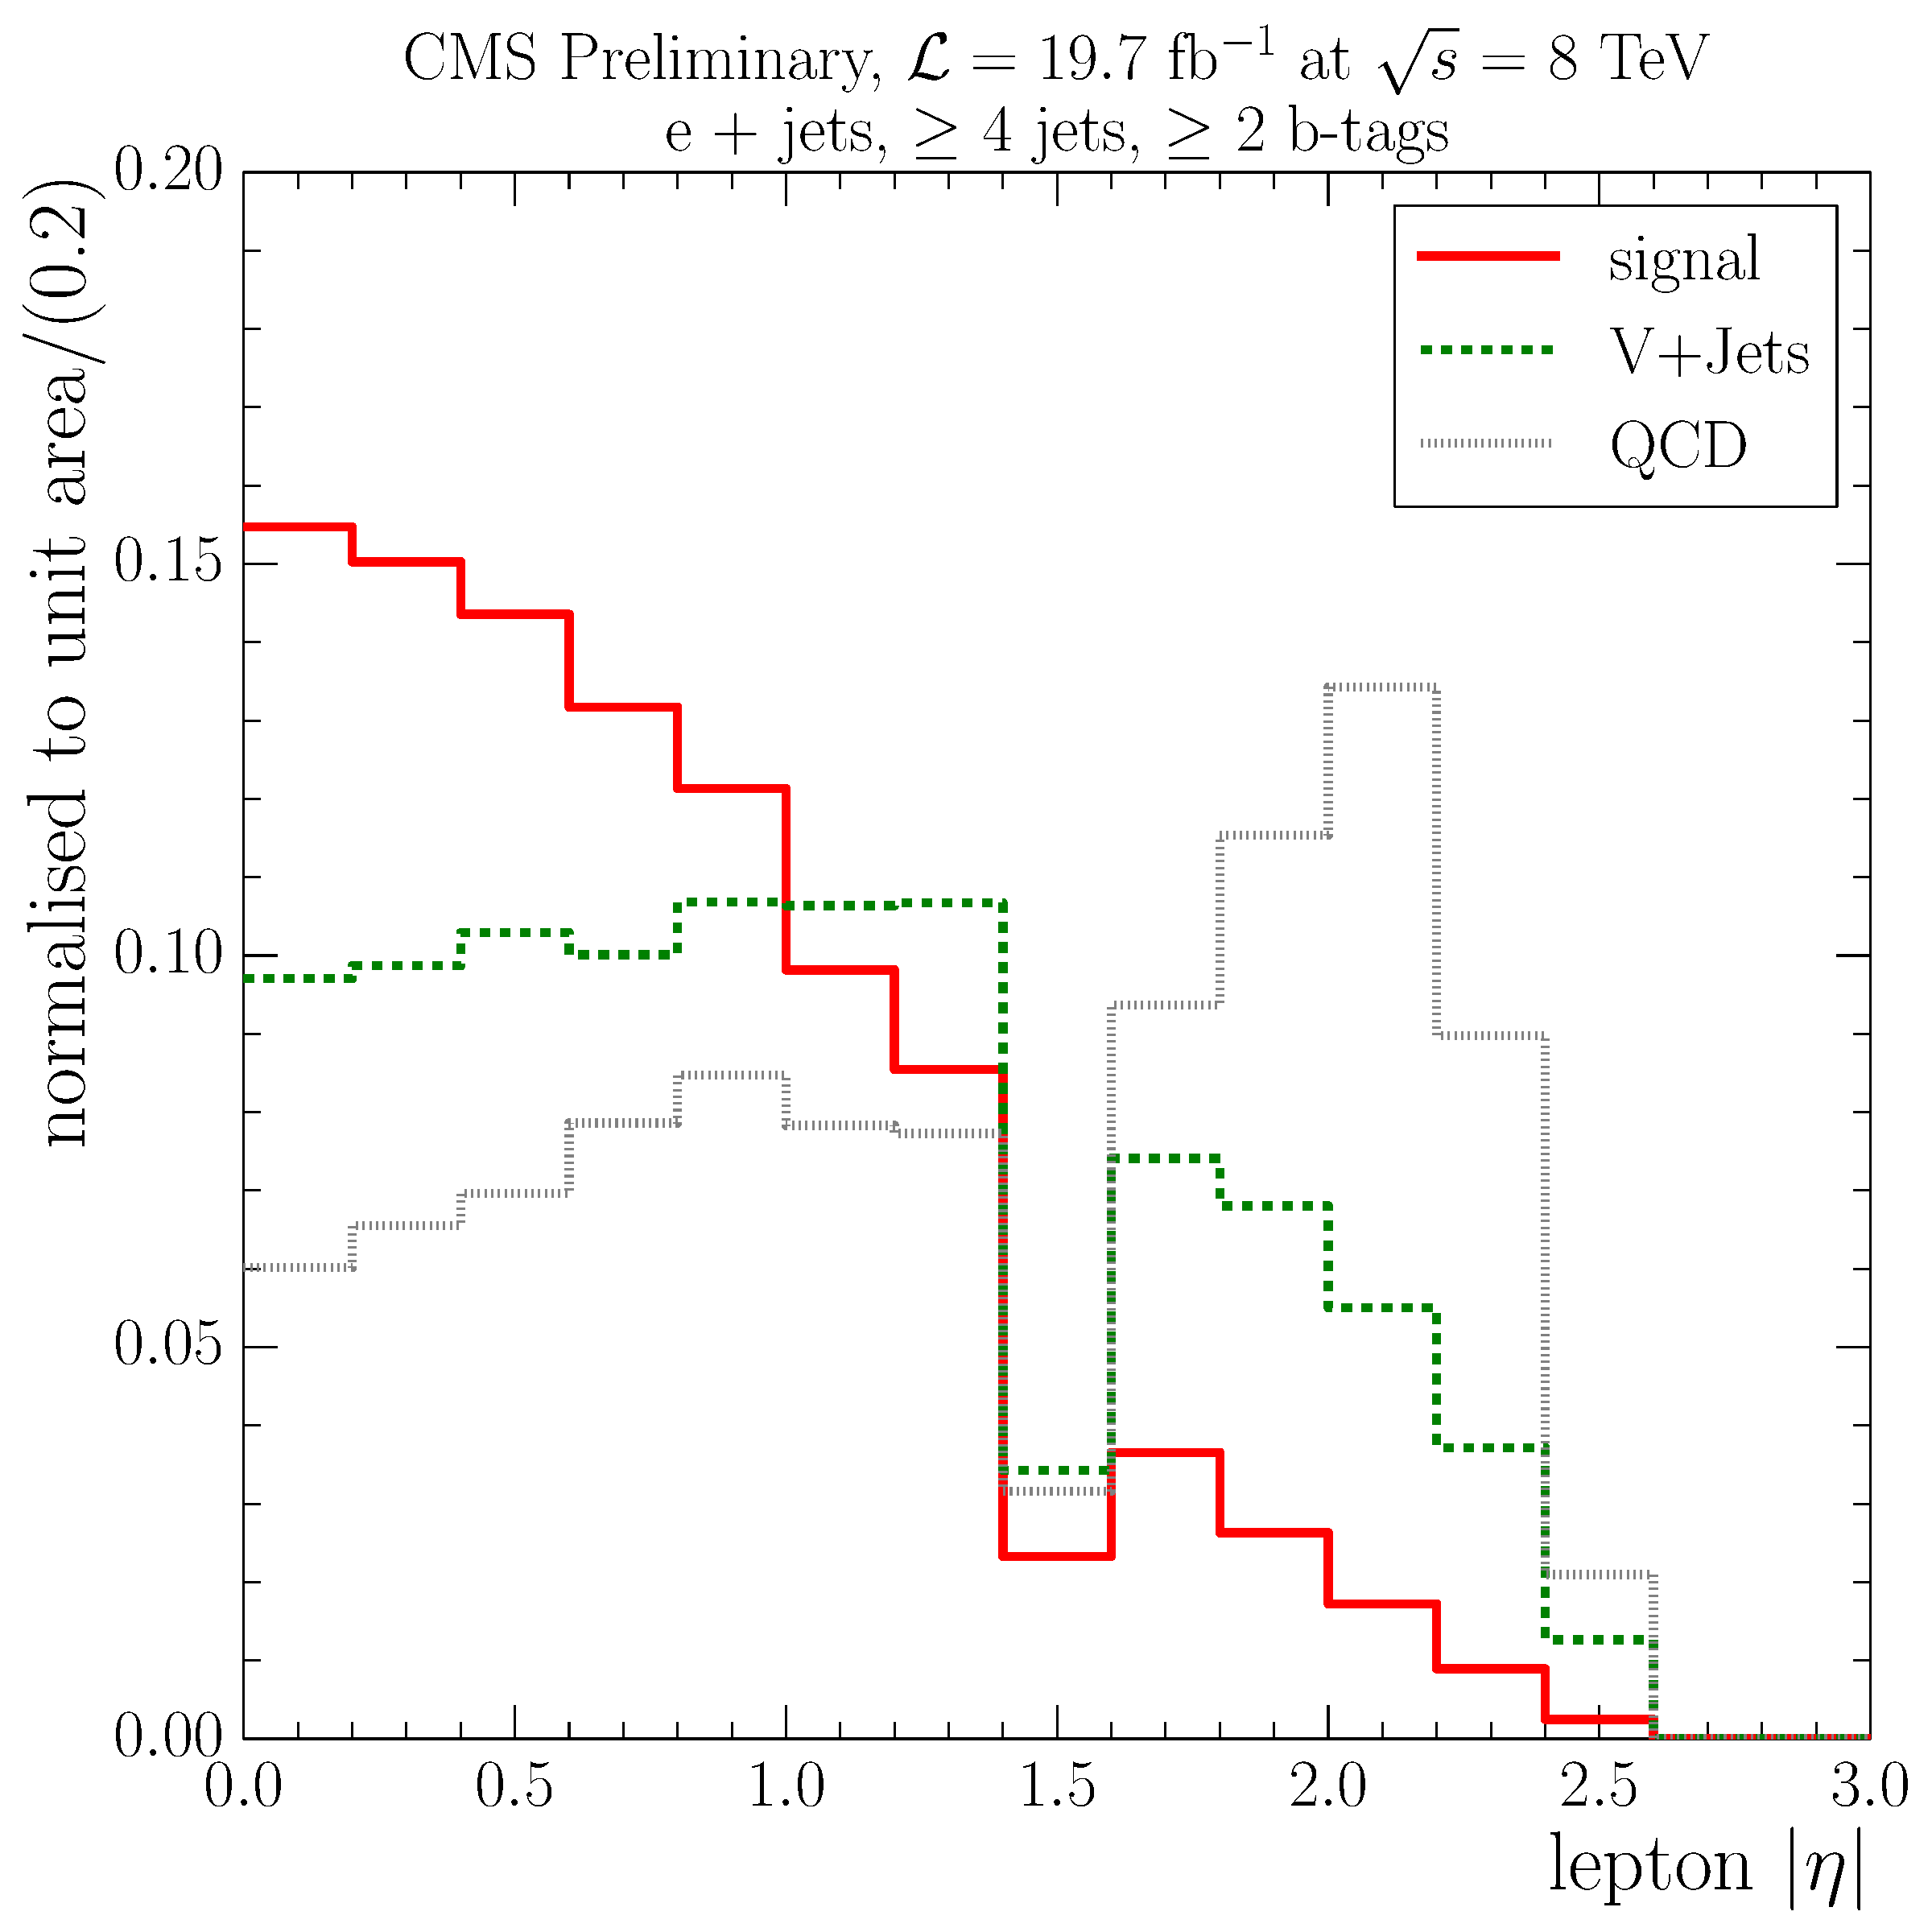
\includegraphics[width=0.3\textwidth]{measurement/MET/central/fit_templates/electron_templates_bin_0-25}}
%   	{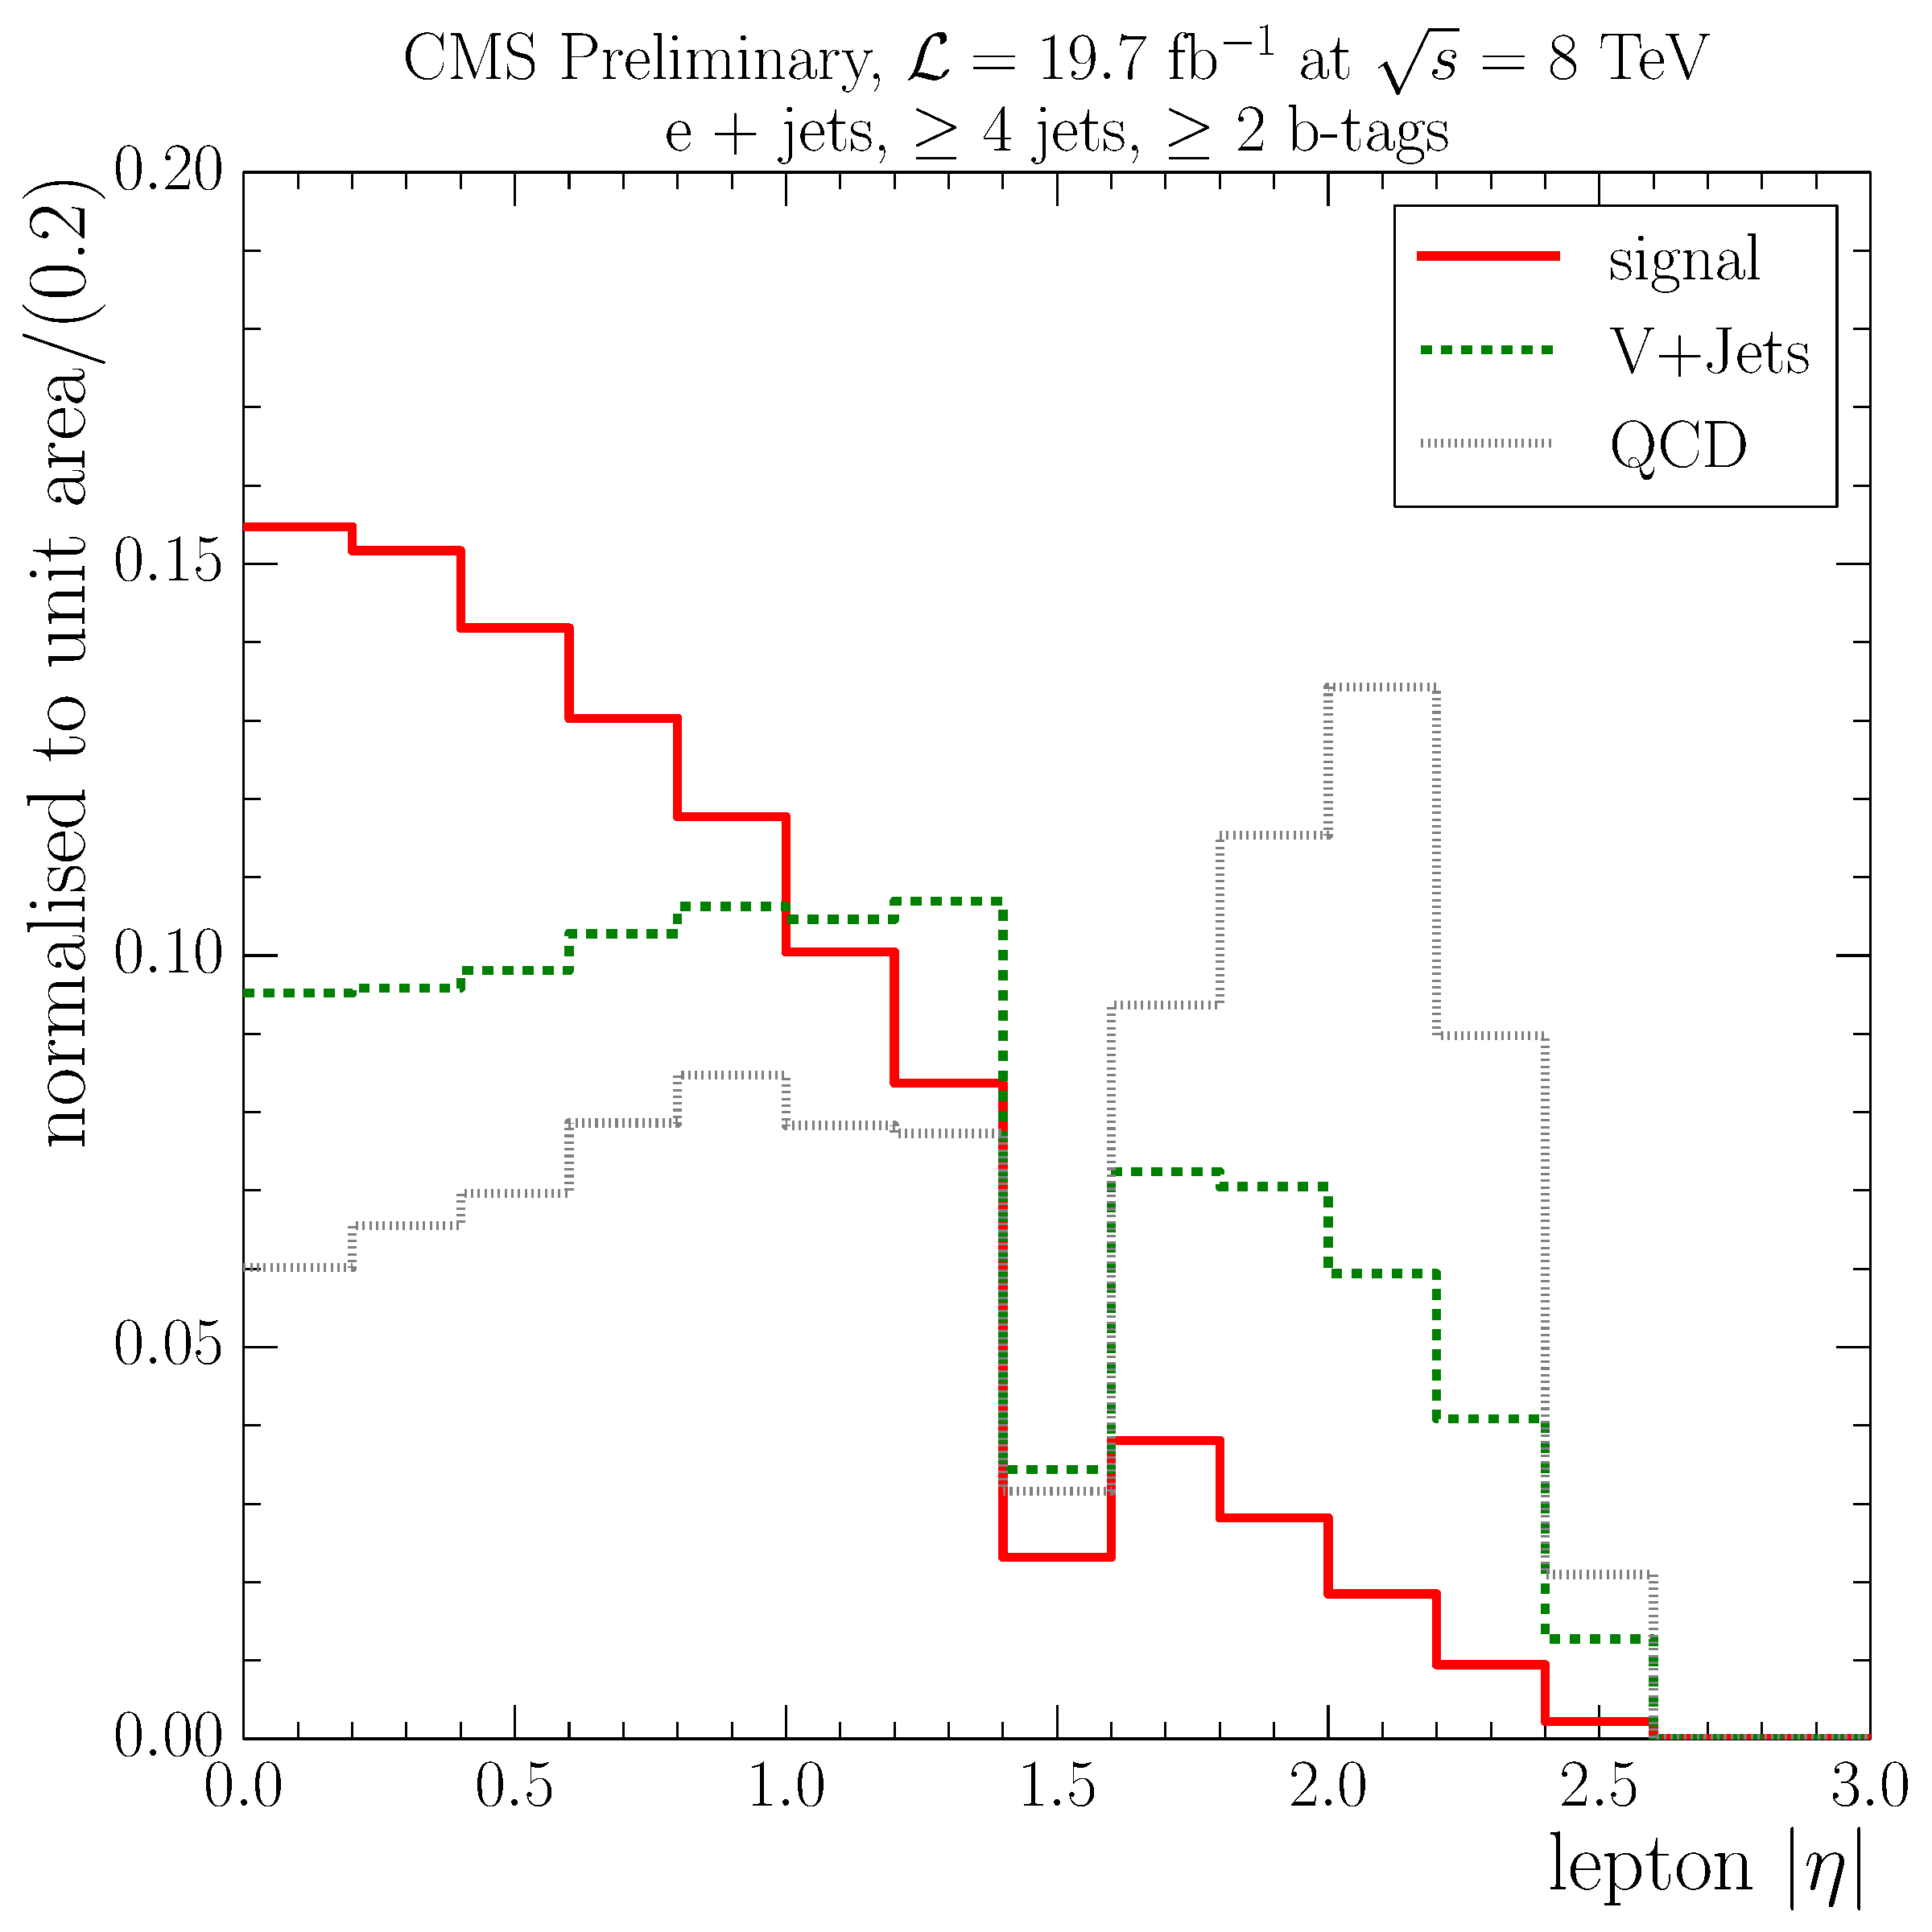
\includegraphics[width=0.3\textwidth]{measurement/MET/central/fit_templates/electron_templates_bin_25-45}}
%   	{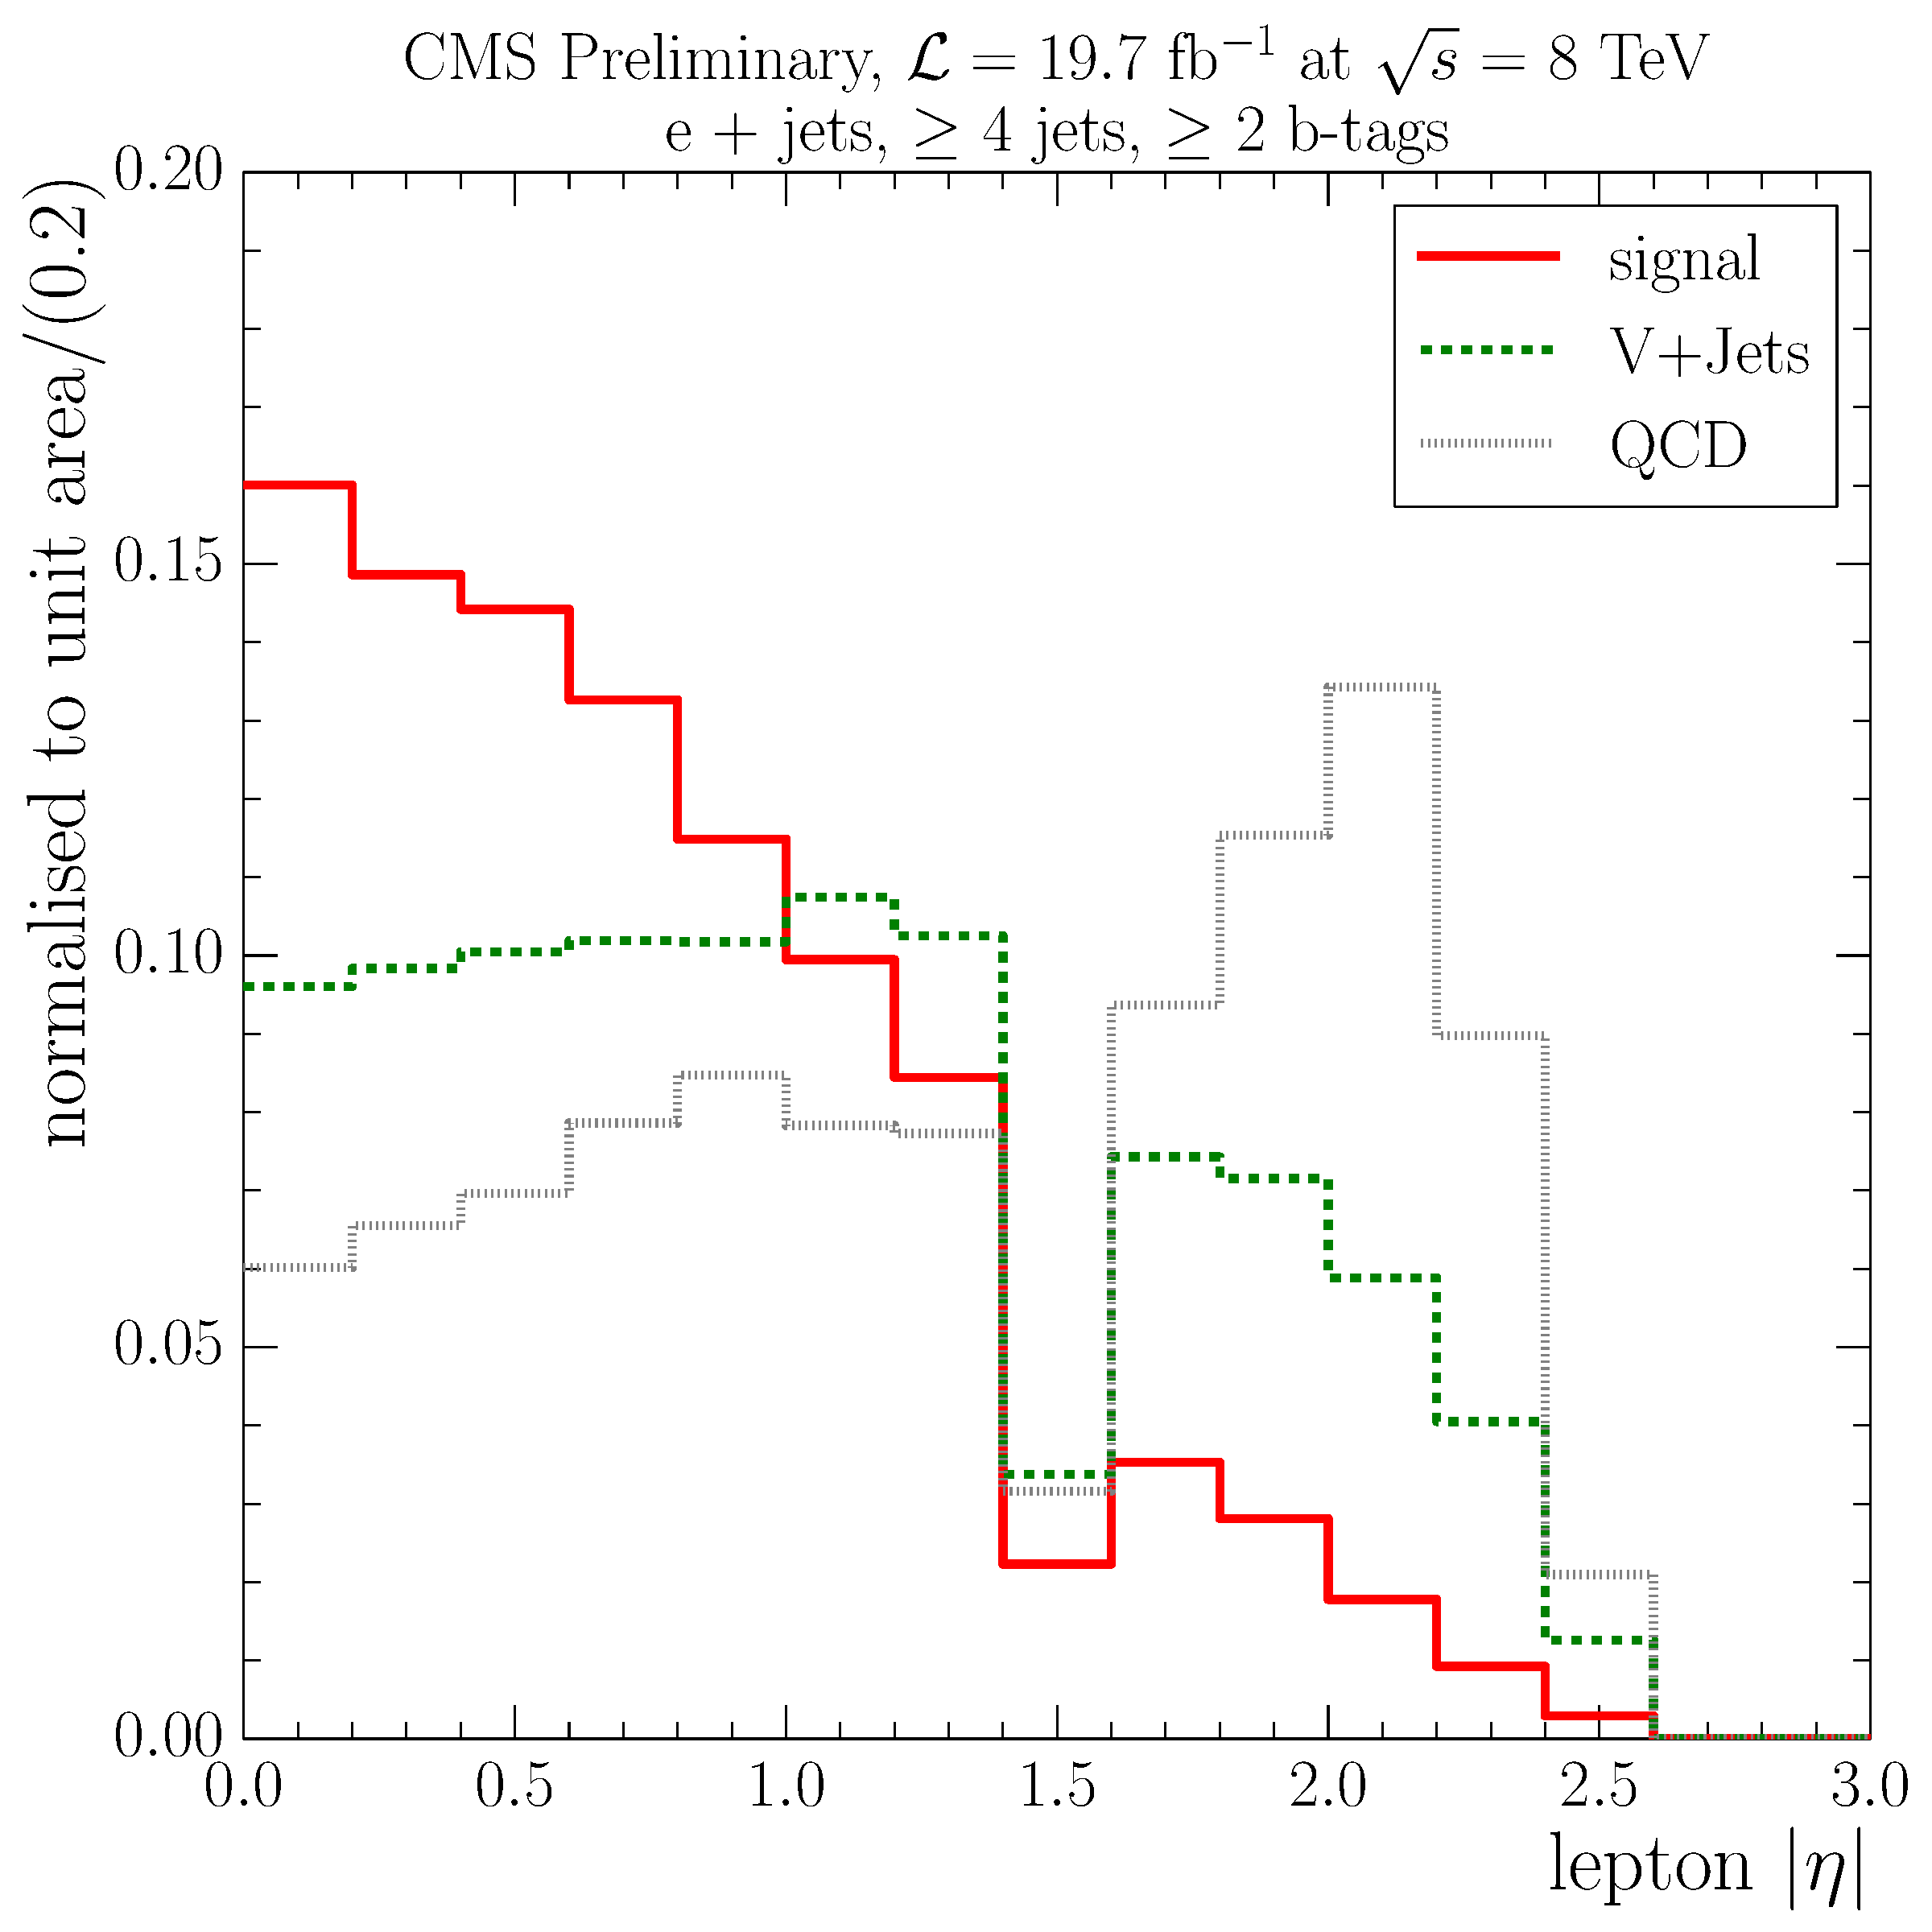
\includegraphics[width=0.3\textwidth]{measurement/MET/central/fit_templates/electron_templates_bin_45-70}}\\
%   	{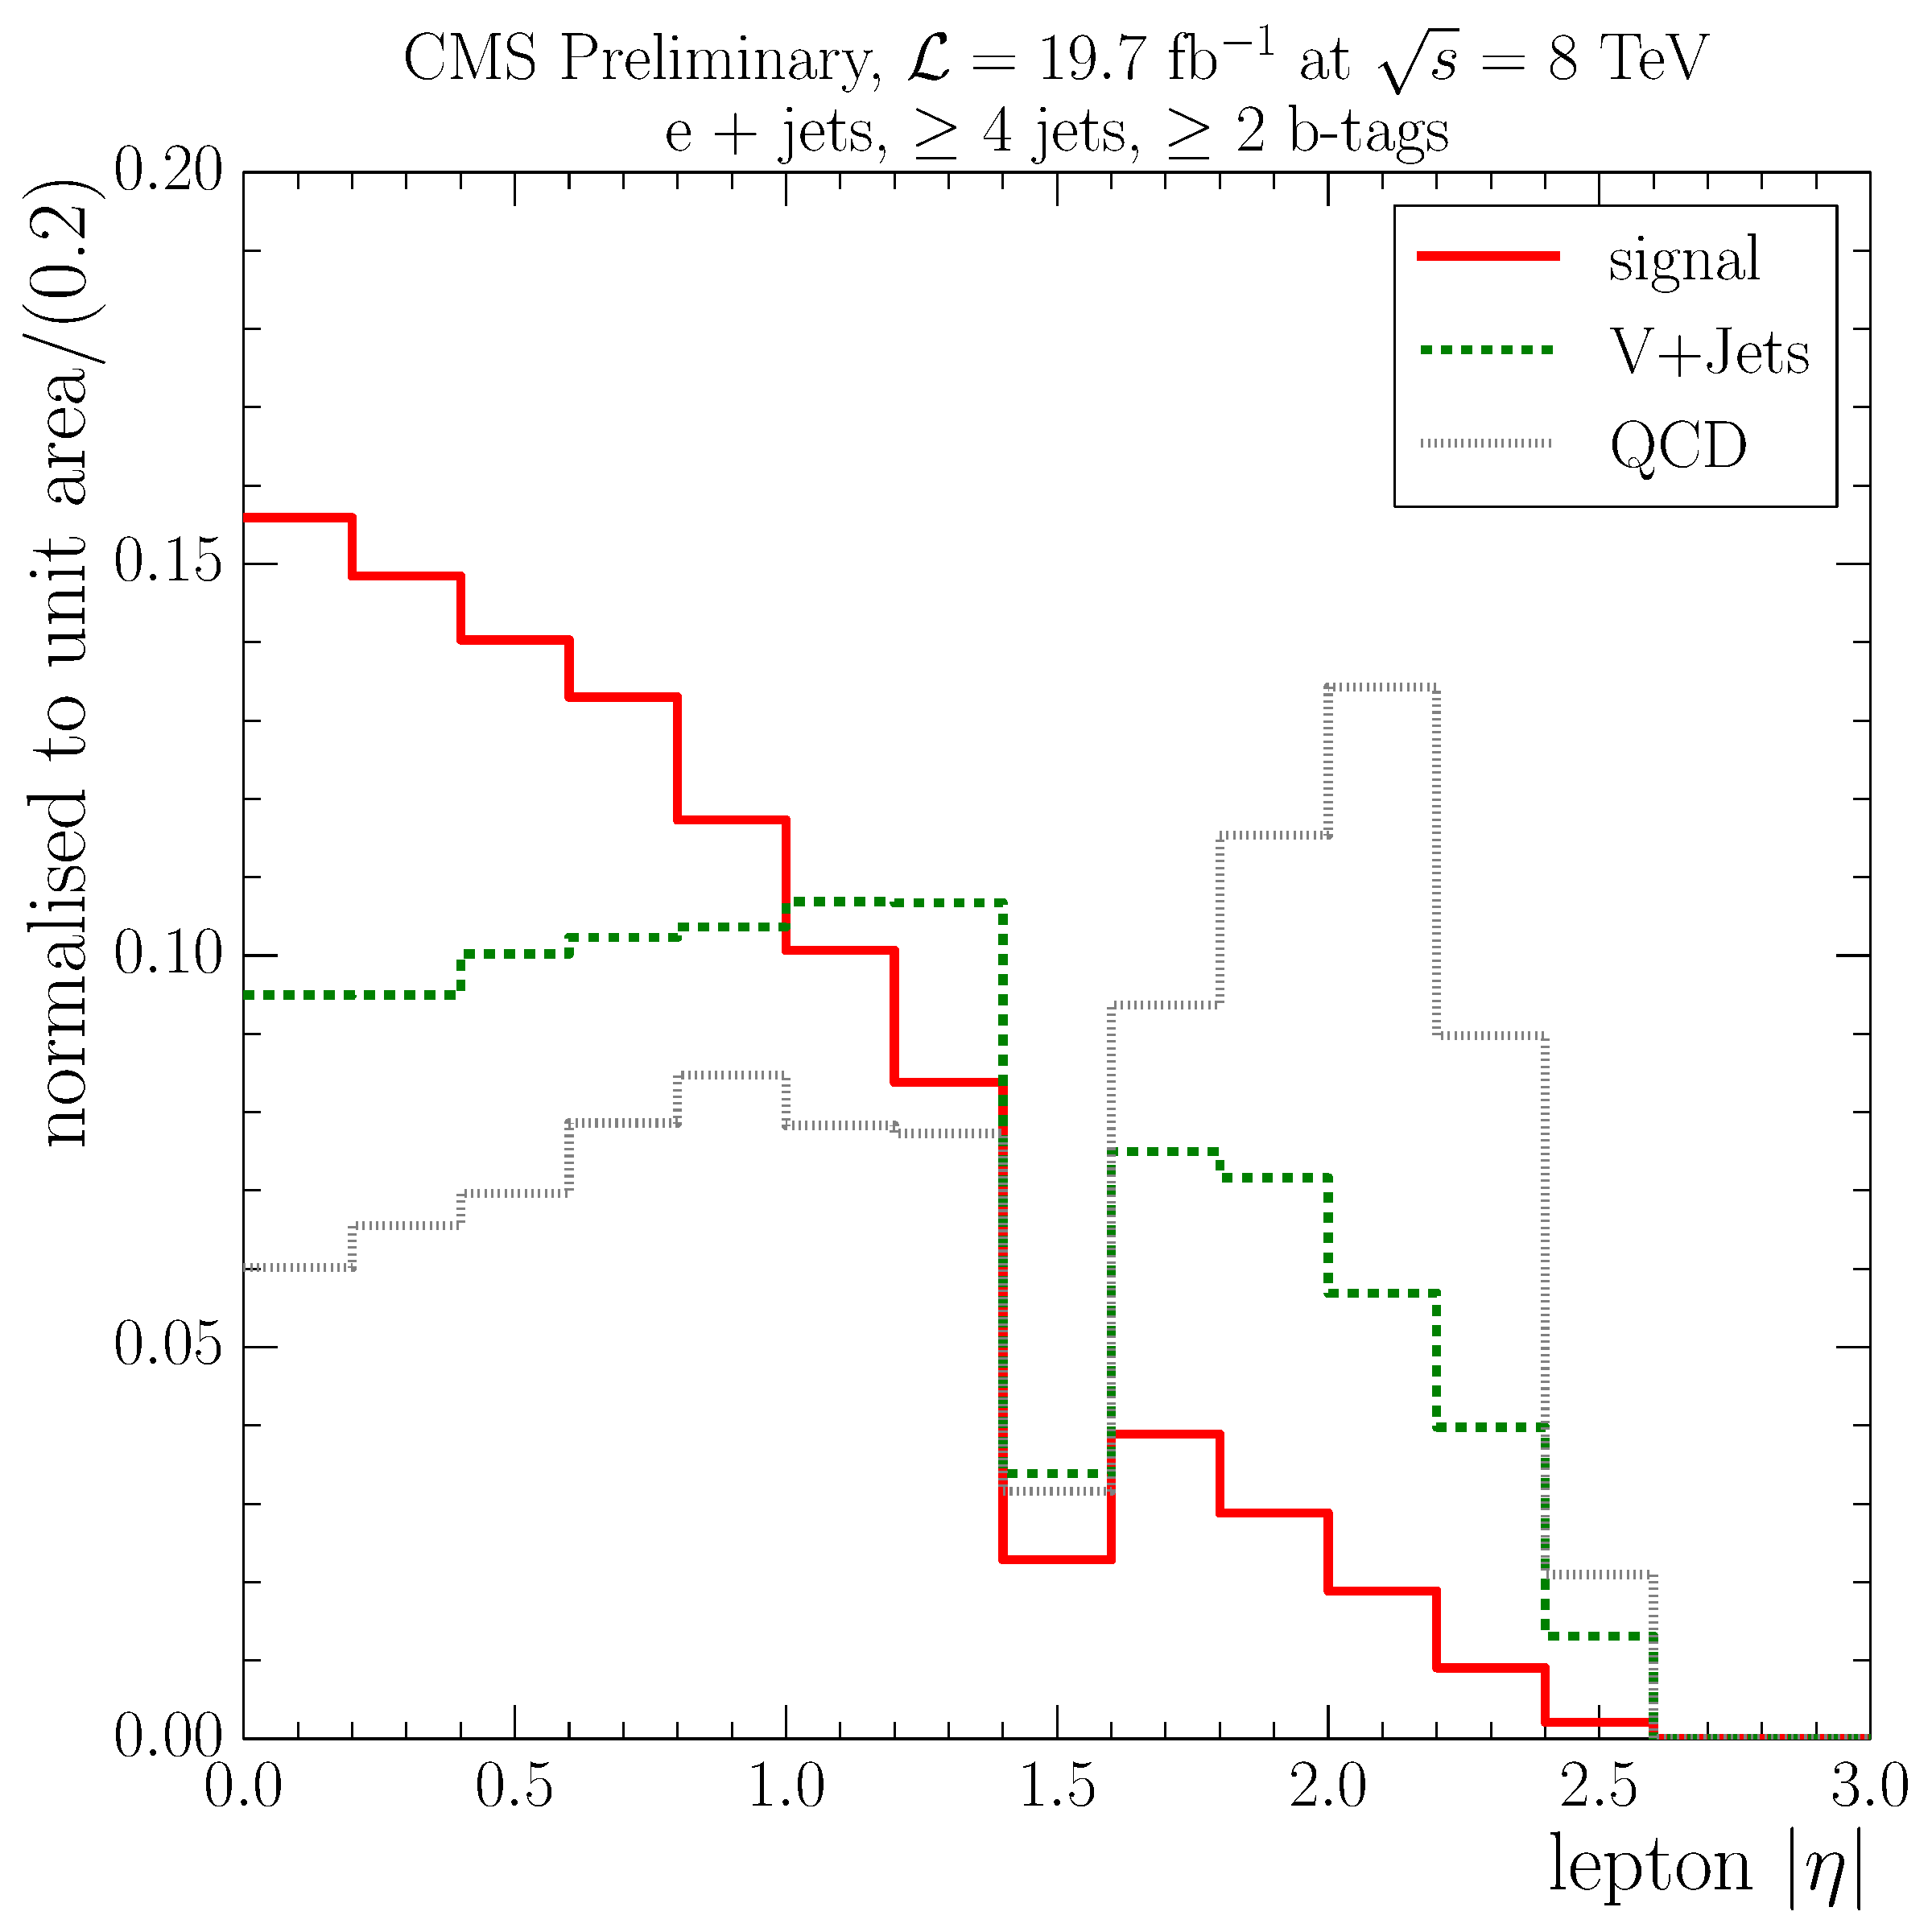
\includegraphics[width=0.3\textwidth]{measurement/MET/central/fit_templates/electron_templates_bin_70-100}}
%   	{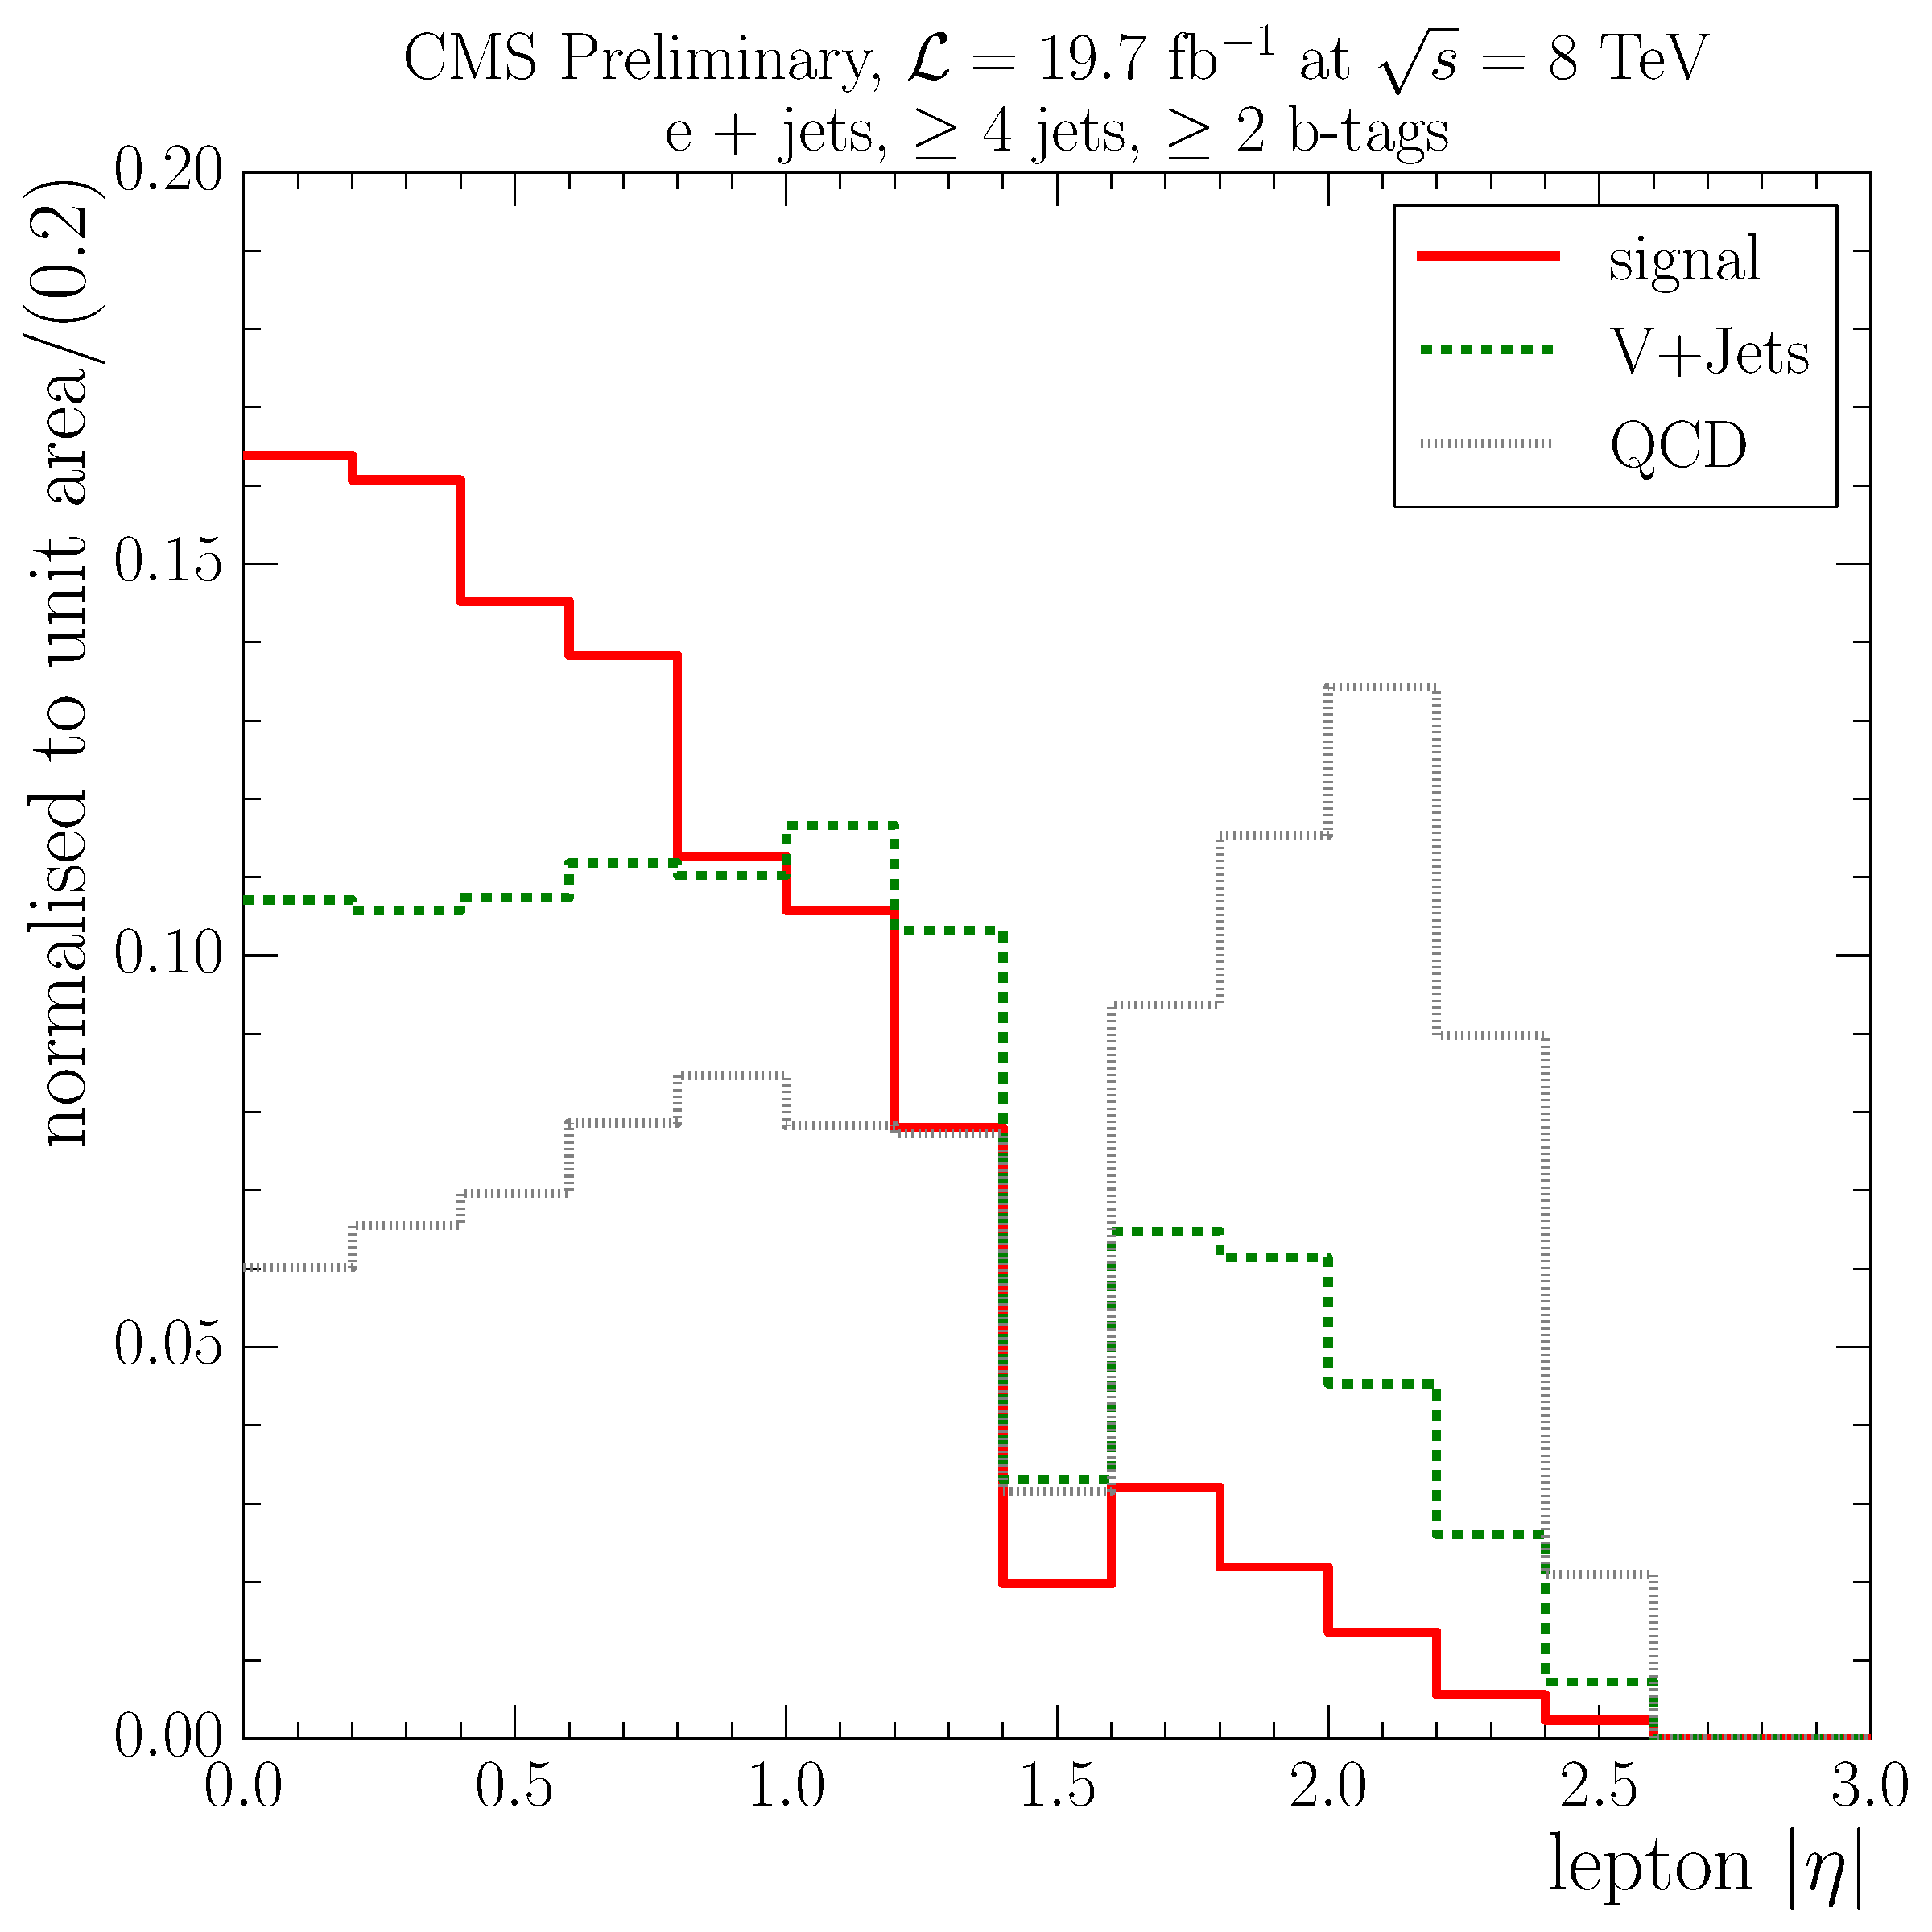
\includegraphics[width=0.3\textwidth]{measurement/MET/central/fit_templates/electron_templates_bin_100-150}}
%   	{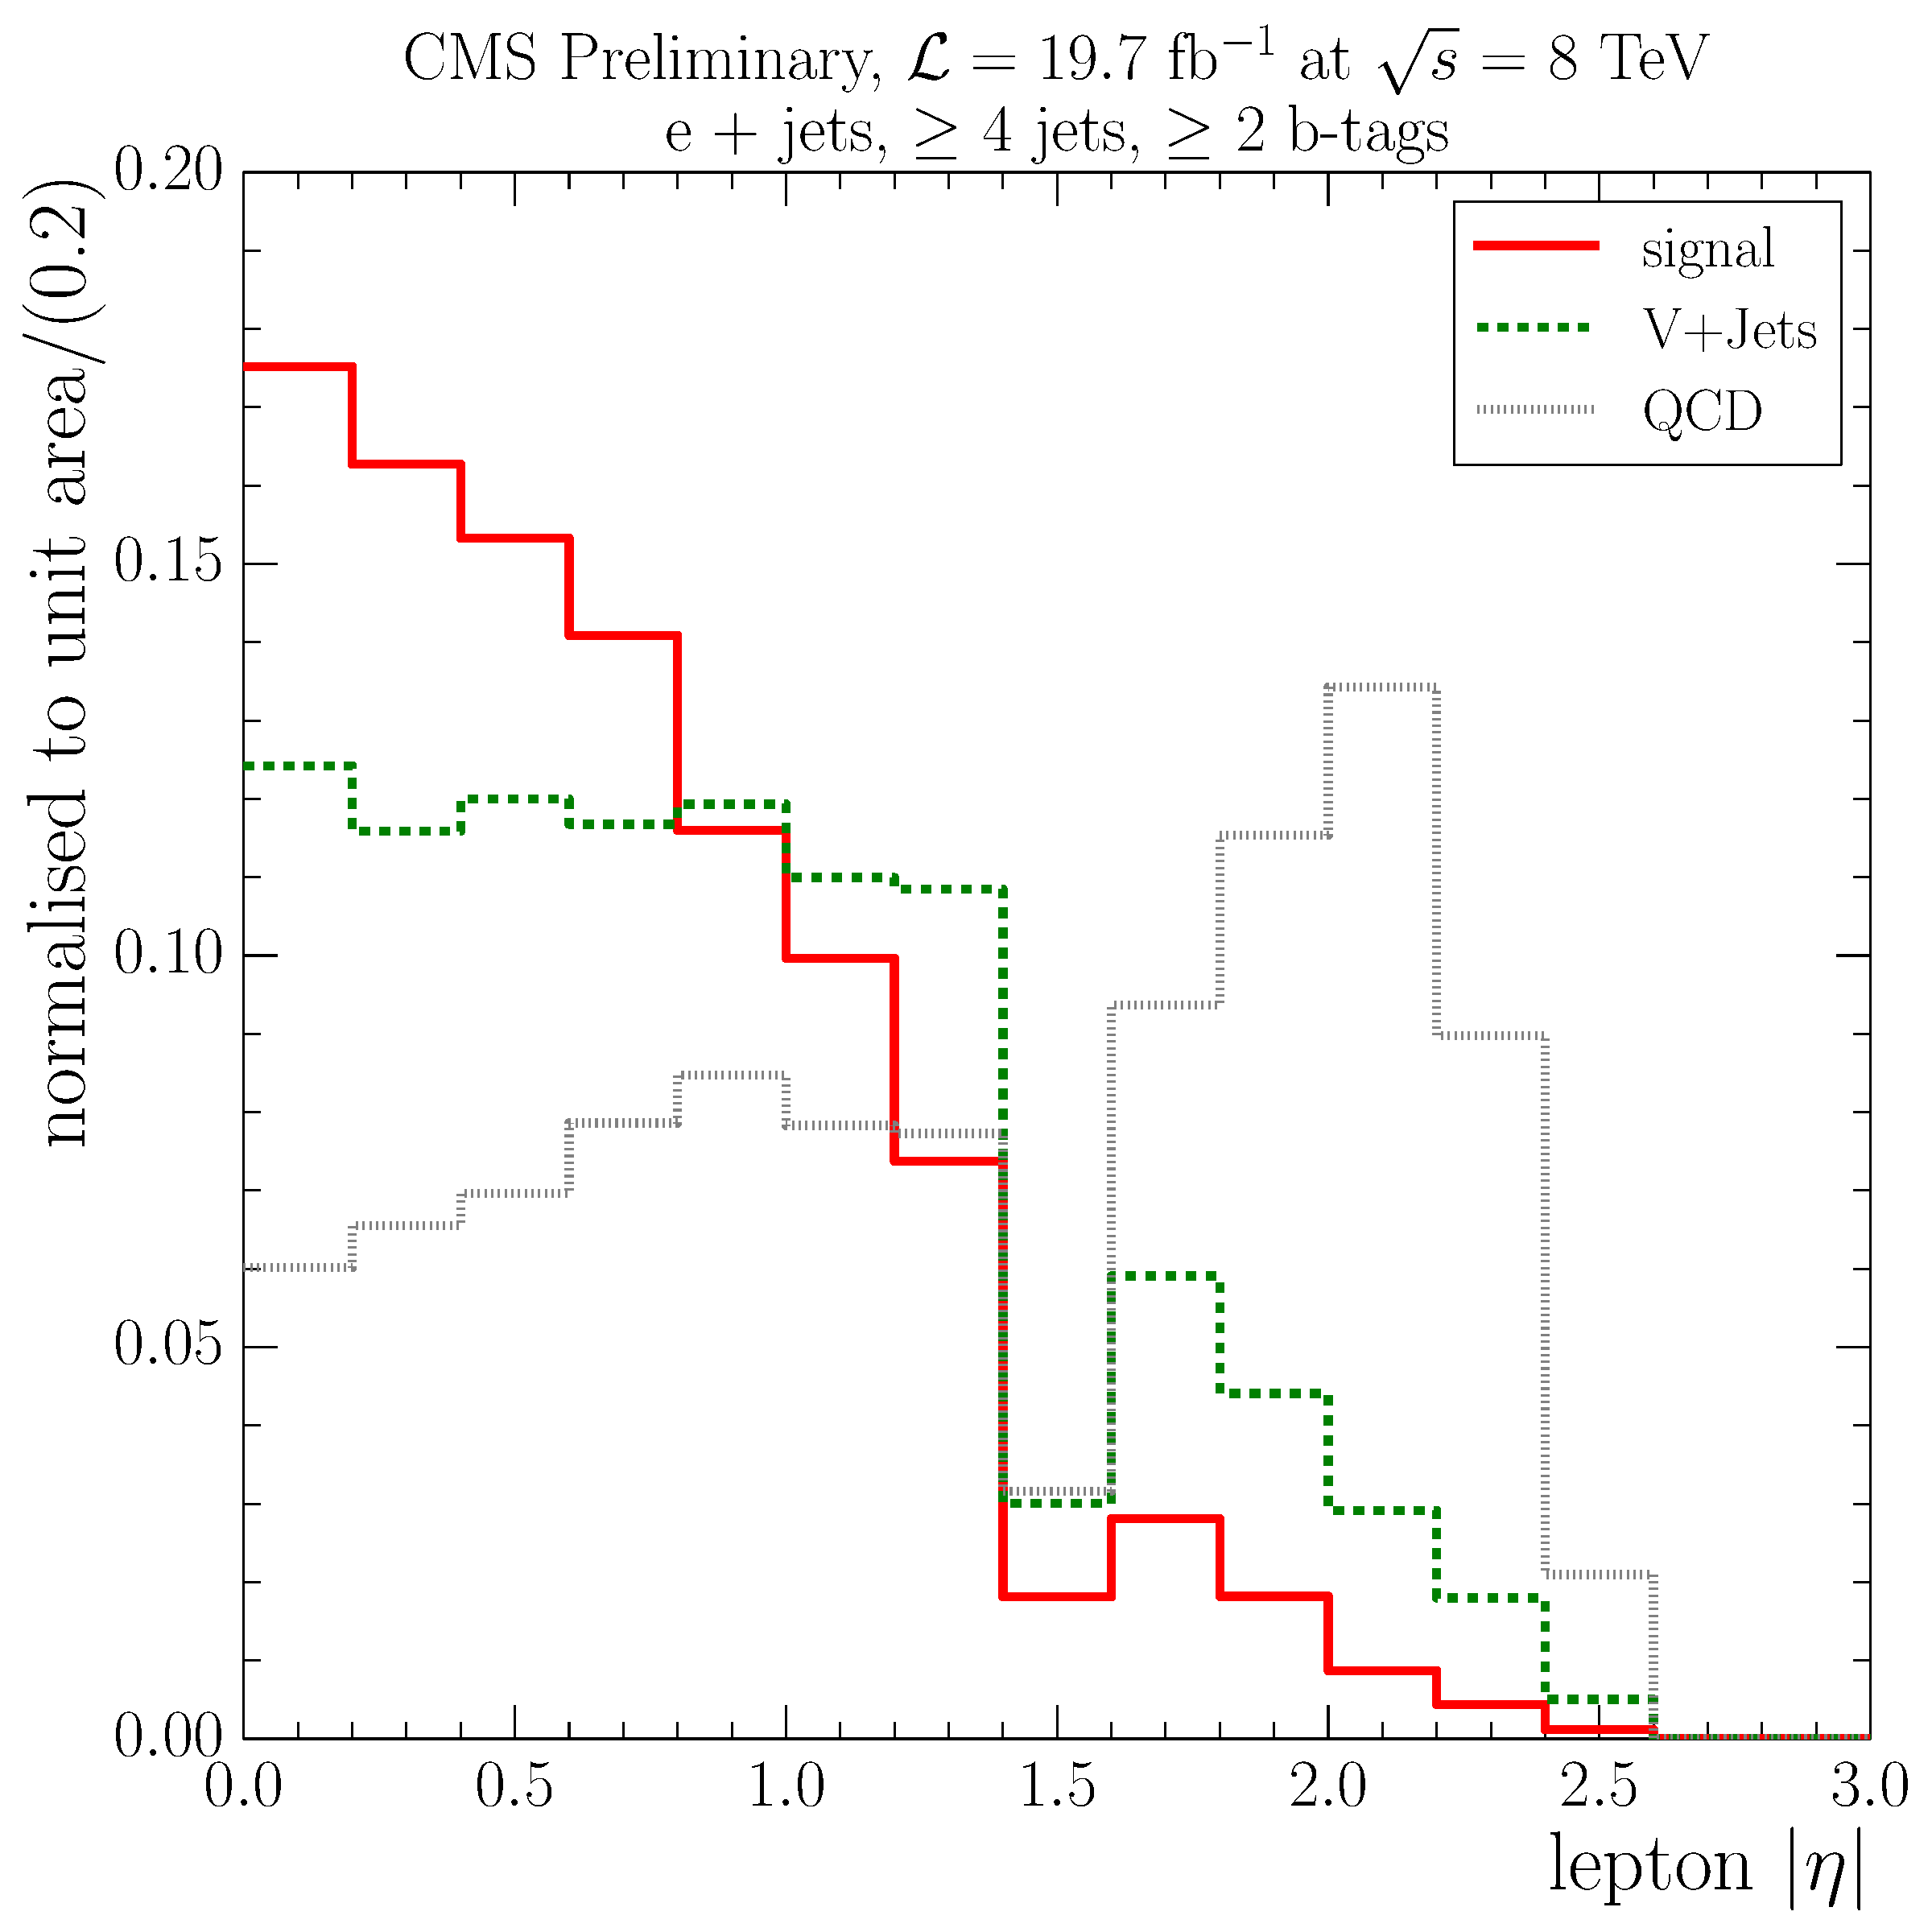
\includegraphics[width=0.3\textwidth]{measurement/MET/central/fit_templates/electron_templates_bin_150-inf}}
%     \caption{Distributions of electron $\abs \eta$ with the results of the template fit in
%     different bins of \MET, from top left to bottom right: \SIrange{0}{25}{\GeV}, \SIrange{25}{45}{\GeV},
%     \SIrange{45}{70}{\GeV}, \SIrange{70}{100}{\GeV}, \SIrange{100}{150}{\GeV} and $\geq \SI{150}{\GeV}$.}
%     \label{fig:fit_results_MET_electron}
% \end{figure}

% \begin{figure}[!htbp]
% 	\centering
%   	{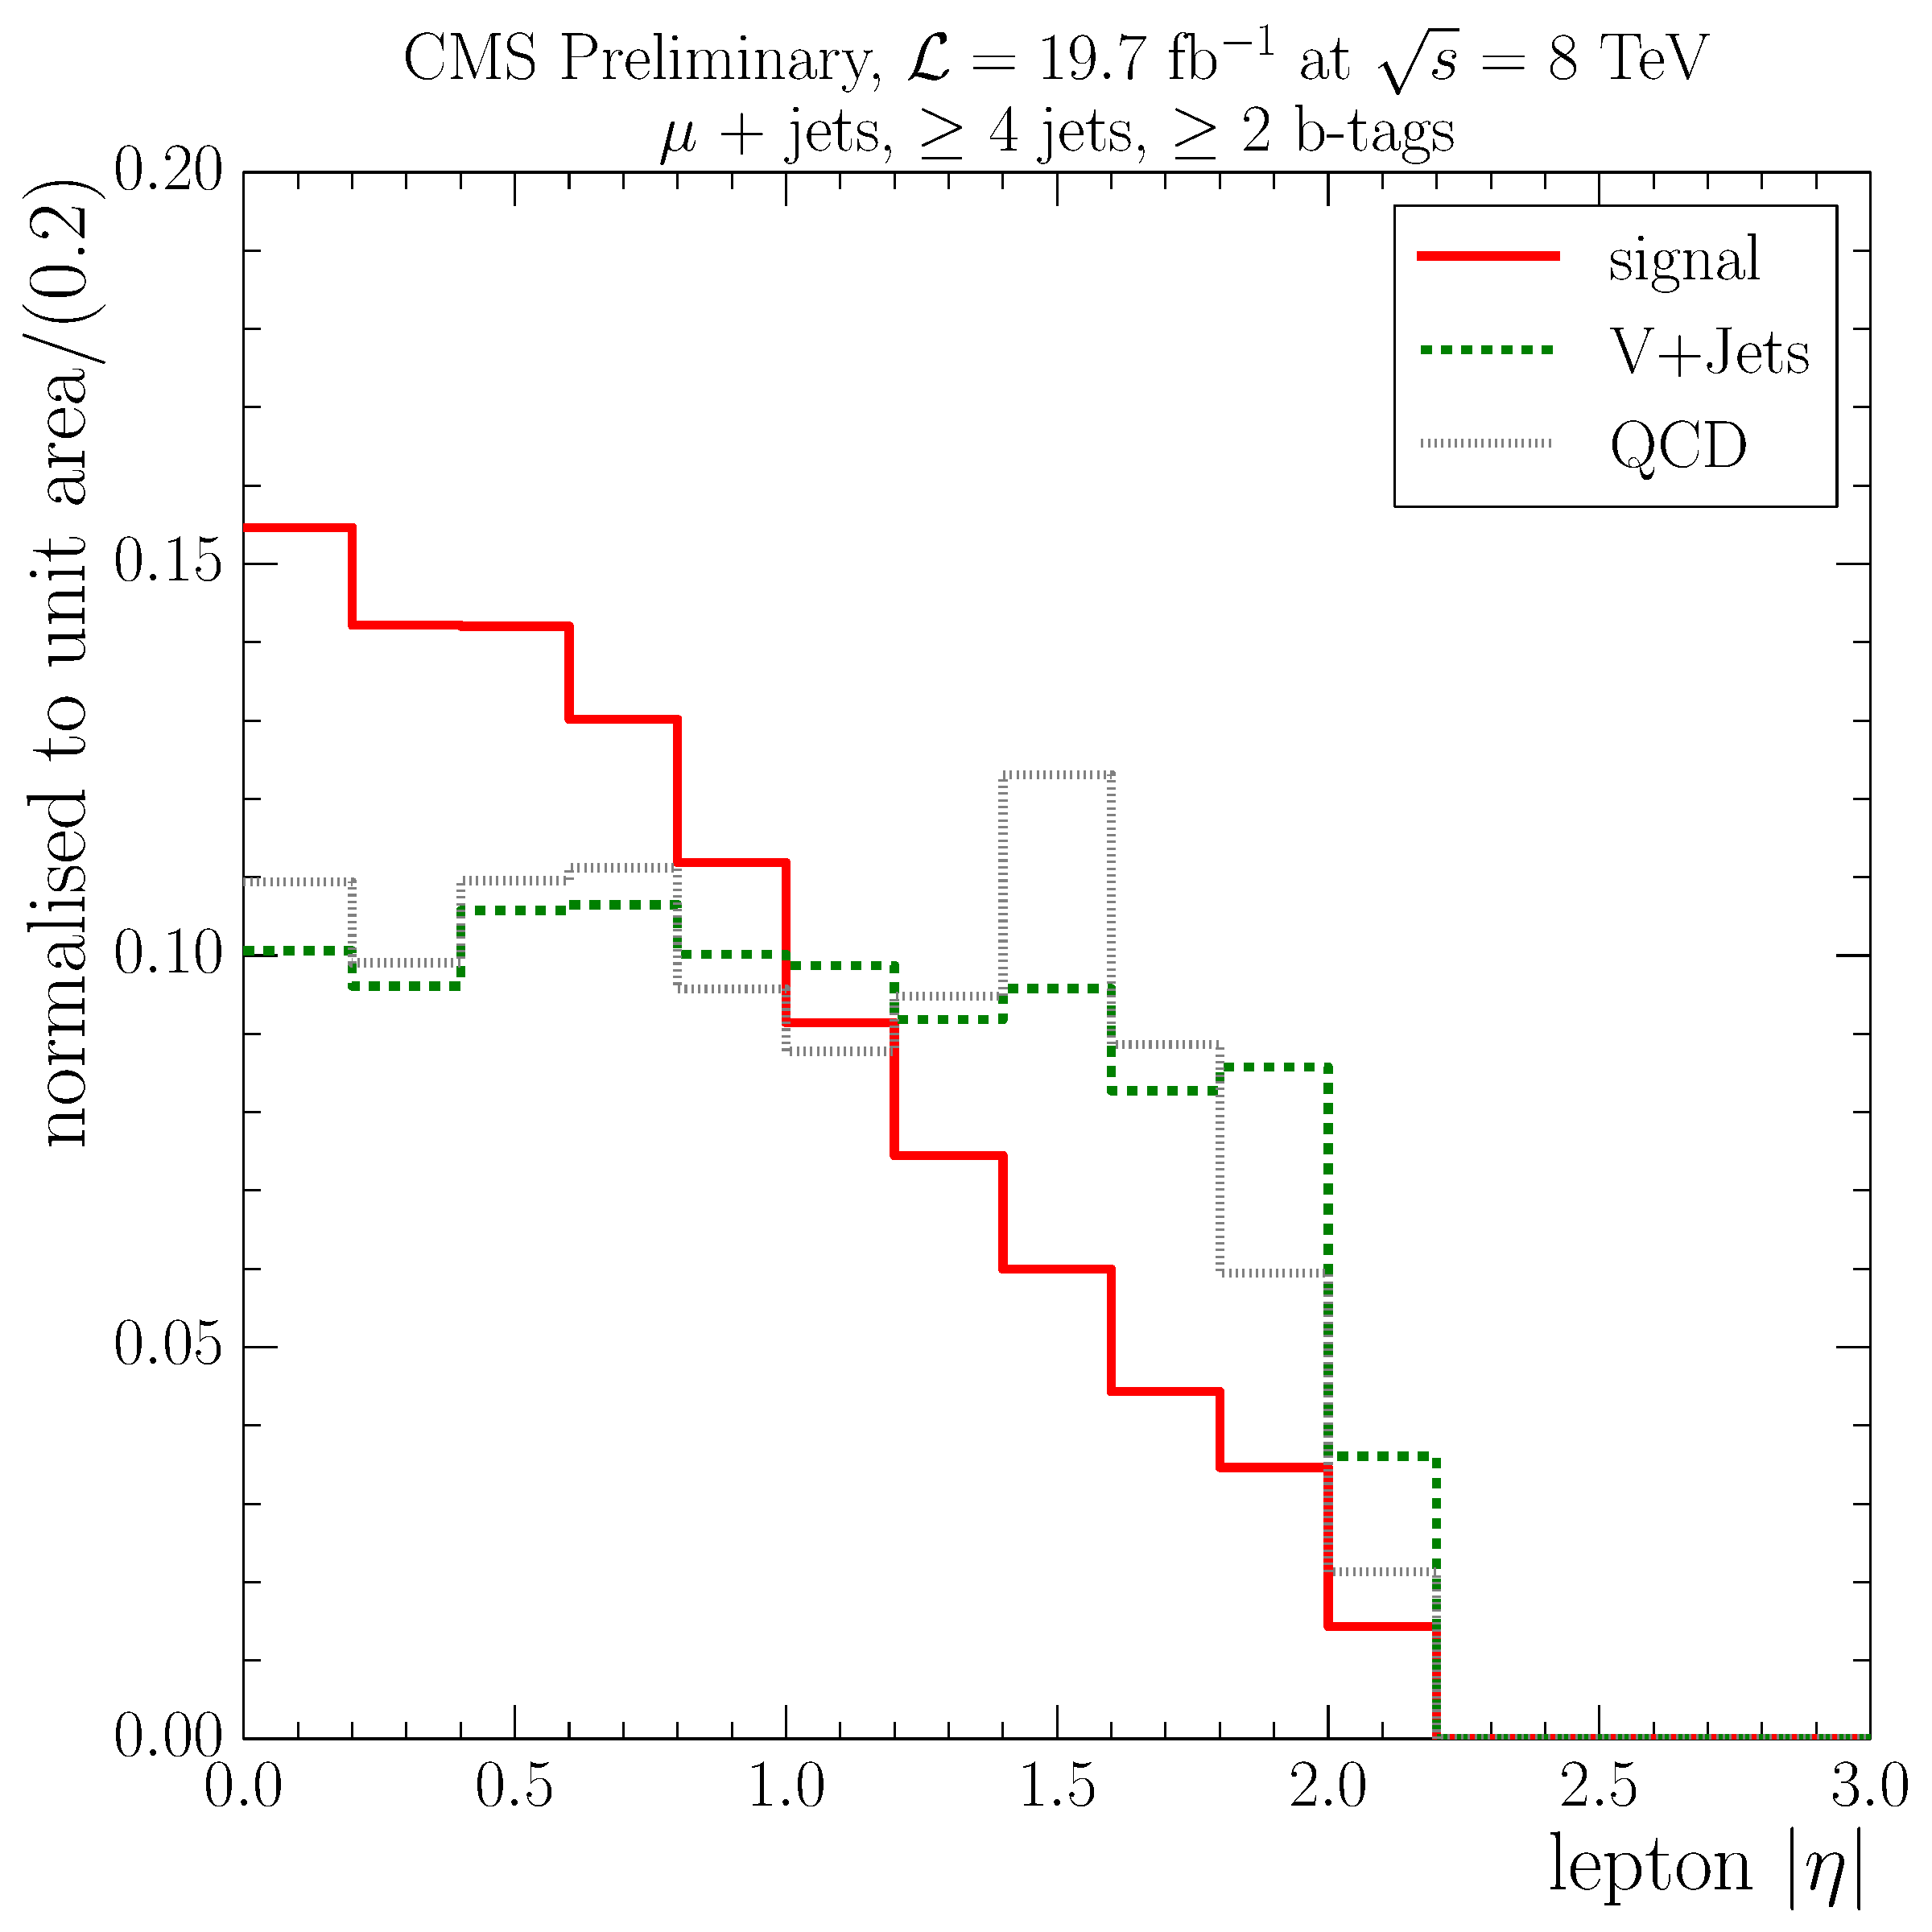
\includegraphics[width=0.3\textwidth]{measurement/MET/central/fit_templates/muon_templates_bin_0-25}}
%   	{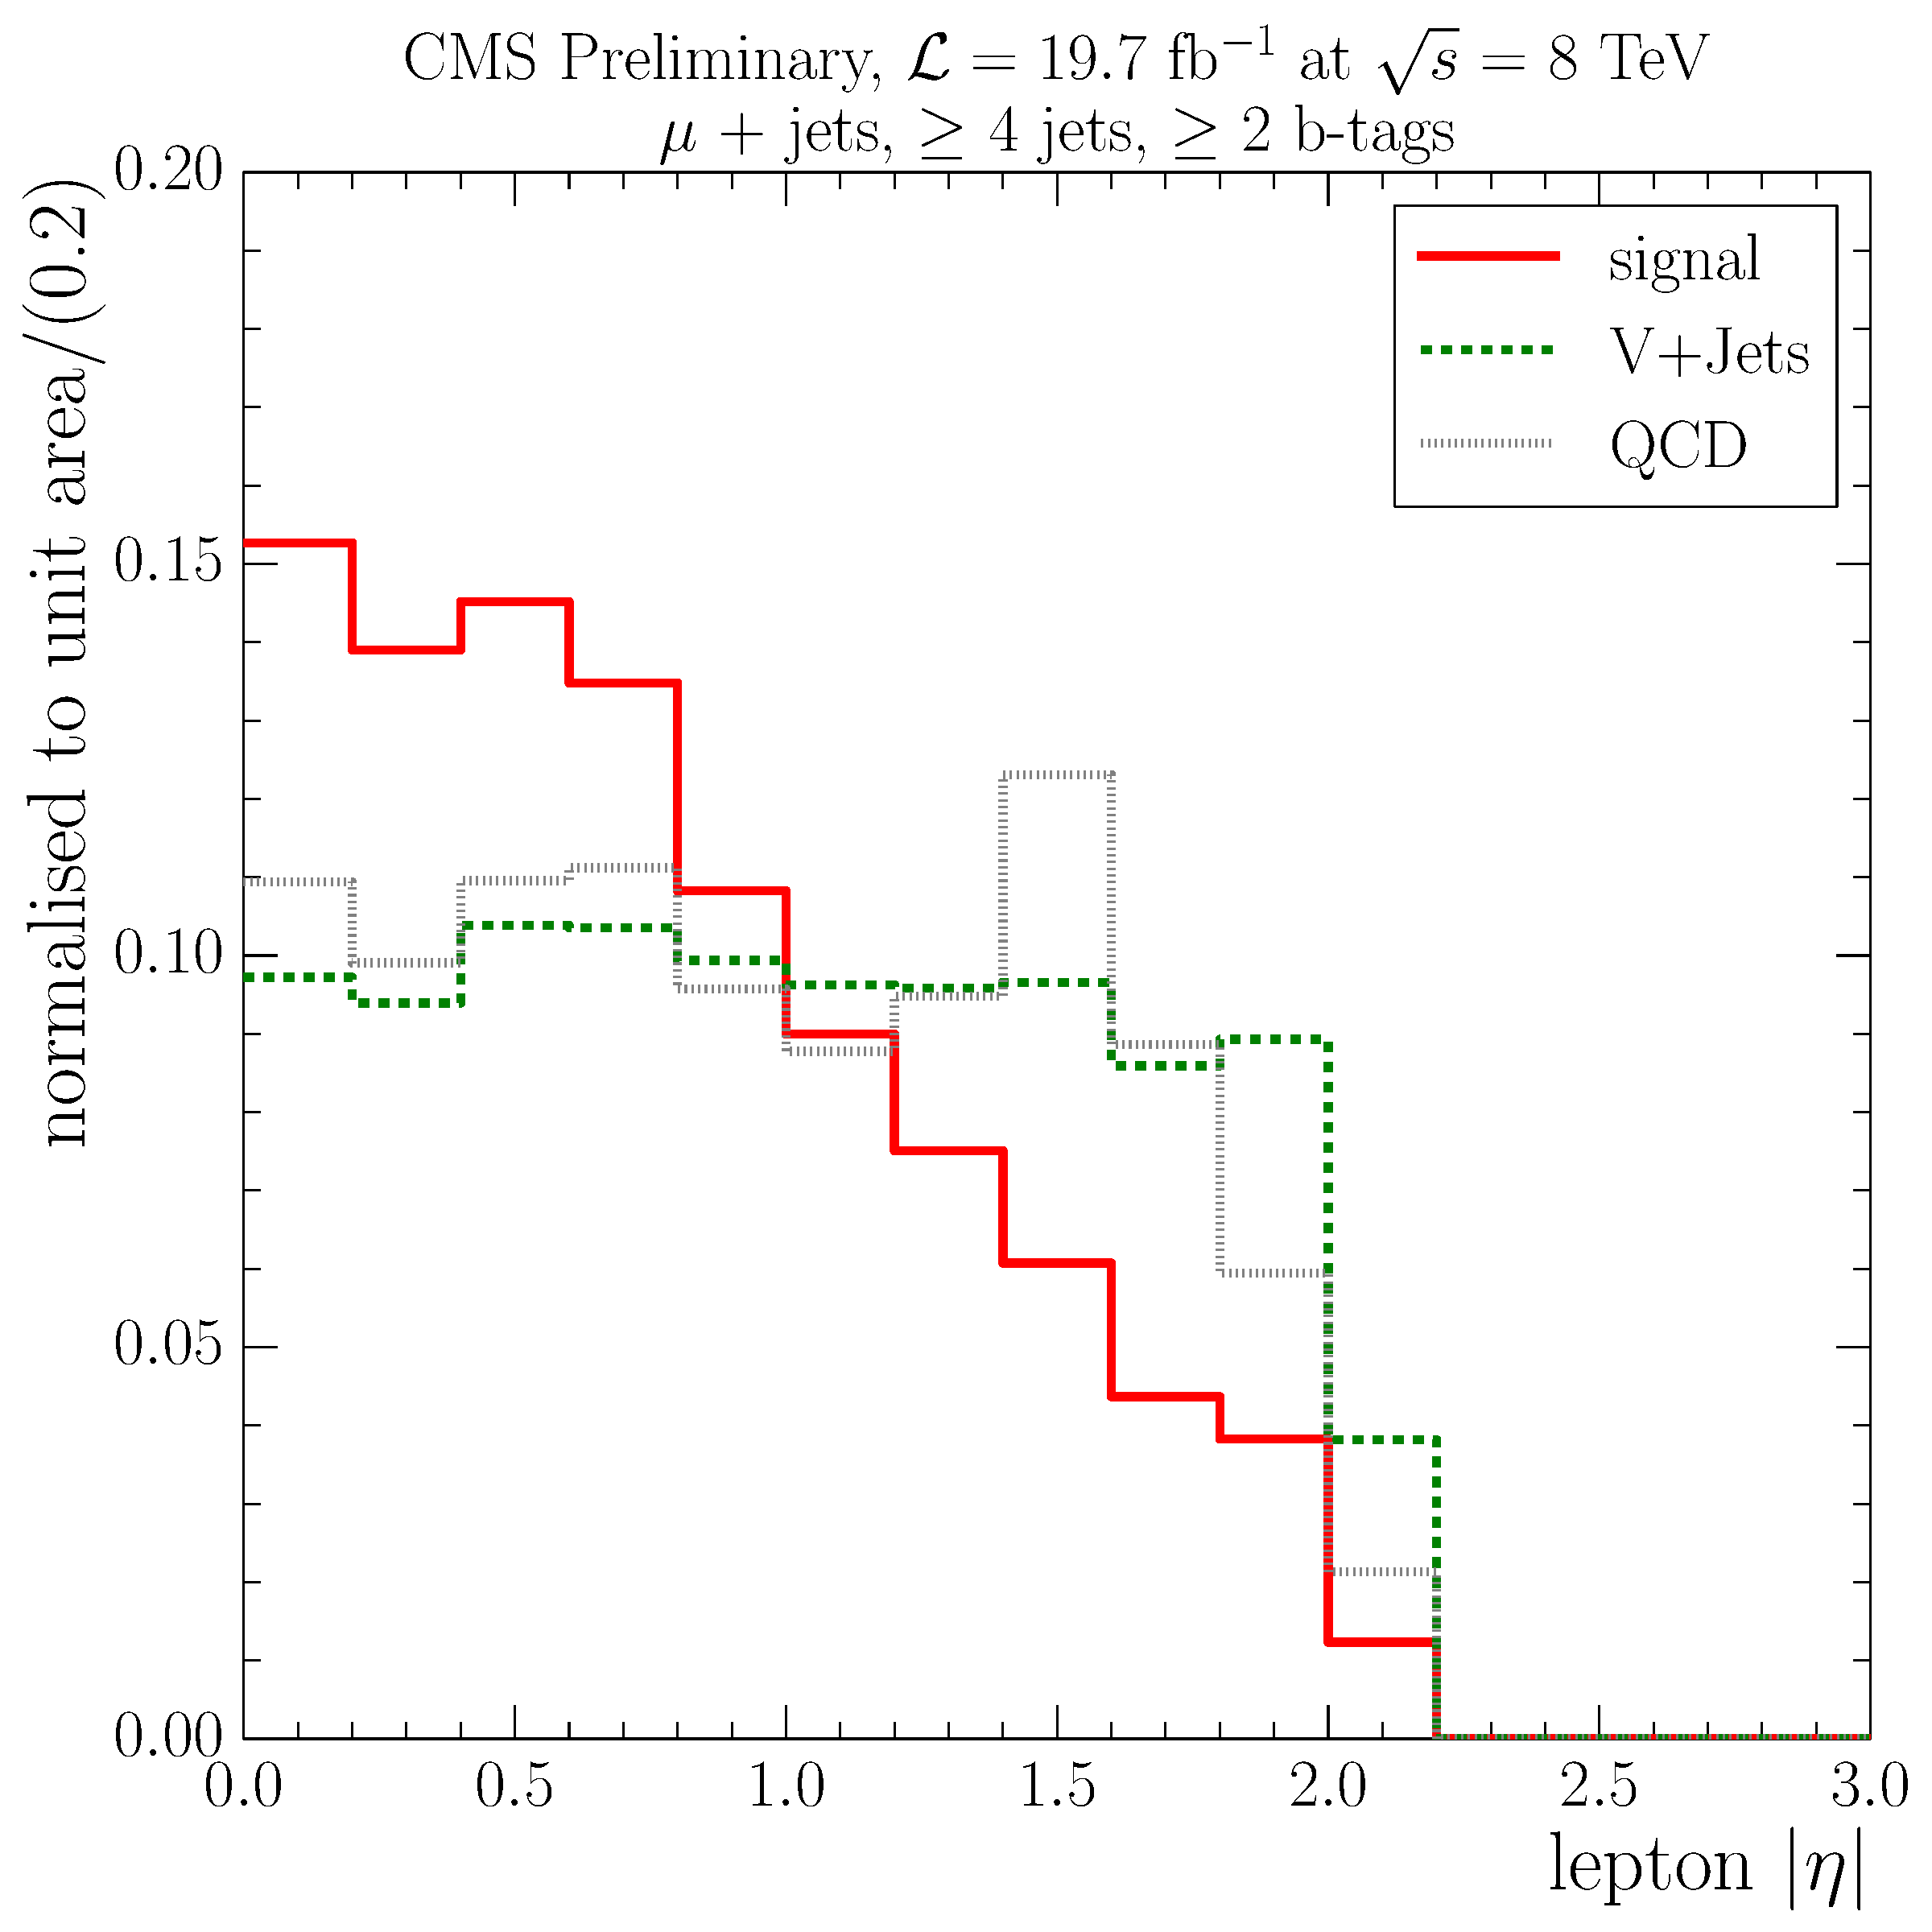
\includegraphics[width=0.3\textwidth]{measurement/MET/central/fit_templates/muon_templates_bin_25-45}}
%   	{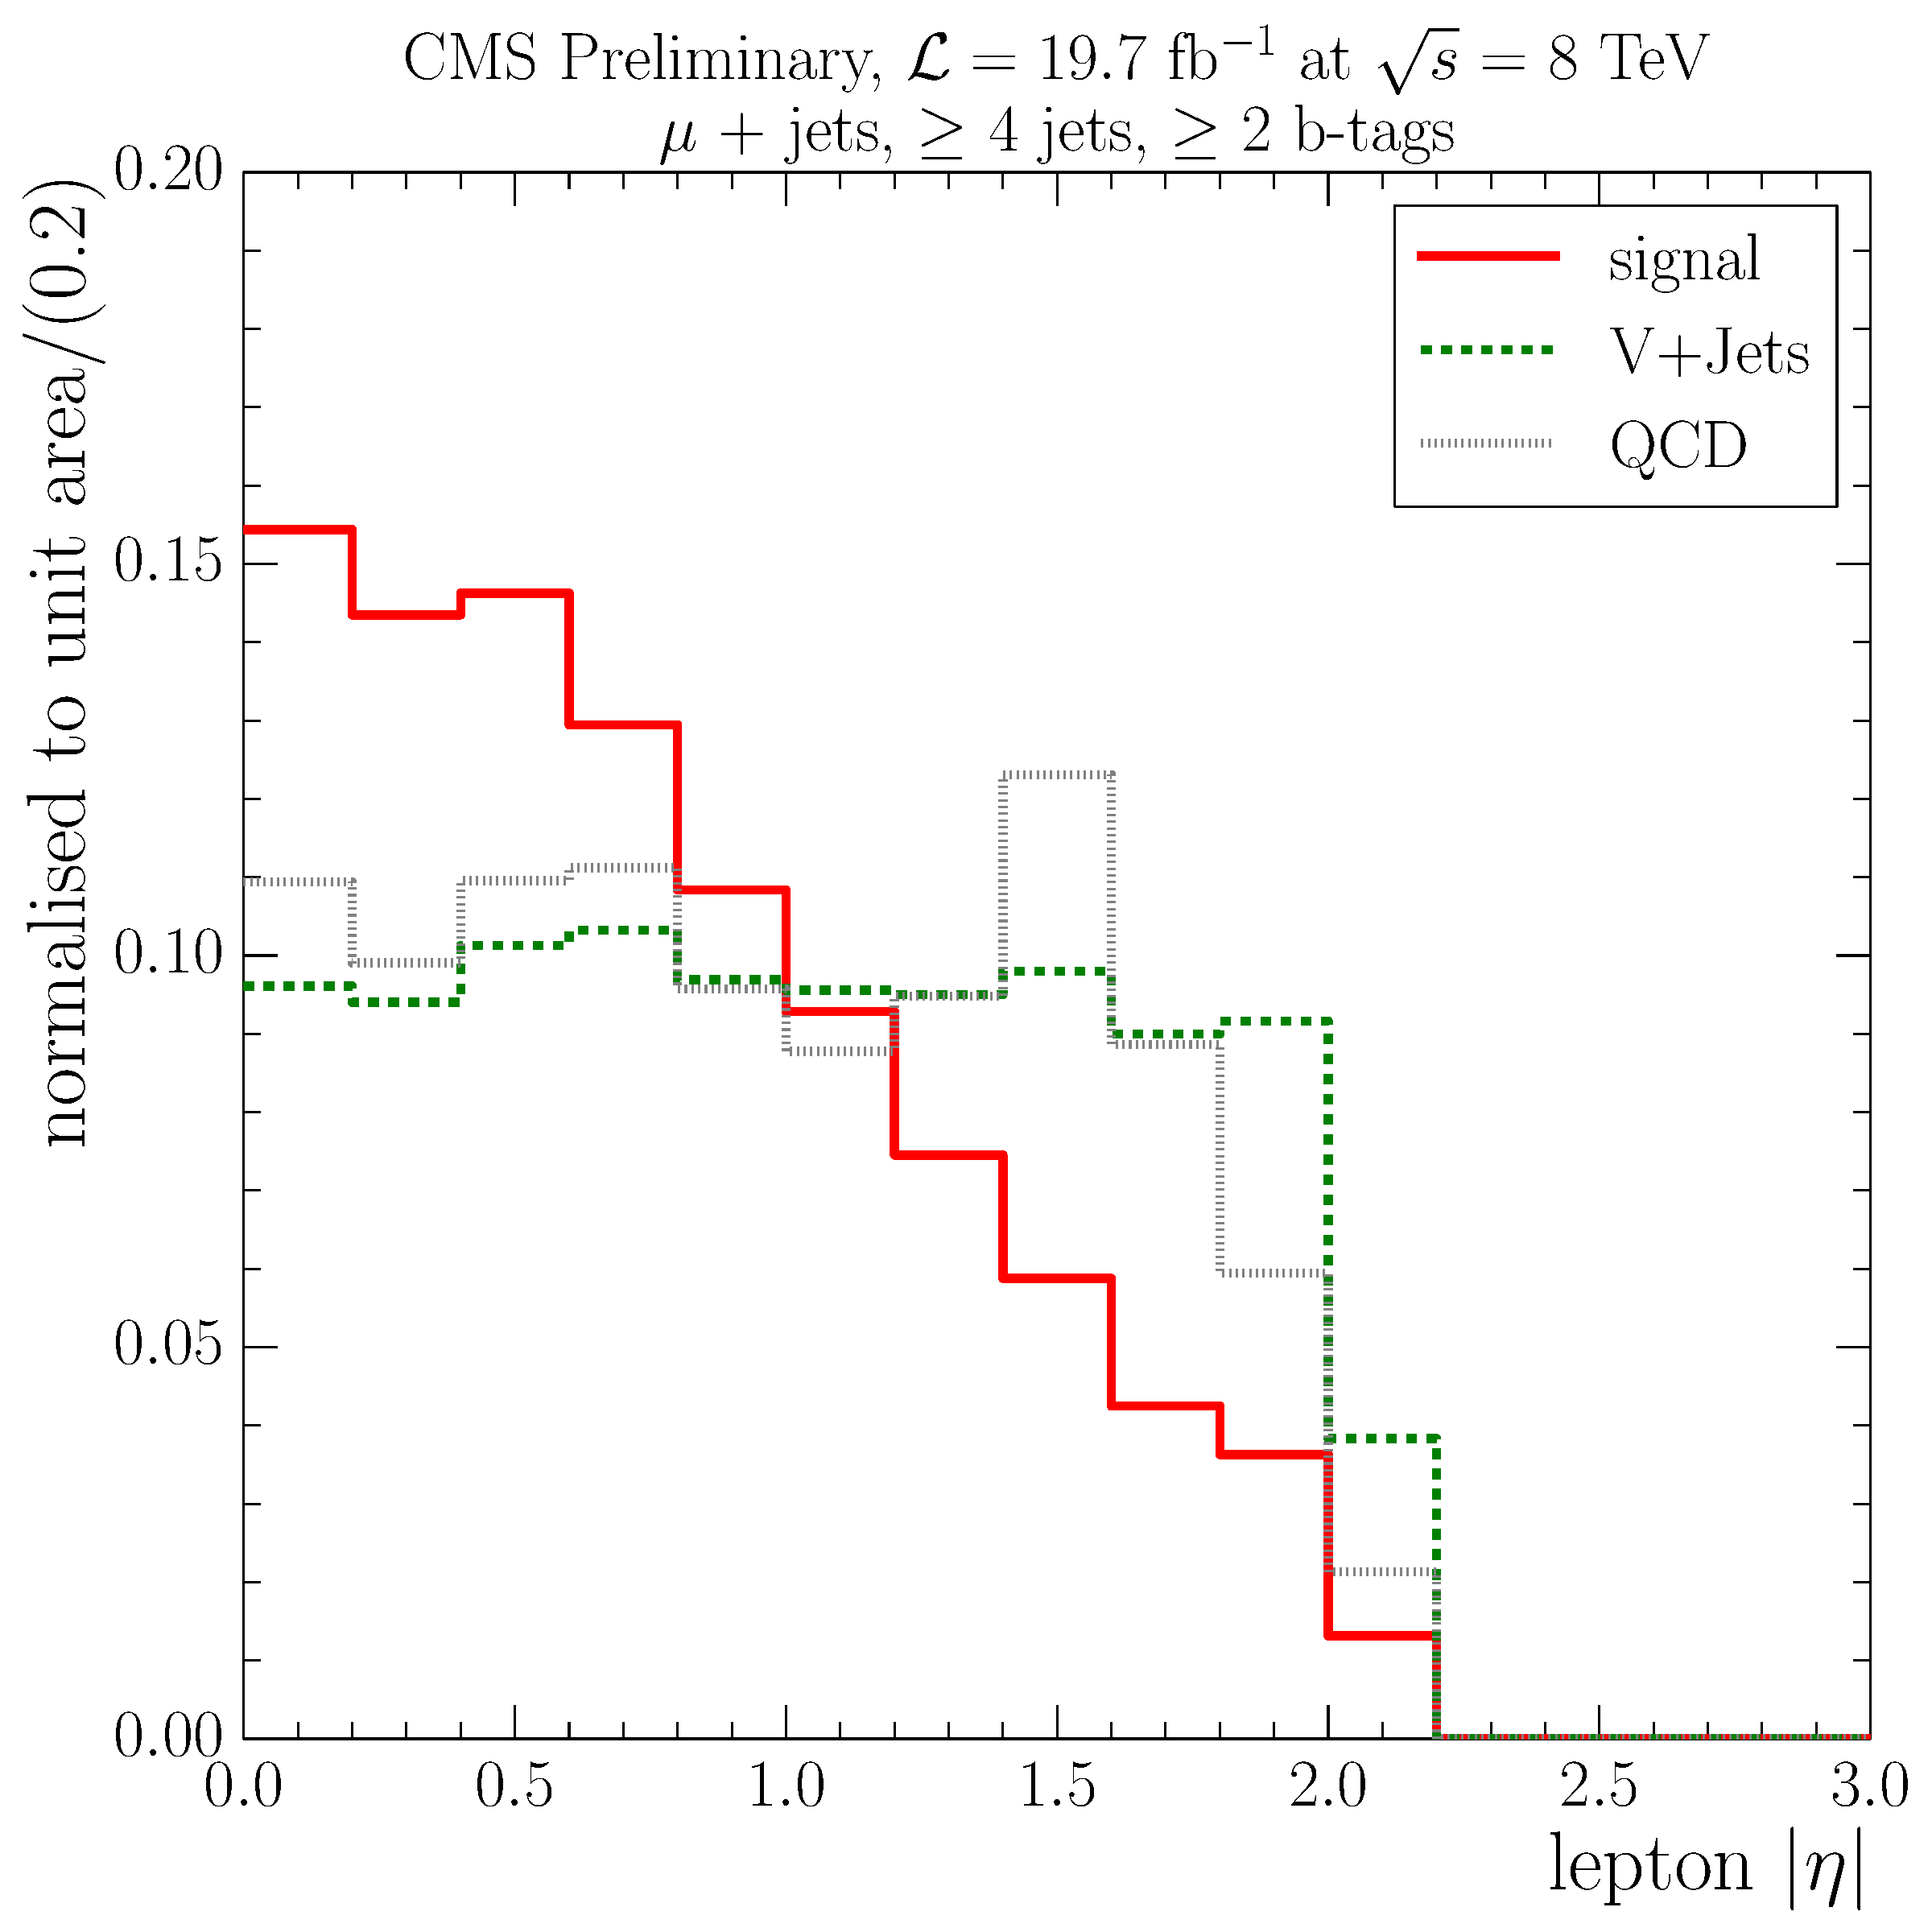
\includegraphics[width=0.3\textwidth]{measurement/MET/central/fit_templates/muon_templates_bin_45-70}}\\
%   	{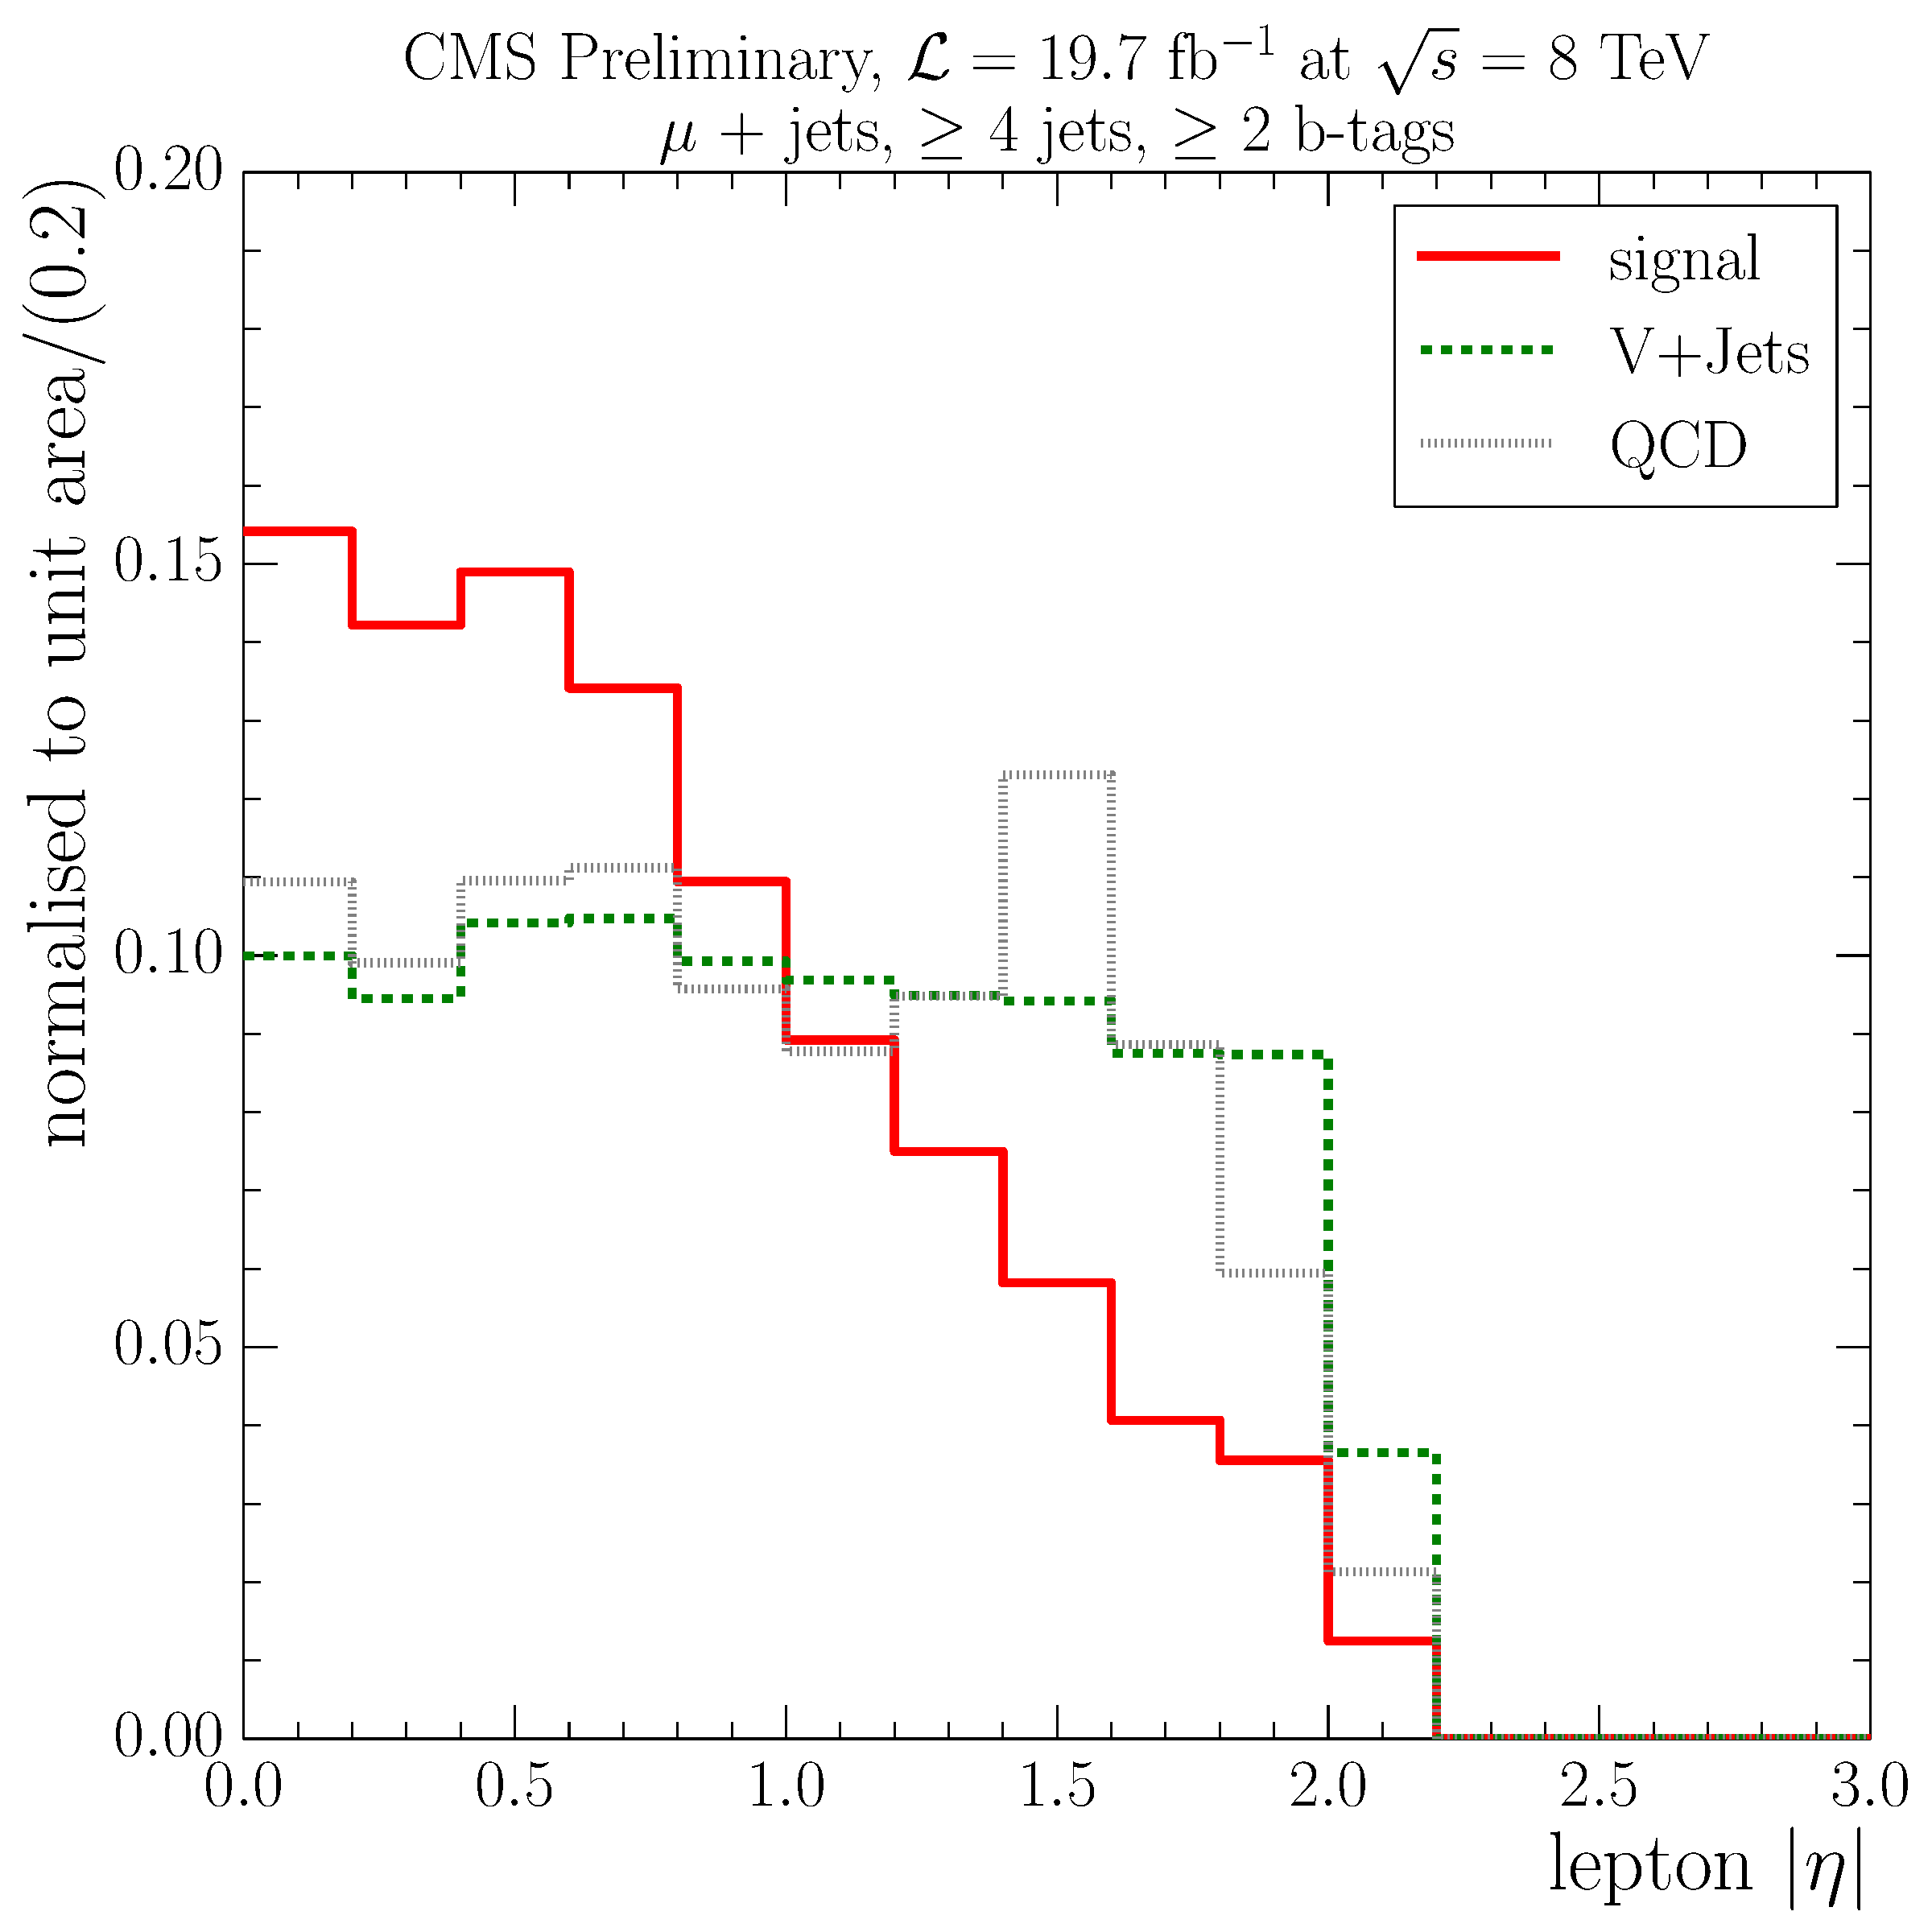
\includegraphics[width=0.3\textwidth]{measurement/MET/central/fit_templates/muon_templates_bin_70-100}}
%   	{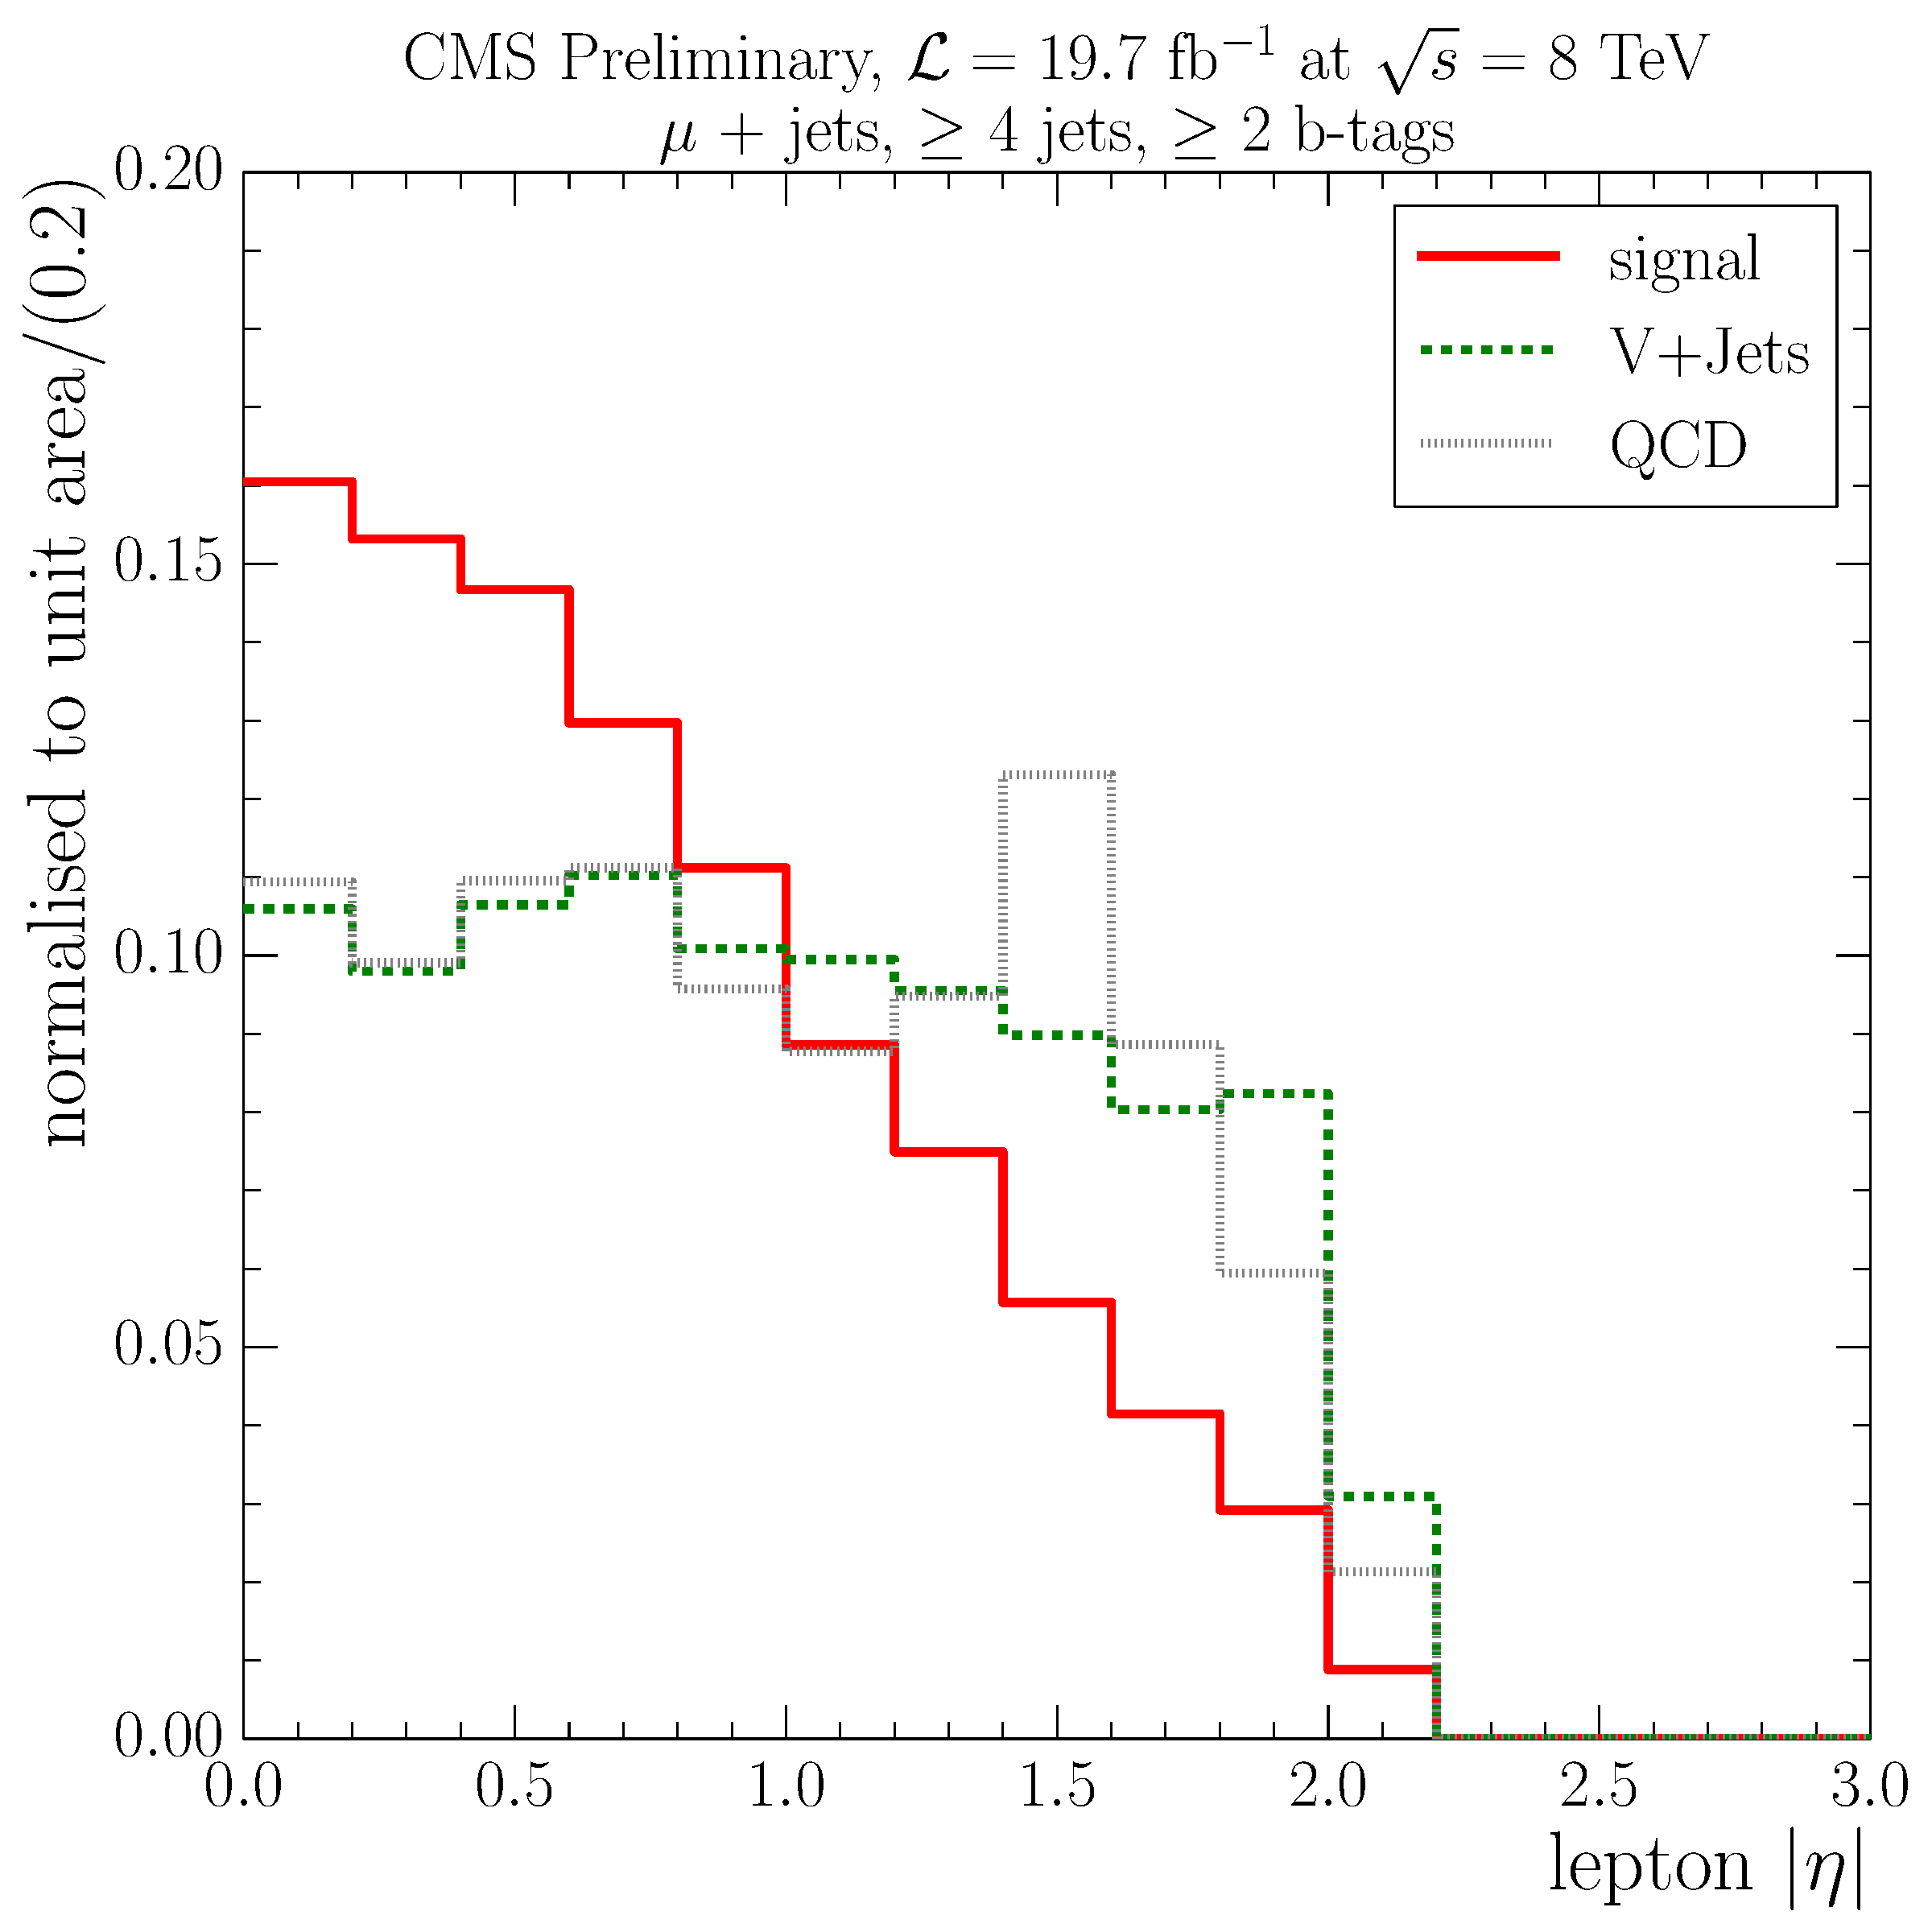
\includegraphics[width=0.3\textwidth]{measurement/MET/central/fit_templates/muon_templates_bin_100-150}}
%   	{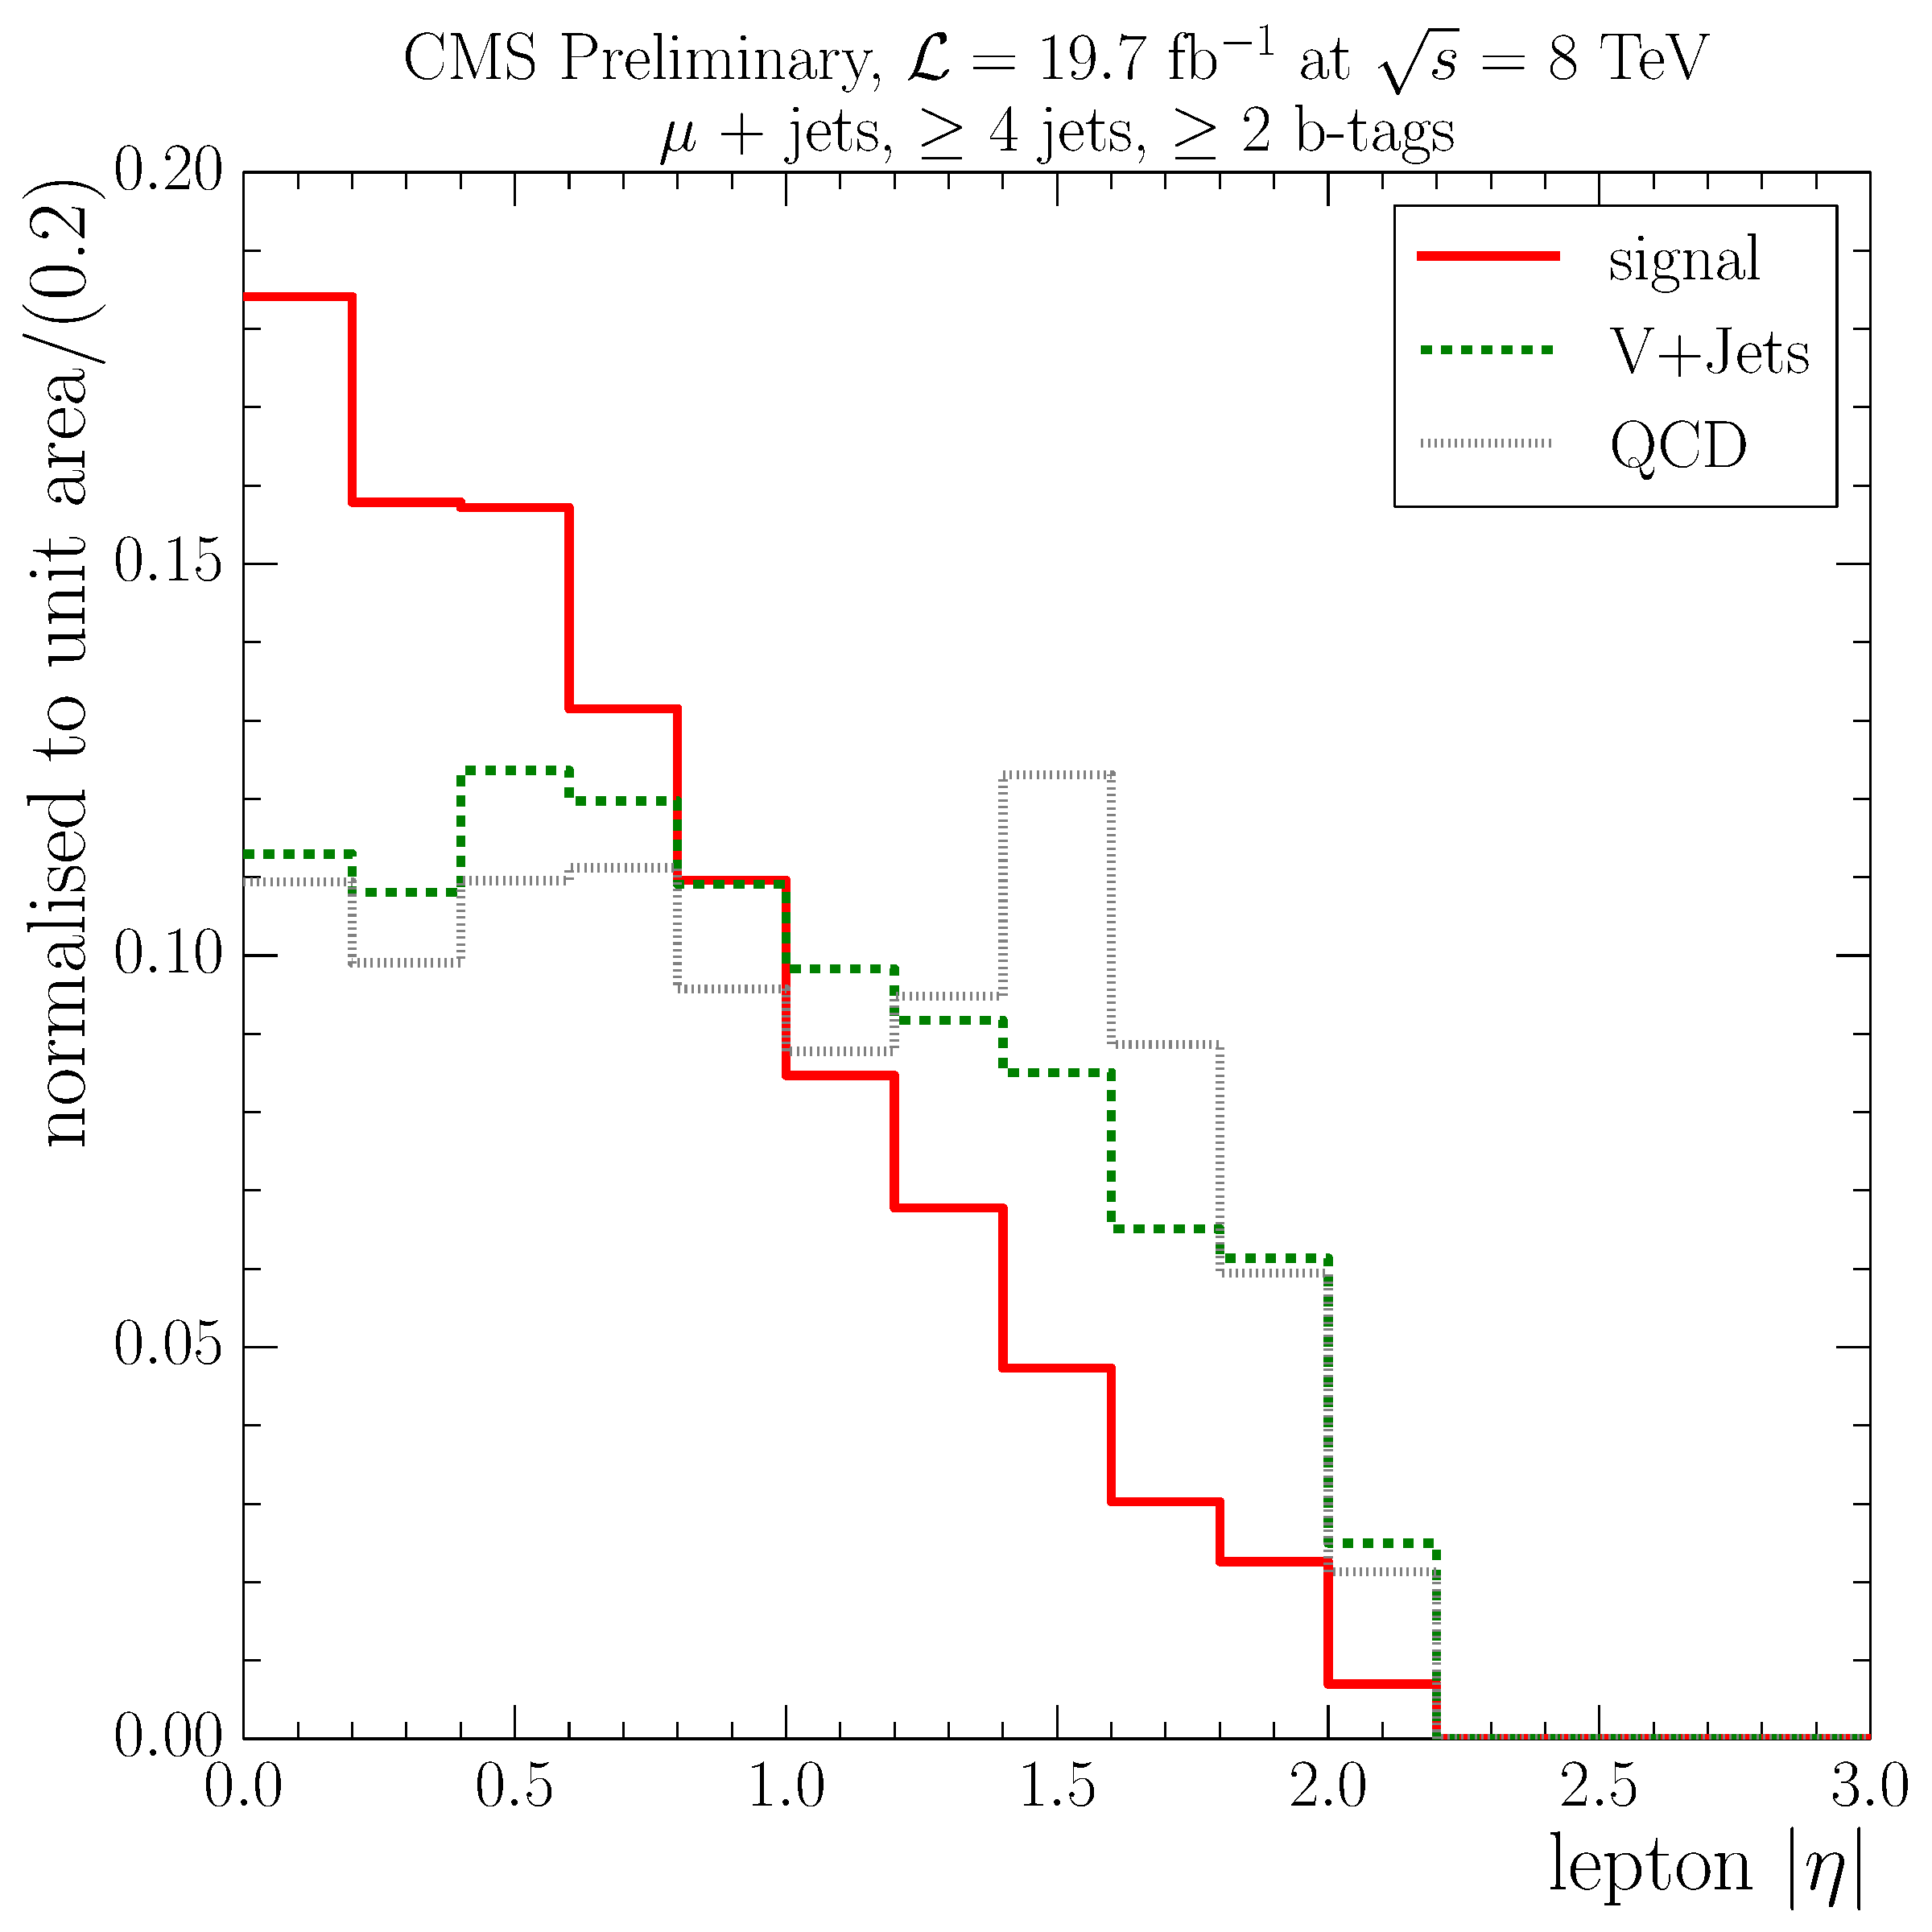
\includegraphics[width=0.3\textwidth]{measurement/MET/central/fit_templates/muon_templates_bin_150-inf}}
%     \caption{Electron $\abs \eta$ templates for the fit in different bins of
%     \MET, from top left to bottom right: \SIrange{0}{25}{\GeV},
%     \SIrange{25}{45}{\GeV},
%     \SIrange{45}{70}{\GeV}, \SIrange{70}{100}{\GeV}, \SIrange{100}{150}{\GeV} and $\geq \SI{150}{\GeV}$.}
%     \label{fig:fit_results_MET_muon}
% \end{figure}

\centering
\section*{\HT variable}

\begin{figure}[!htbp]
	\centering
  	{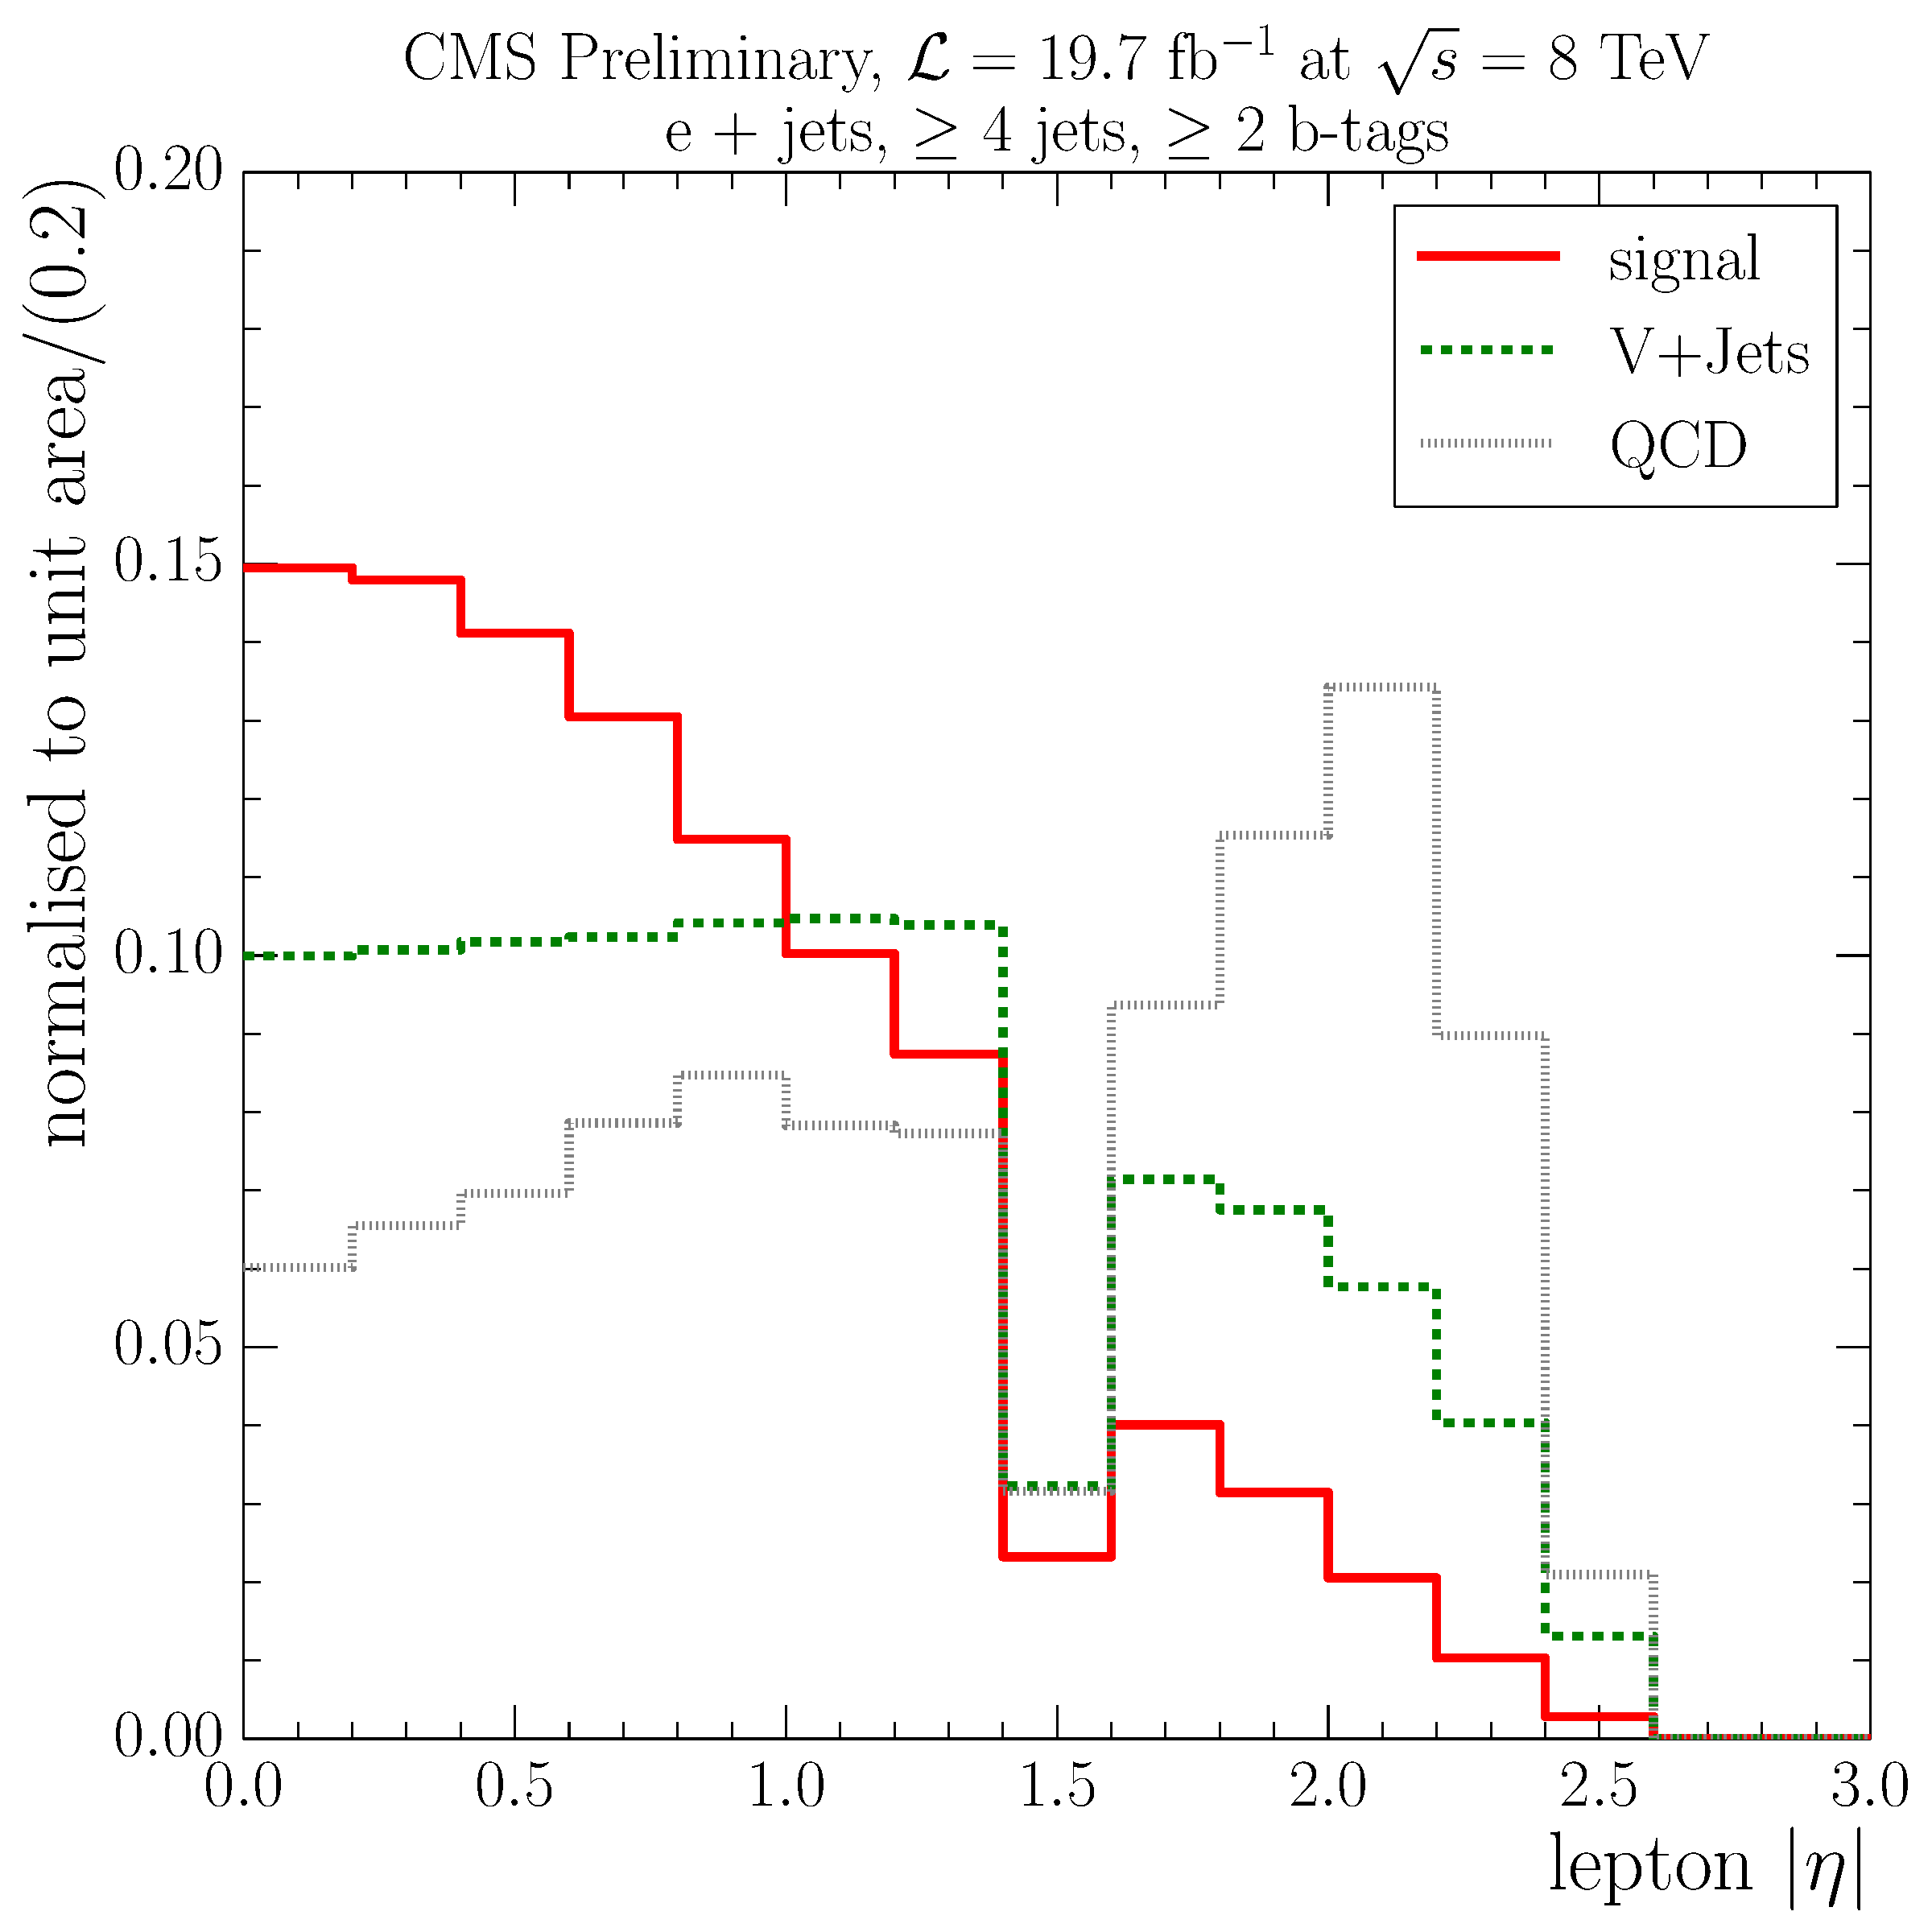
\includegraphics[width=0.3\textwidth]{measurement/HT/central/fit_templates/electron_templates_bin_0-240}}
  	{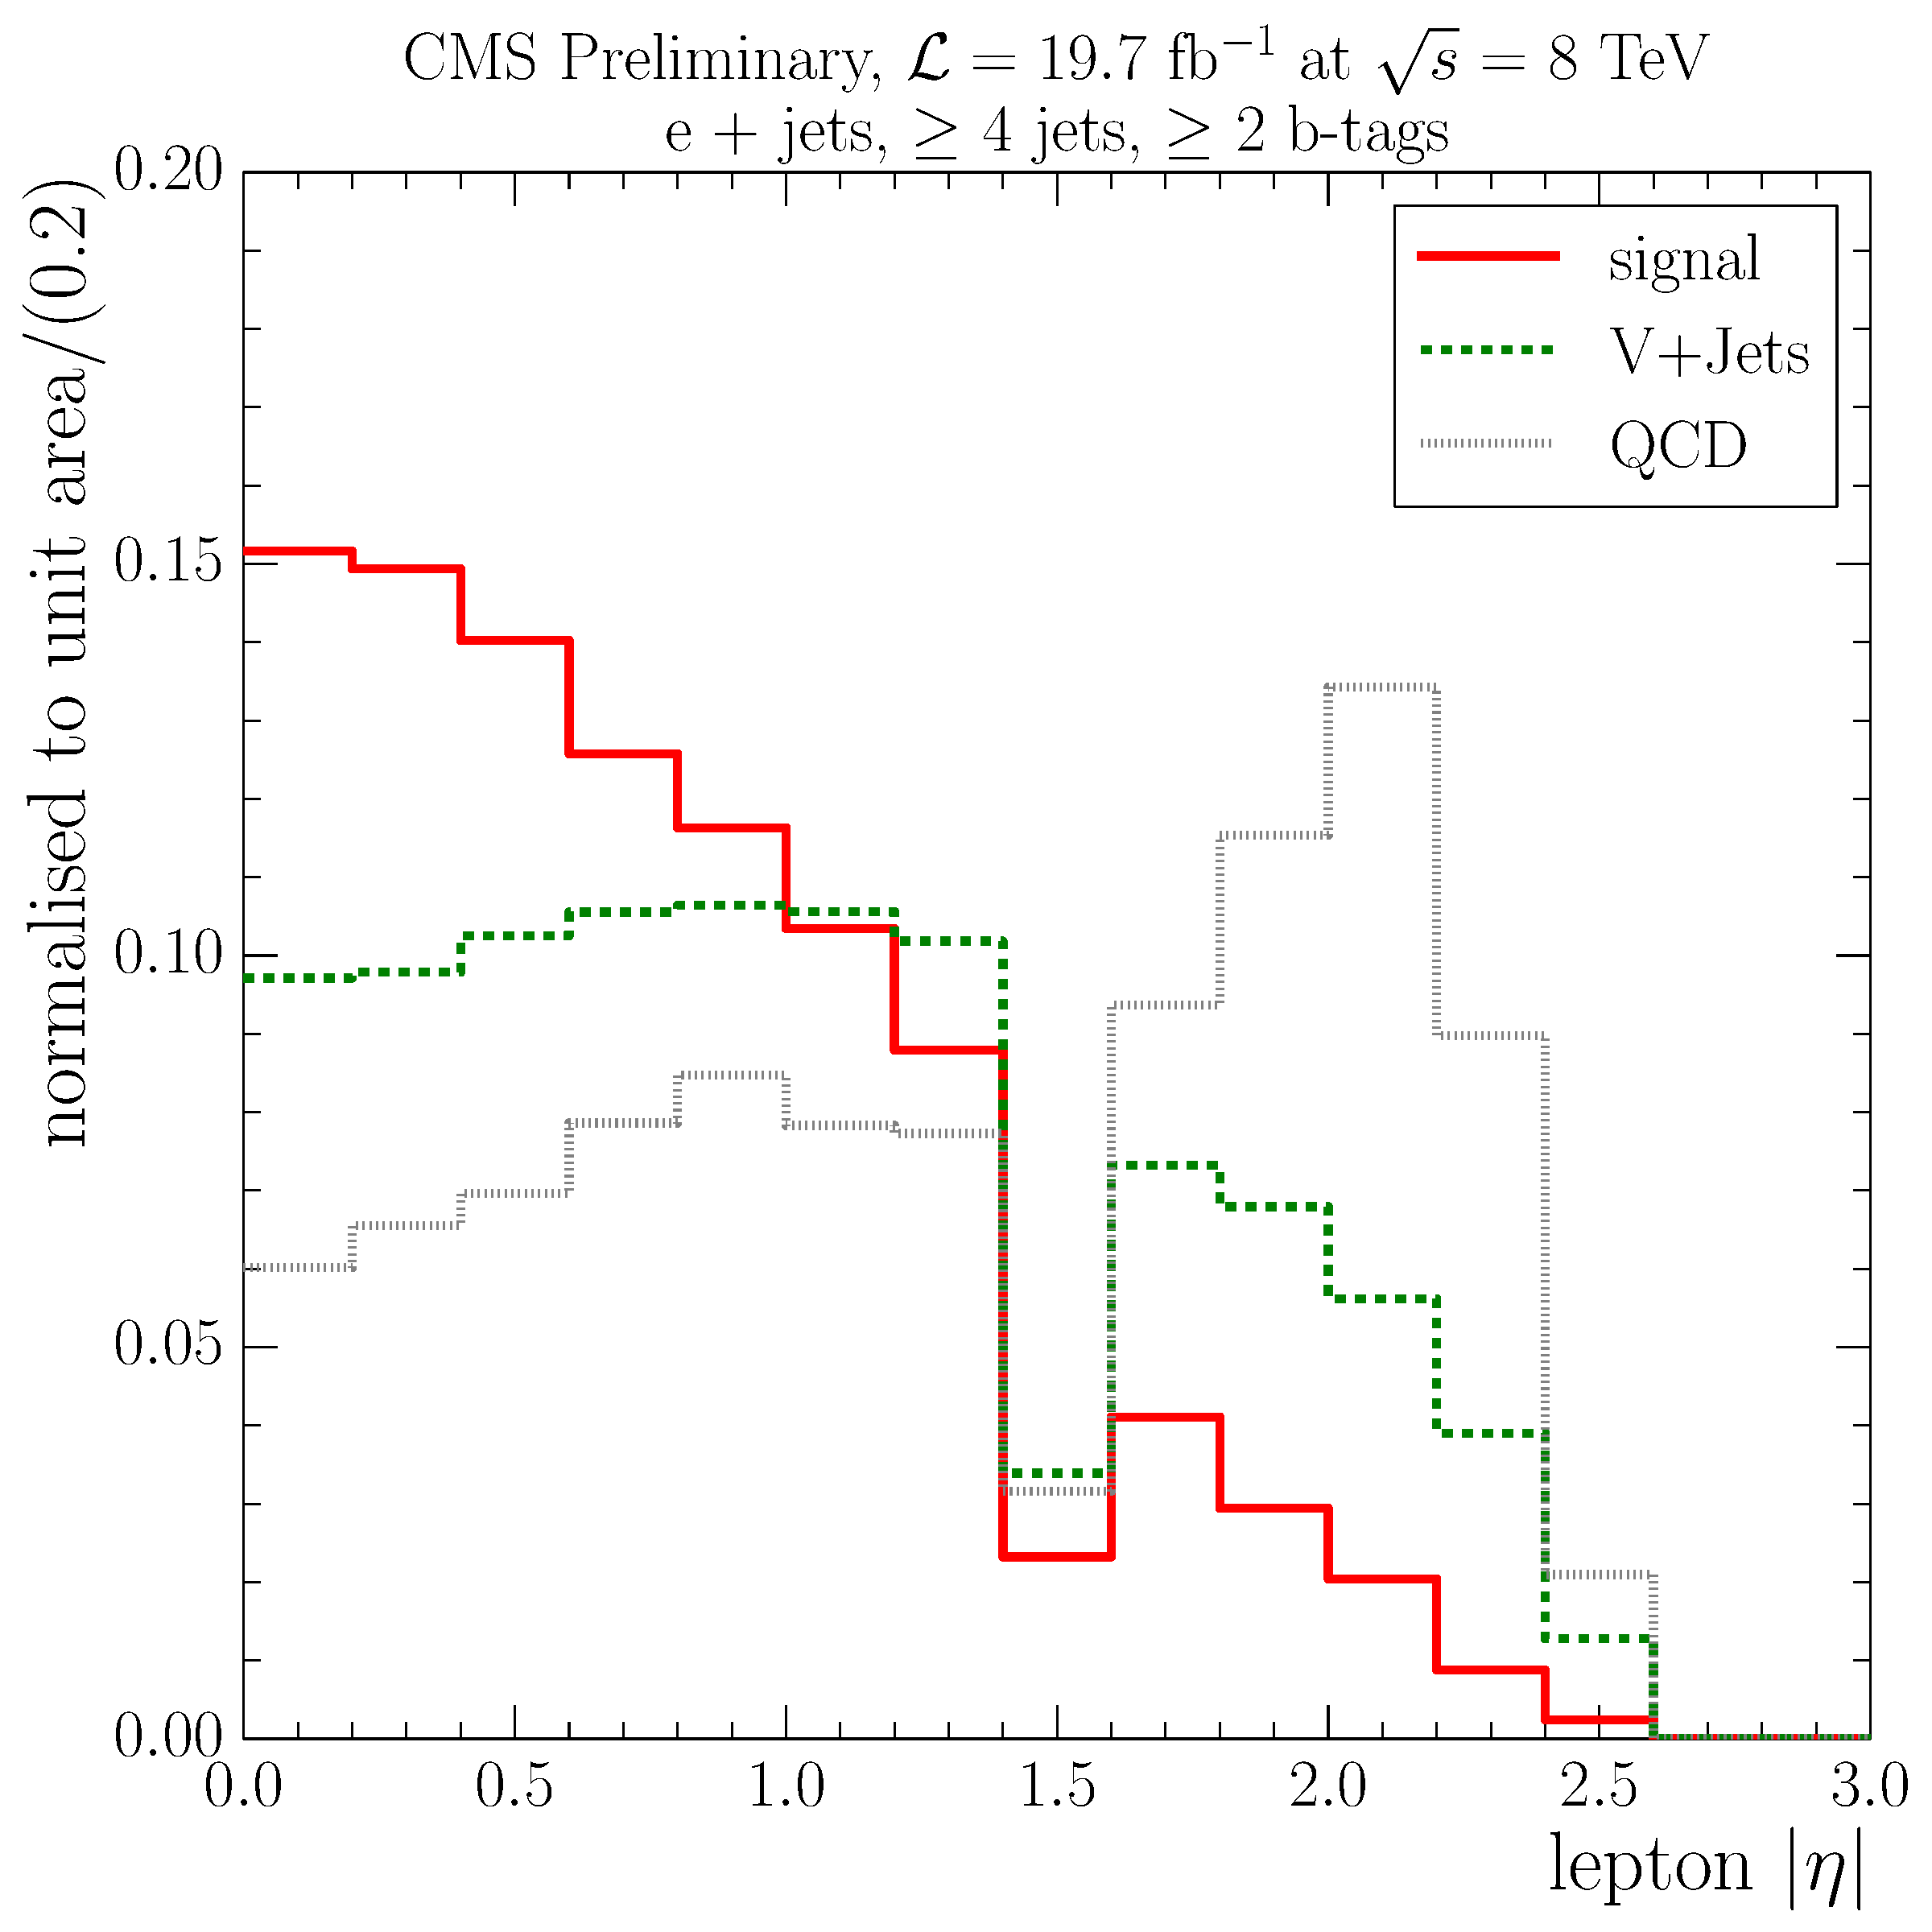
\includegraphics[width=0.3\textwidth]{measurement/HT/central/fit_templates/electron_templates_bin_240-280}}
  	{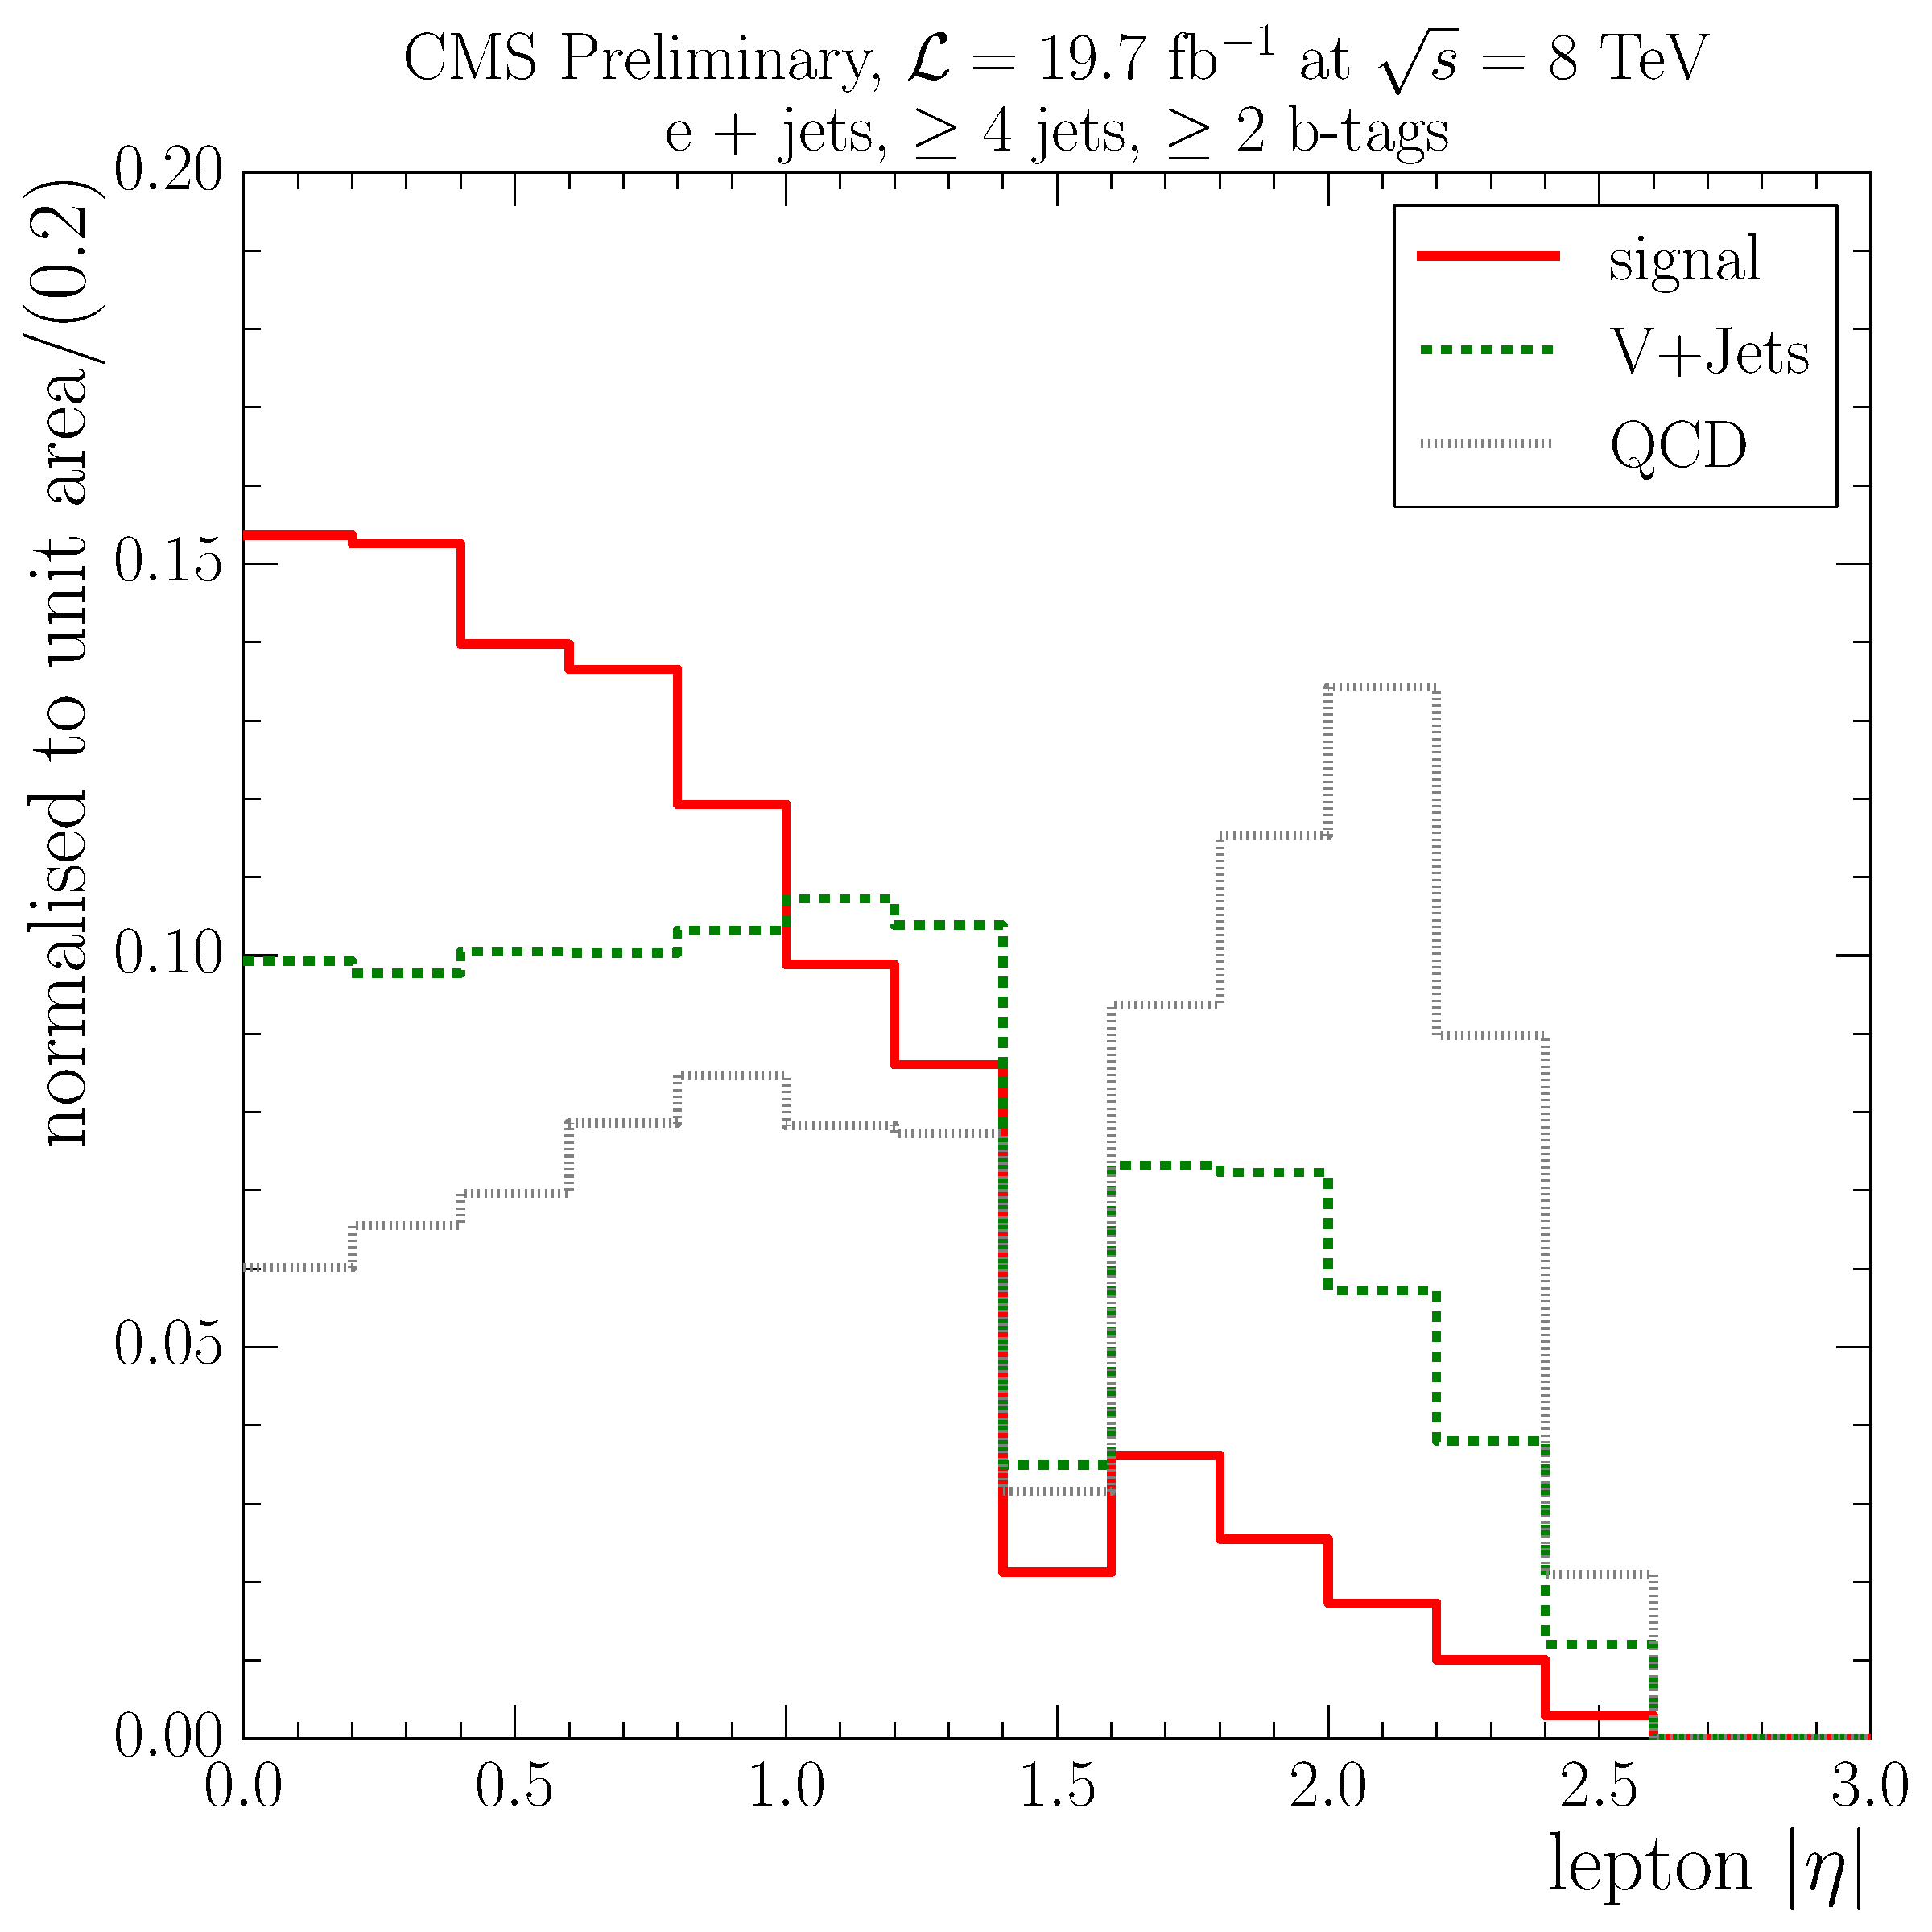
\includegraphics[width=0.3\textwidth]{measurement/HT/central/fit_templates/electron_templates_bin_280-330}}\\
  	{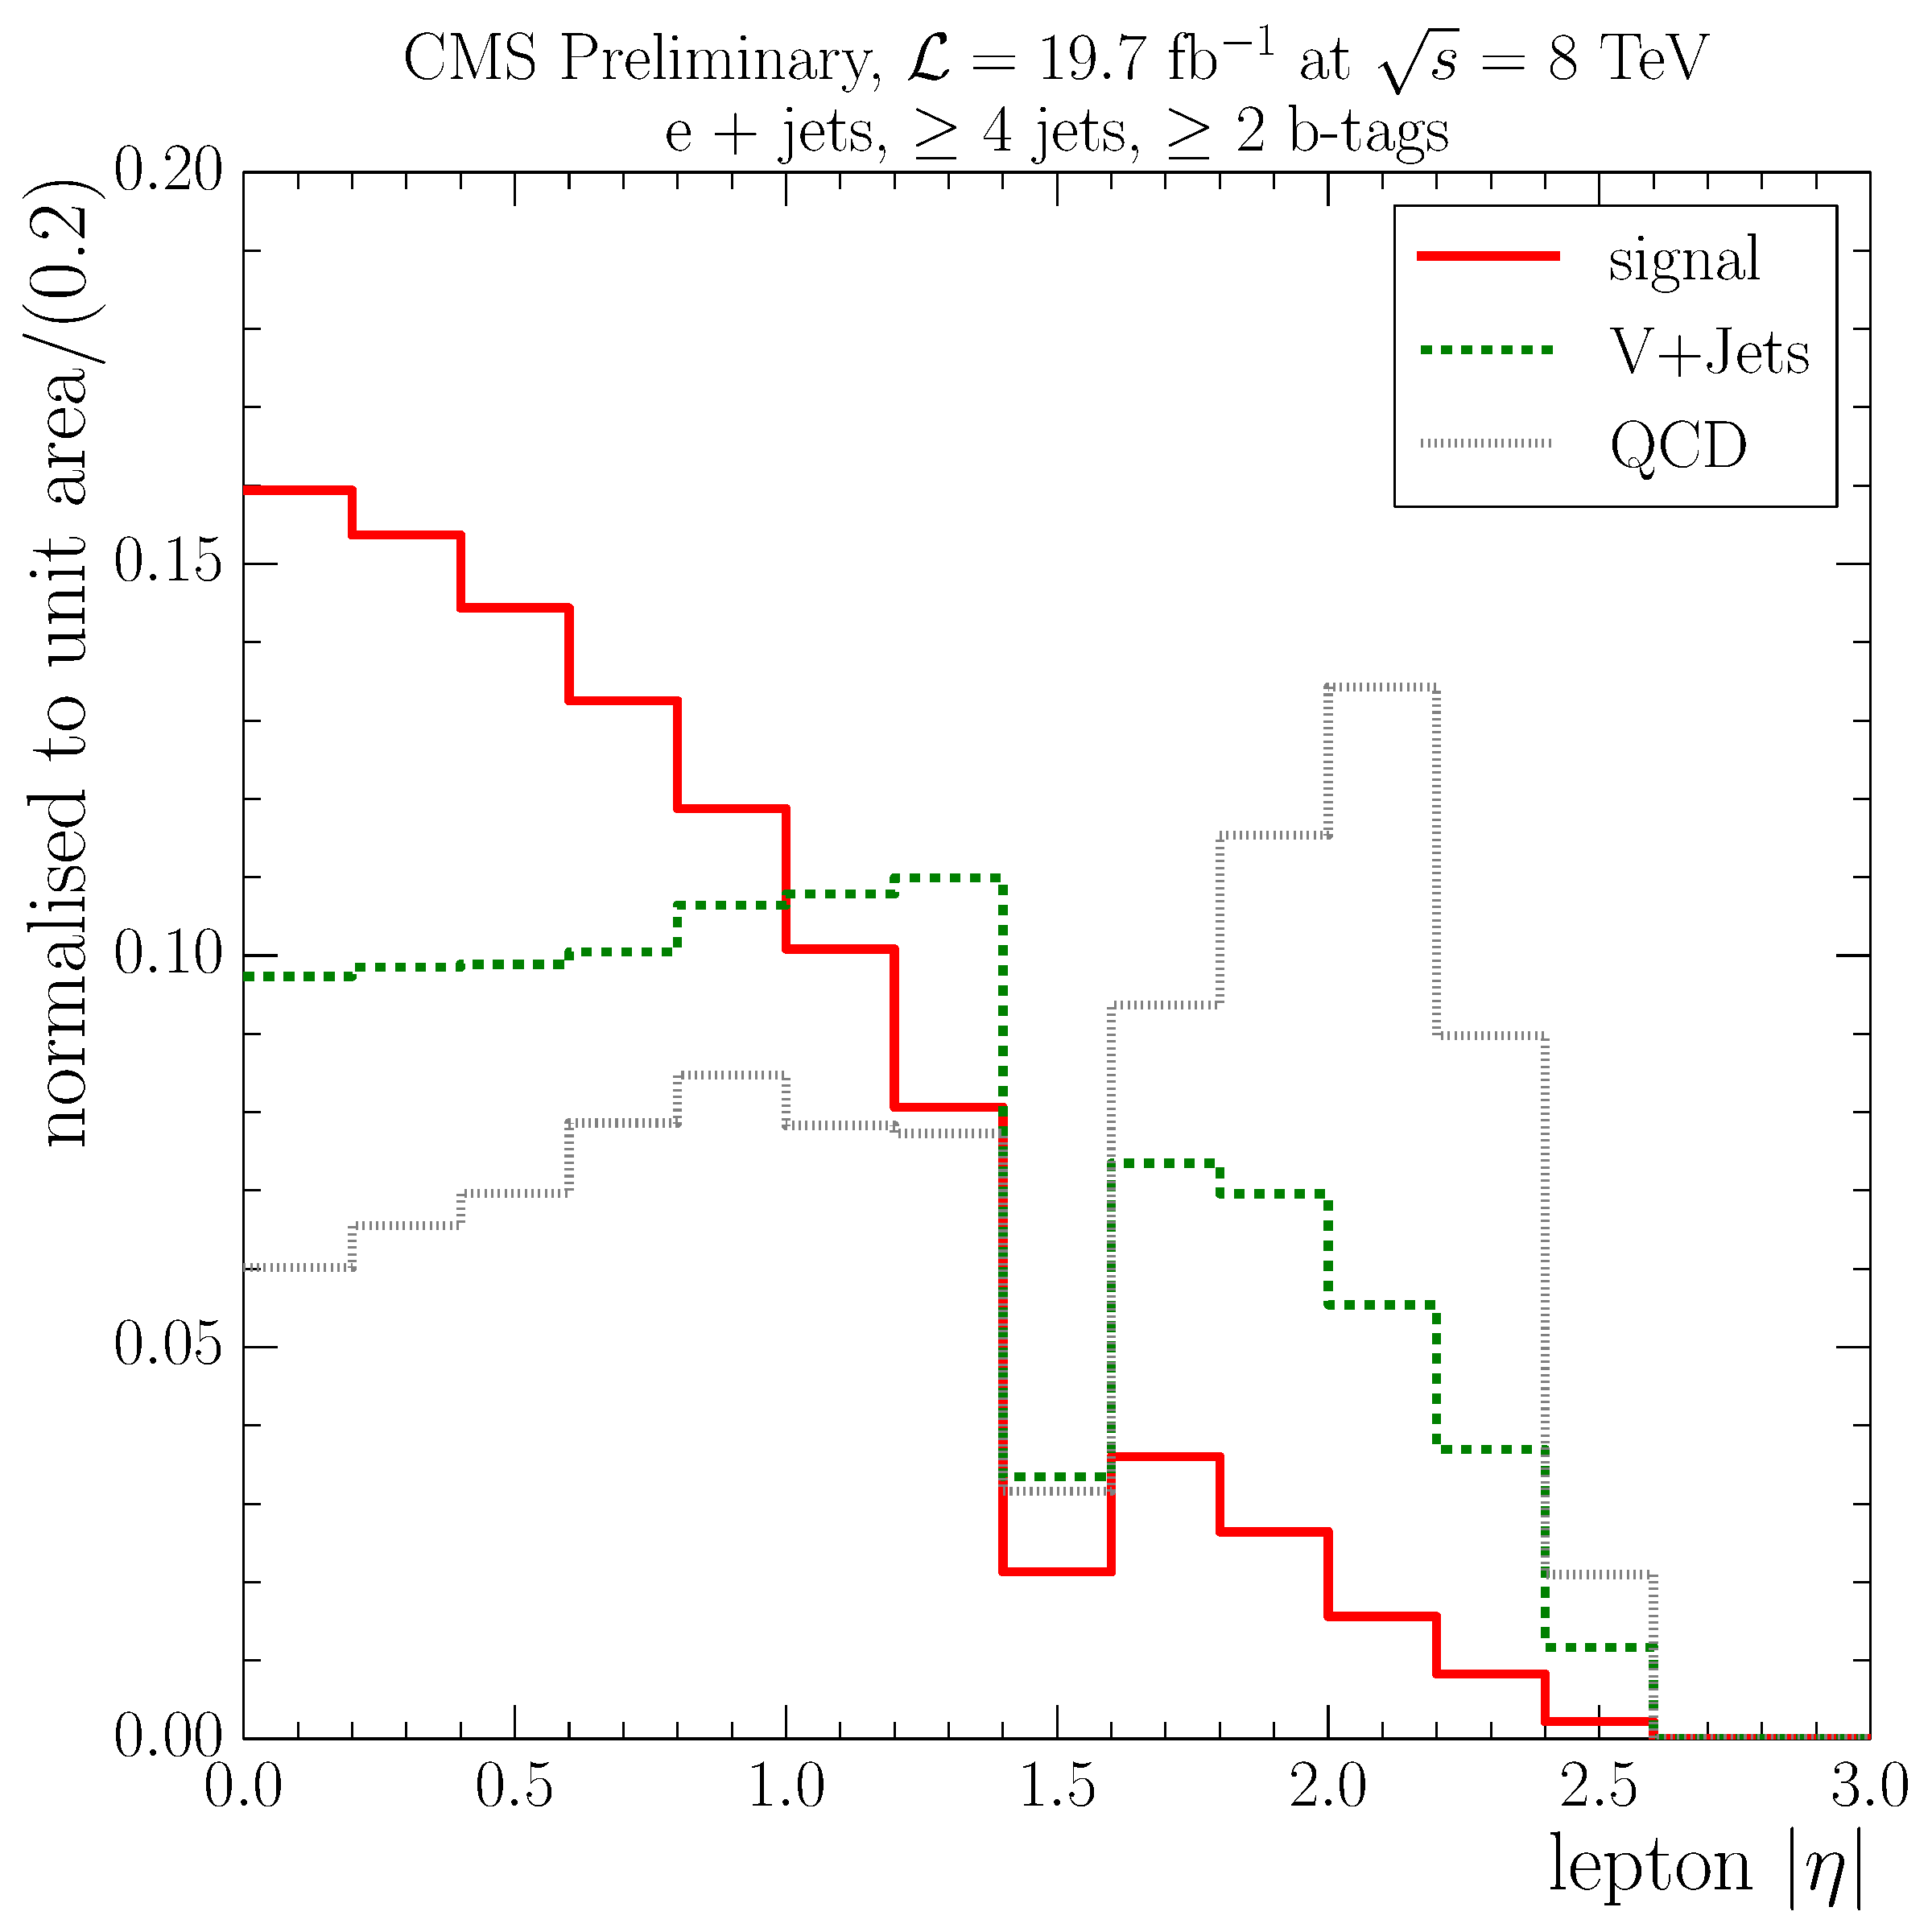
\includegraphics[width=0.3\textwidth]{measurement/HT/central/fit_templates/electron_templates_bin_330-380}}
  	{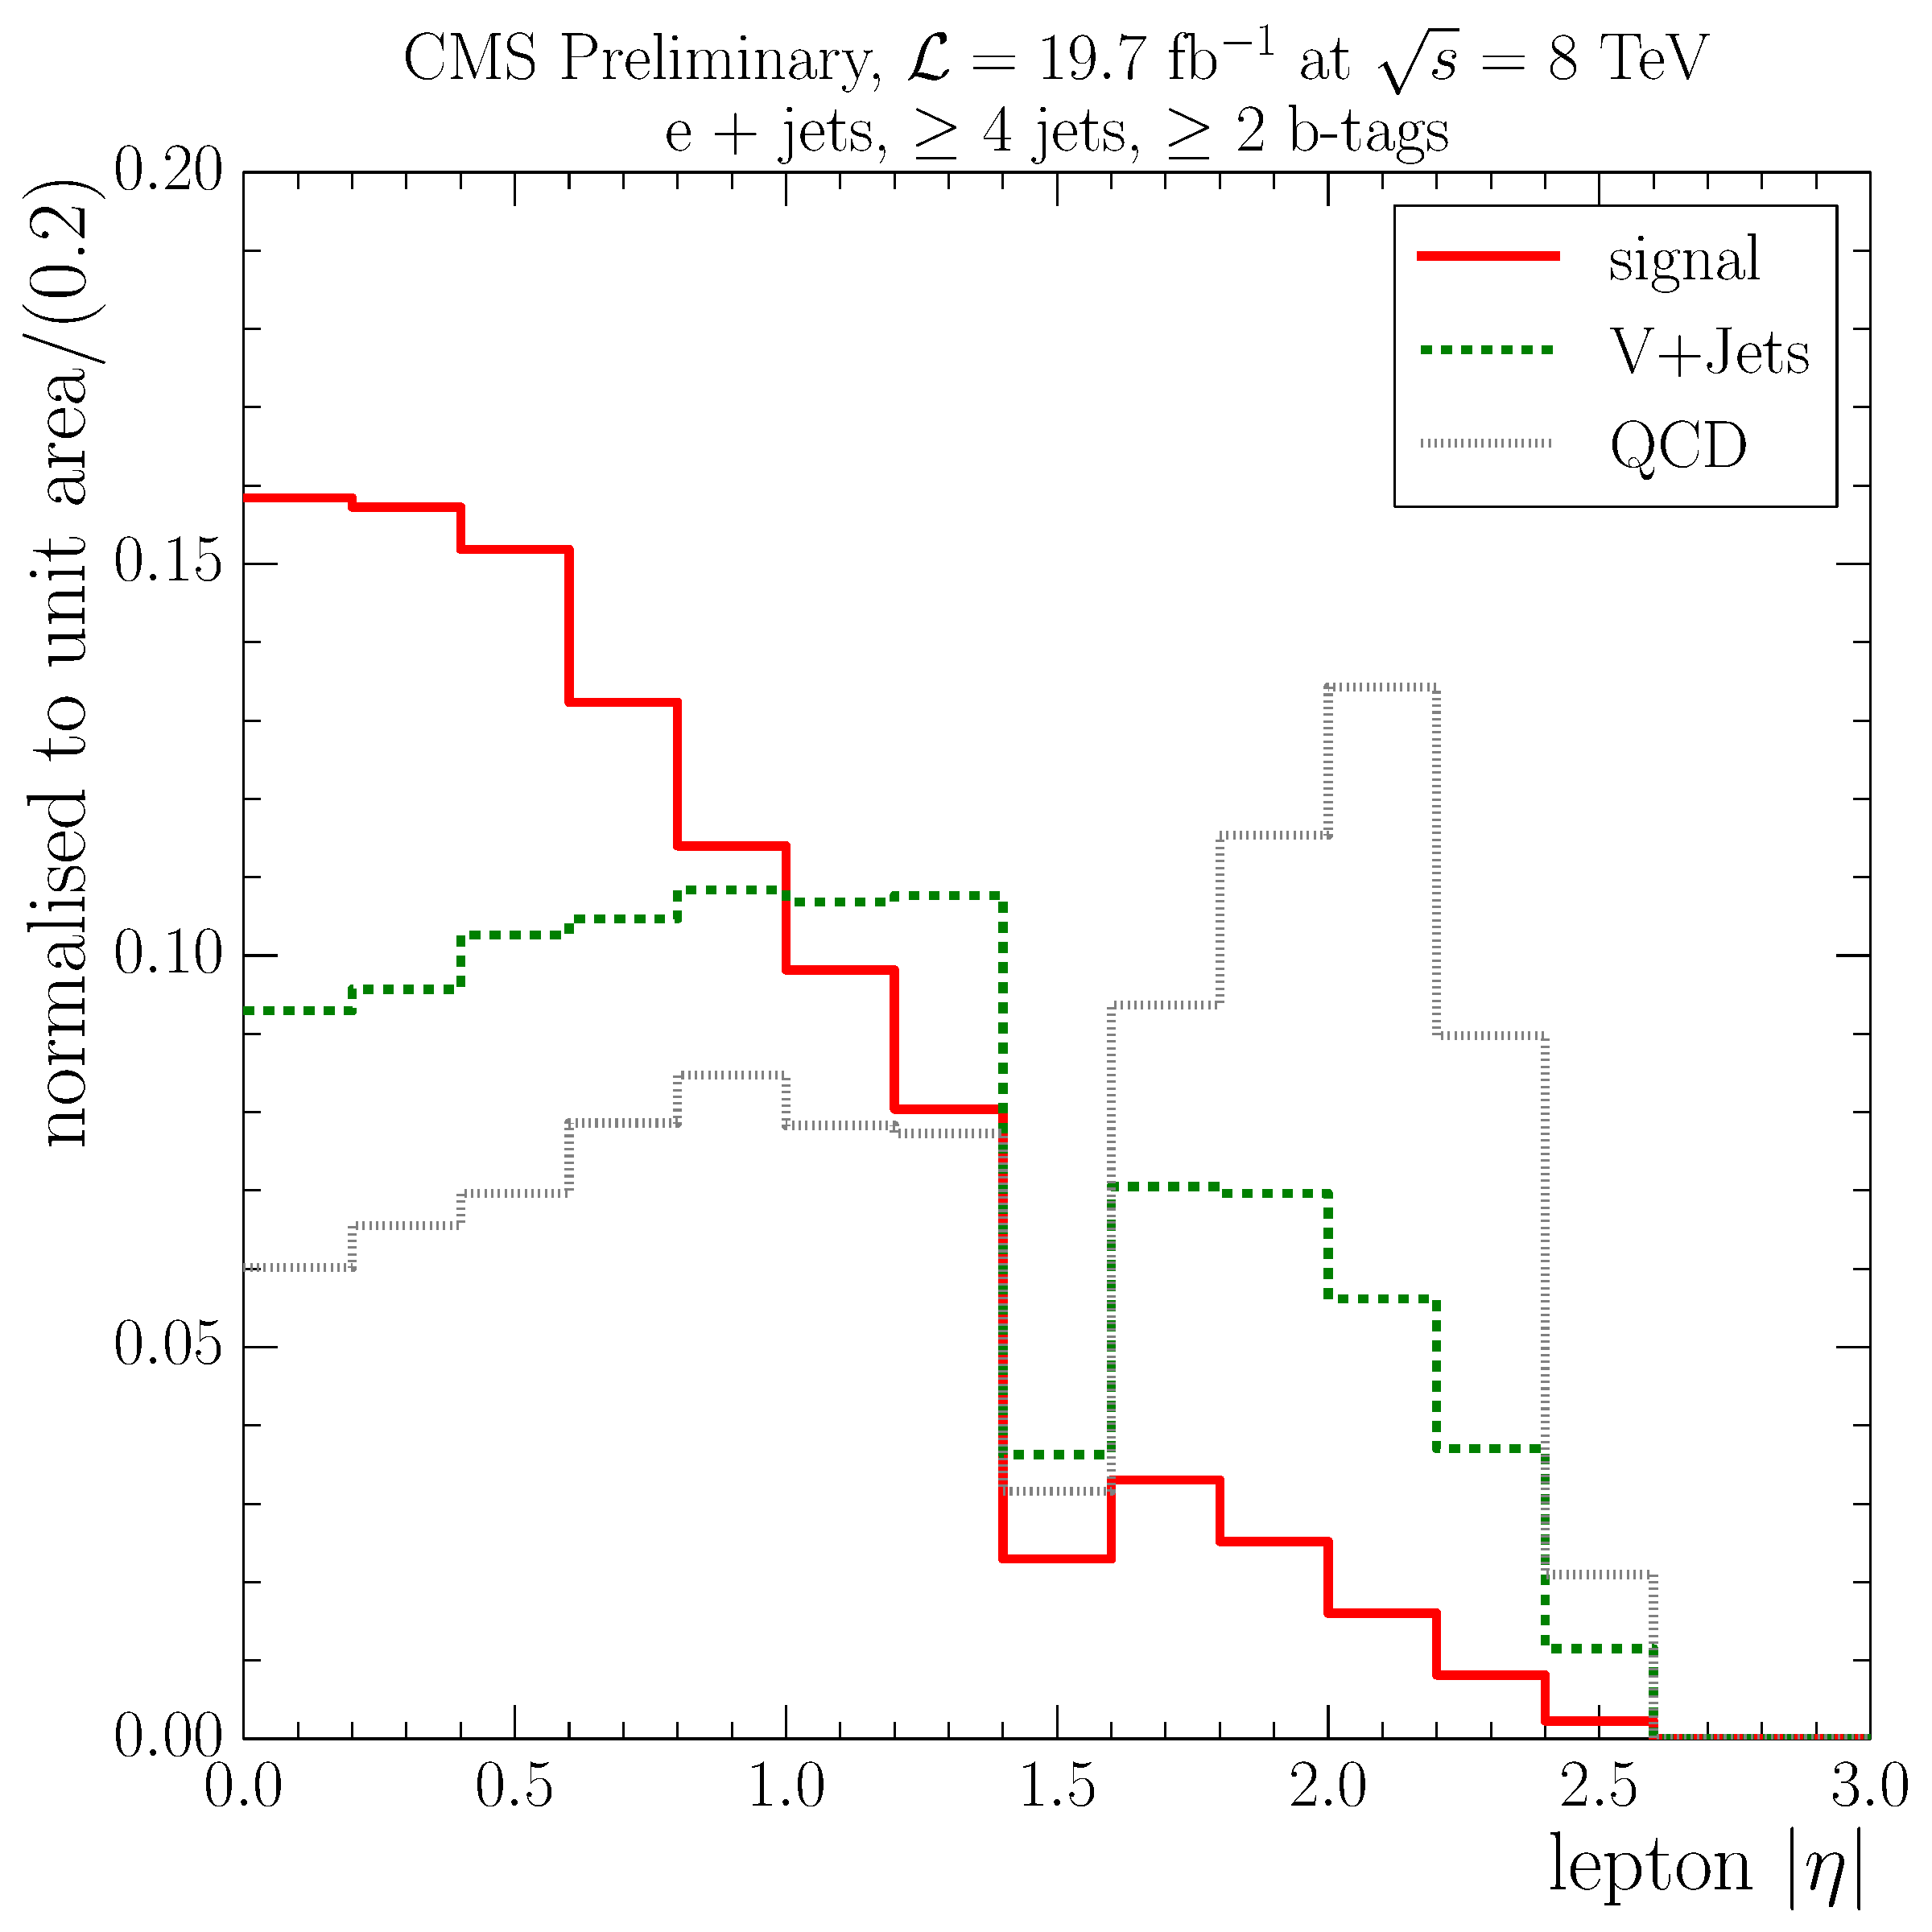
\includegraphics[width=0.3\textwidth]{measurement/HT/central/fit_templates/electron_templates_bin_380-450}}
  	{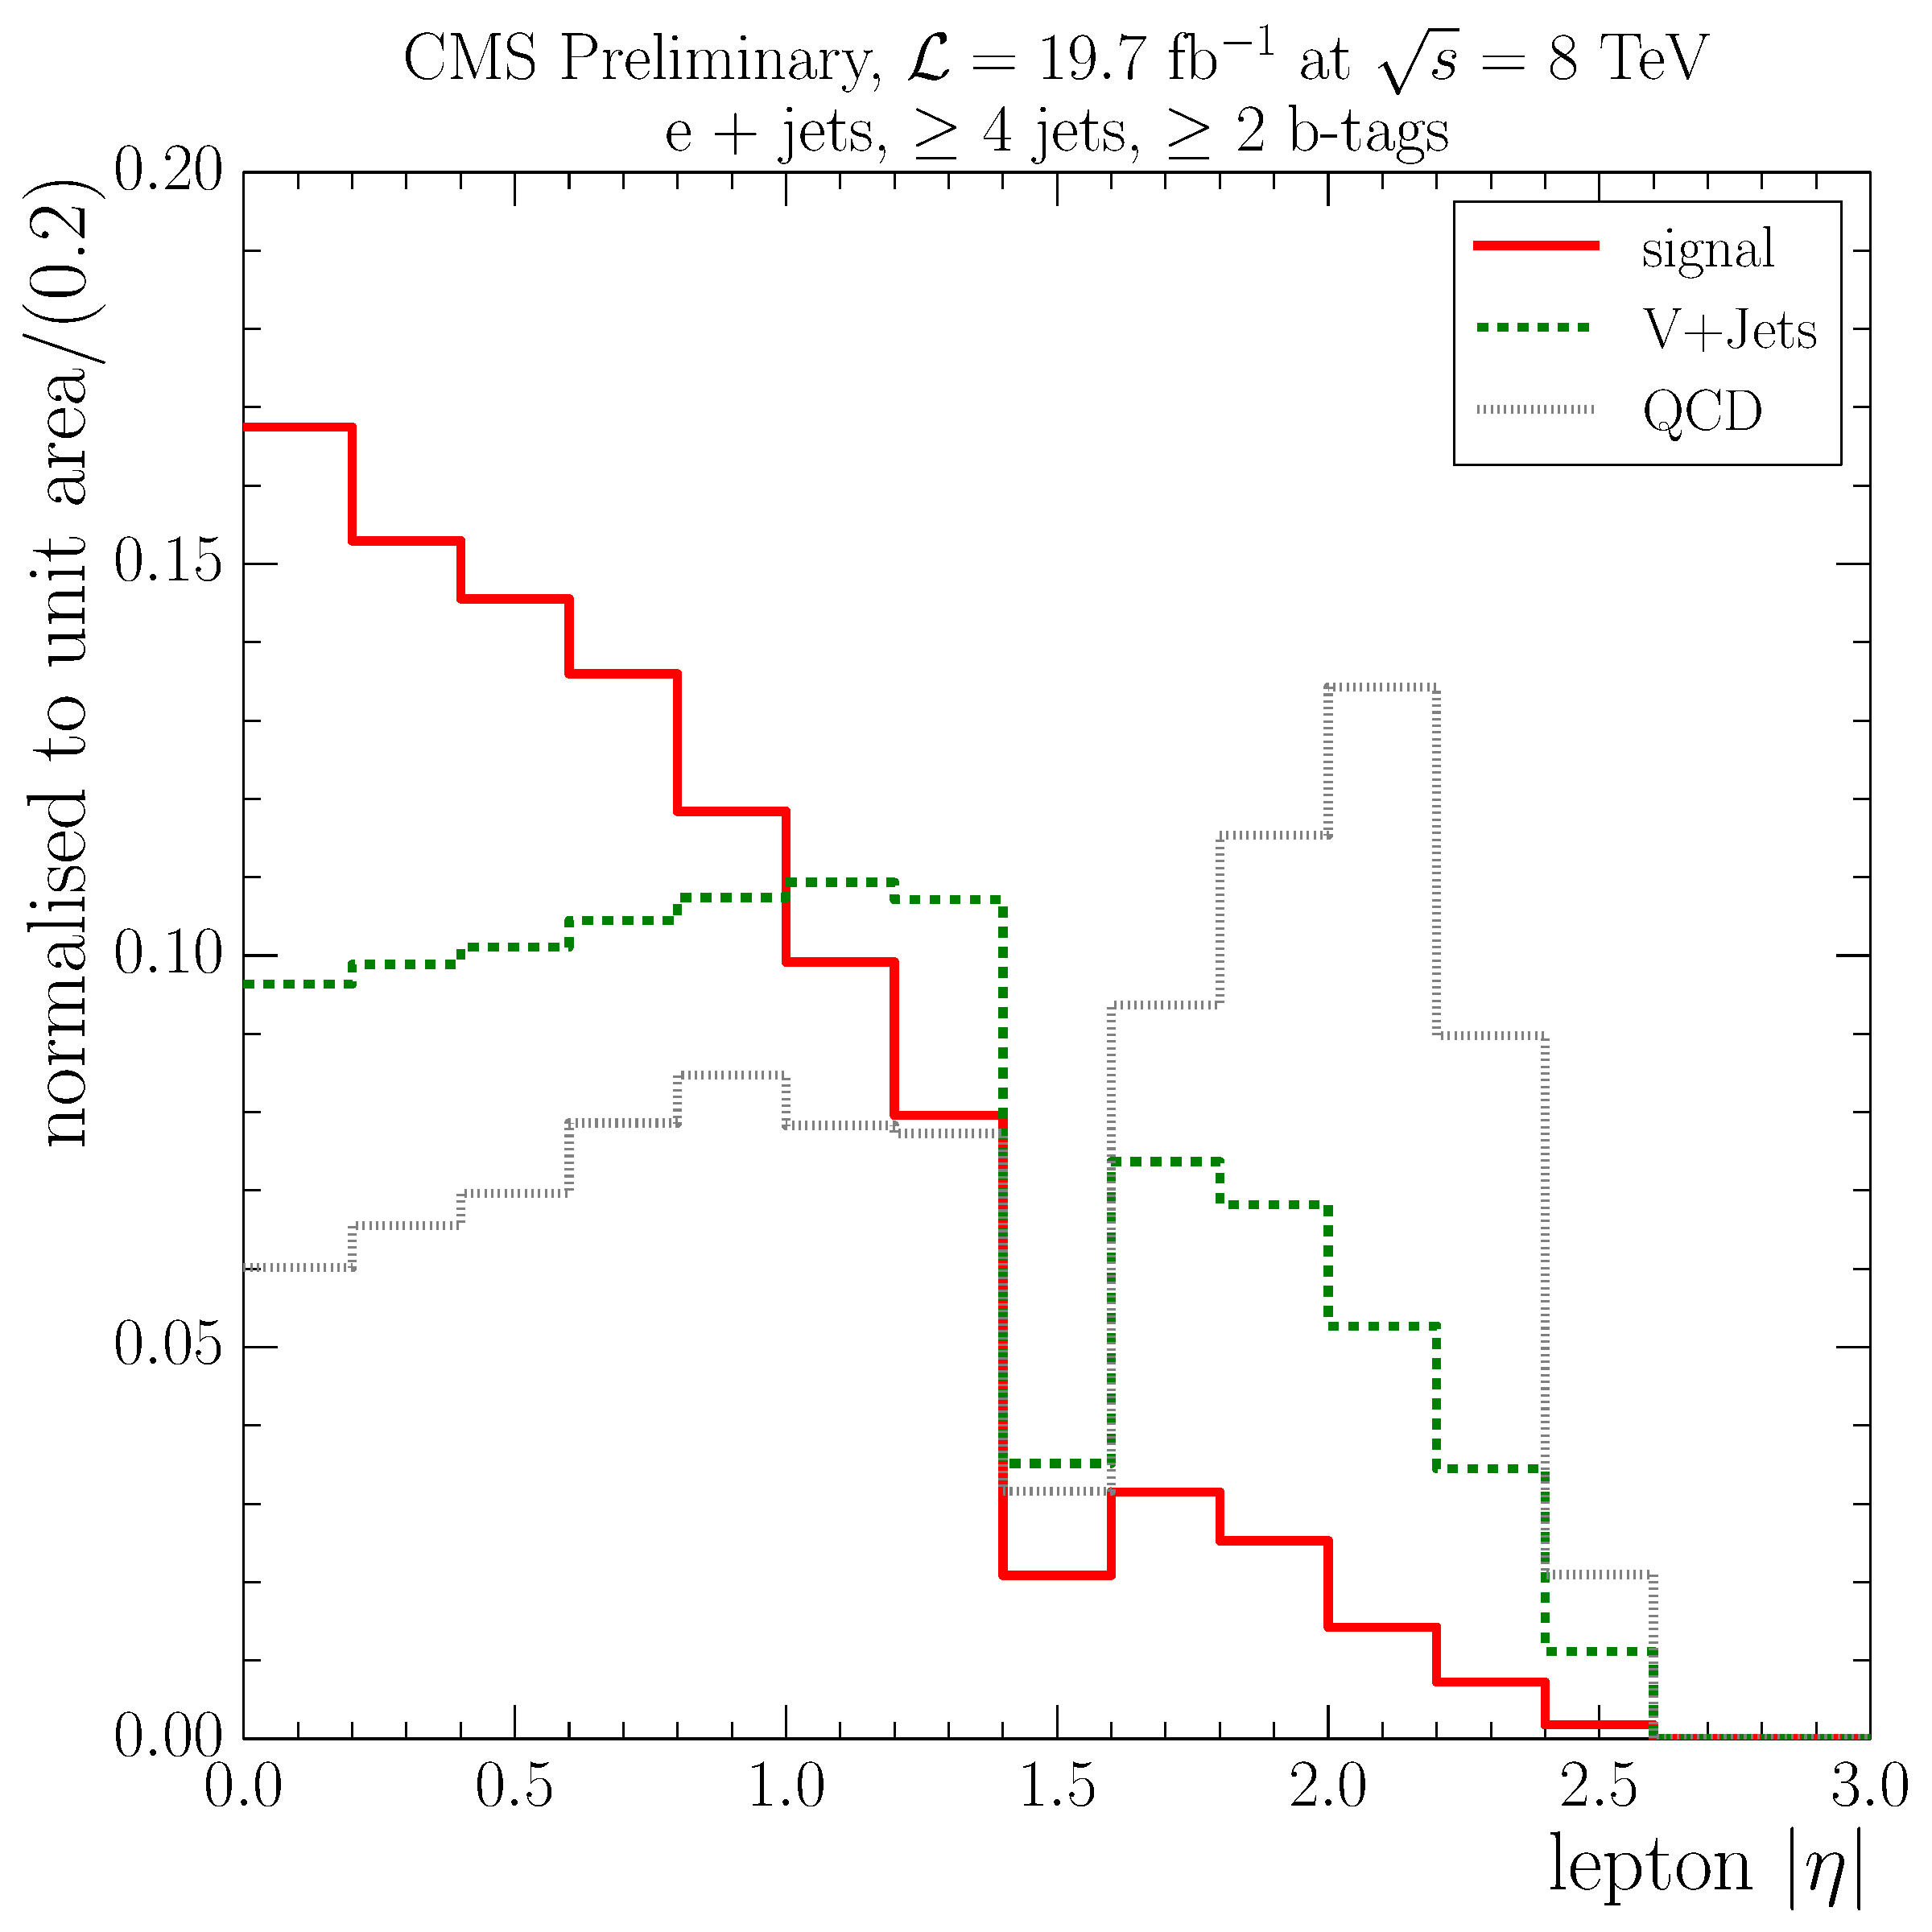
\includegraphics[width=0.3\textwidth]{measurement/HT/central/fit_templates/electron_templates_bin_450-600}}\\
  	{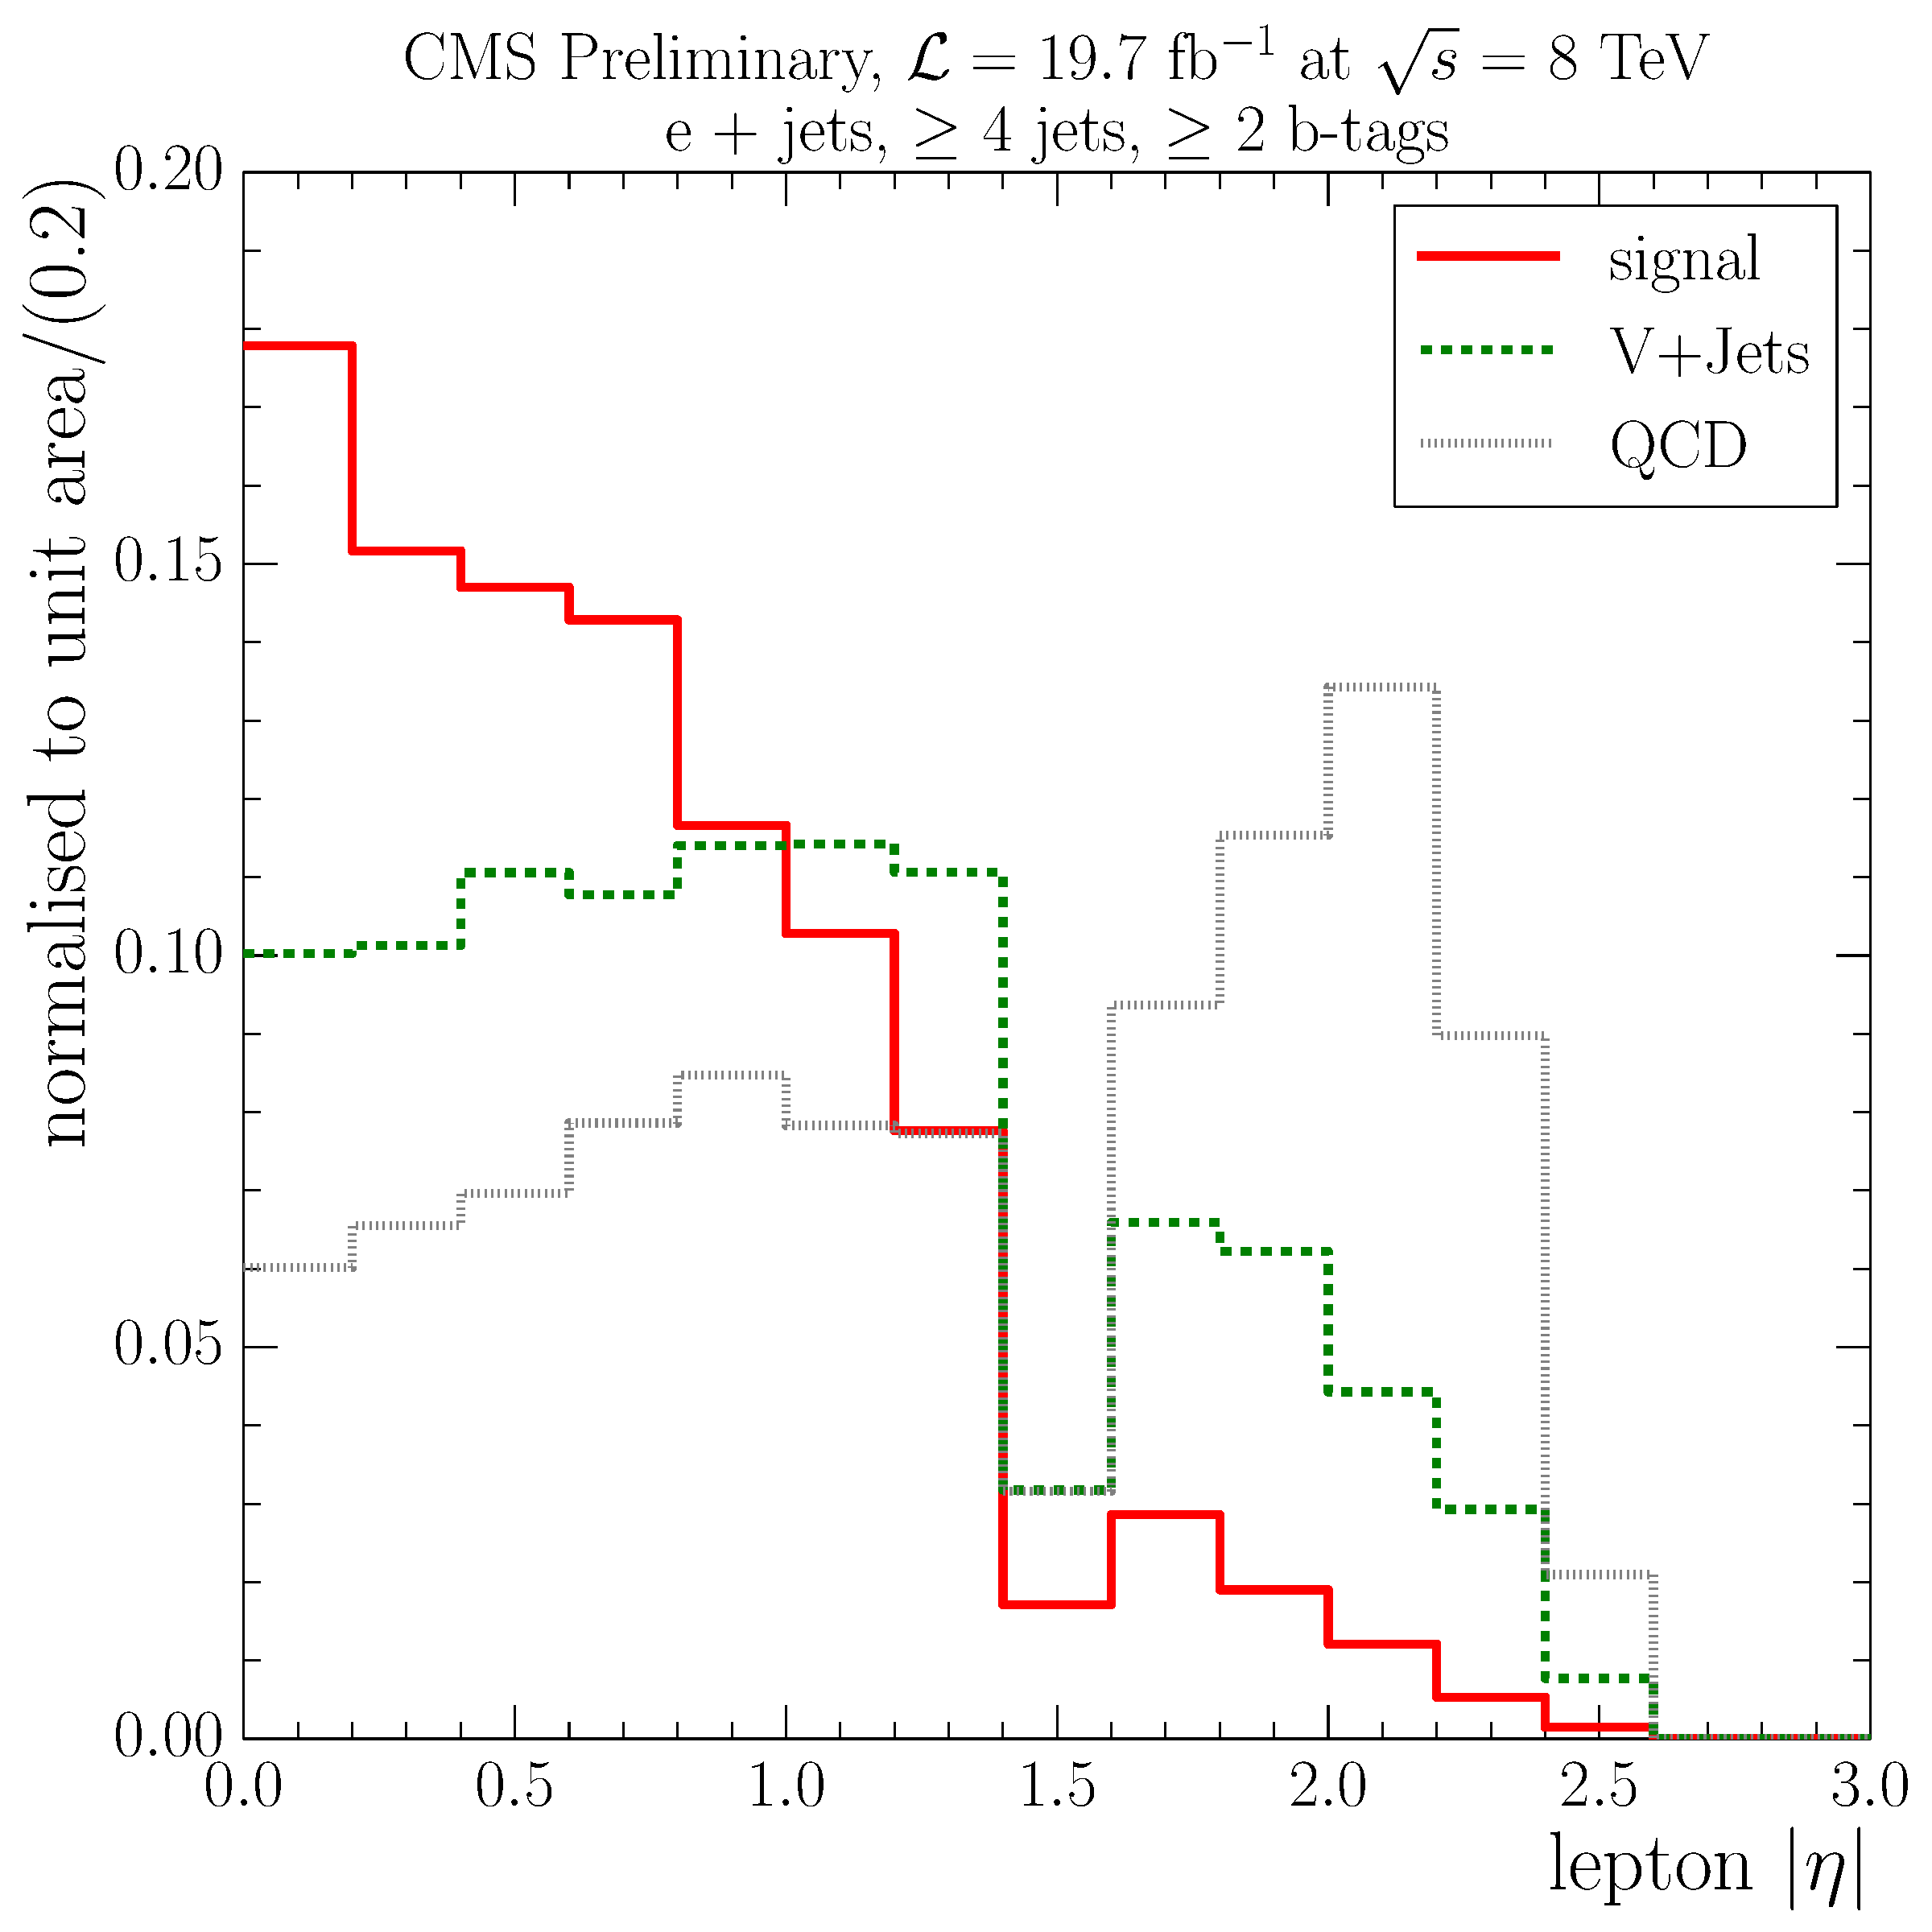
\includegraphics[width=0.3\textwidth]{measurement/HT/central/fit_templates/electron_templates_bin_600-inf}}
    \caption{Electron $\abs \eta$ templates for the fit in different bins of \HT,
    from top left to bottom right: \SIrange{0}{240}{\GeV}, \SIrange{240}{280}{\GeV},
    \SIrange{280}{330}{\GeV}, \SIrange{330}{380}{\GeV}, \SIrange{380}{450}{\GeV},
    \SIrange{450}{600}{\GeV} and $\geq \SI{600}{\GeV}$.}
    \label{fig:fit_tempaltes_HT_electron}
\end{figure}

\begin{figure}[!htbp]
	\centering
  	{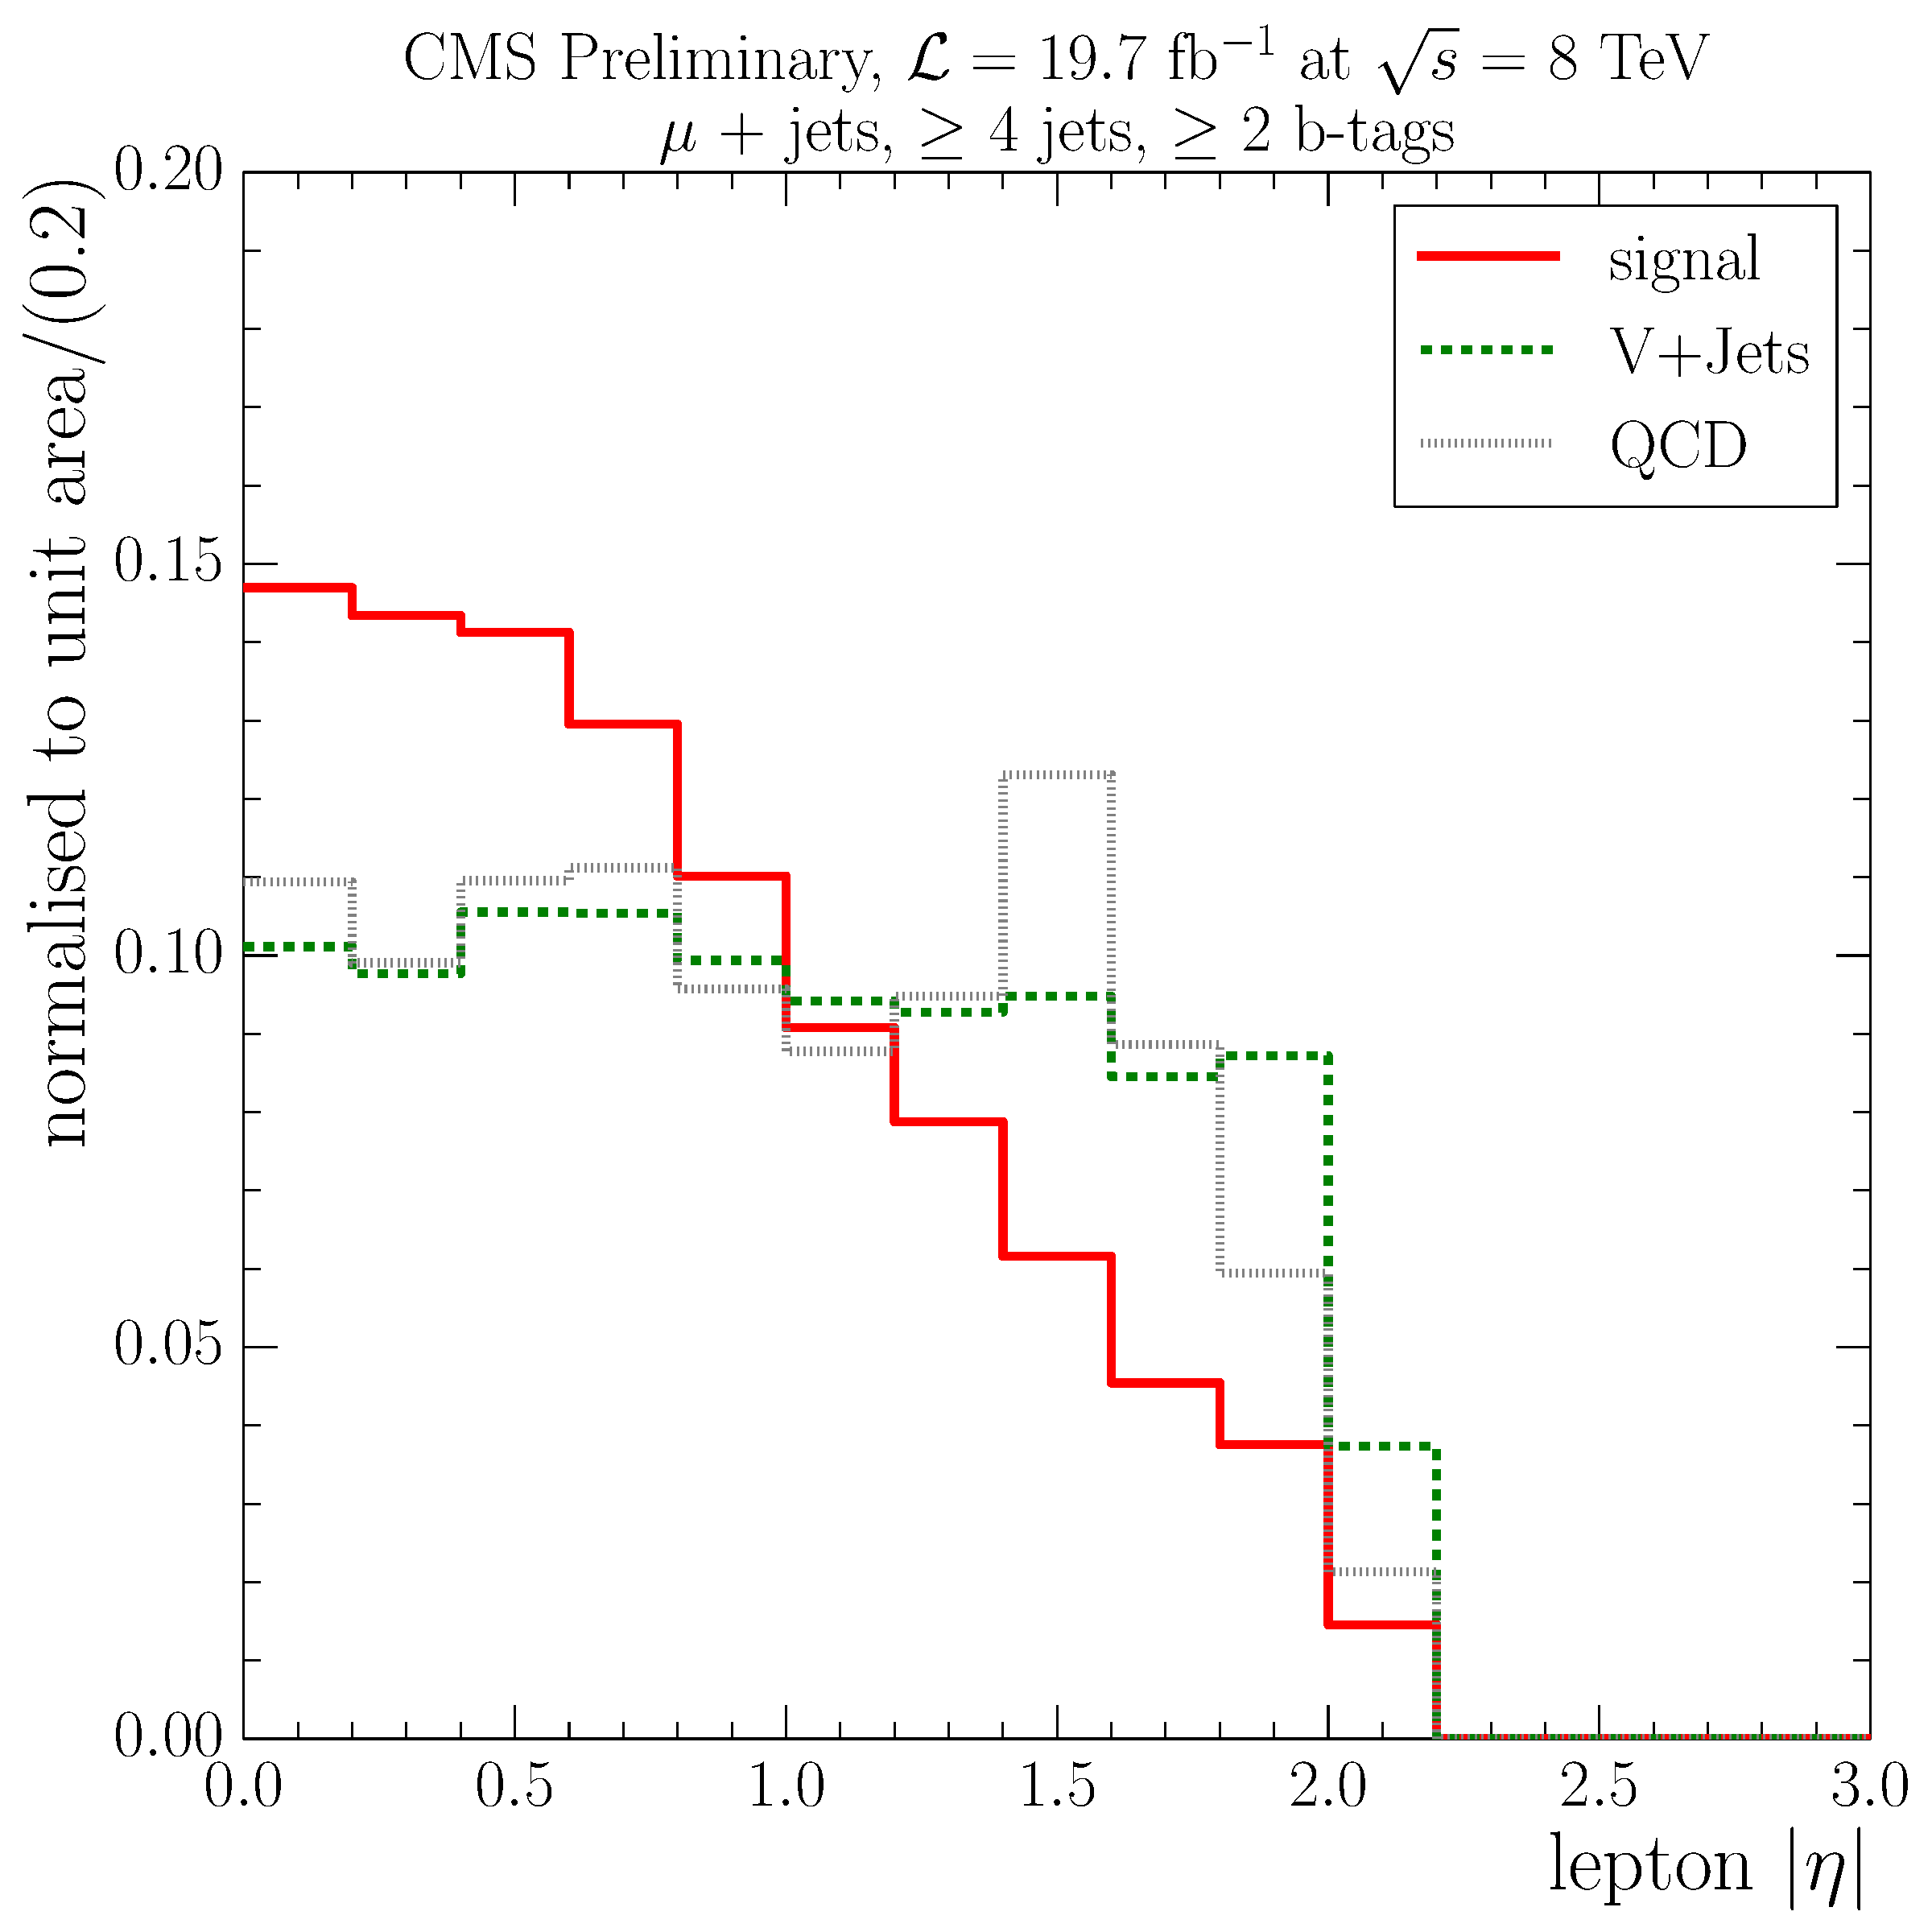
\includegraphics[width=0.3\textwidth]{measurement/HT/central/fit_templates/muon_templates_bin_0-240}}
  	{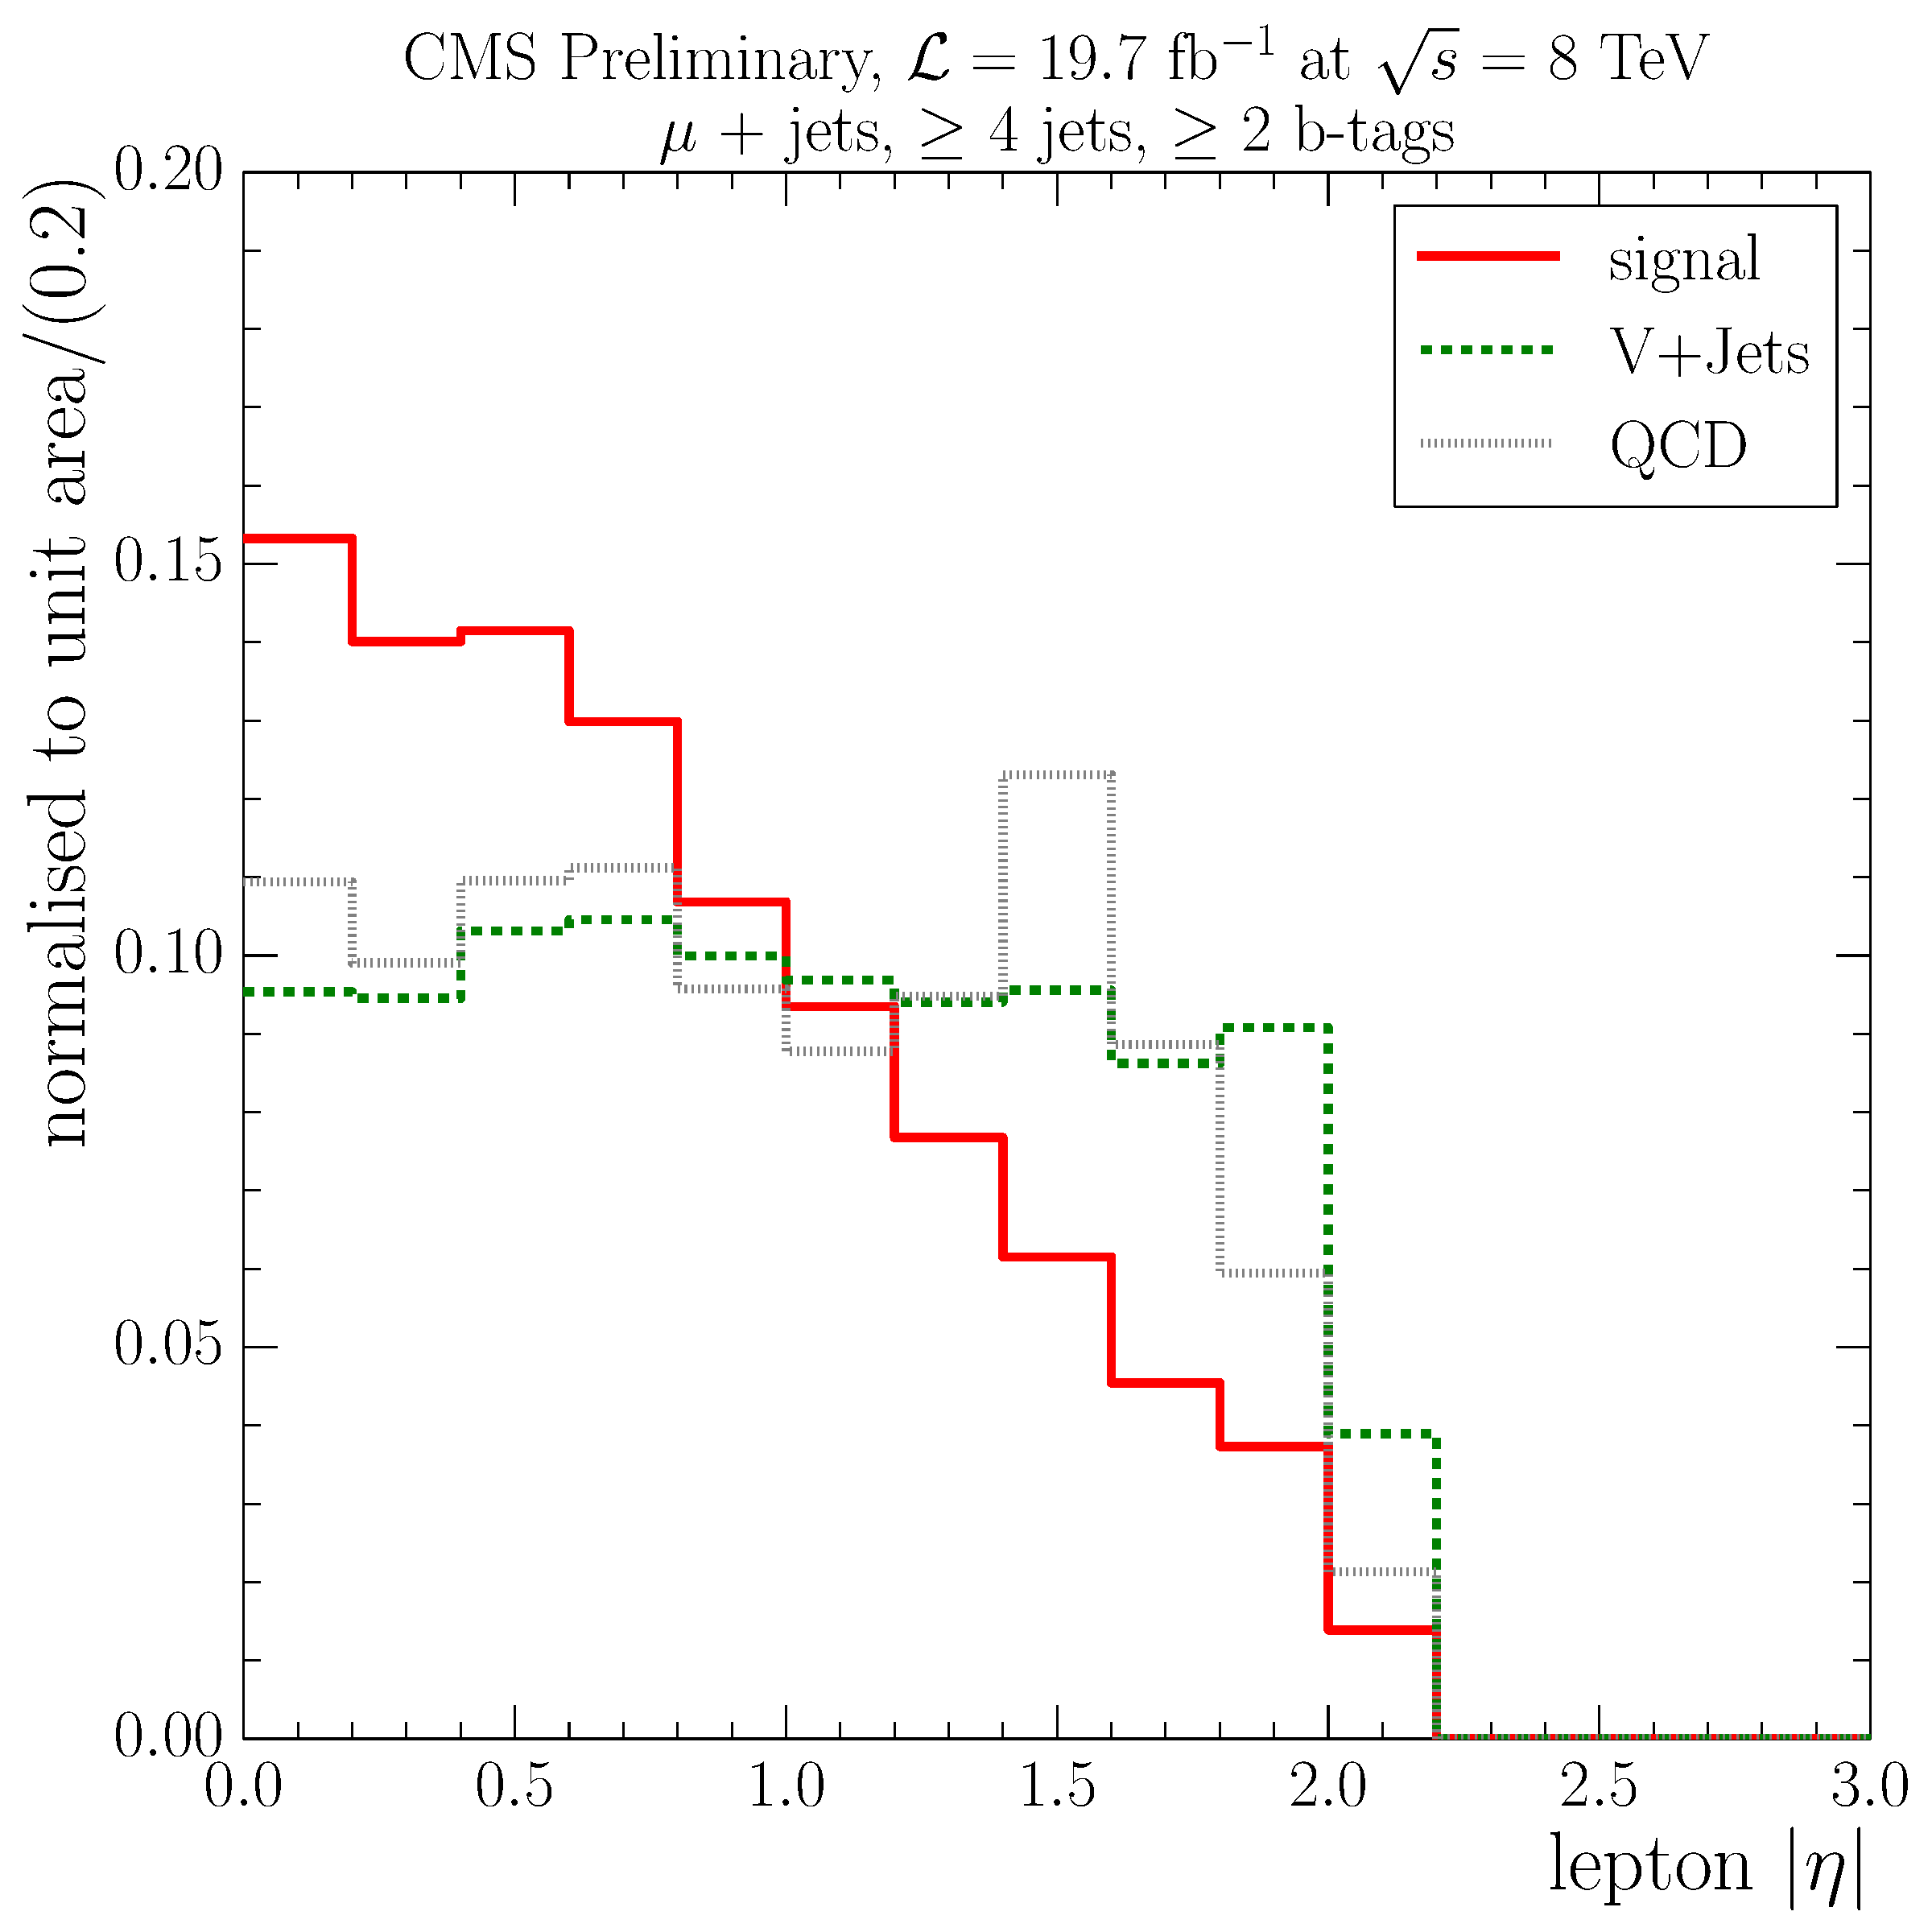
\includegraphics[width=0.3\textwidth]{measurement/HT/central/fit_templates/muon_templates_bin_240-280}}
  	{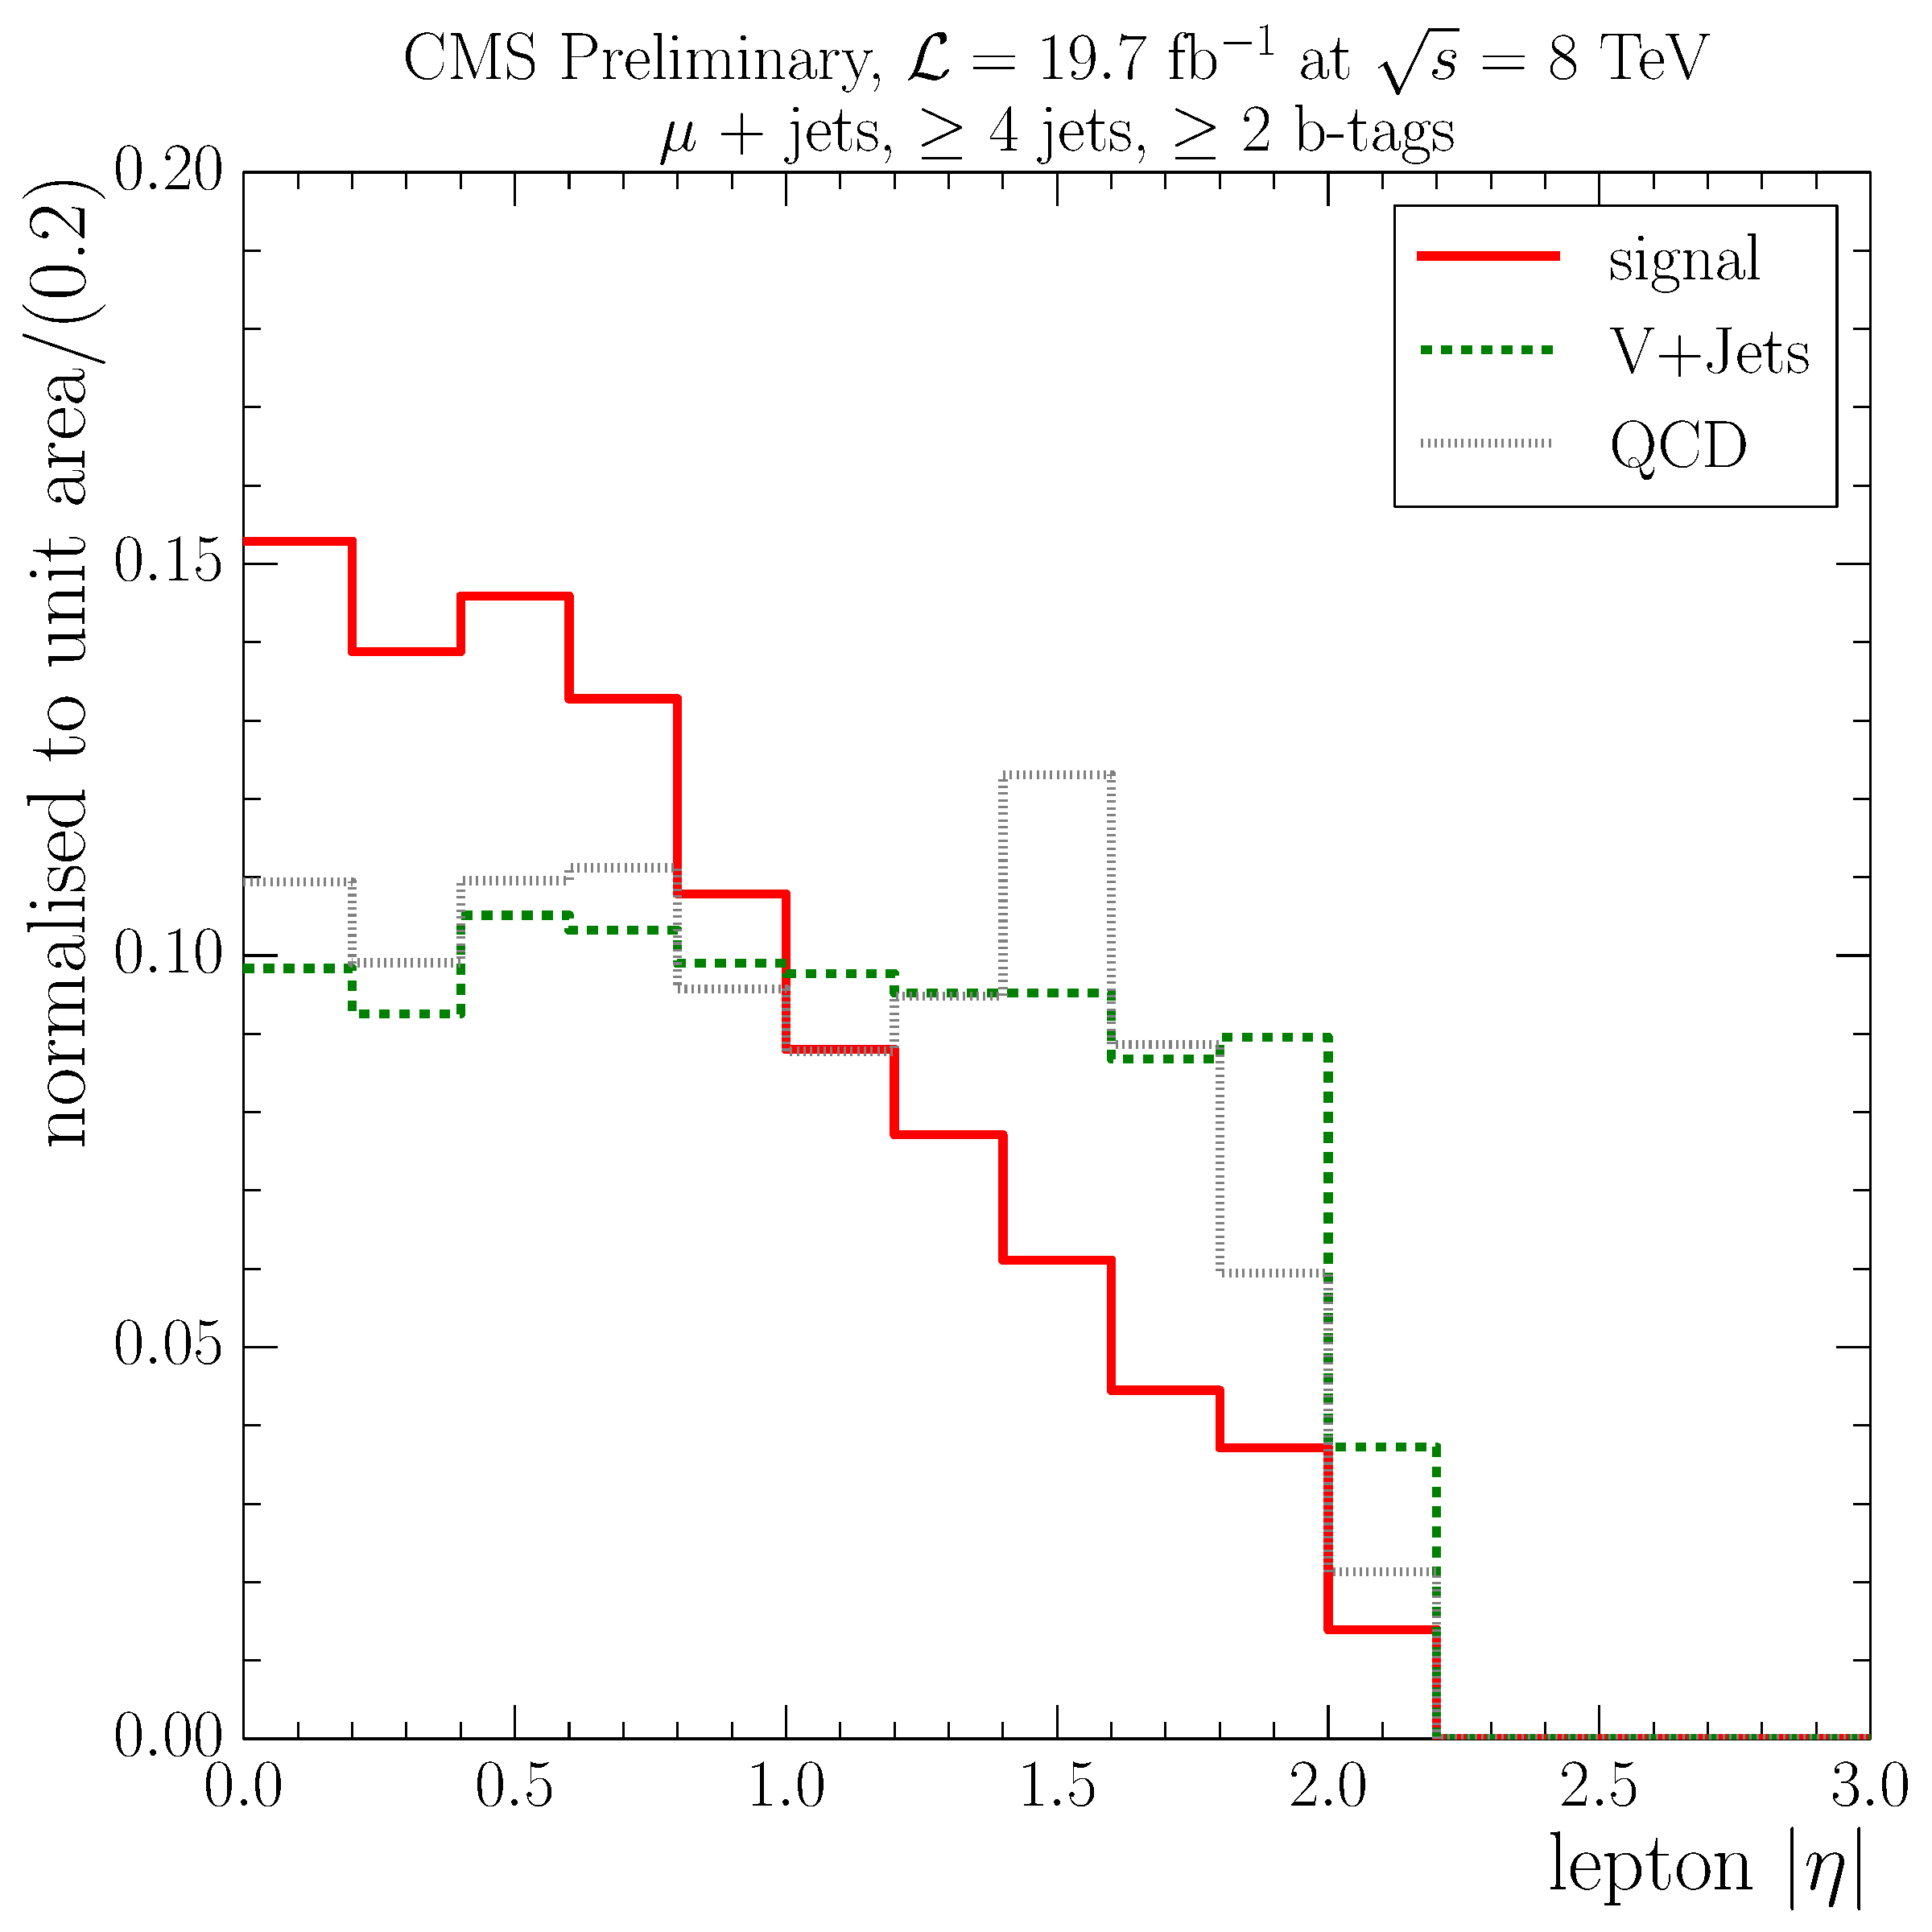
\includegraphics[width=0.3\textwidth]{measurement/HT/central/fit_templates/muon_templates_bin_280-330}}\\
  	{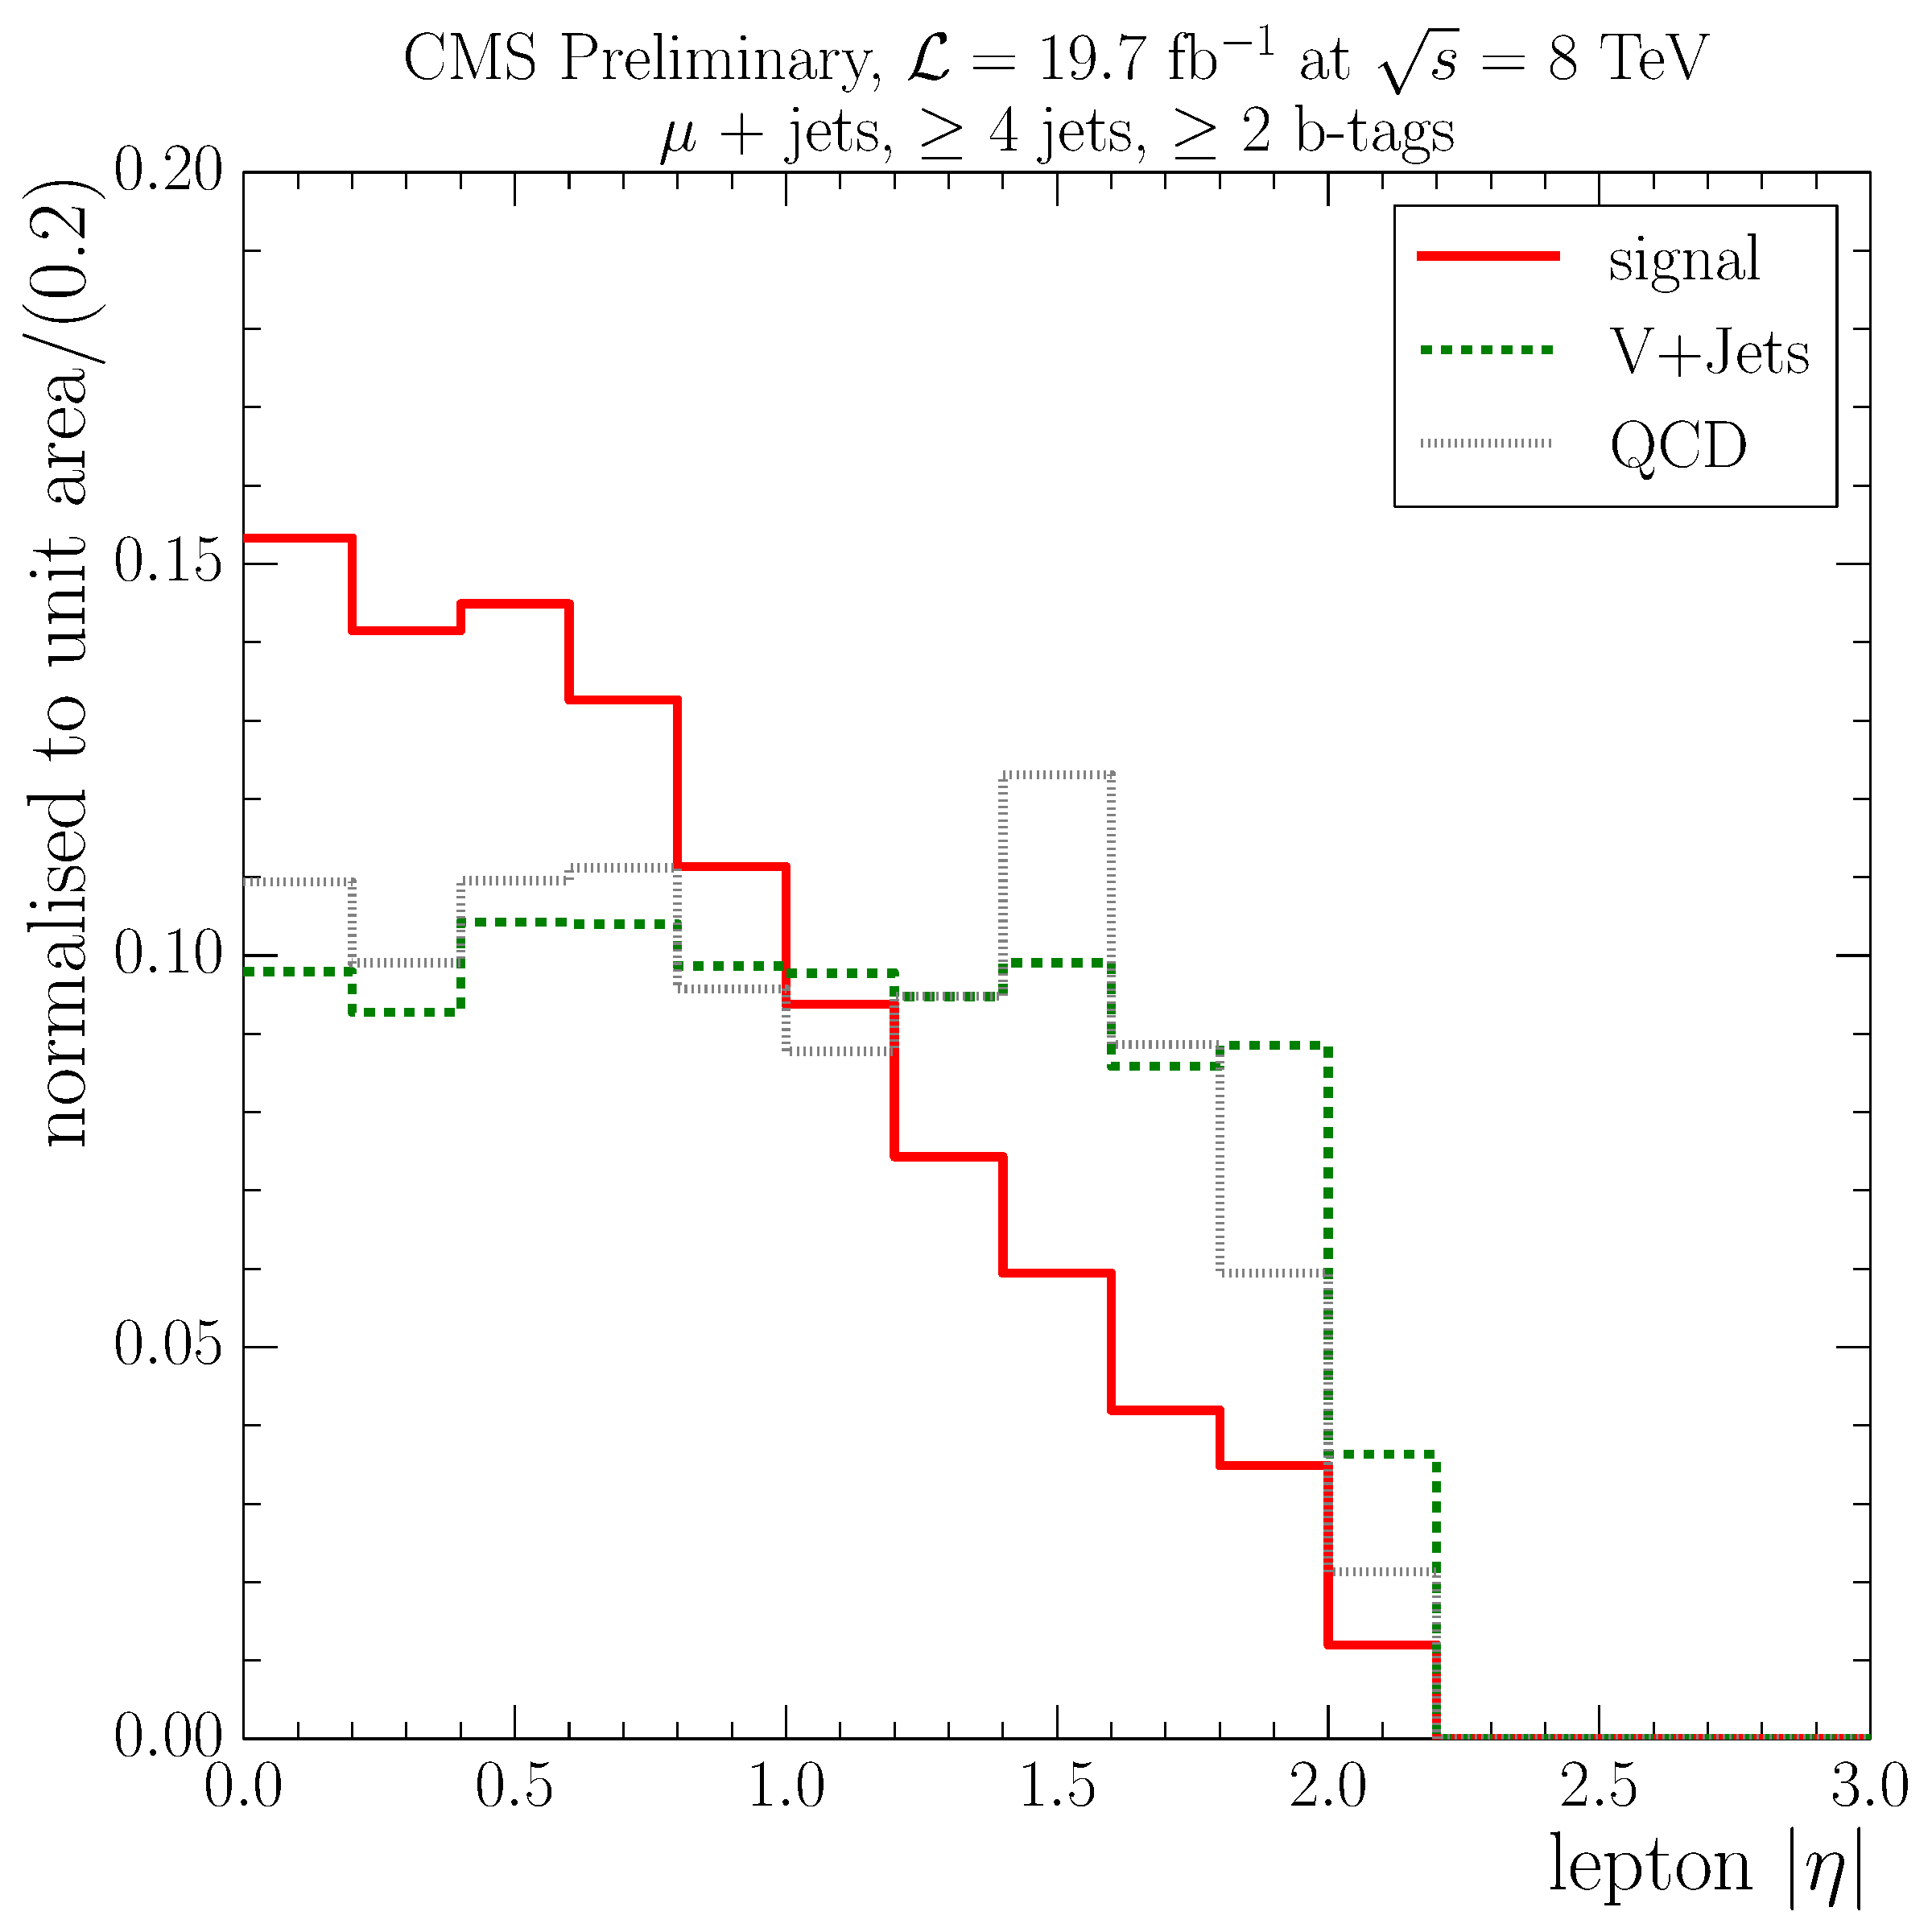
\includegraphics[width=0.3\textwidth]{measurement/HT/central/fit_templates/muon_templates_bin_330-380}}
  	{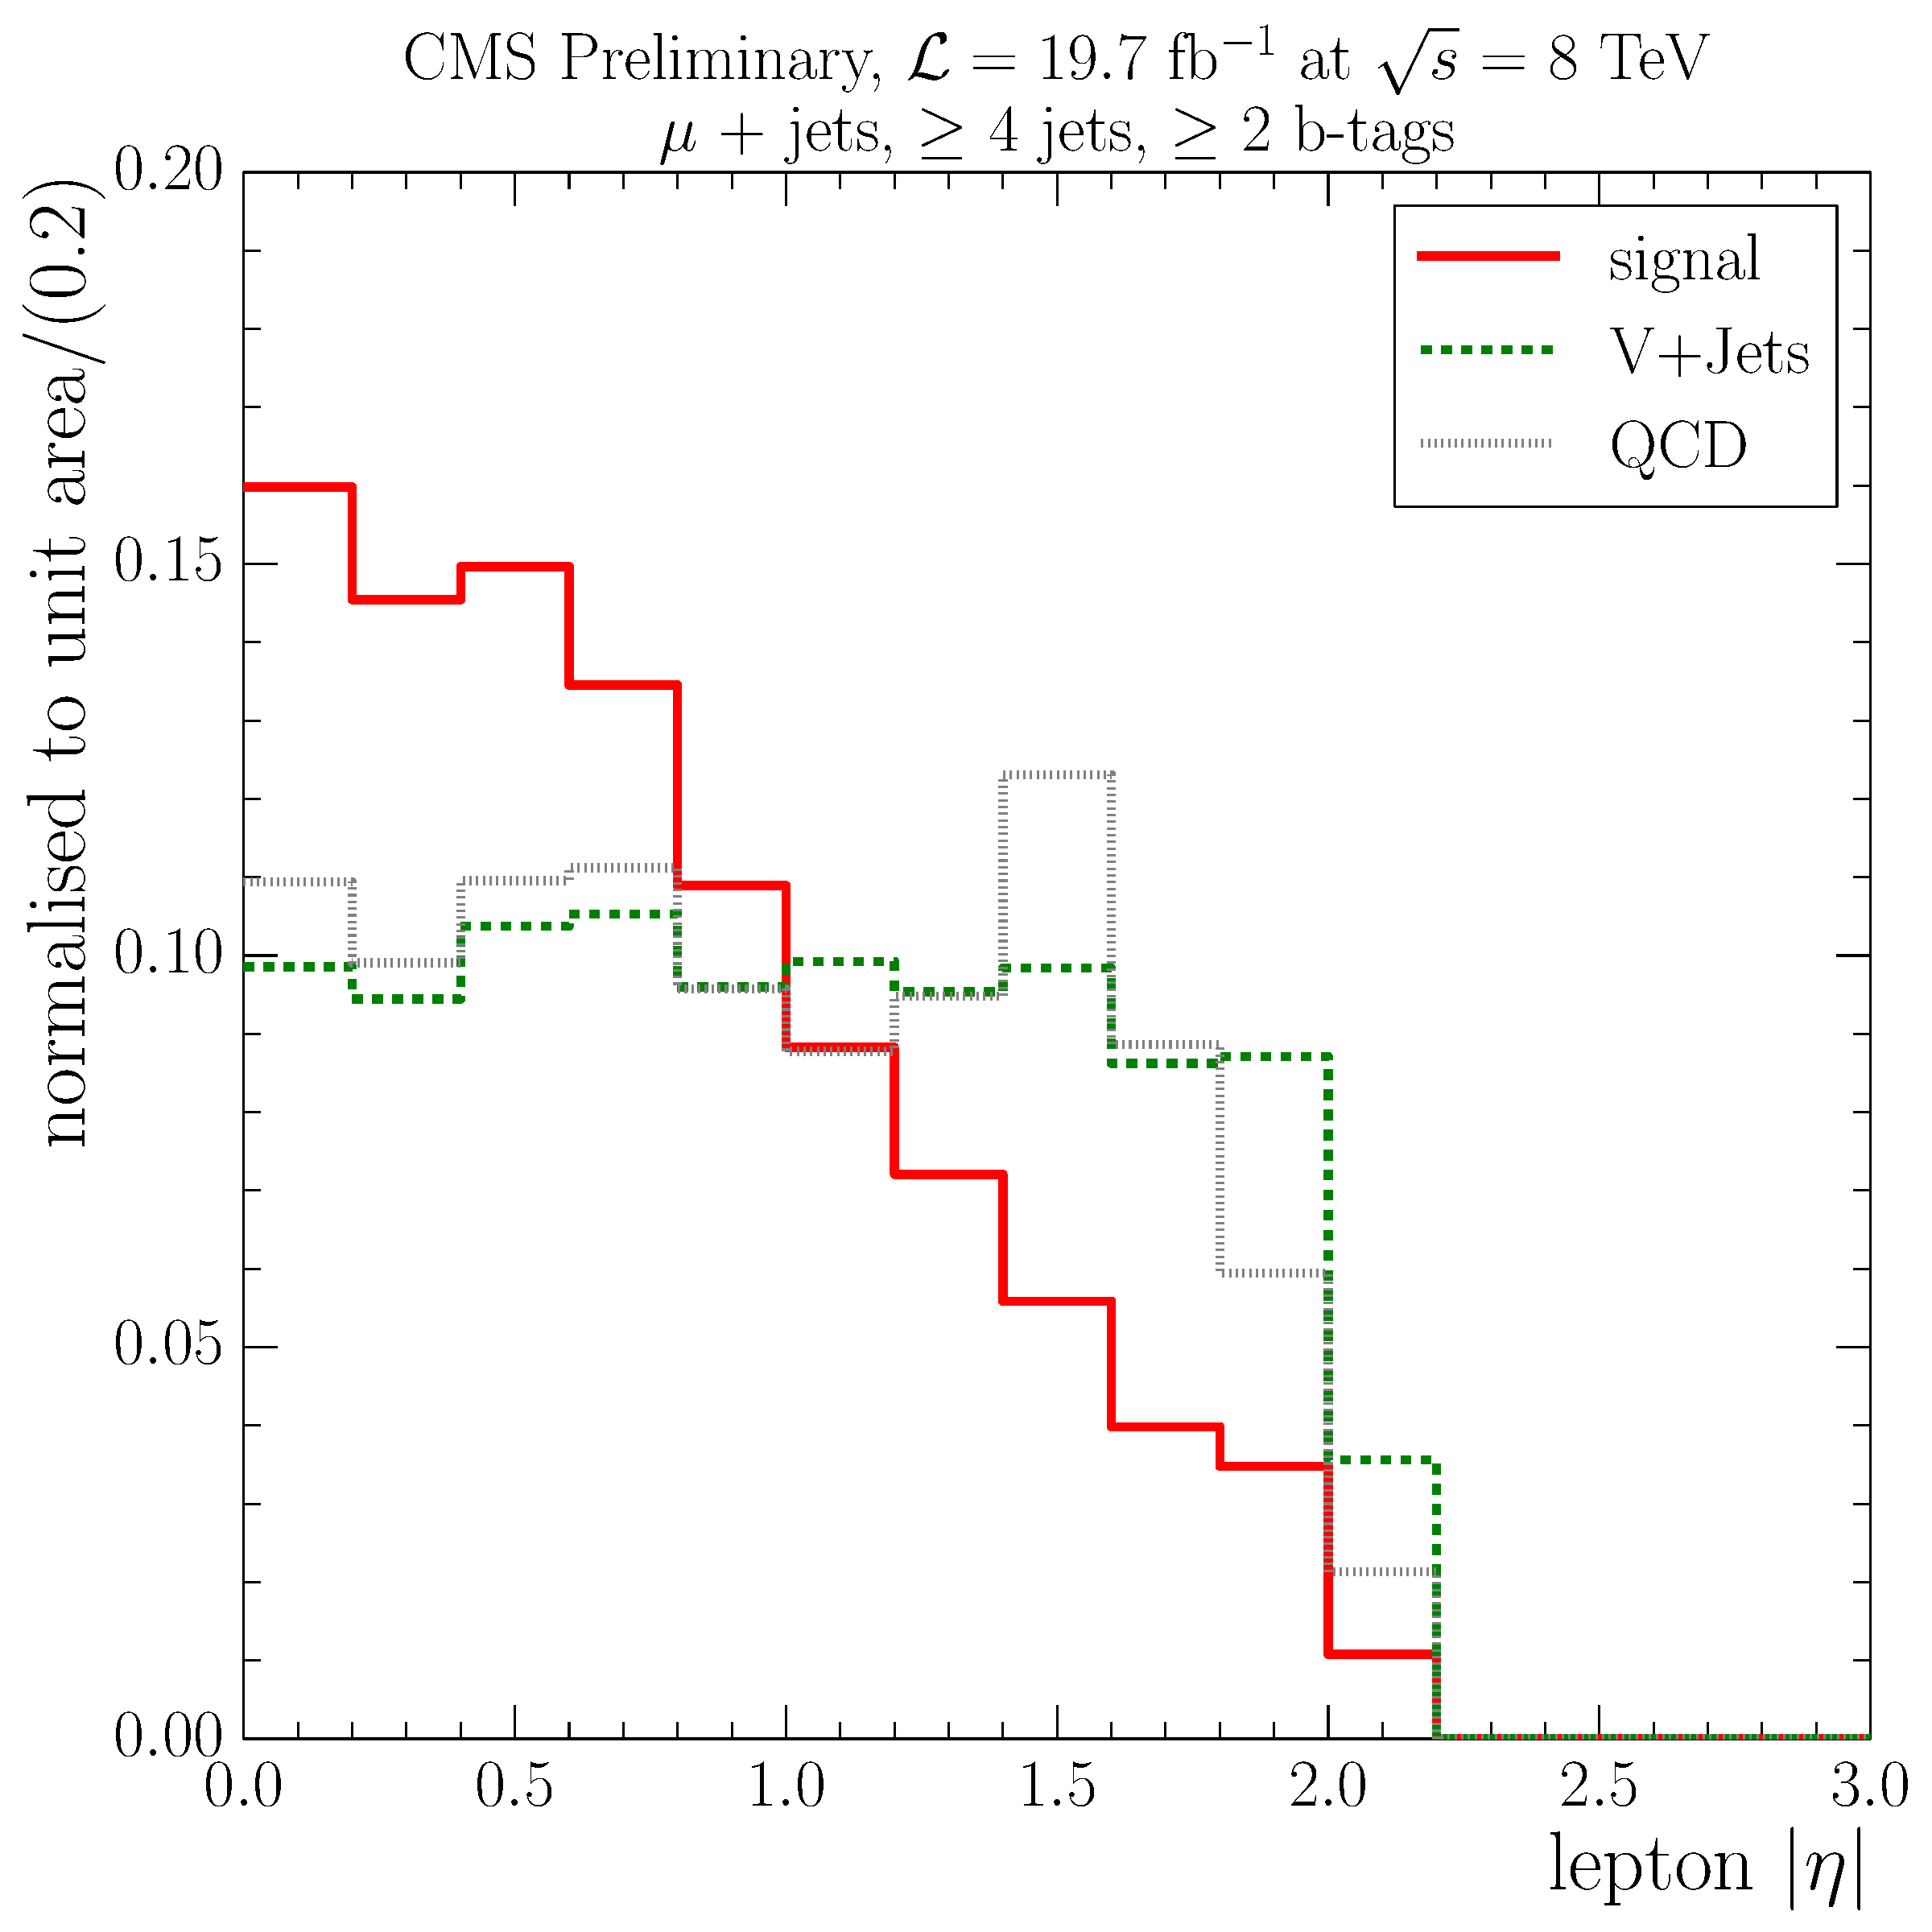
\includegraphics[width=0.3\textwidth]{measurement/HT/central/fit_templates/muon_templates_bin_380-450}}
  	{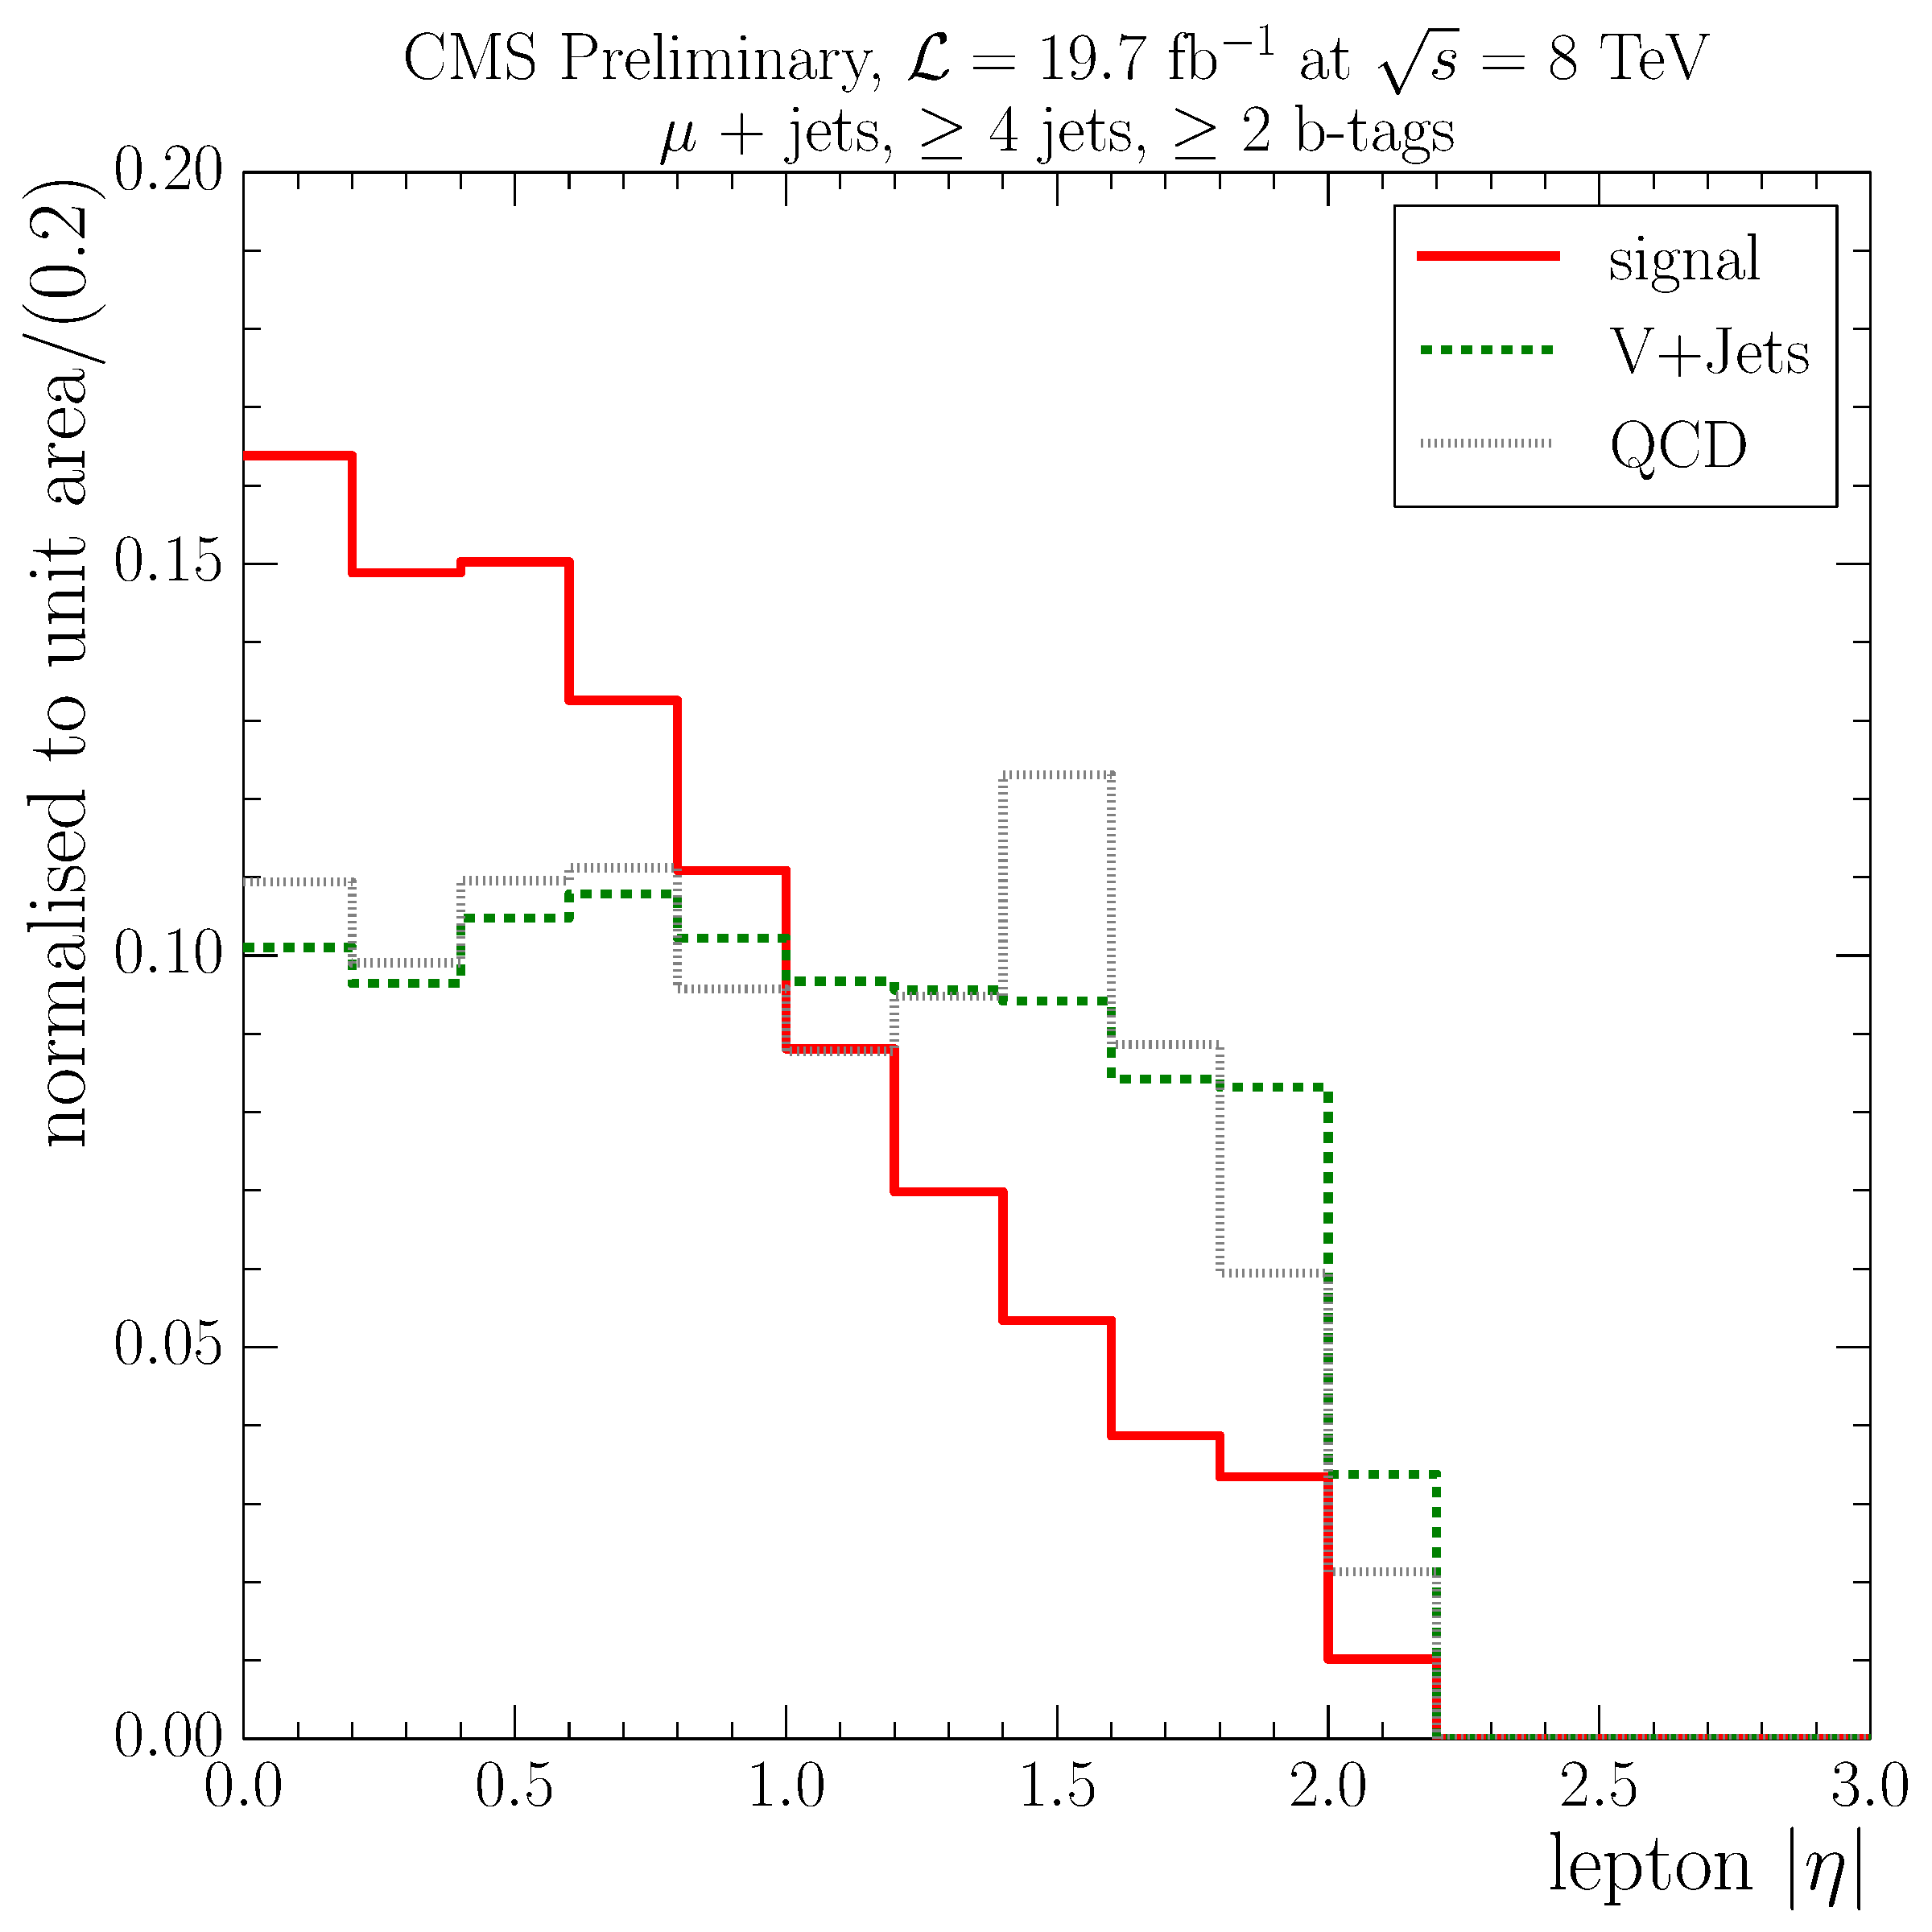
\includegraphics[width=0.3\textwidth]{measurement/HT/central/fit_templates/muon_templates_bin_450-600}}\\
  	{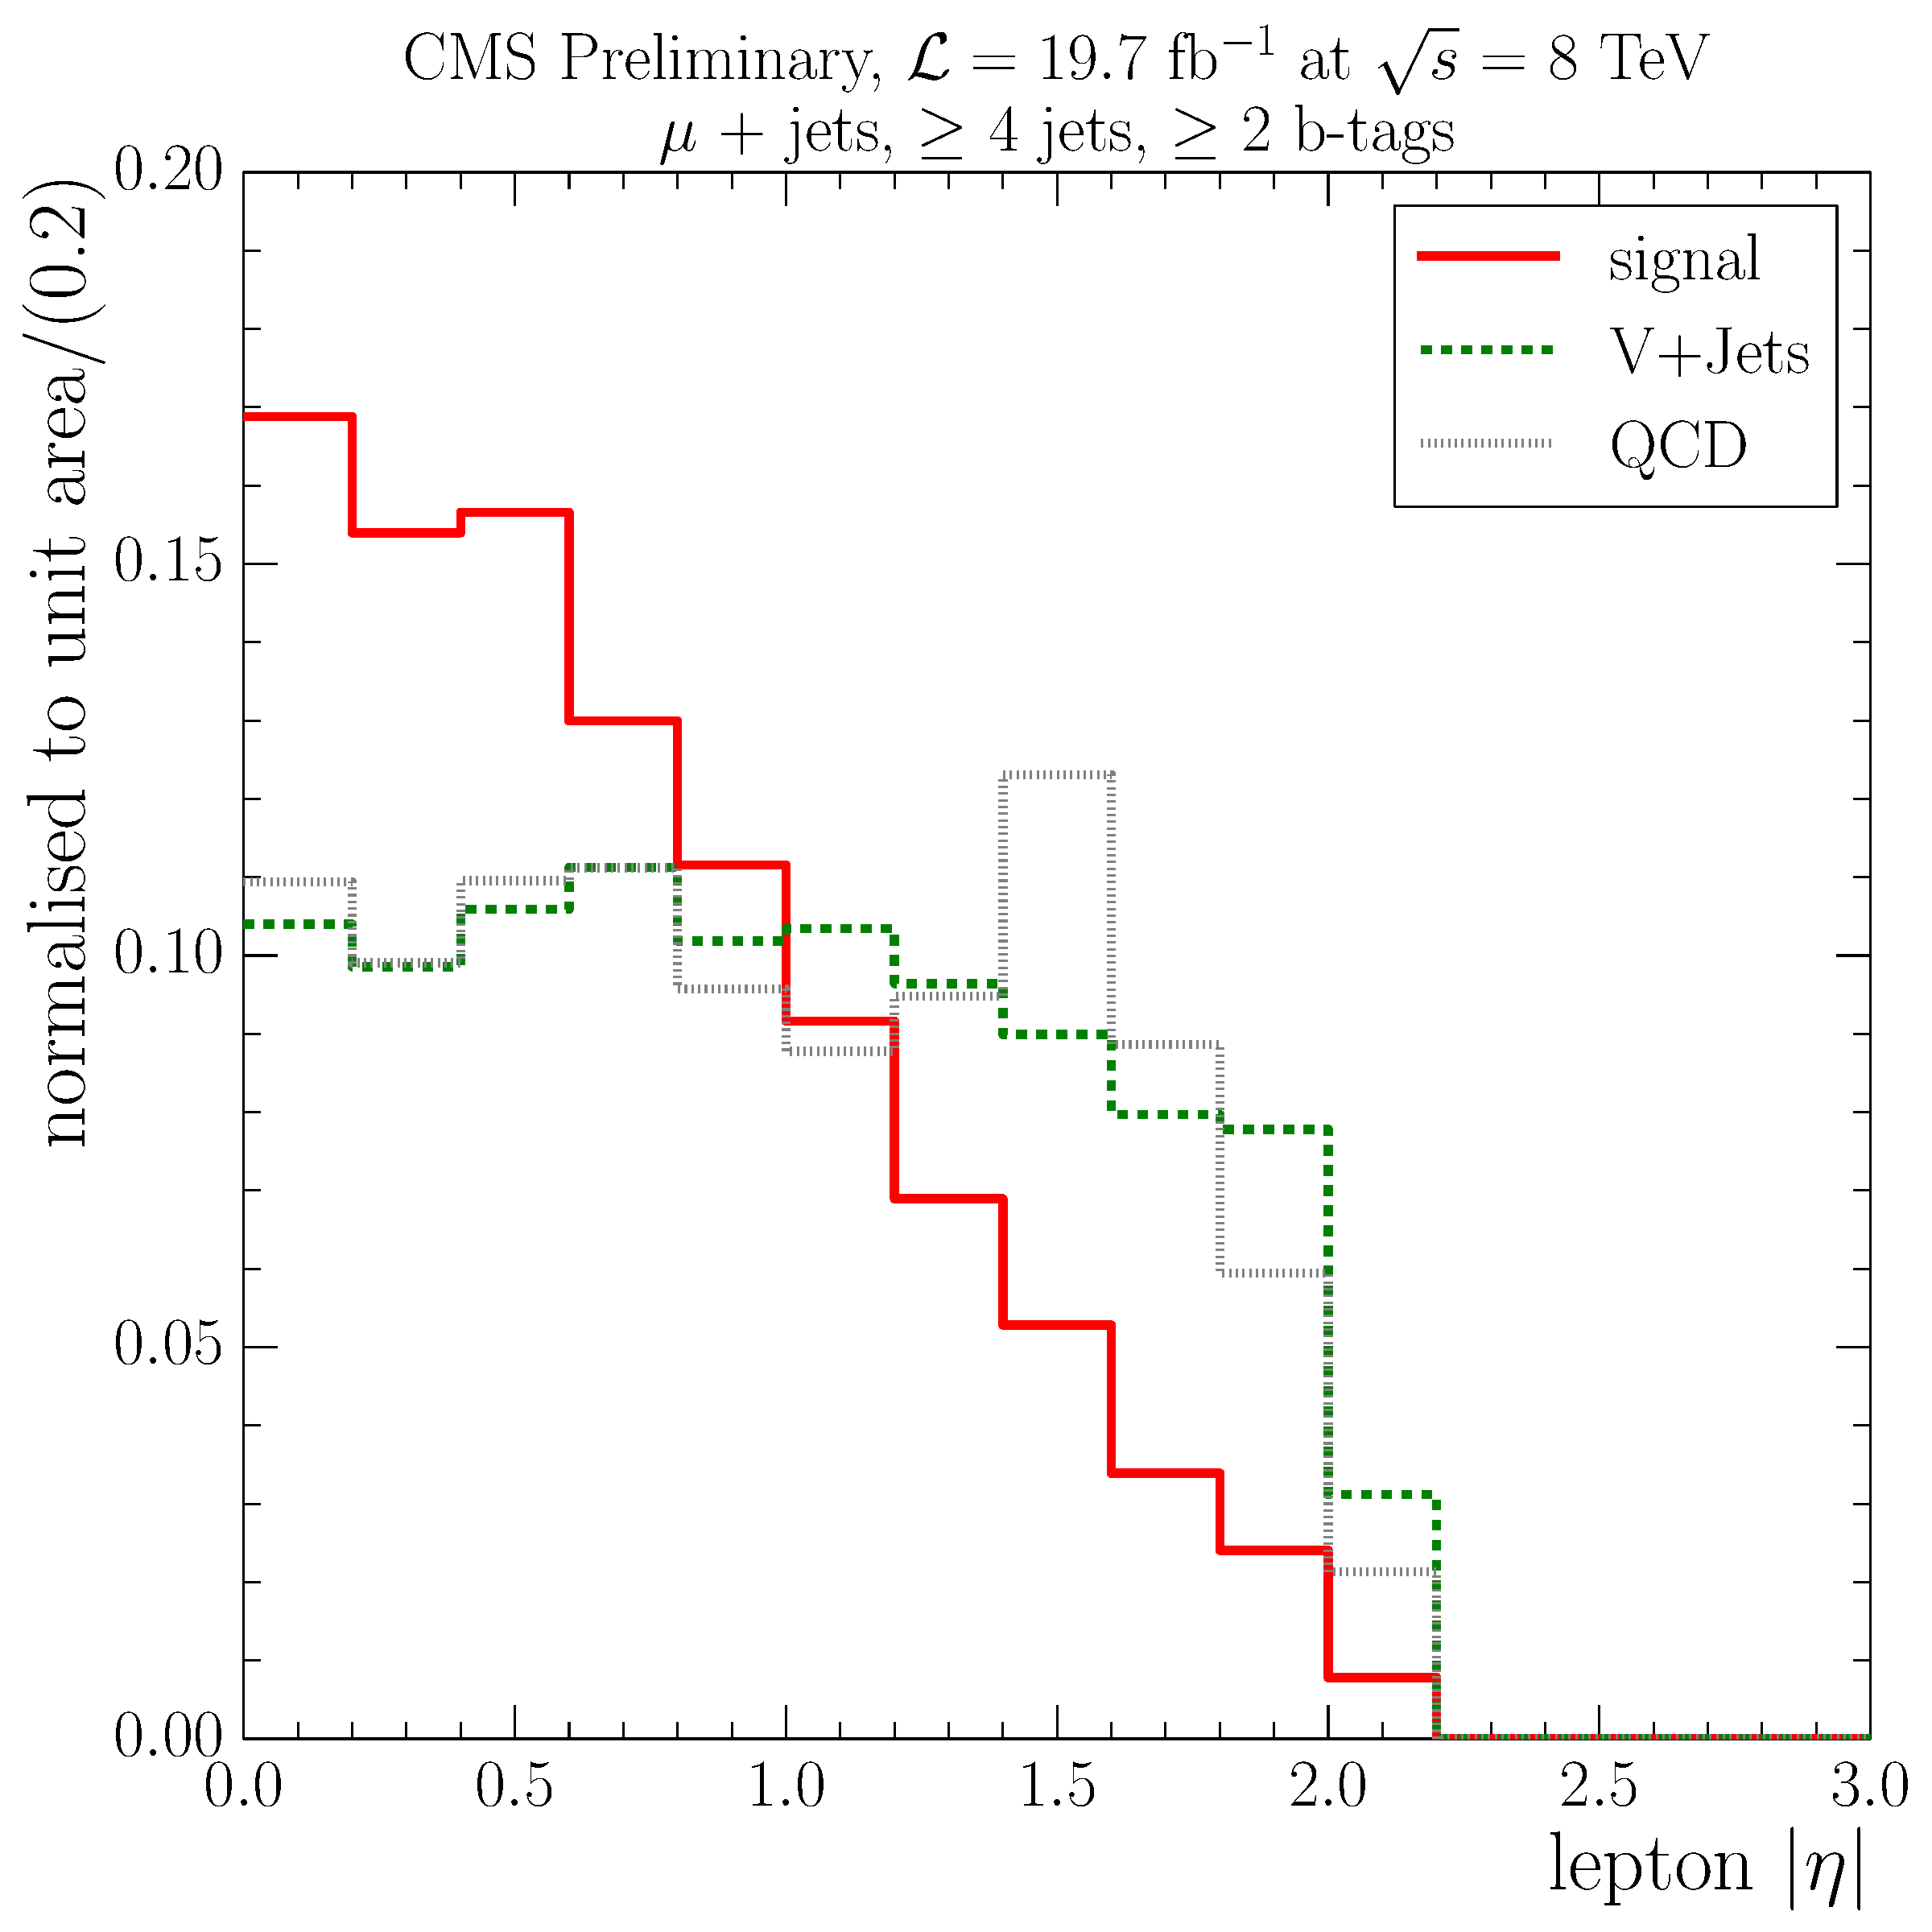
\includegraphics[width=0.3\textwidth]{measurement/HT/central/fit_templates/muon_templates_bin_600-inf}}
    \caption{Electron $\abs \eta$ templates for the fit in different bins of \HT,
    from top left to bottom right: \SIrange{0}{240}{\GeV}, \SIrange{240}{280}{\GeV},
    \SIrange{280}{330}{\GeV}, \SIrange{330}{380}{\GeV}, \SIrange{380}{450}{\GeV},
    \SIrange{450}{600}{\GeV} and $\geq \SI{600}{\GeV}$.}
    \label{fig:fit_templates_HT_muon}
\end{figure}

\newpage
\section*{\ST variable}

\begin{figure}[!htbp]
  \centering
    {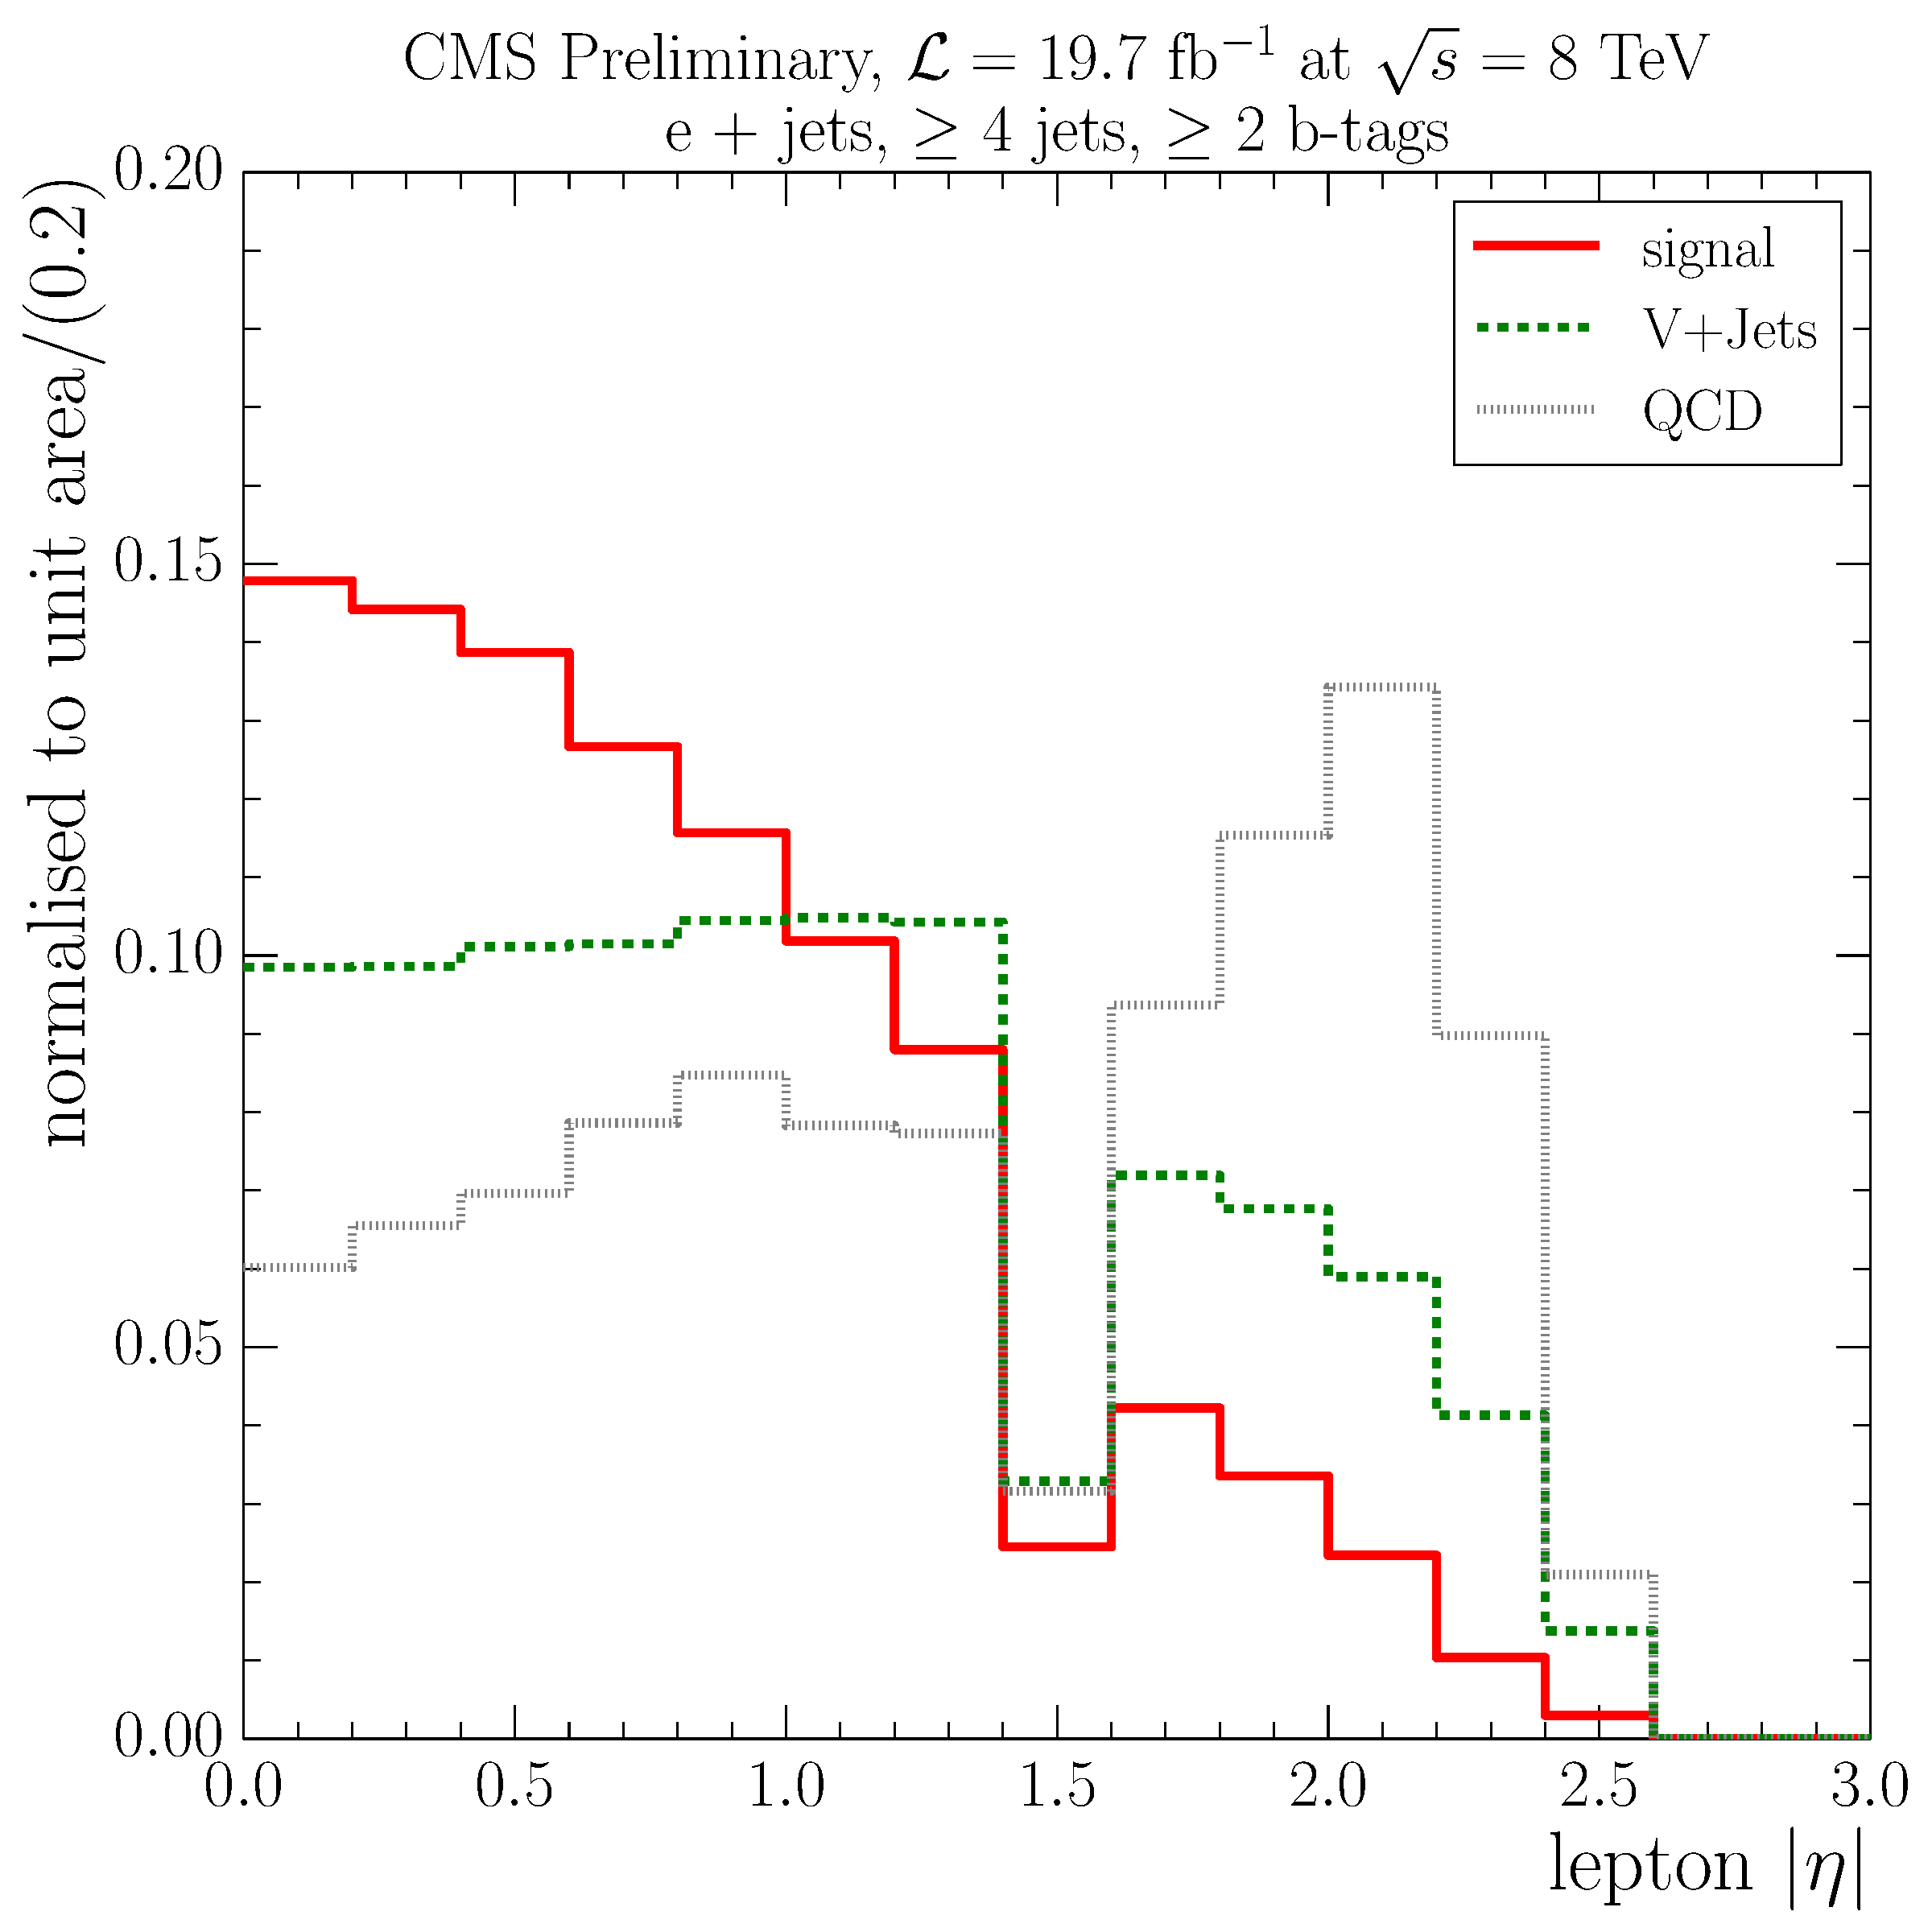
\includegraphics[width=0.3\textwidth]{measurement/ST/central/fit_templates/electron_templates_bin_0-350}}
    {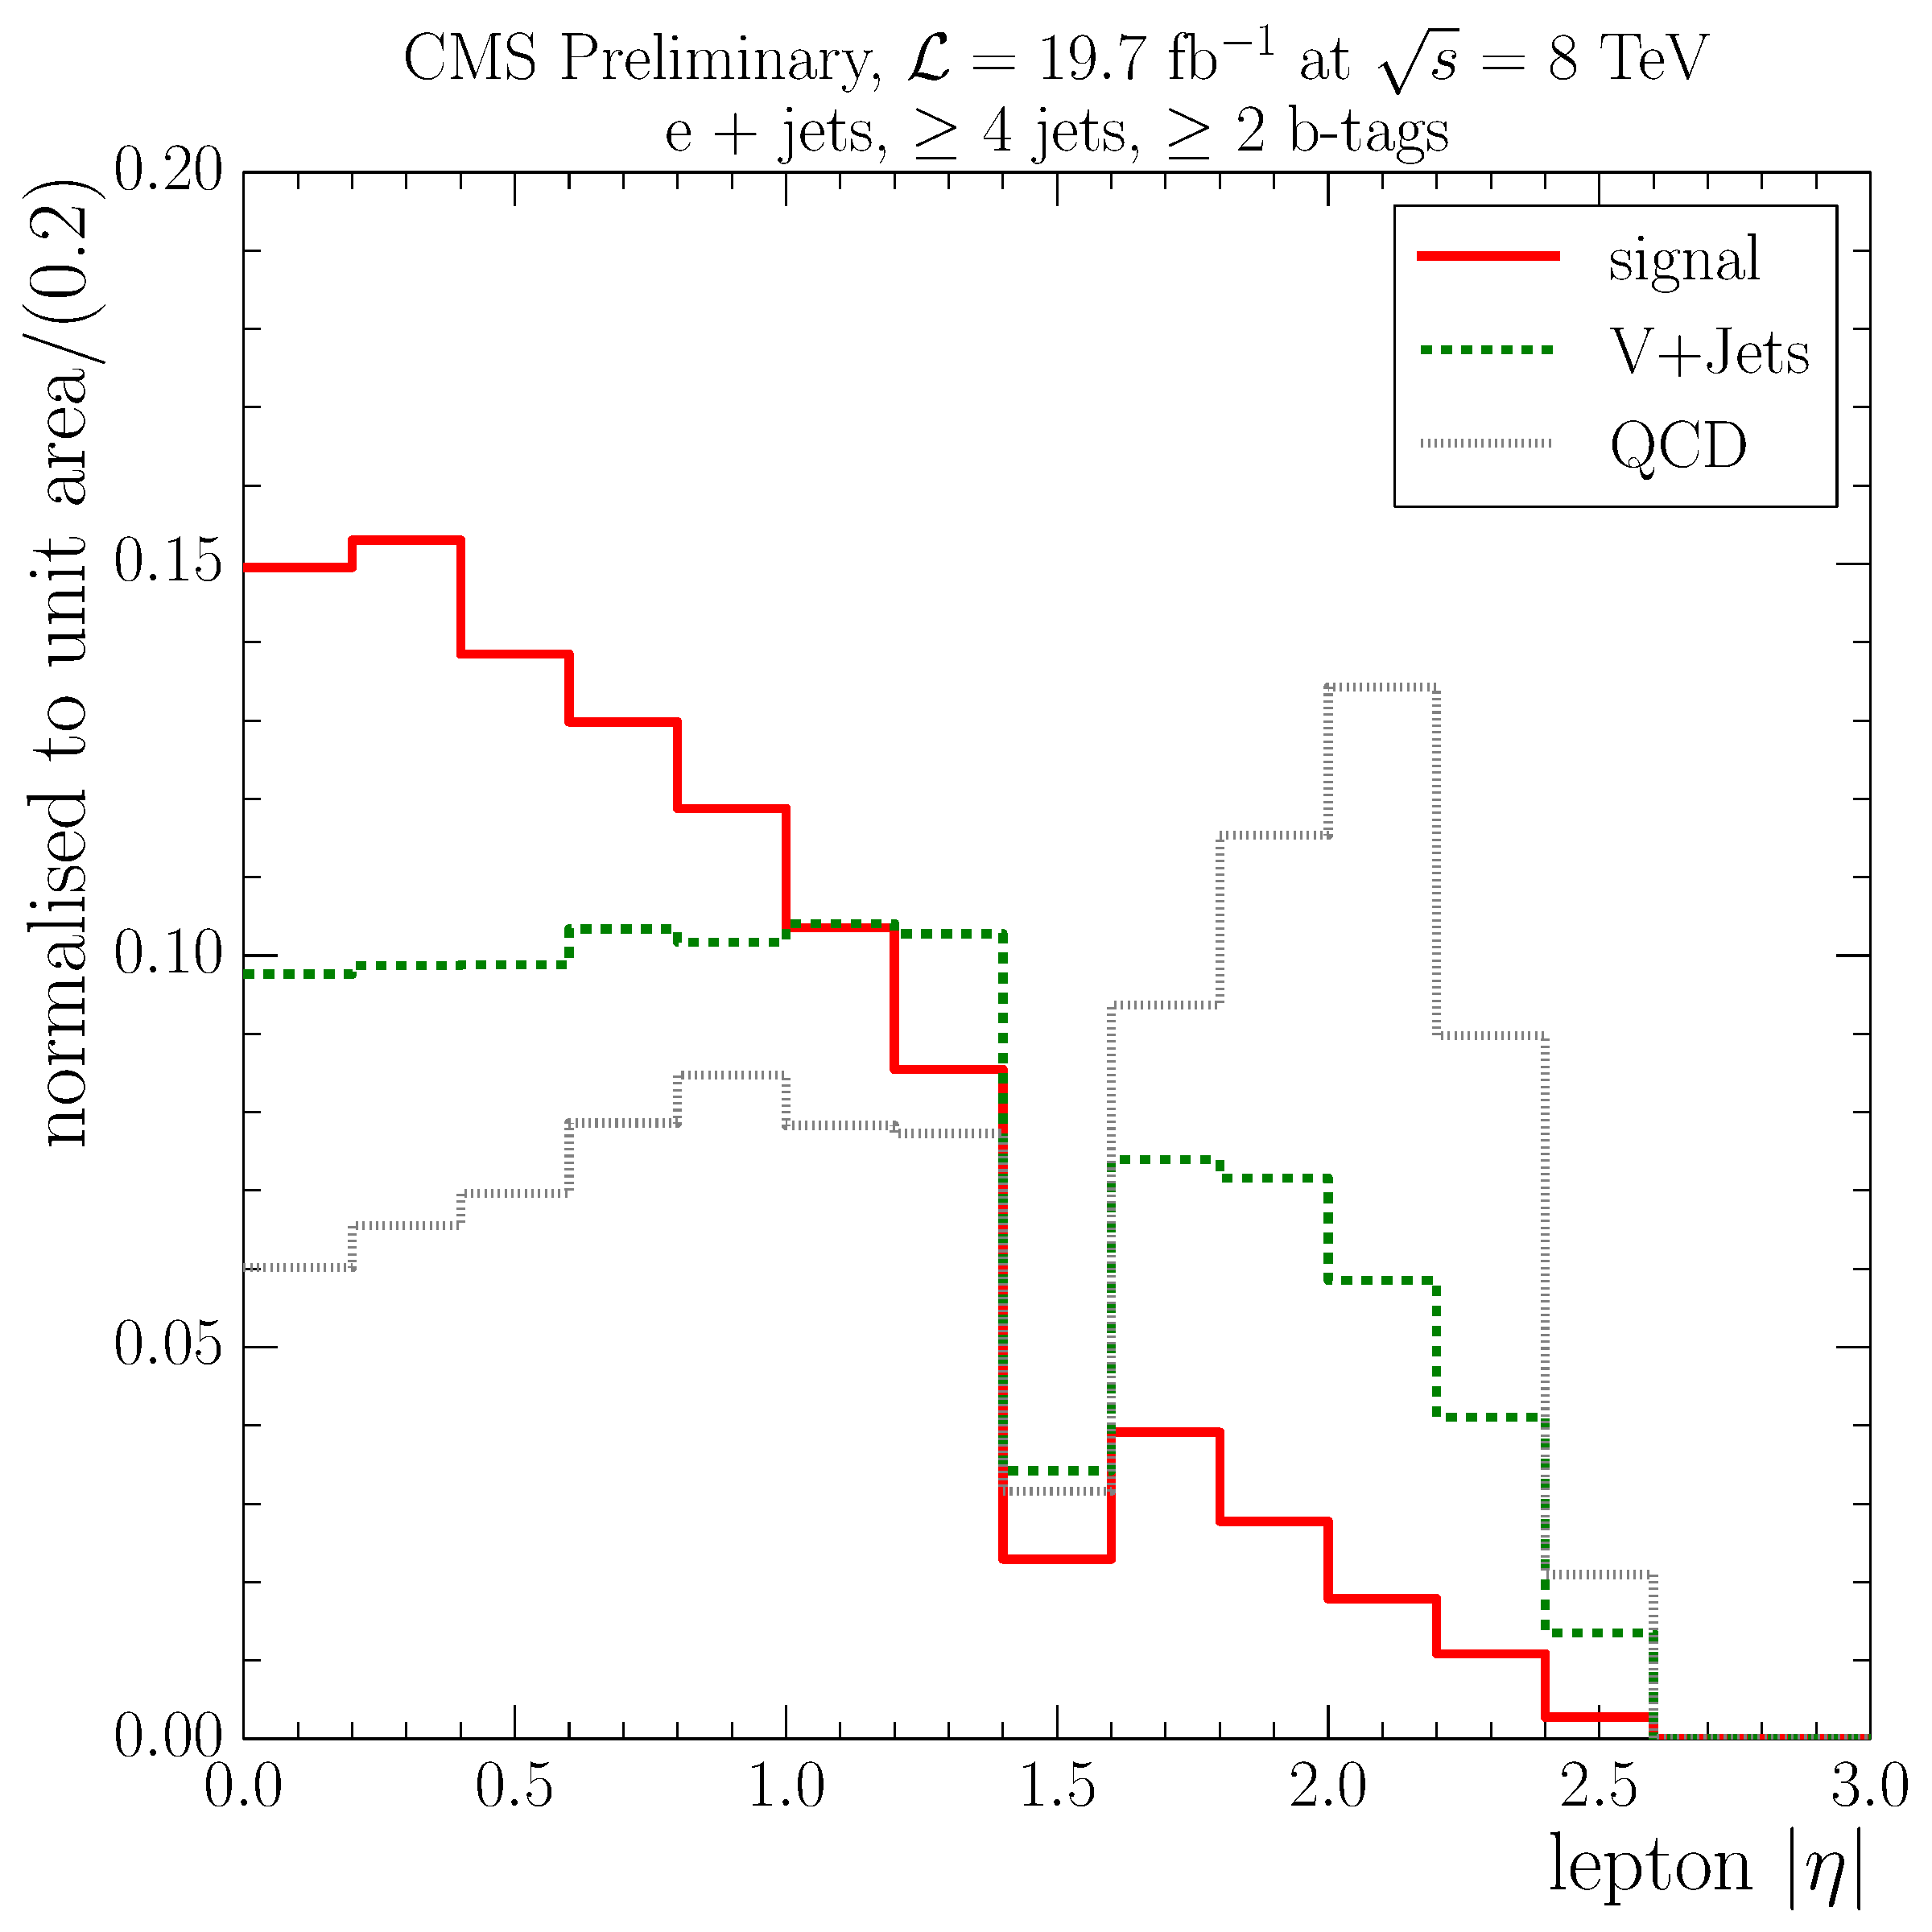
\includegraphics[width=0.3\textwidth]{measurement/ST/central/fit_templates/electron_templates_bin_350-400}}
    {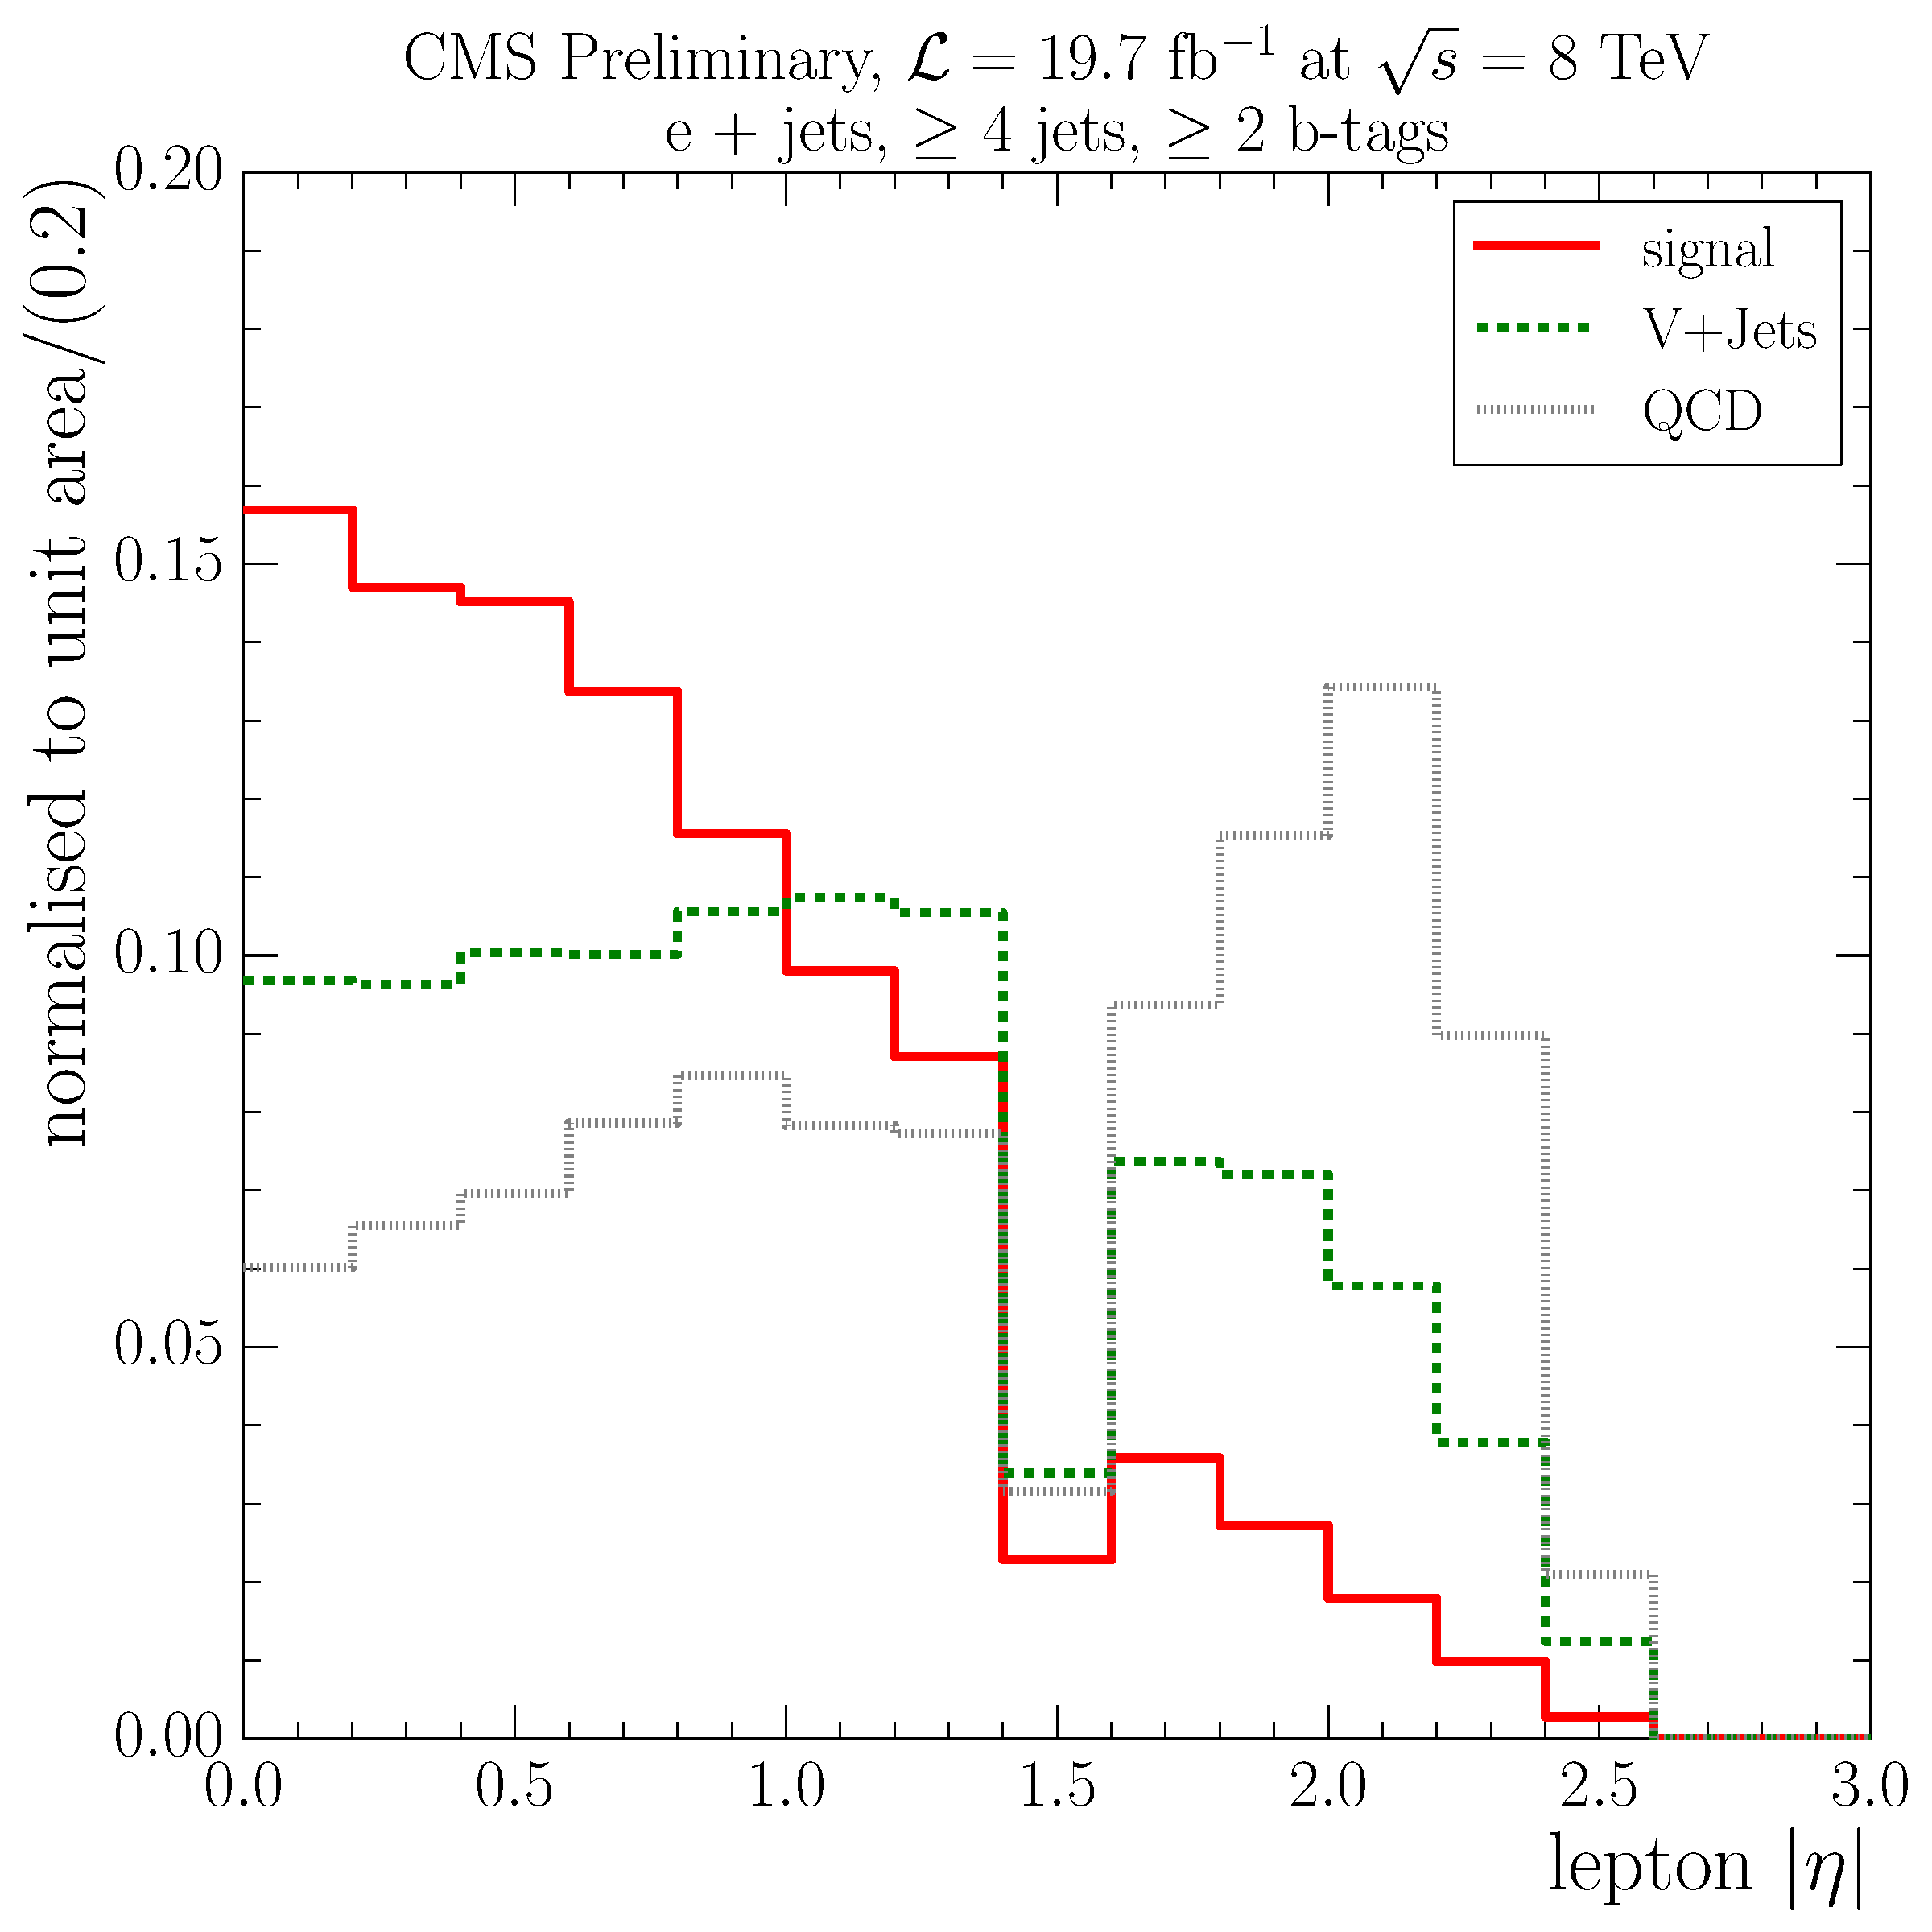
\includegraphics[width=0.3\textwidth]{measurement/ST/central/fit_templates/electron_templates_bin_400-450}}\\
    {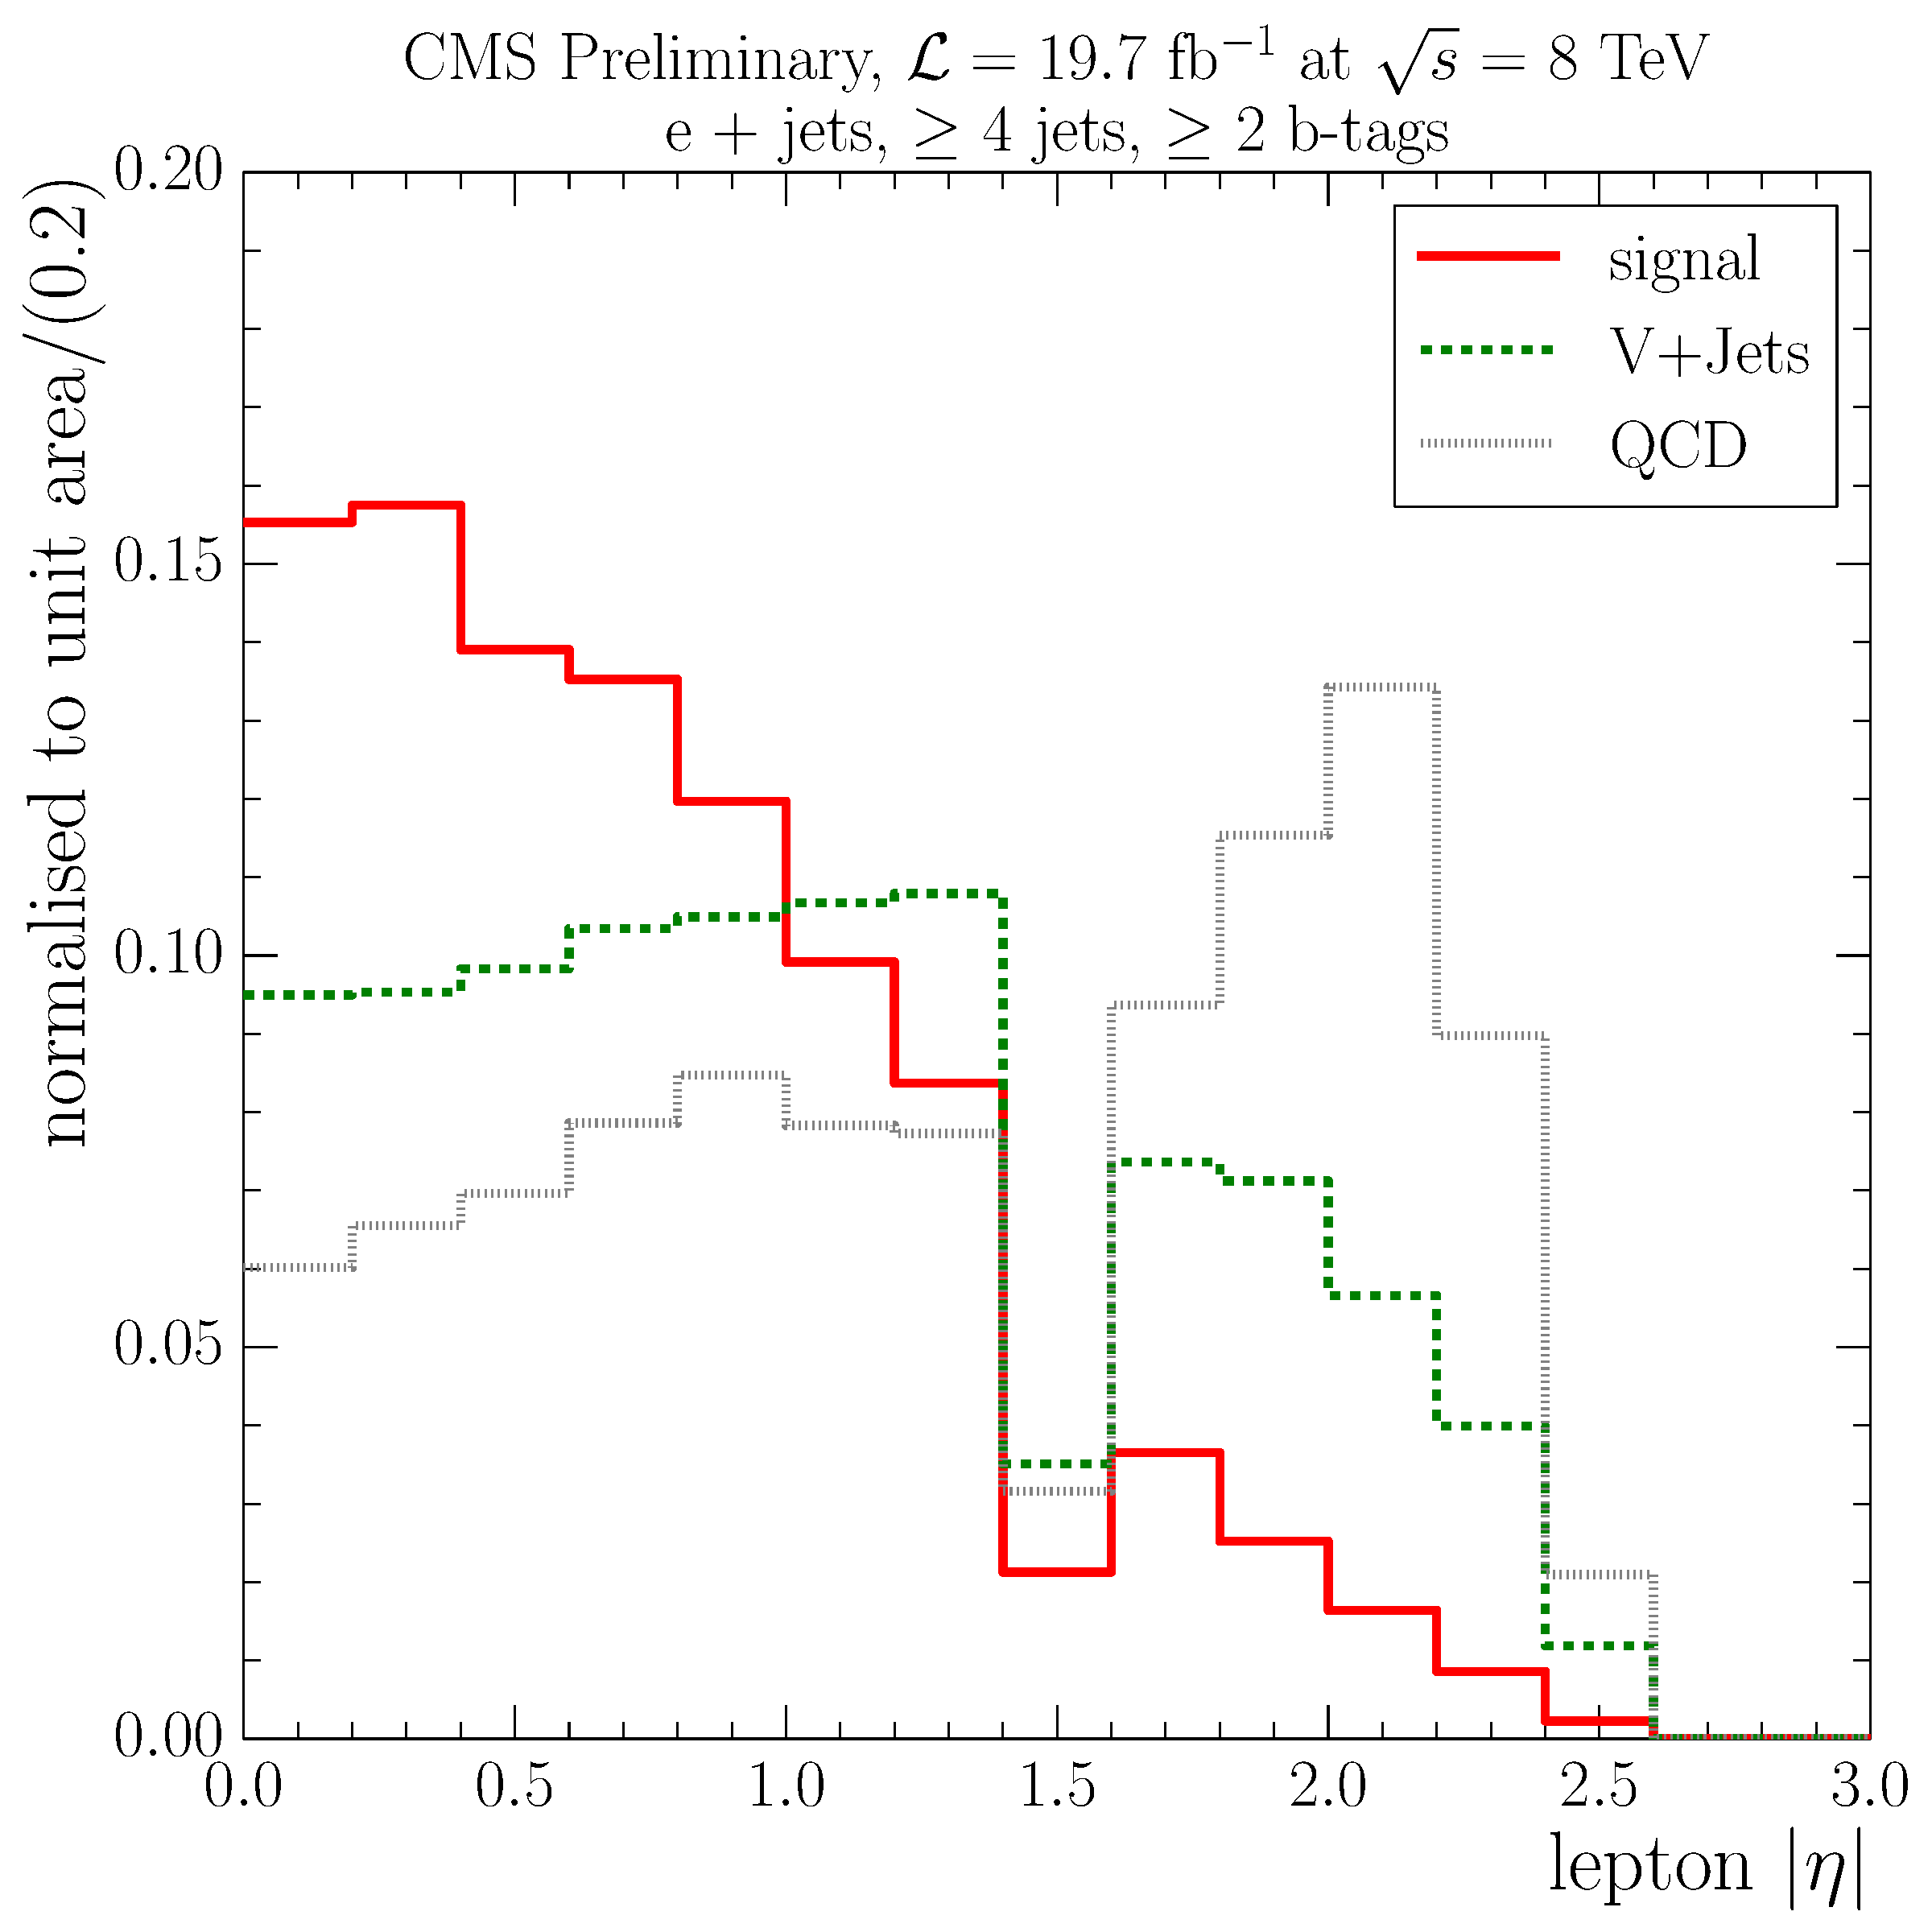
\includegraphics[width=0.3\textwidth]{measurement/ST/central/fit_templates/electron_templates_bin_450-500}}
    {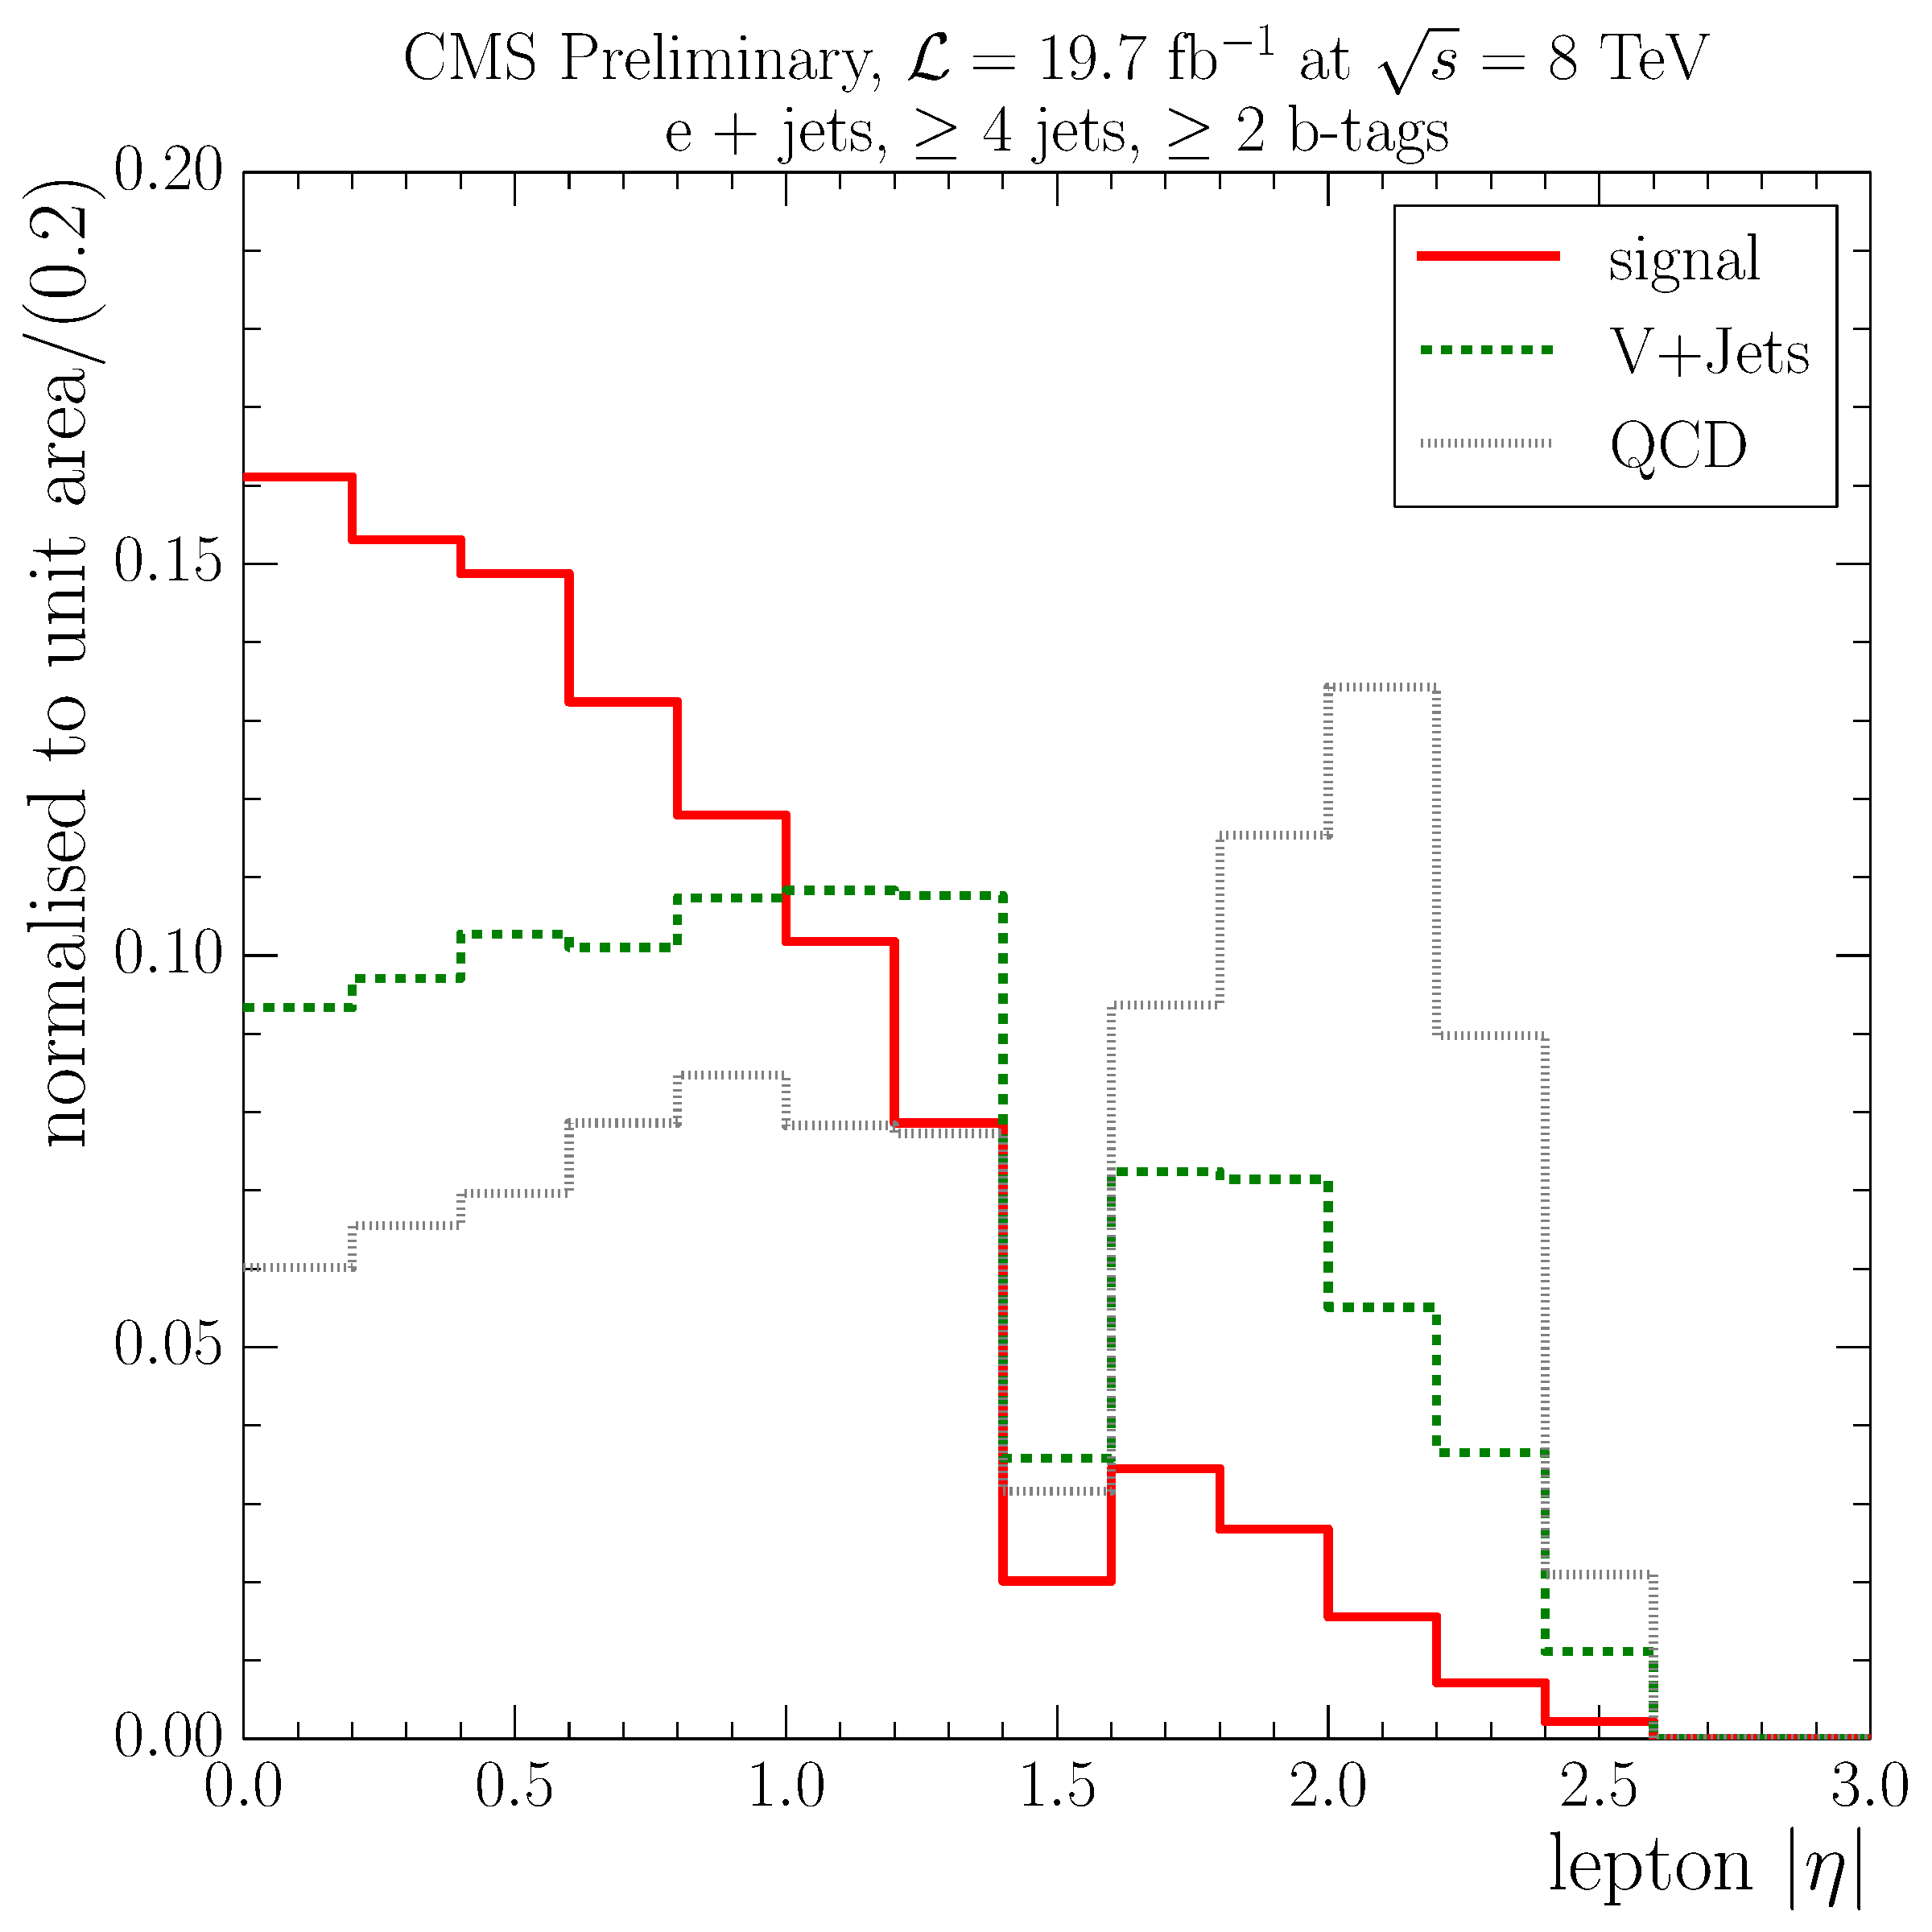
\includegraphics[width=0.3\textwidth]{measurement/ST/central/fit_templates/electron_templates_bin_500-580}}
    {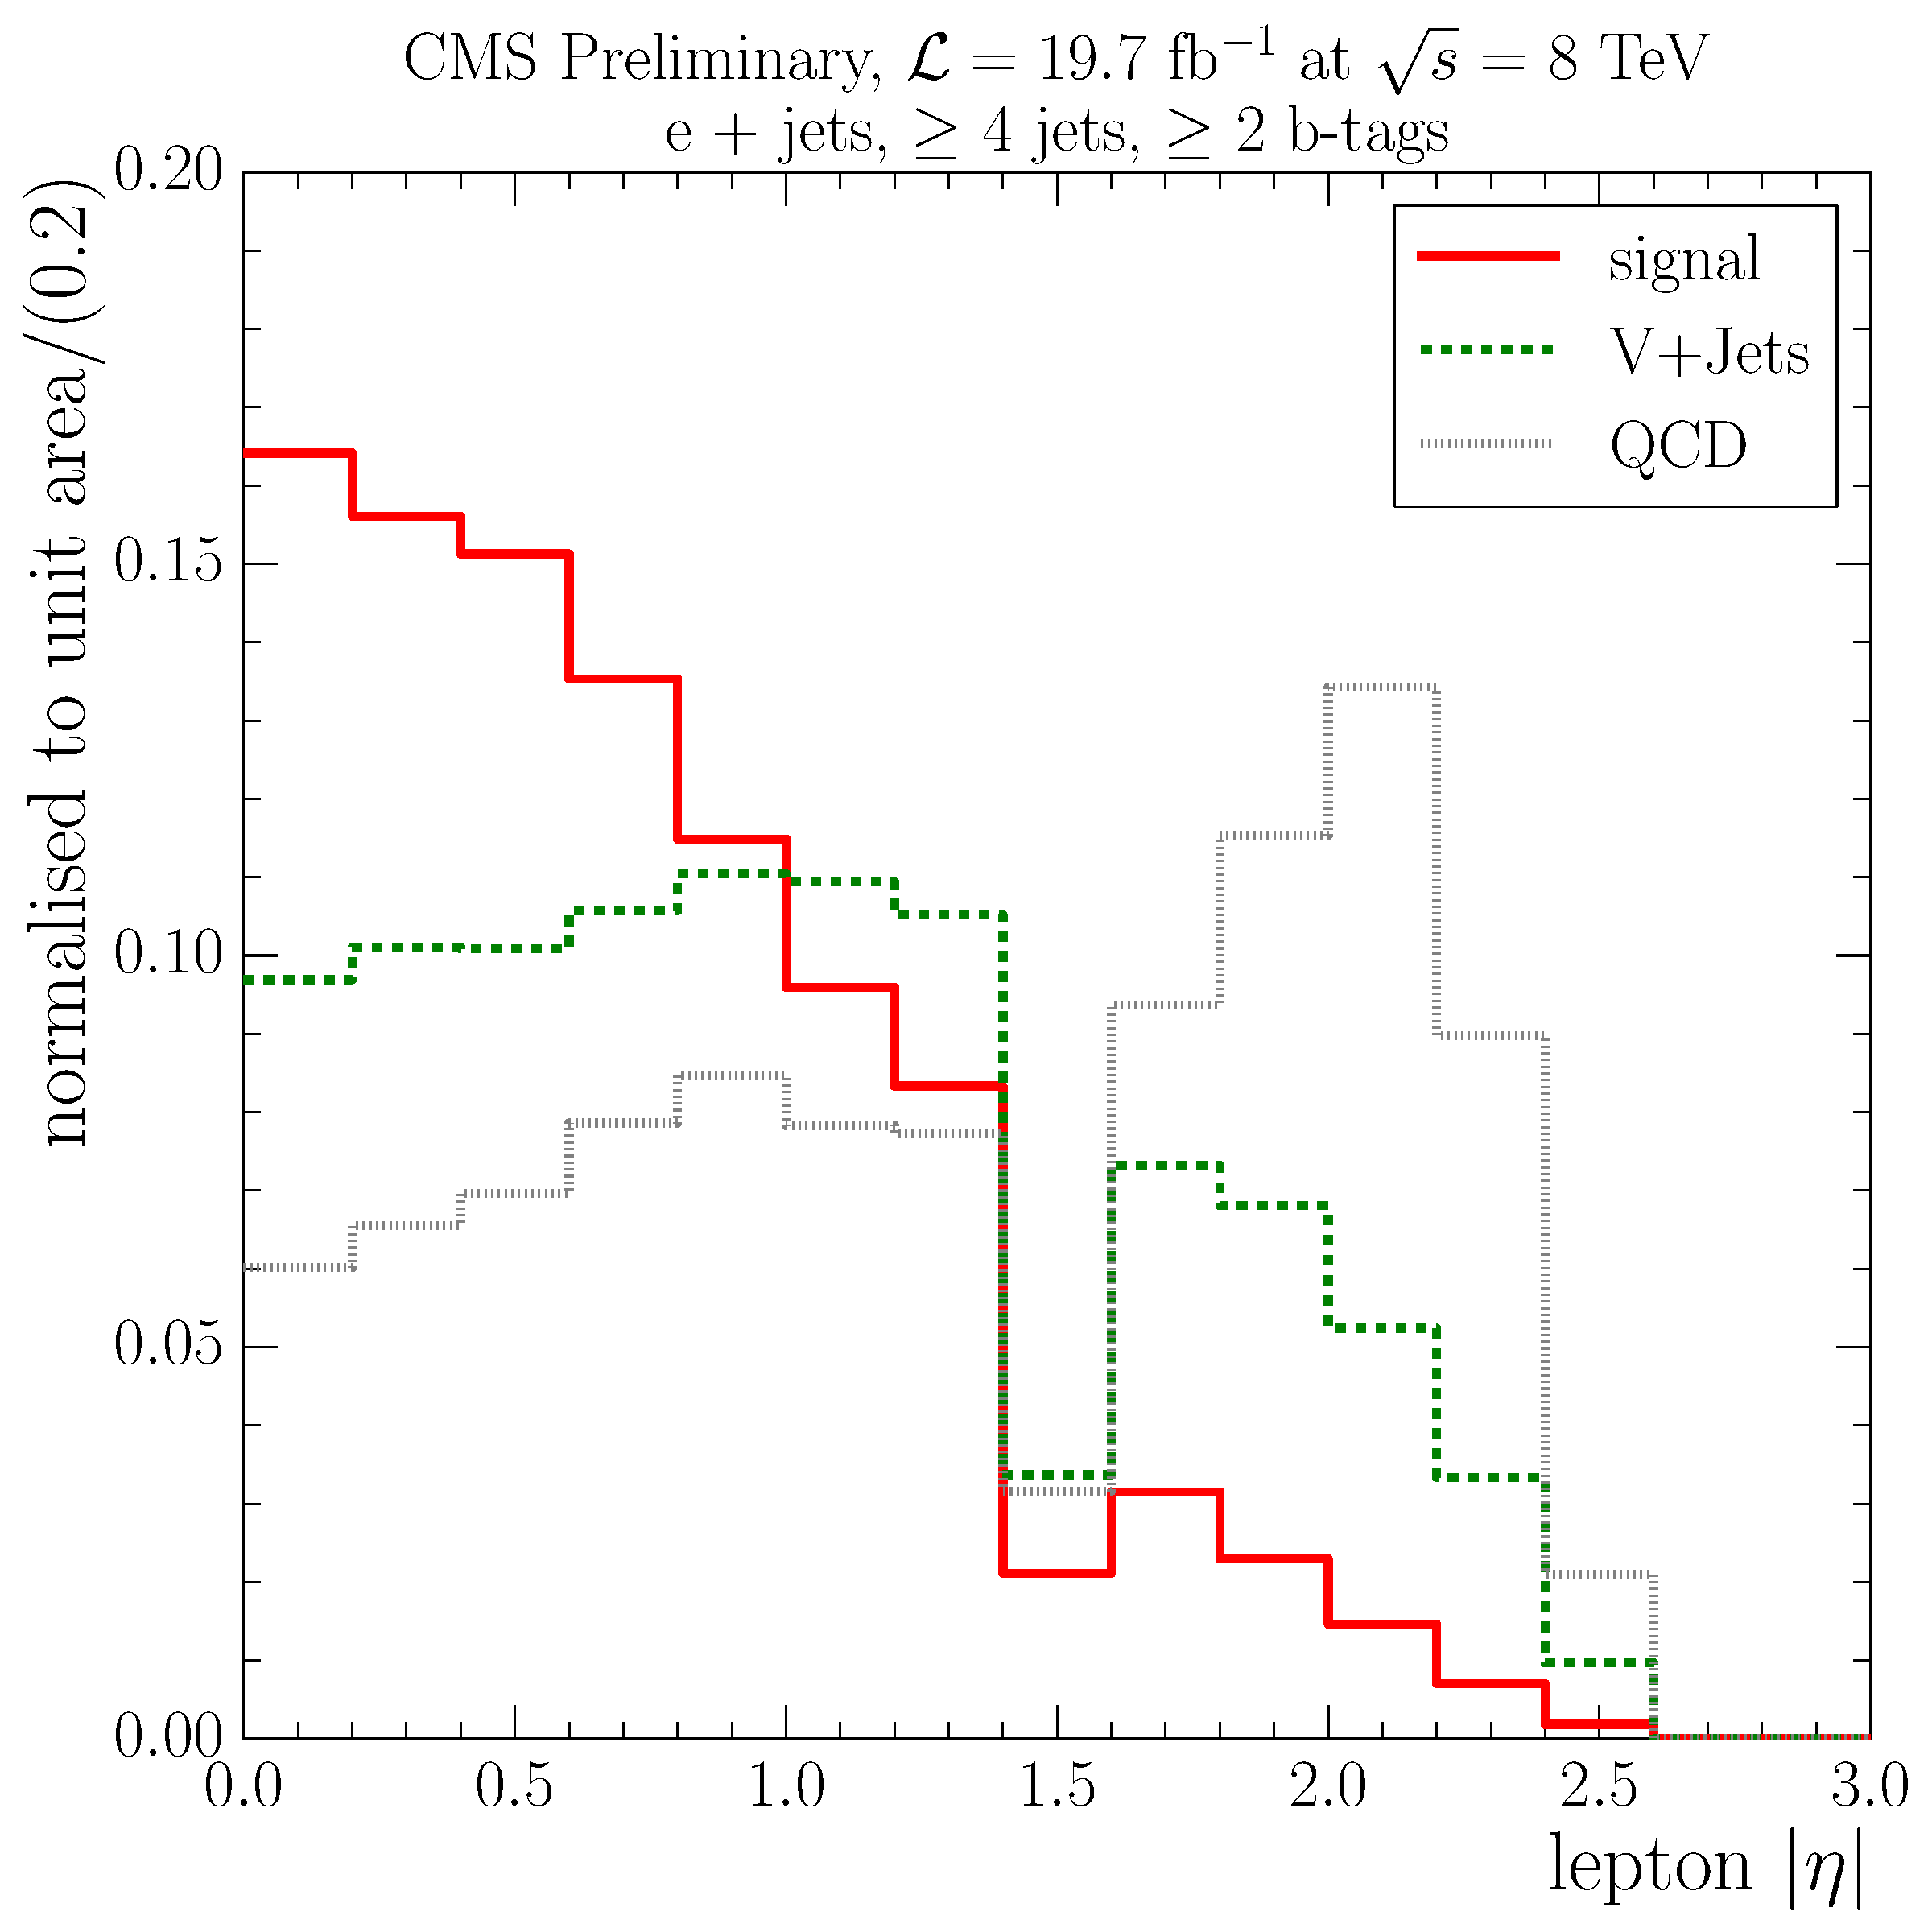
\includegraphics[width=0.3\textwidth]{measurement/ST/central/fit_templates/electron_templates_bin_580-700}}\\
    {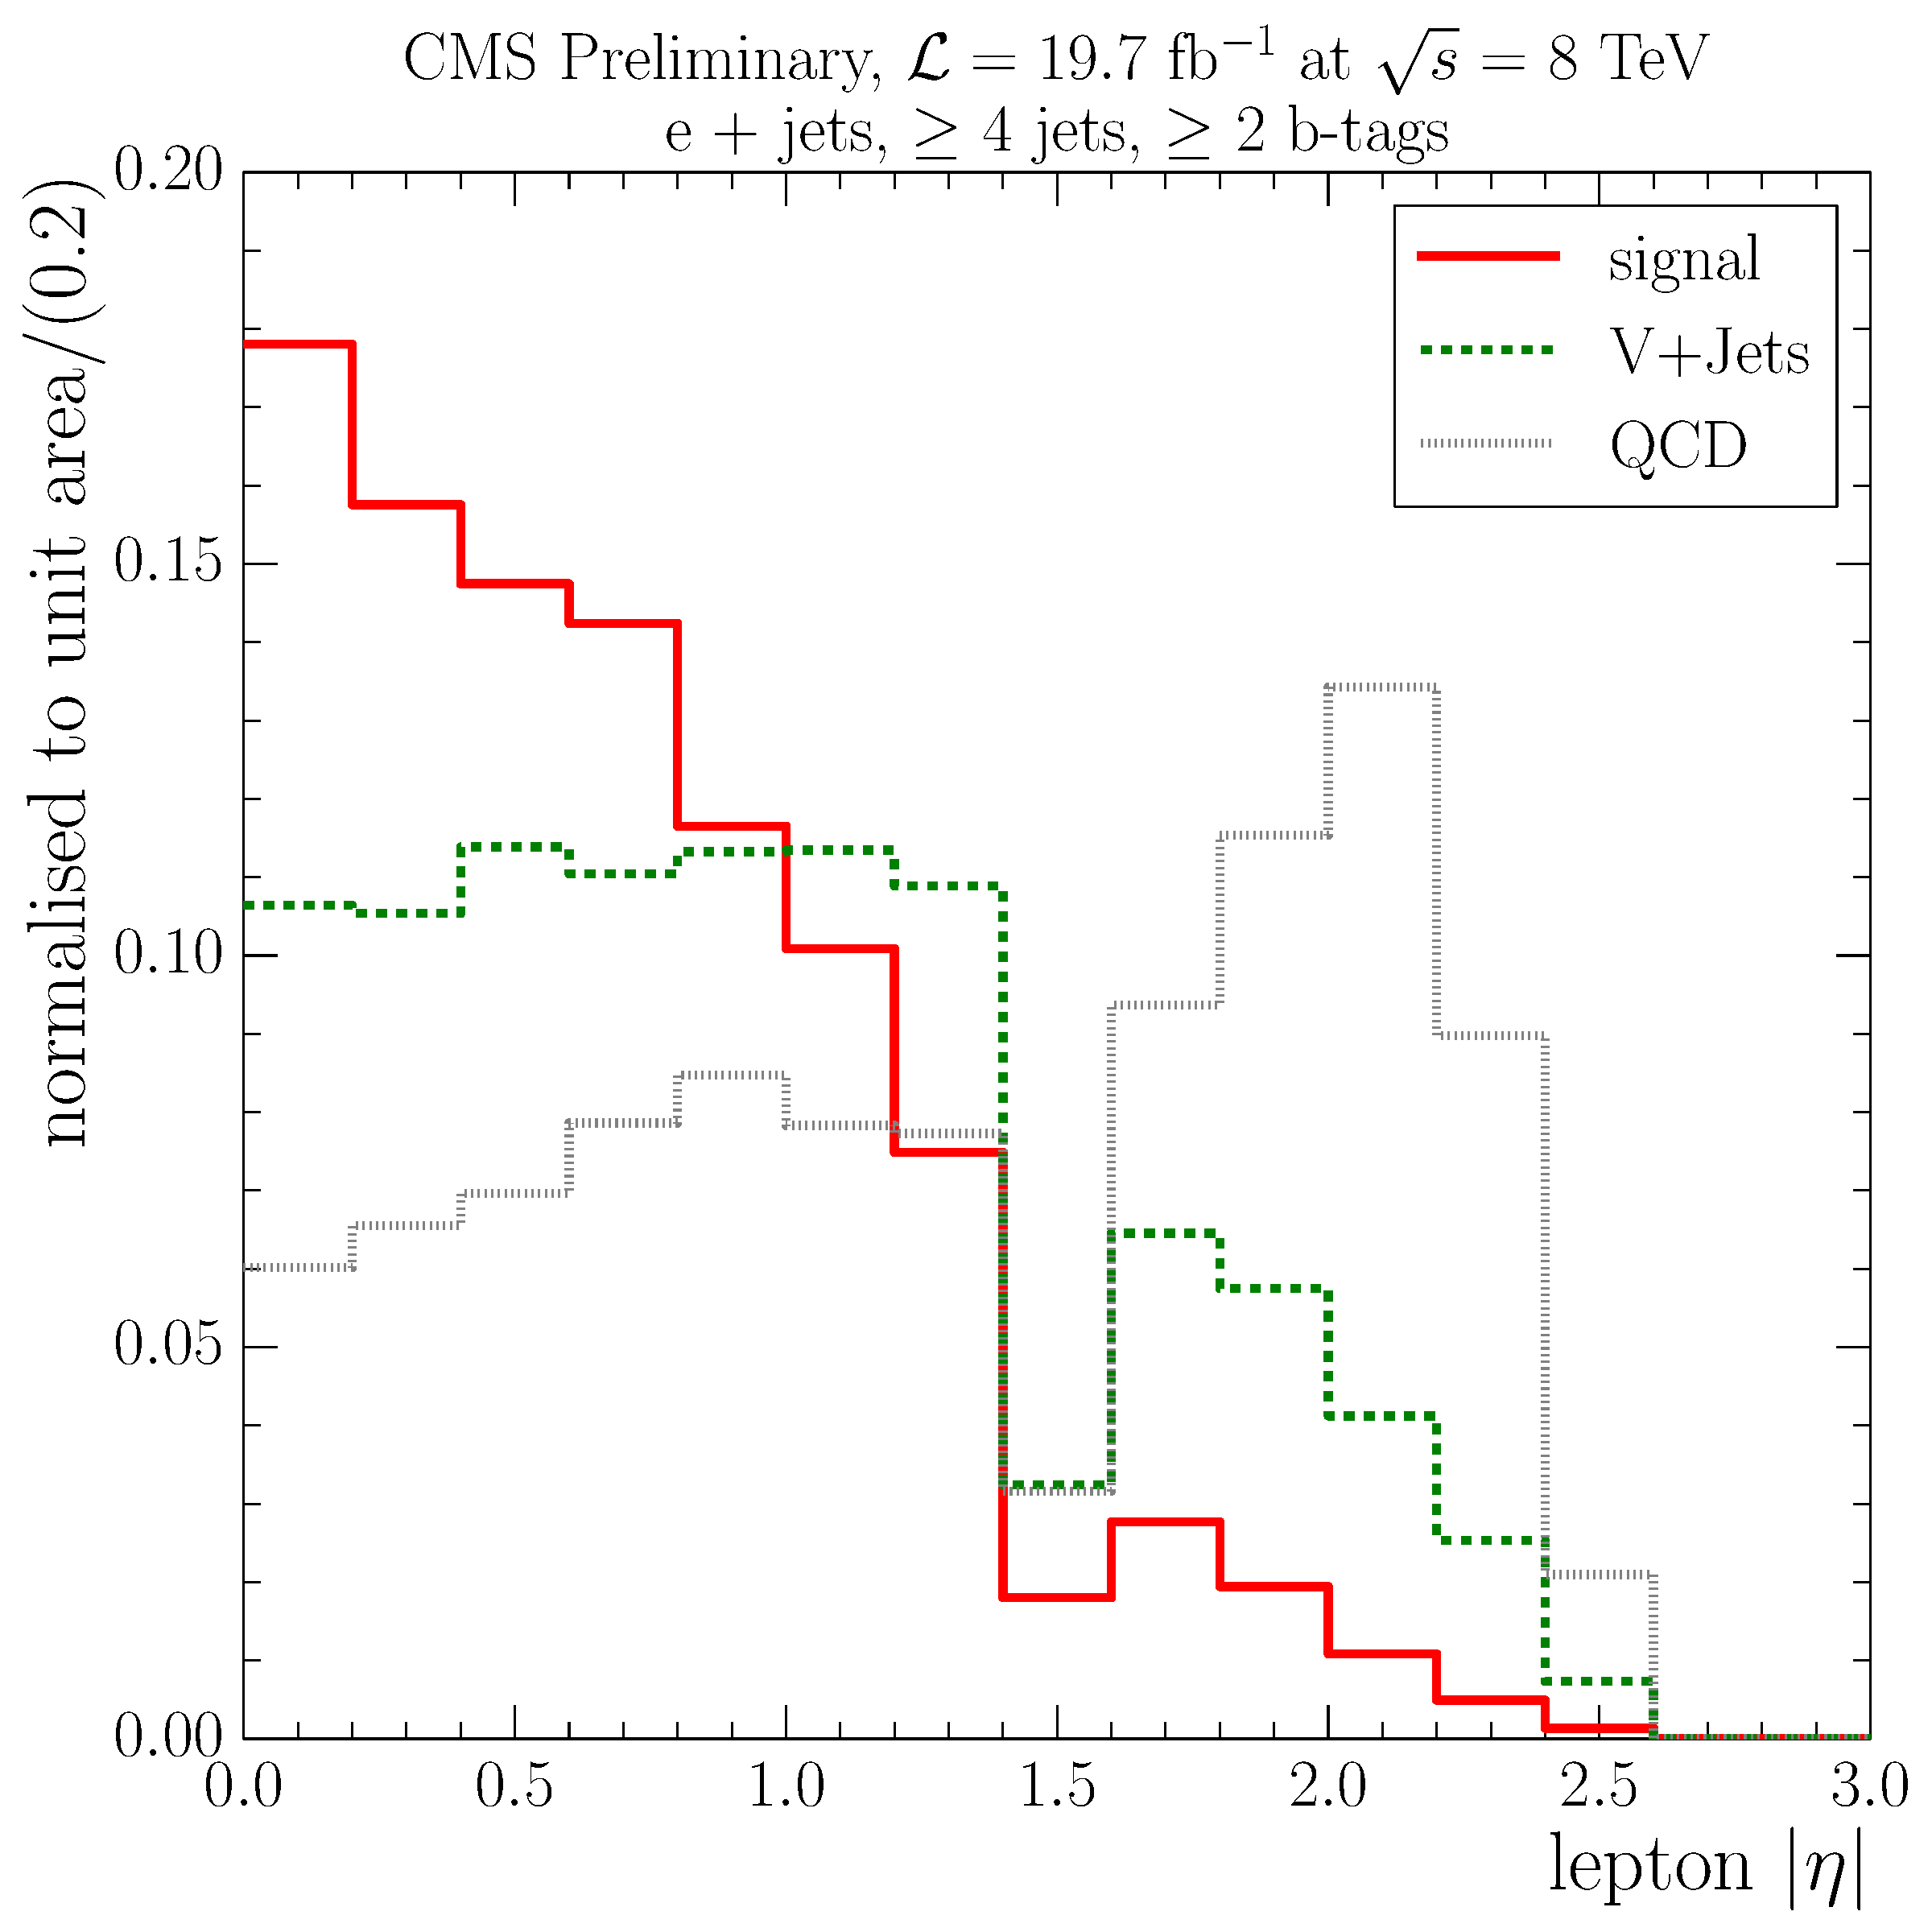
\includegraphics[width=0.3\textwidth]{measurement/ST/central/fit_templates/electron_templates_bin_700-inf}}
    \caption{Electron $\abs \eta$ templates for the fit in different bins of \ST,
    from top left to bottom right: \SIrange{0}{350}{\GeV}, \SIrange{350}{400}{\GeV},
    \SIrange{400}{450}{\GeV}, \SIrange{450}{500}{\GeV}, \SIrange{500}{580}{\GeV},
    \SIrange{580}{700}{\GeV} and $\geq \SI{700}{\GeV}$.}
    \label{fig:fit_tempaltes_ST_electron}
\end{figure}

\begin{figure}[!htbp]
  \centering
    {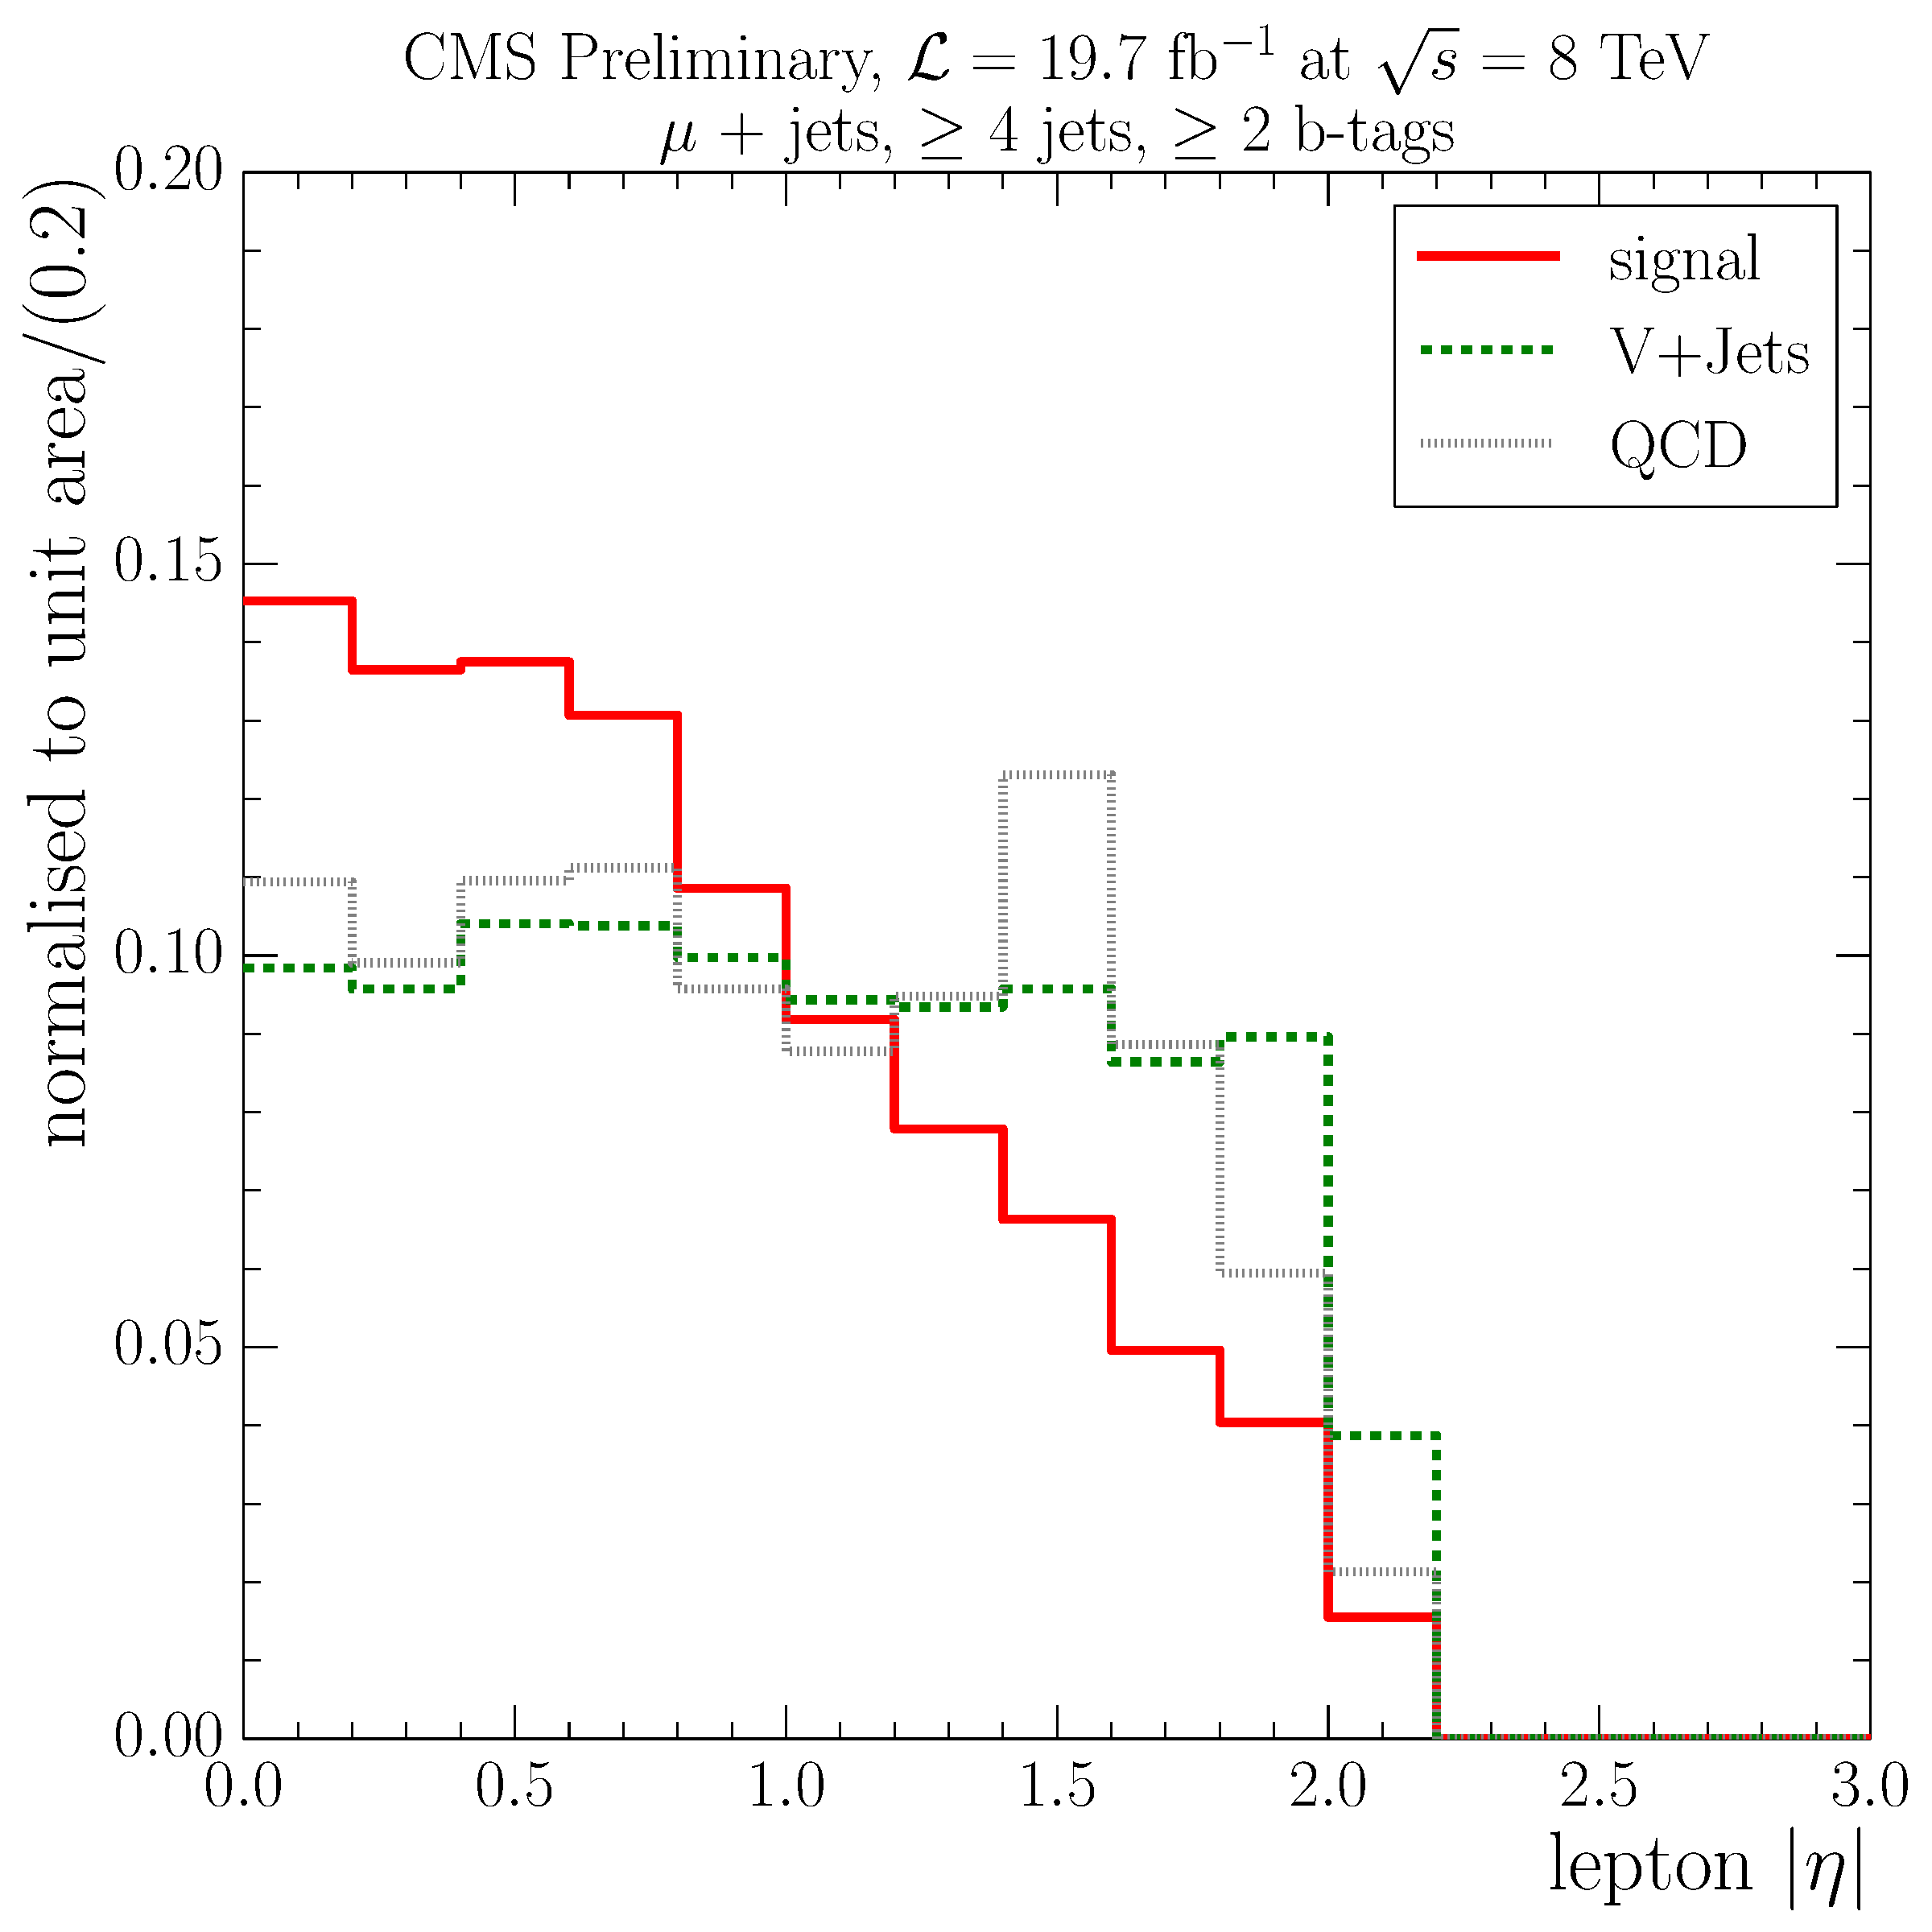
\includegraphics[width=0.3\textwidth]{measurement/ST/central/fit_templates/muon_templates_bin_0-350}}
    {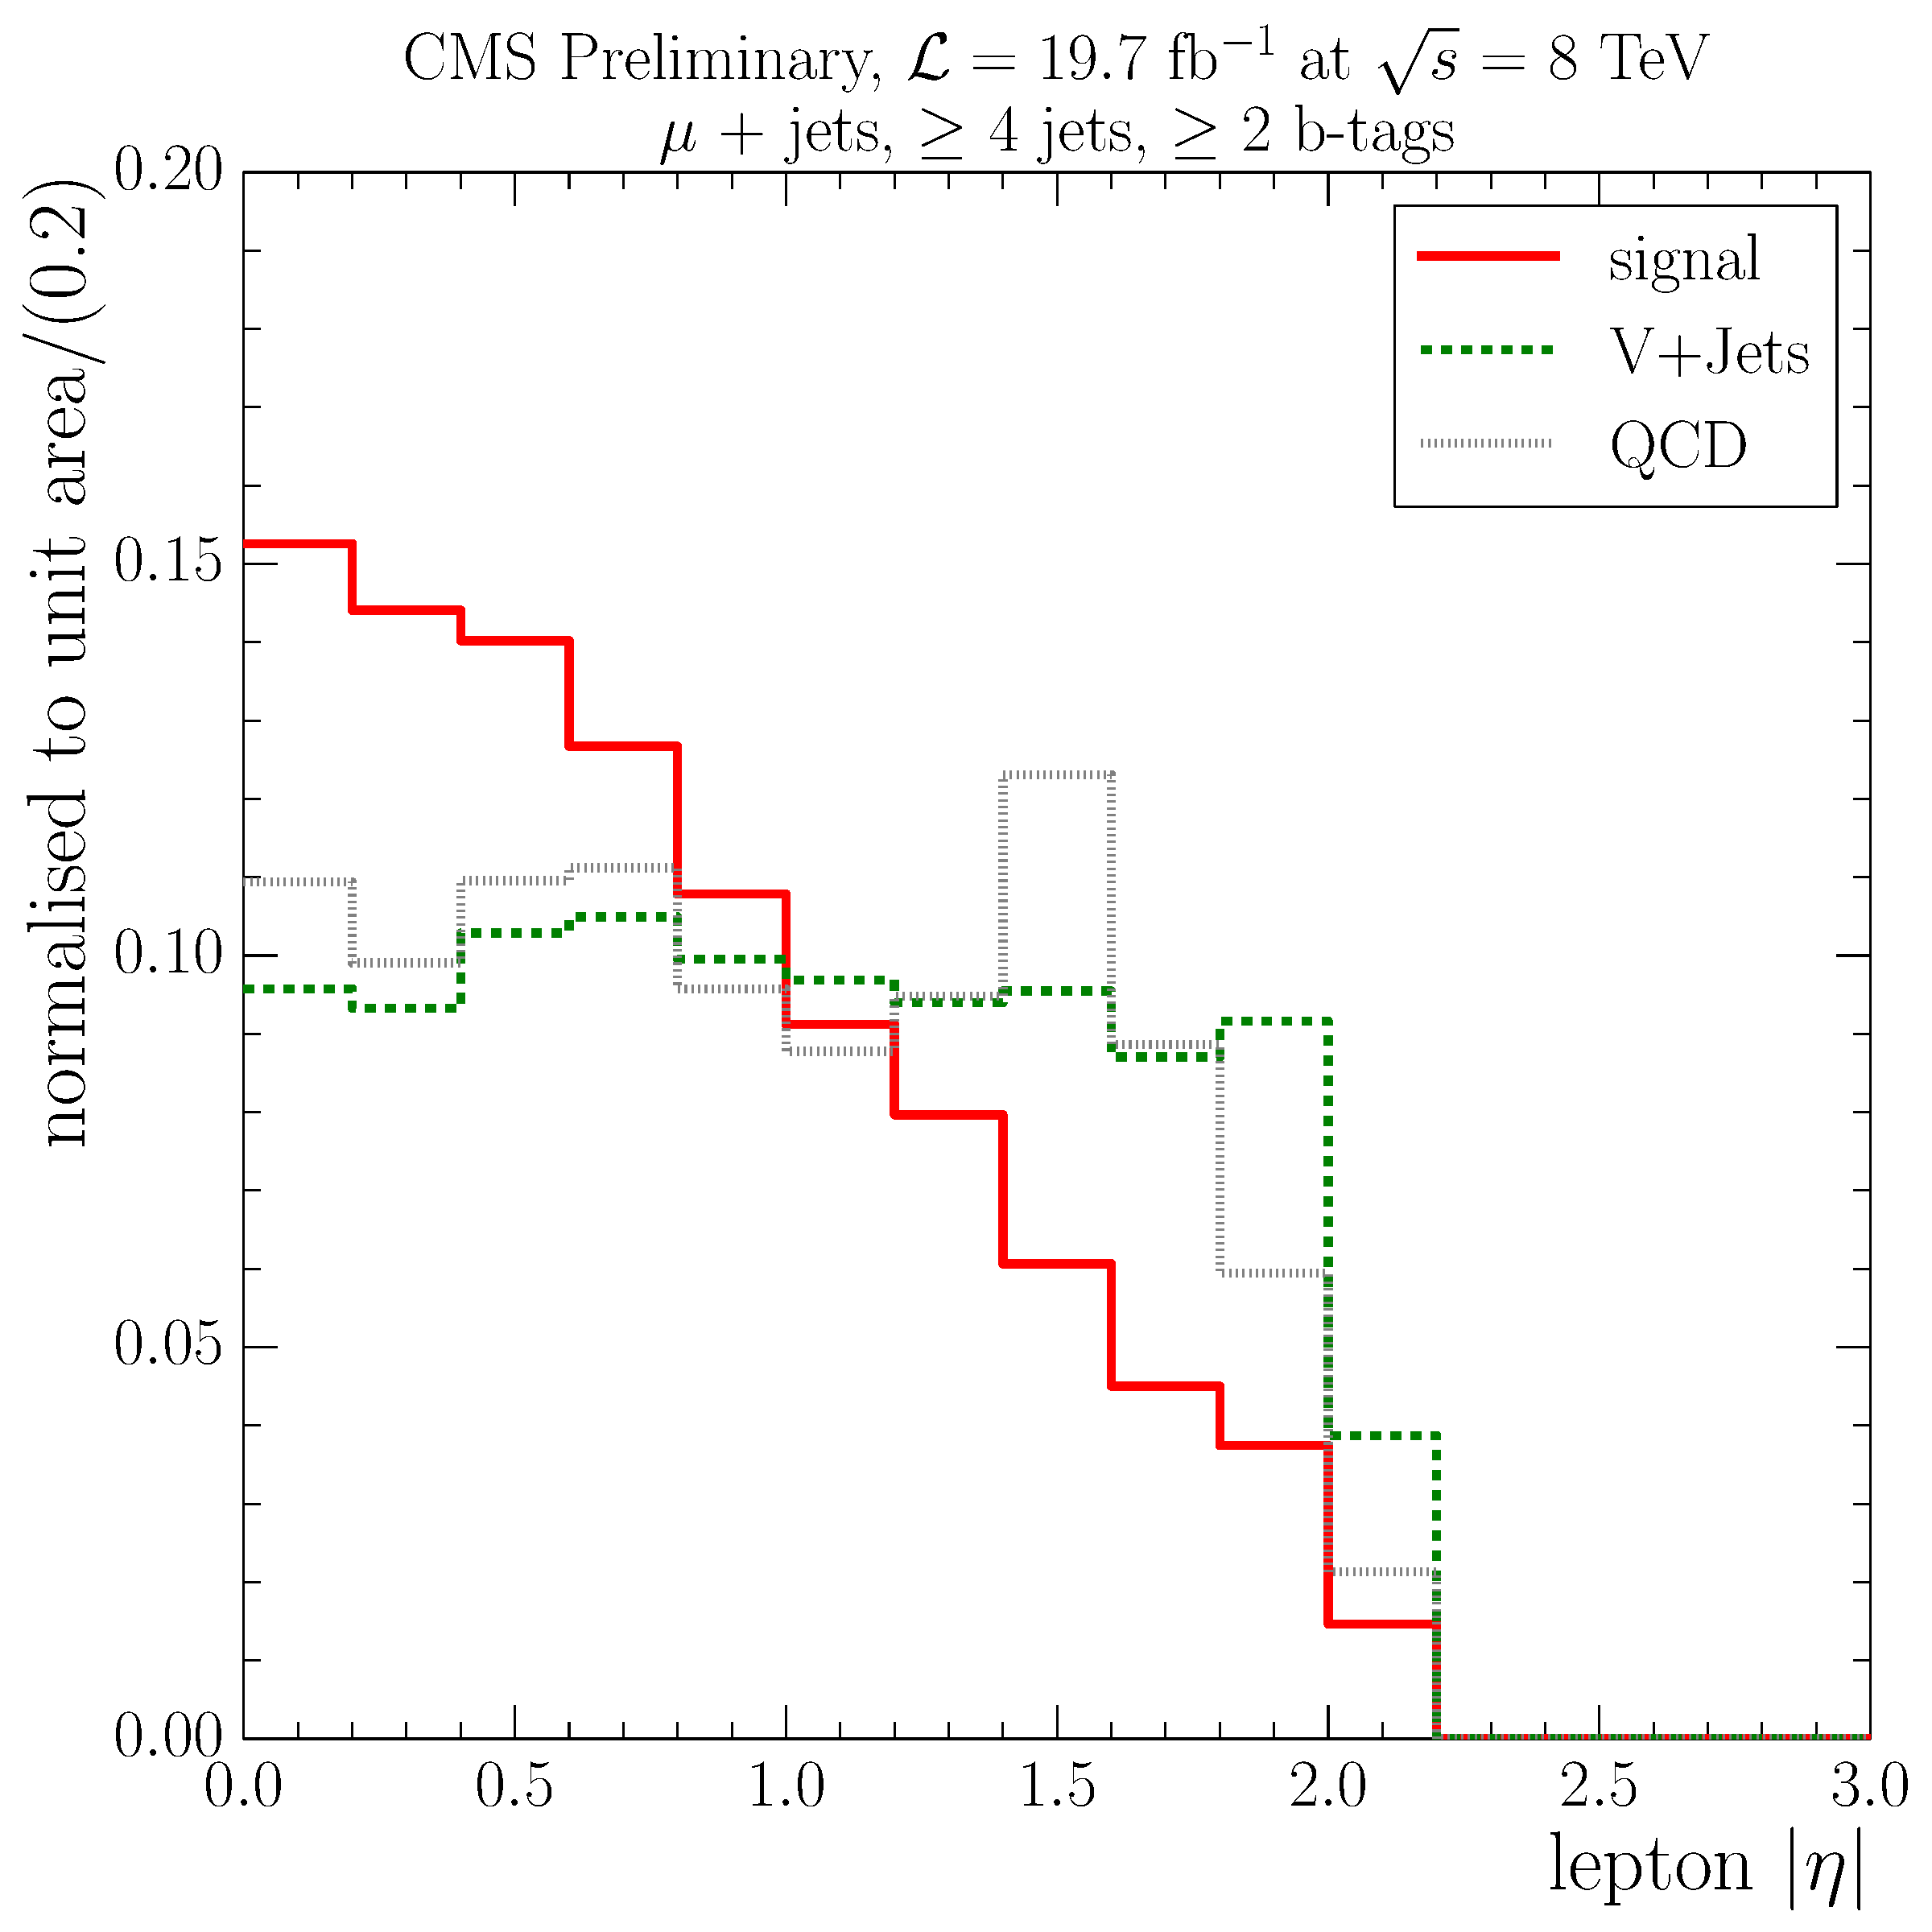
\includegraphics[width=0.3\textwidth]{measurement/ST/central/fit_templates/muon_templates_bin_350-400}}
    {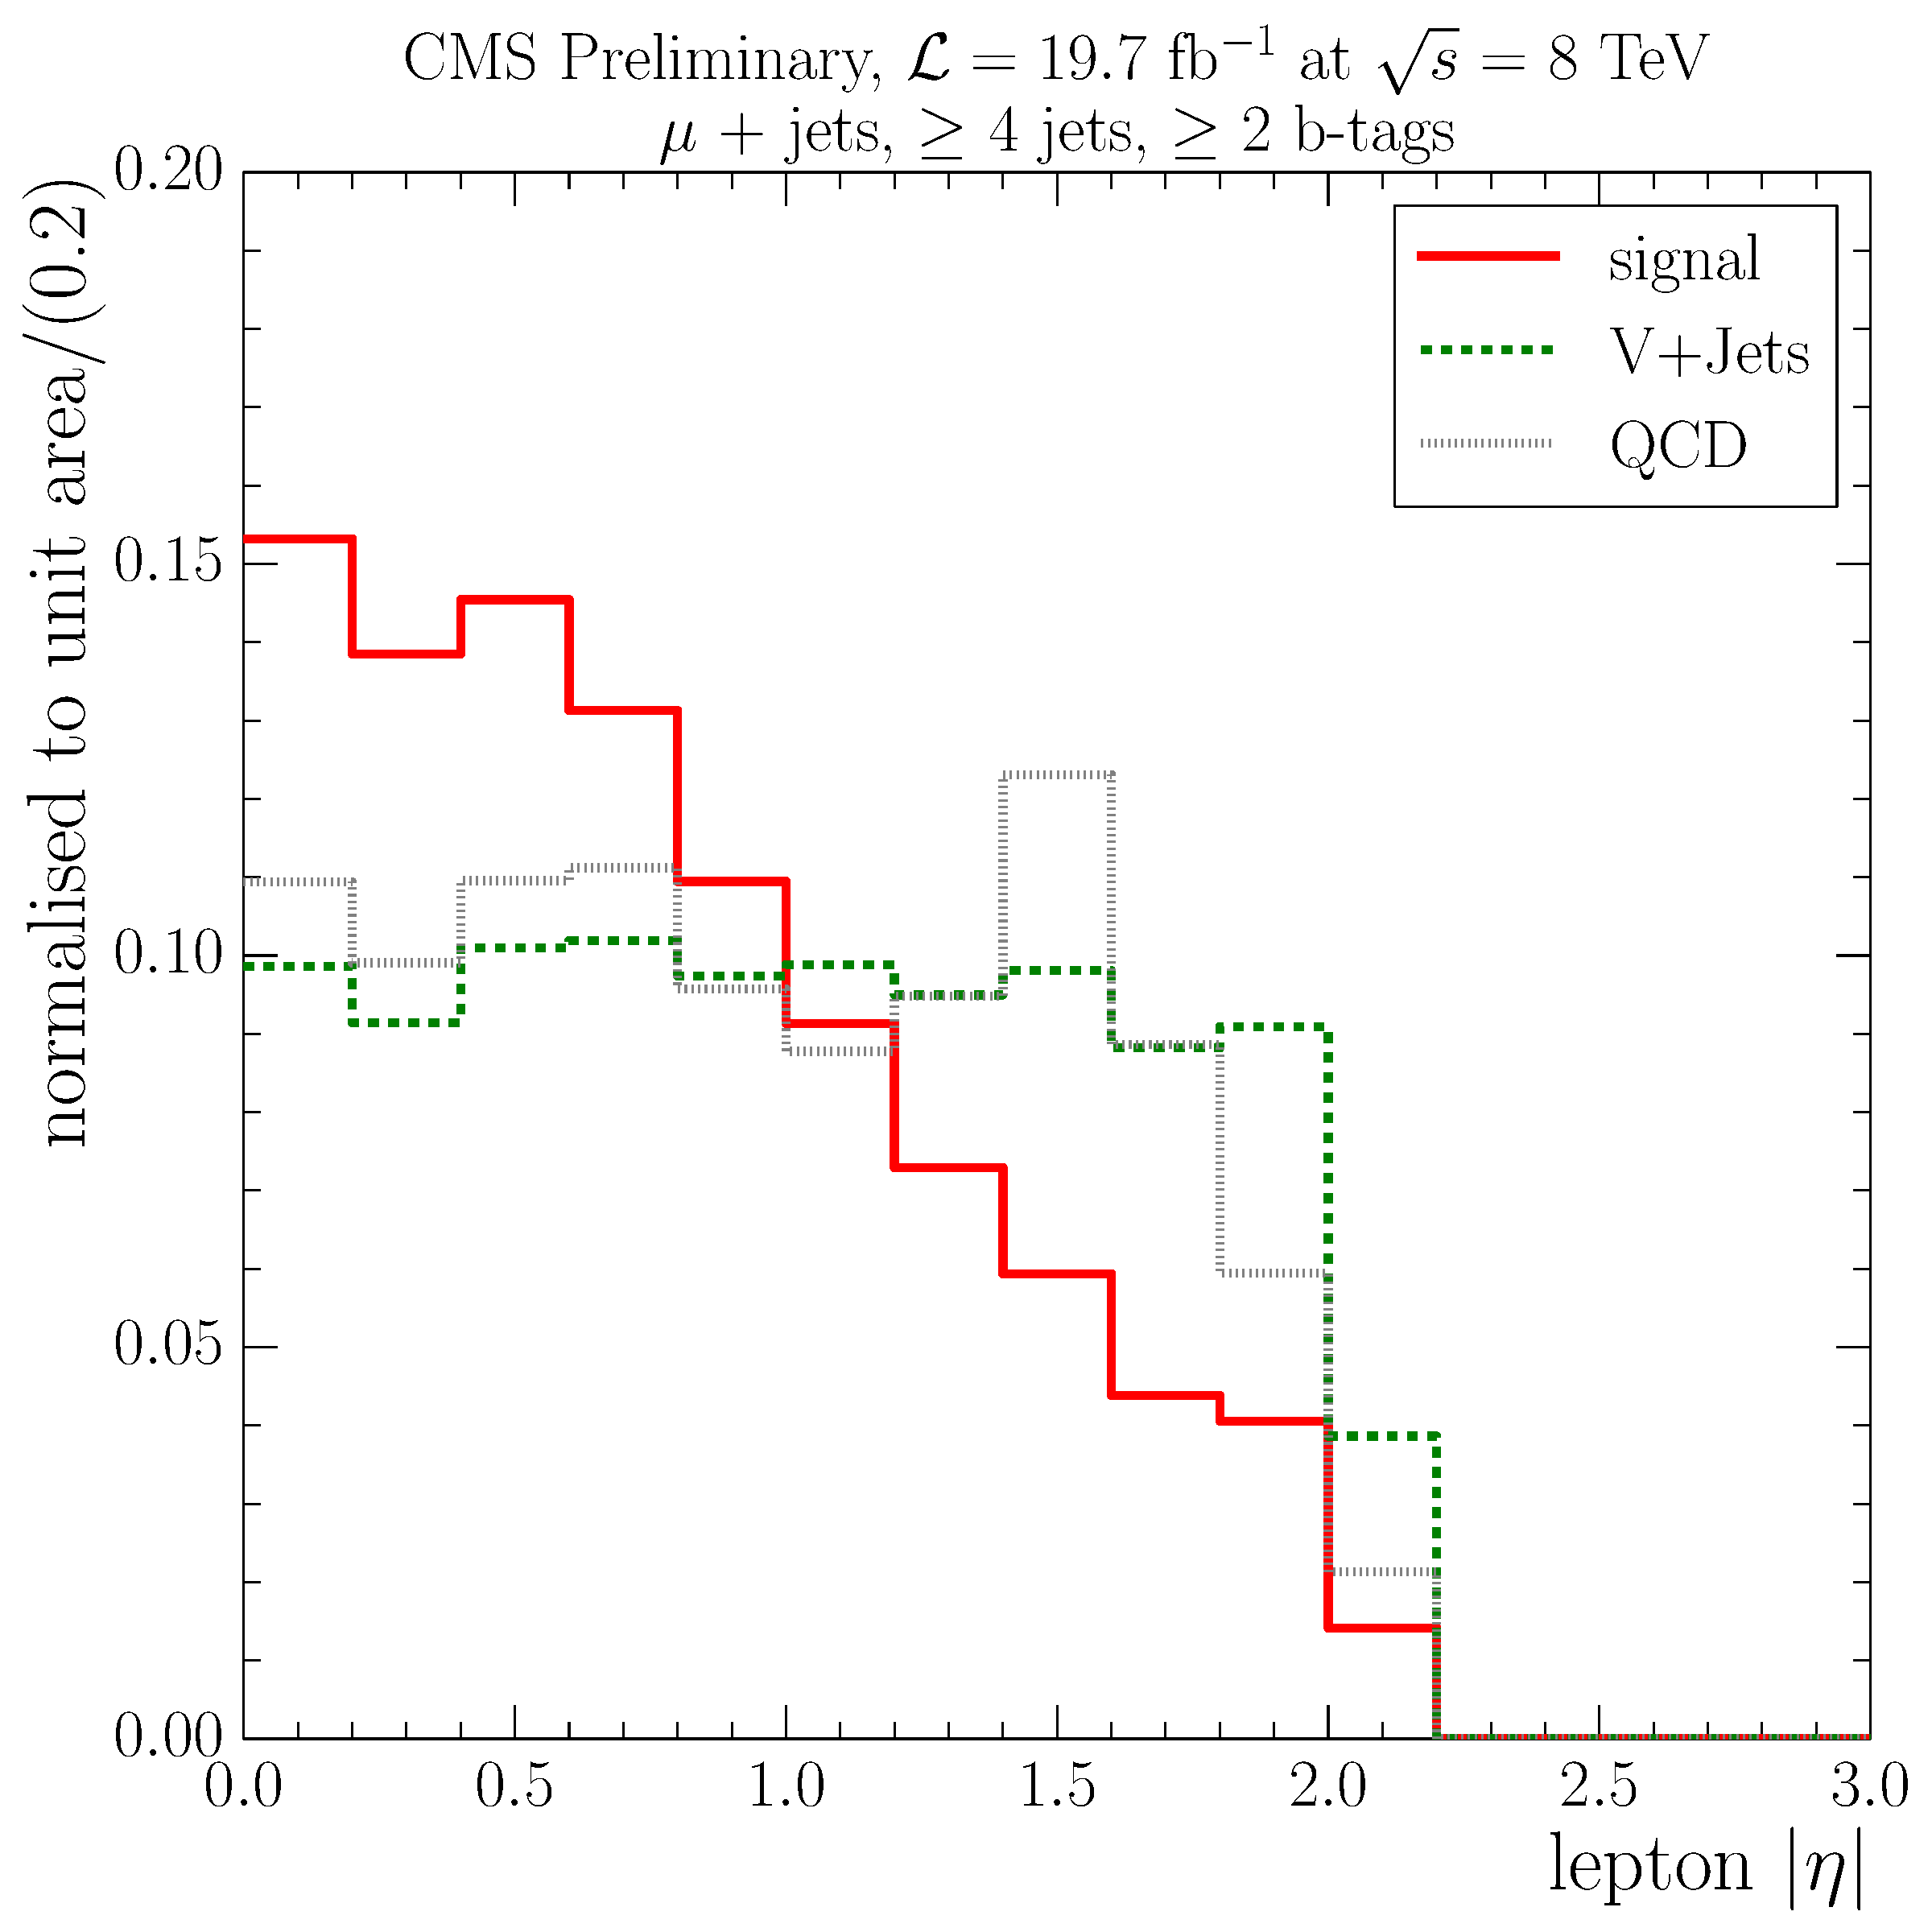
\includegraphics[width=0.3\textwidth]{measurement/ST/central/fit_templates/muon_templates_bin_400-450}}\\
    {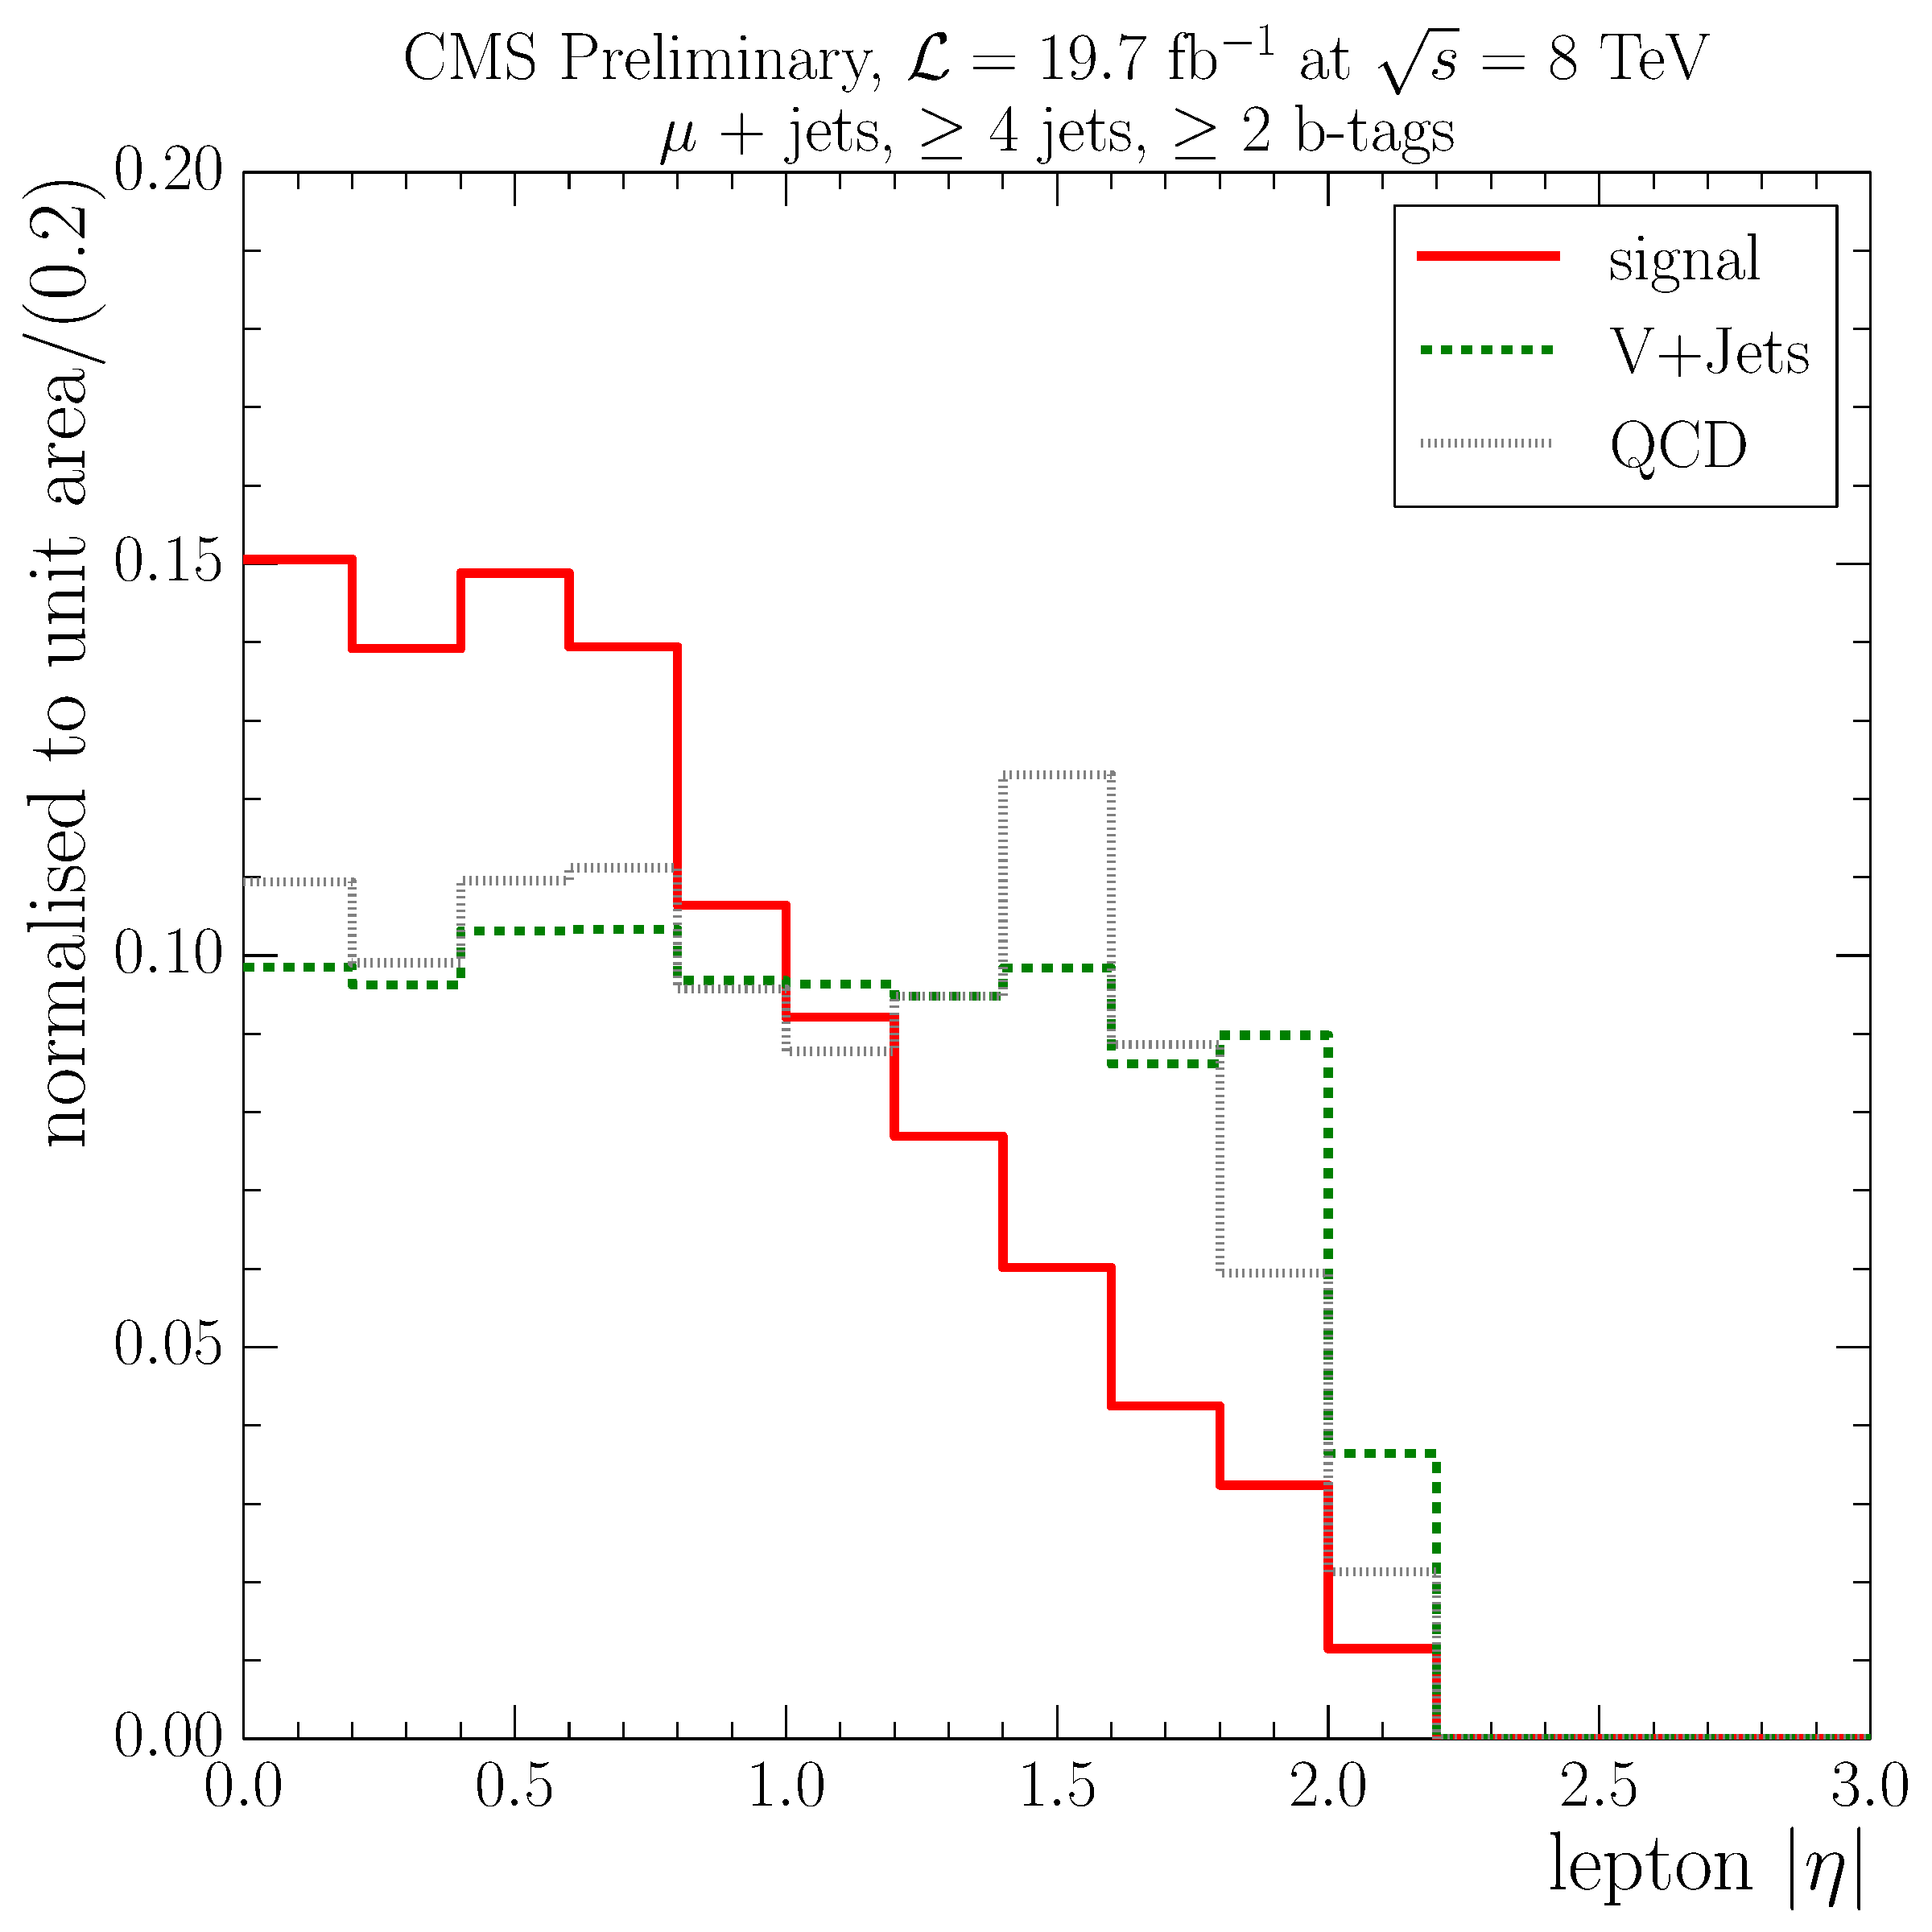
\includegraphics[width=0.3\textwidth]{measurement/ST/central/fit_templates/muon_templates_bin_450-500}}
    {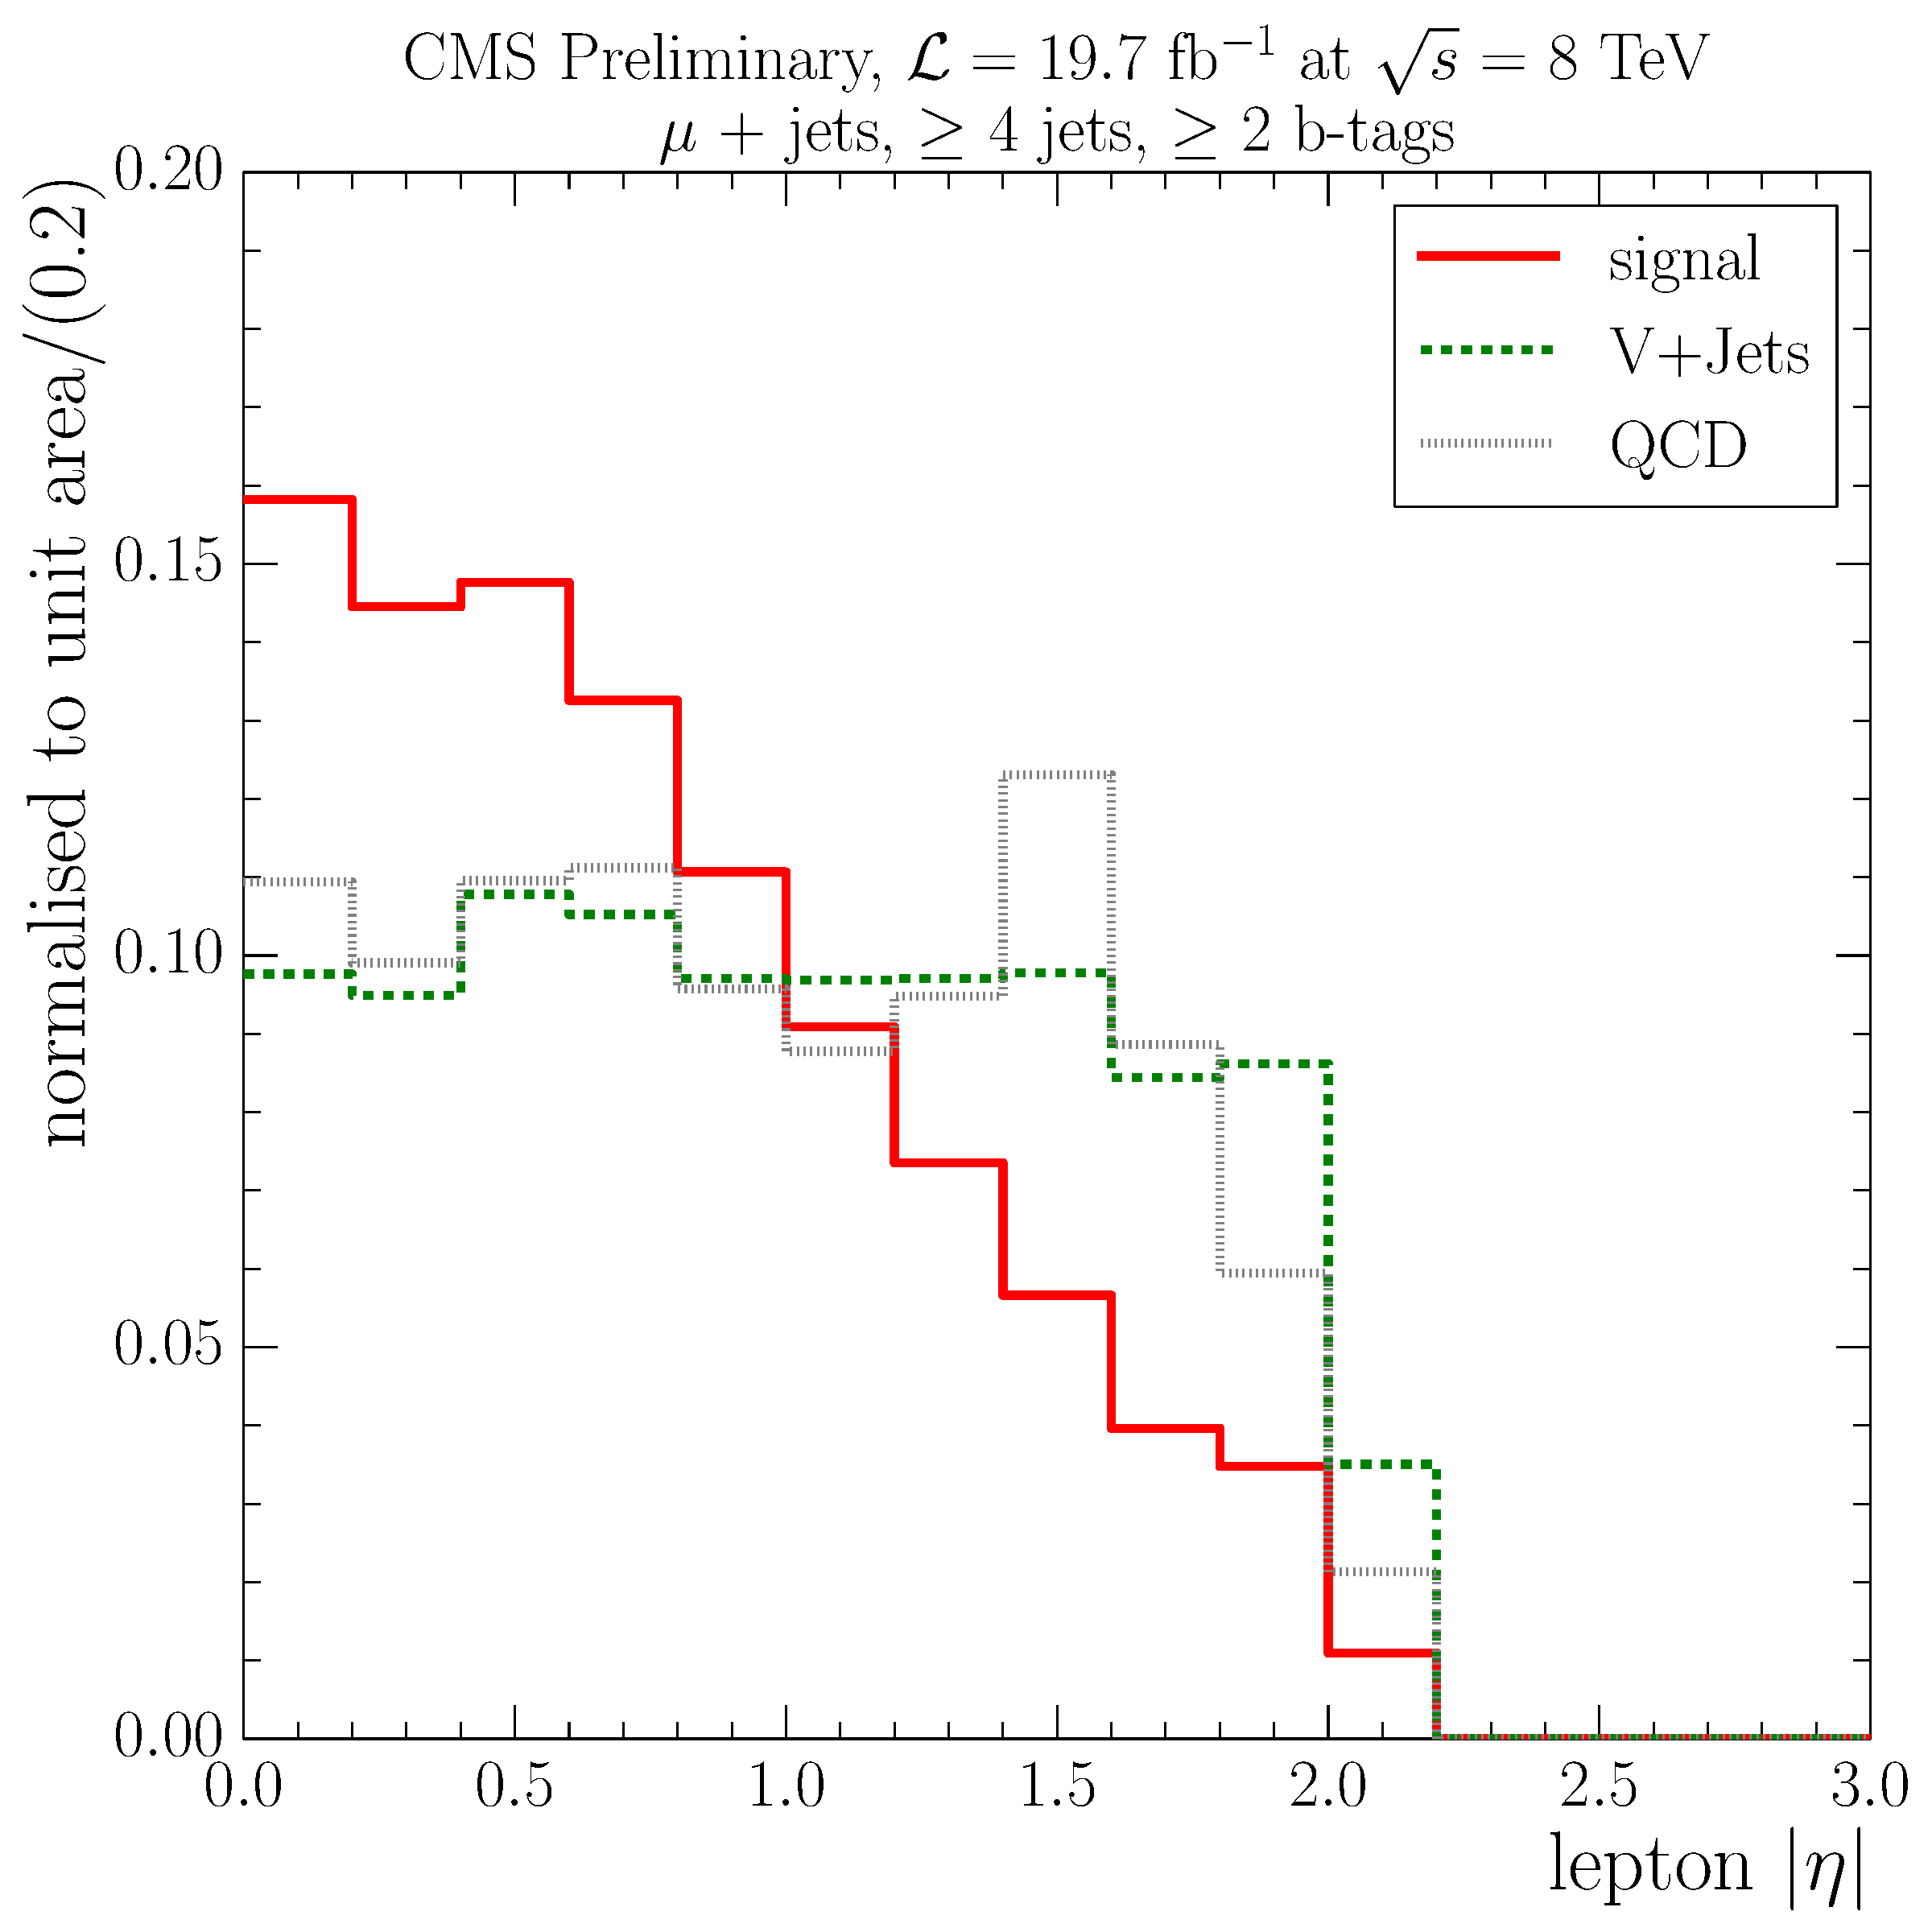
\includegraphics[width=0.3\textwidth]{measurement/ST/central/fit_templates/muon_templates_bin_500-580}}
    {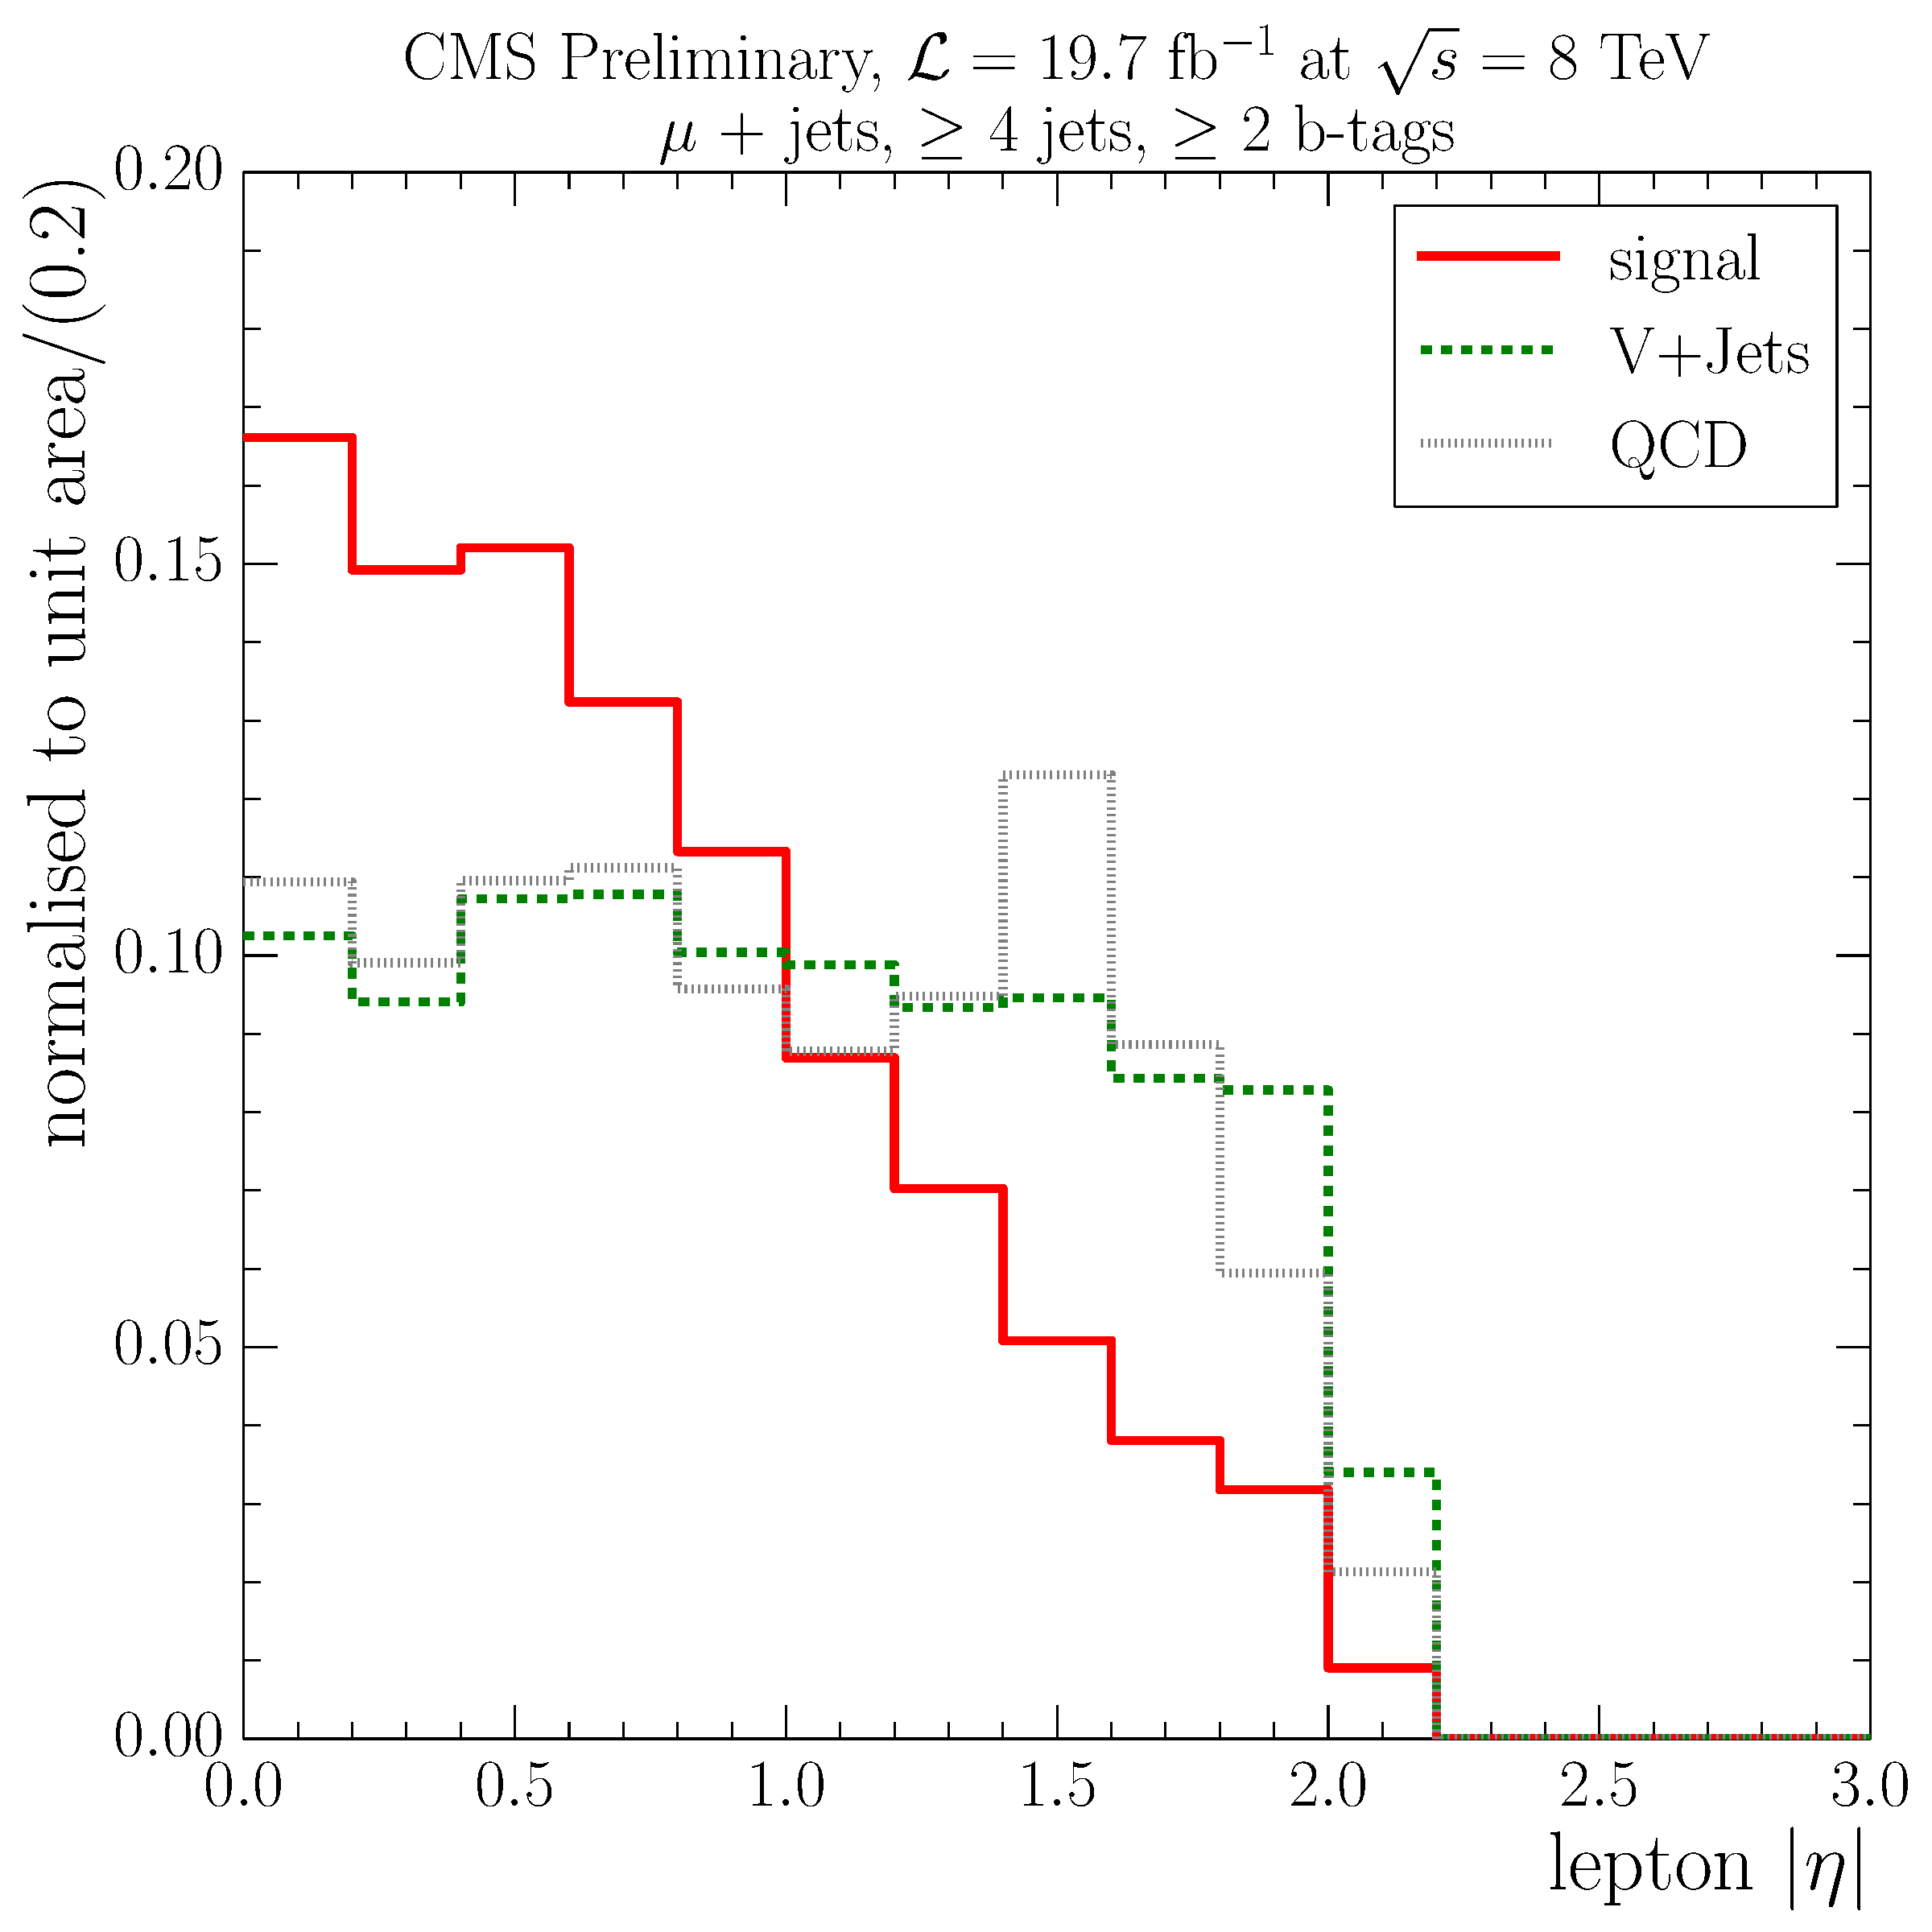
\includegraphics[width=0.3\textwidth]{measurement/ST/central/fit_templates/muon_templates_bin_580-700}}\\
    {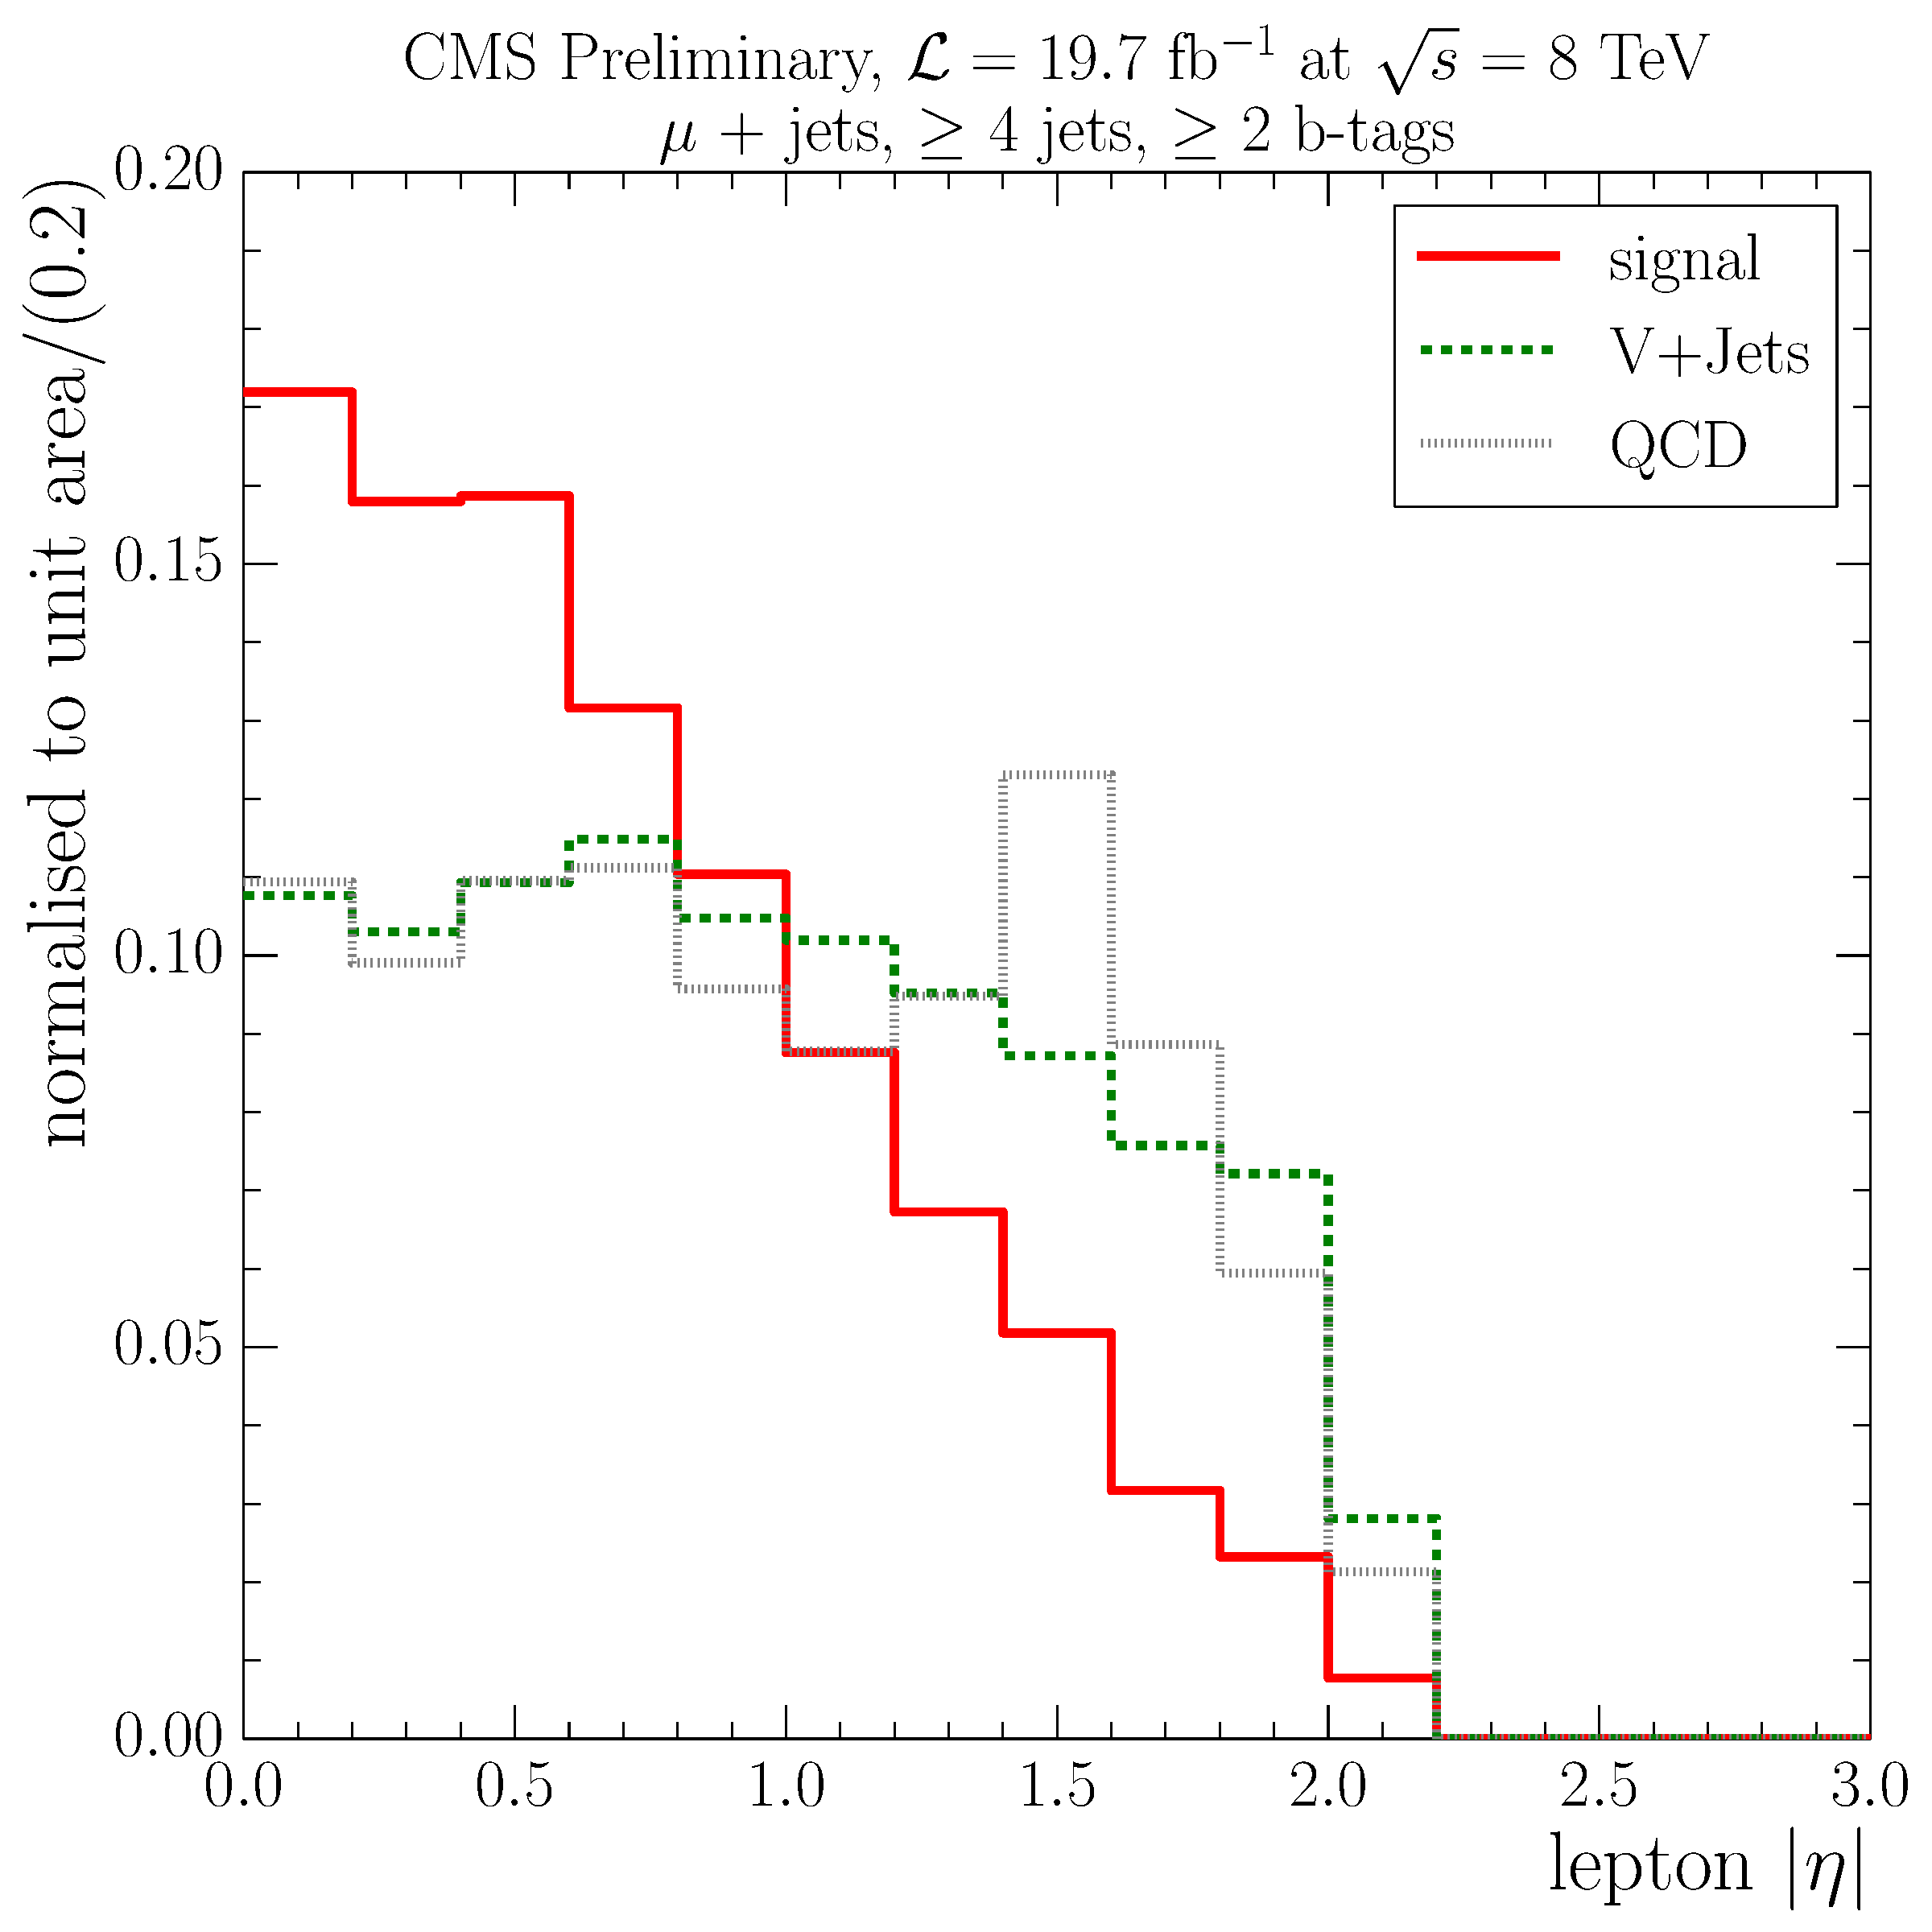
\includegraphics[width=0.3\textwidth]{measurement/ST/central/fit_templates/muon_templates_bin_700-inf}}
    \caption{Electron $\abs \eta$ templates for the fit in different bins of \ST,
    from top left to bottom right: \SIrange{0}{350}{\GeV}, \SIrange{350}{400}{\GeV},
    \SIrange{400}{450}{\GeV}, \SIrange{450}{500}{\GeV}, \SIrange{500}{580}{\GeV},
    \SIrange{580}{700}{\GeV} and $\geq \SI{700}{\GeV}$.}
    \label{fig:fit_templates_ST_muon}
\end{figure}

\newpage
\section*{\WPT variable}

\begin{figure}[!htbp]
  \centering
    \hspace*{\fill}
    {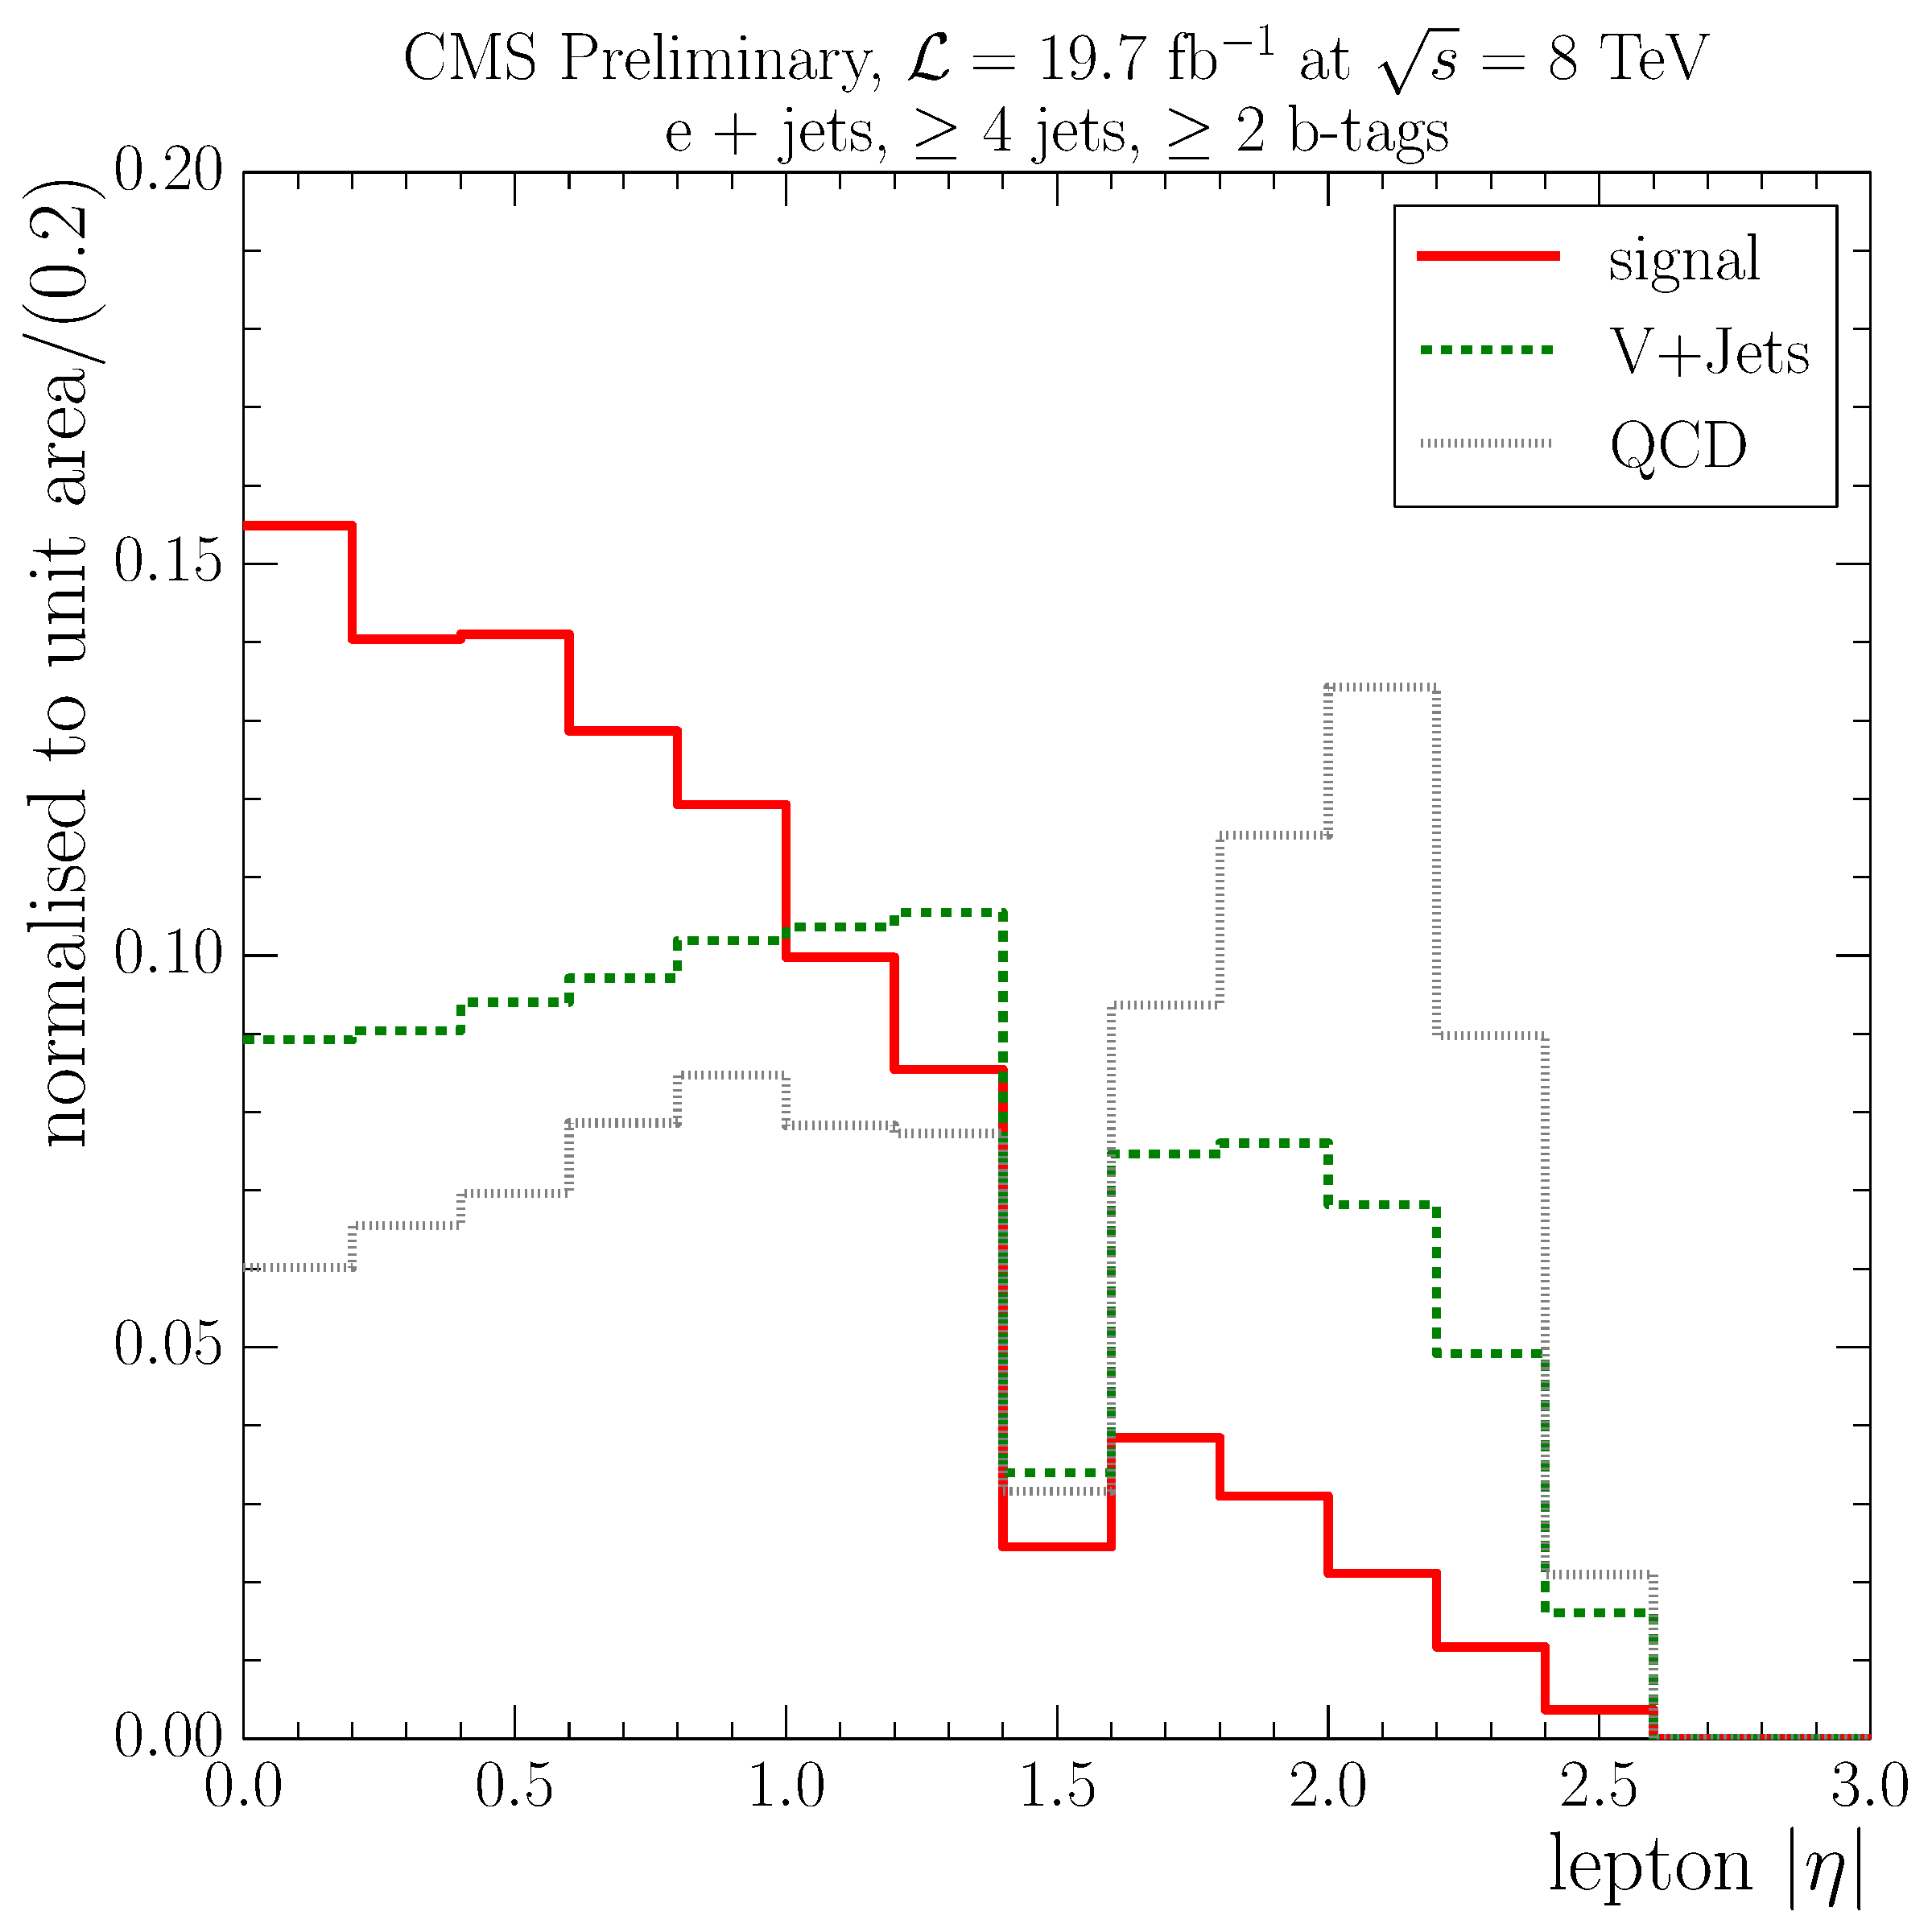
\includegraphics[width=0.39\textwidth]{measurement/WPT/central/fit_templates/electron_templates_bin_0-40}}\hfill
    {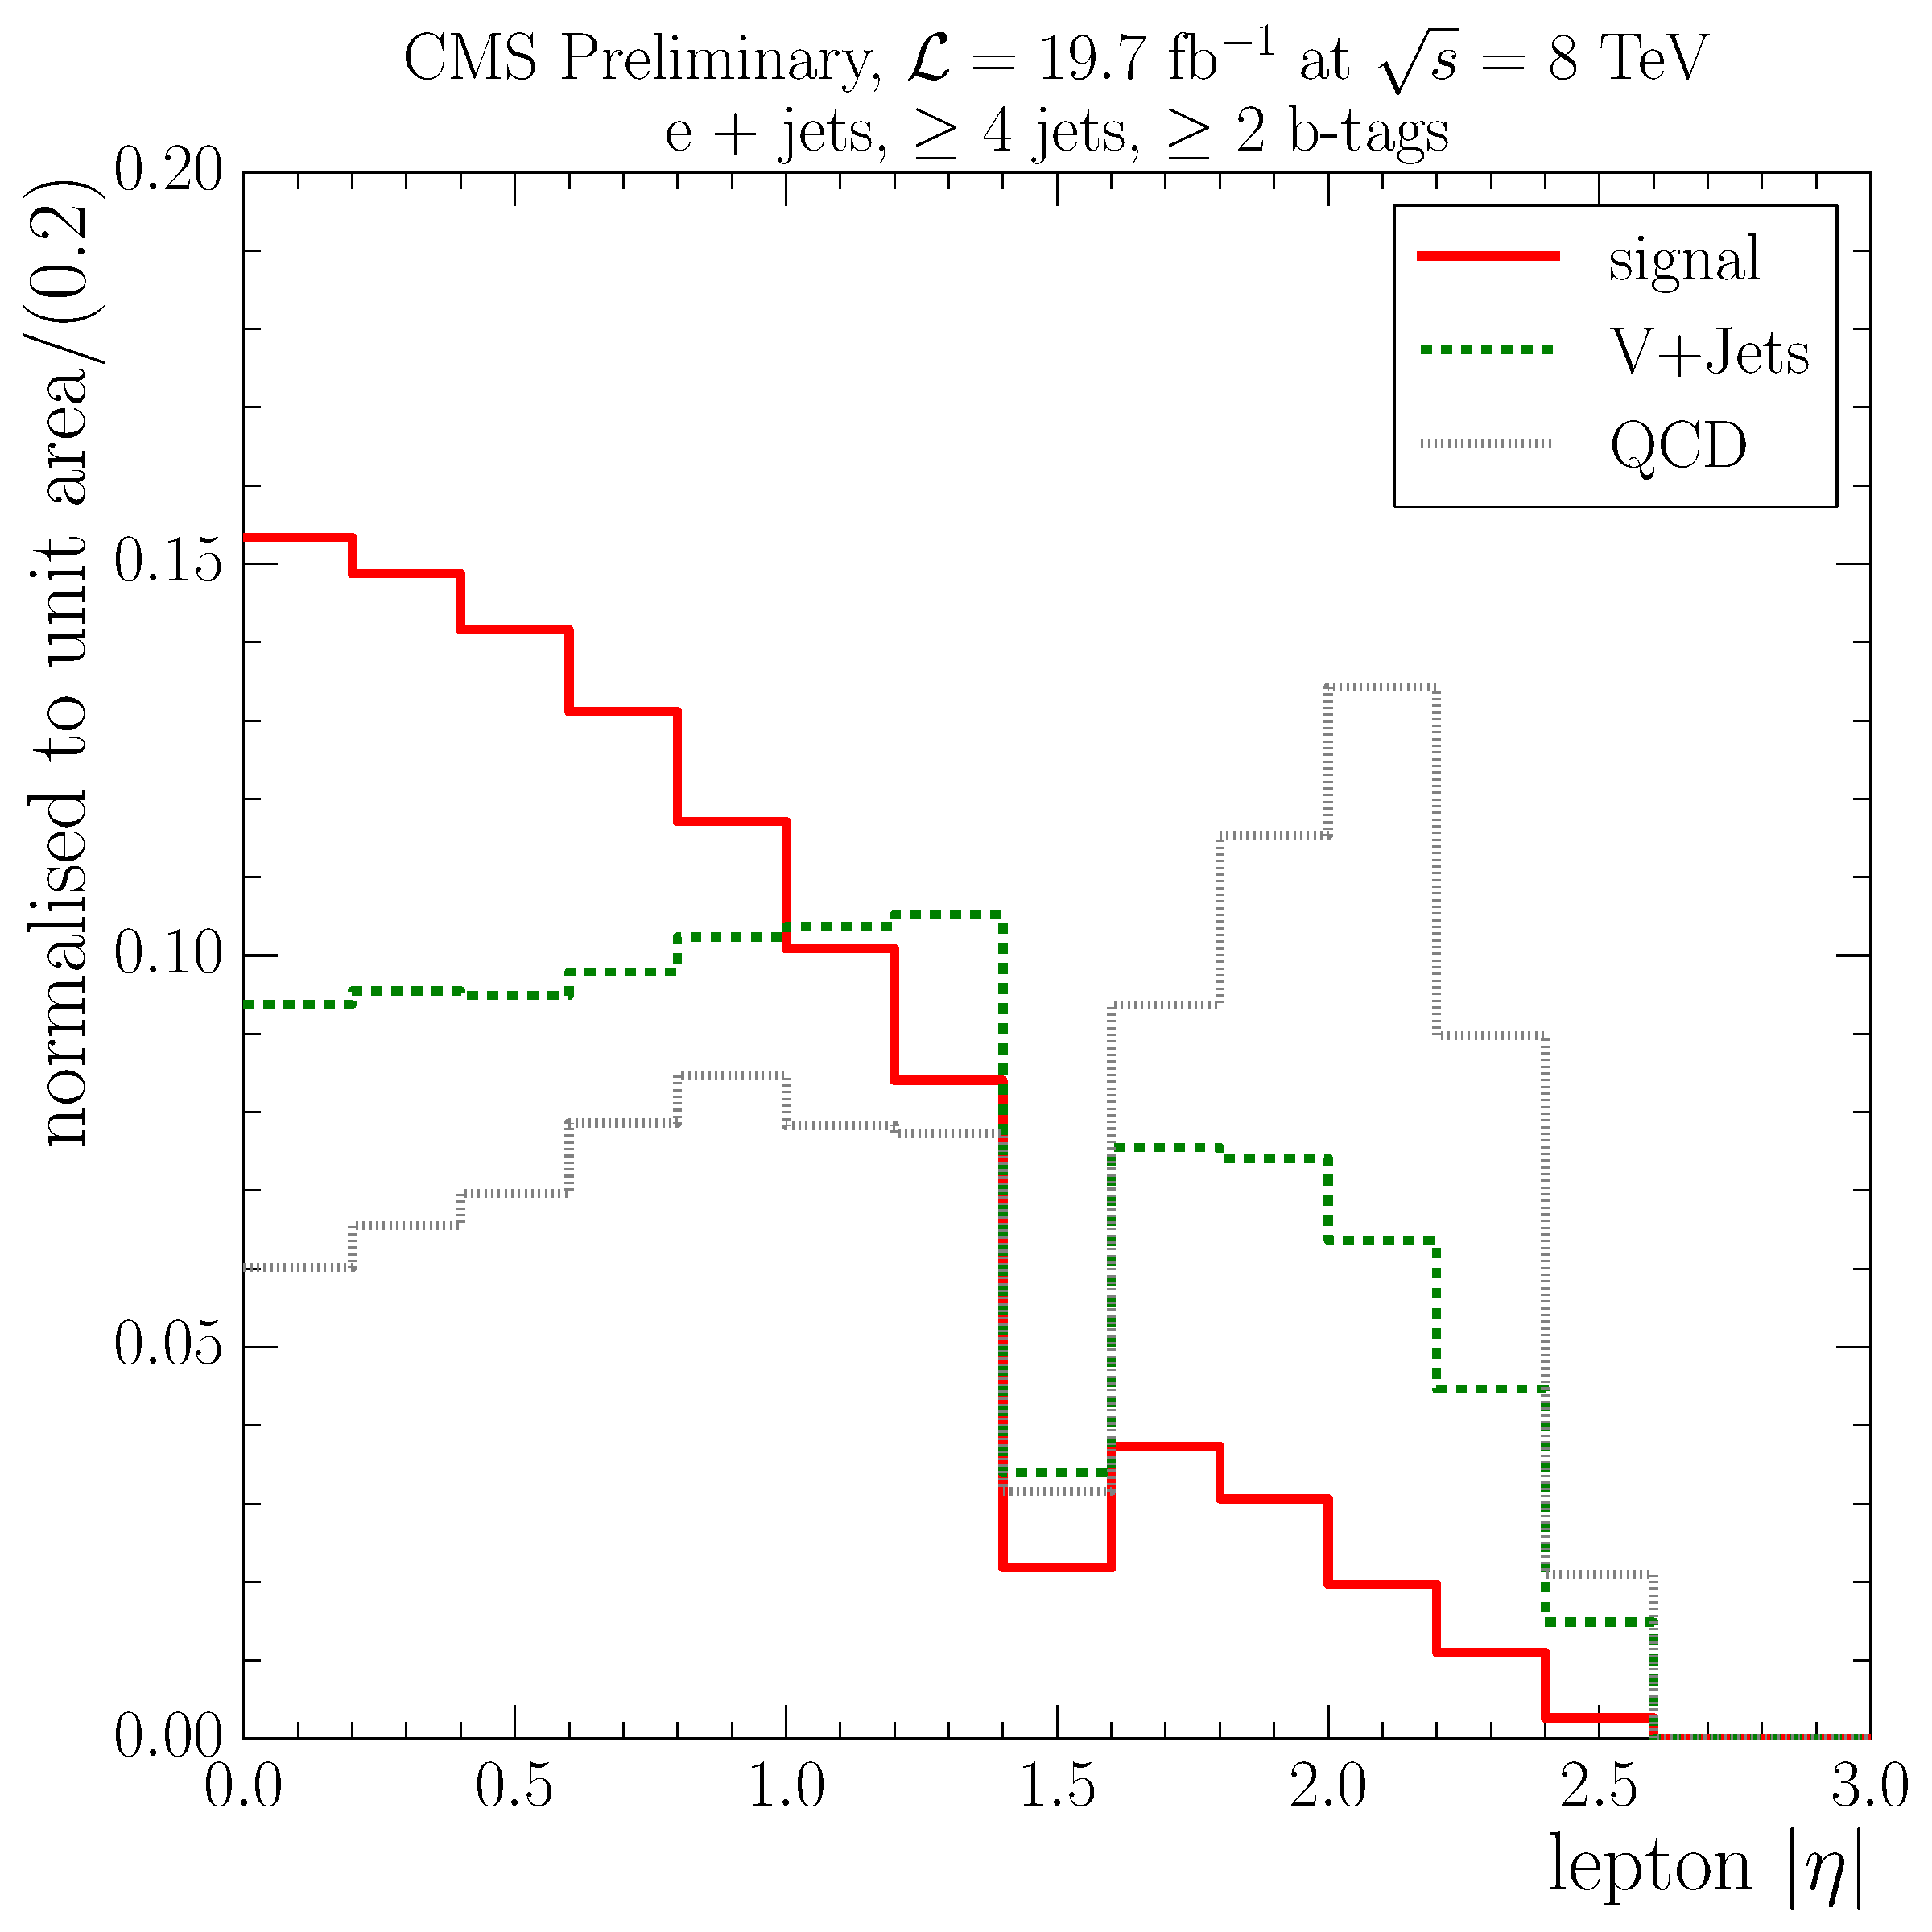
\includegraphics[width=0.39\textwidth]{measurement/WPT/central/fit_templates/electron_templates_bin_40-70}}
    \hspace*{\fill} \\
    \hspace*{\fill}
    {\includegraphics[width=0.39\textwidth]{measurement/WPT/central/fit_templates/electron_templates_bin_70-100}}\hfill
    {\includegraphics[width=0.39\textwidth]{measurement/WPT/central/fit_templates/electron_templates_bin_100-130}}
    \hspace*{\fill} \\
    \hspace*{\fill}
    {\includegraphics[width=0.39\textwidth]{measurement/WPT/central/fit_templates/electron_templates_bin_130-170}}\hfill
    {\includegraphics[width=0.39\textwidth]{measurement/WPT/central/fit_templates/electron_templates_bin_170-inf}}
    \hspace*{\fill}
    \caption{Electron $\abs \eta$ templates for the fit in different bins of \WPT,
    from top left to bottom right: \SIrange{0}{40}{\GeV}, \SIrange{40}{70}{\GeV},
    \SIrange{70}{100}{\GeV}, \SIrange{100}{130}{\GeV}, \SIrange{130}{170}{\GeV} and $\geq \SI{170}{\GeV}$.}
    \label{fig:fit_tempaltes_WPT_electron}
\end{figure}

\begin{figure}[!htbp]
  \centering
    \hspace*{\fill}
    {\includegraphics[width=0.39\textwidth]{measurement/WPT/central/fit_templates/muon_templates_bin_0-40}}\hfill
    {\includegraphics[width=0.39\textwidth]{measurement/WPT/central/fit_templates/muon_templates_bin_40-70}}
    \hspace*{\fill} \\
    \hspace*{\fill}
    {\includegraphics[width=0.39\textwidth]{measurement/WPT/central/fit_templates/muon_templates_bin_70-100}}\hfill
    {\includegraphics[width=0.39\textwidth]{measurement/WPT/central/fit_templates/muon_templates_bin_100-130}}
    \hspace*{\fill} \\
    \hspace*{\fill}
    {\includegraphics[width=0.39\textwidth]{measurement/WPT/central/fit_templates/muon_templates_bin_130-170}}\hfill
    {\includegraphics[width=0.39\textwidth]{measurement/WPT/central/fit_templates/muon_templates_bin_170-inf}}
    \hspace*{\fill}
    \caption{Muon $\abs \eta$ templates for the fit in different bins of \WPT,
    from top left to bottom right: \SIrange{0}{40}{\GeV}, \SIrange{40}{70}{\GeV},
    \SIrange{70}{100}{\GeV}, \SIrange{100}{130}{\GeV}, \SIrange{130}{170}{\GeV} and $\geq \SI{170}{\GeV}$.}
    \label{fig:fit_templates_WPT_muon}
\end{figure}


\newpage
\section*{\MT variable}

\begin{figure}[!htbp]
  \centering
    \hspace*{\fill}
    {\includegraphics[width=0.39\textwidth]{measurement/MT/central/fit_templates/electron_templates_bin_0-30}}\hfill
    {\includegraphics[width=0.39\textwidth]{measurement/MT/central/fit_templates/electron_templates_bin_30-50}}
    \hspace*{\fill} \\
    \hspace*{\fill}
    {\includegraphics[width=0.39\textwidth]{measurement/MT/central/fit_templates/electron_templates_bin_50-80}}\hfill
    {\includegraphics[width=0.39\textwidth]{measurement/MT/central/fit_templates/electron_templates_bin_80-100}}
    \hspace*{\fill} \\
    \hspace*{\fill}
    {\includegraphics[width=0.39\textwidth]{measurement/MT/central/fit_templates/electron_templates_bin_100-inf}}
    \hspace*{\fill}
    \caption{Electron $\abs \eta$ templates for the fit in different bins of \MT,
    from top left to bottom right: \SIrange{0}{30}{\GeV}, \SIrange{30}{50}{\GeV},
    \SIrange{50}{80}{\GeV}, \SIrange{80}{100}{\GeV} and $\geq \SI{100}{\GeV}$.}
    \label{fig:fit_tempaltes_MT_electron}
\end{figure}

\begin{figure}[!htbp]
  \centering
    \hspace*{\fill}
    {\includegraphics[width=0.39\textwidth]{measurement/MT/central/fit_templates/muon_templates_bin_0-30}}\hfill
    {\includegraphics[width=0.39\textwidth]{measurement/MT/central/fit_templates/muon_templates_bin_30-50}}
    \hspace*{\fill} \\
    \hspace*{\fill}
    {\includegraphics[width=0.39\textwidth]{measurement/MT/central/fit_templates/muon_templates_bin_50-80}}\hfill
    {\includegraphics[width=0.39\textwidth]{measurement/MT/central/fit_templates/muon_templates_bin_80-100}}
    \hspace*{\fill} \\
    \hspace*{\fill}
    {\includegraphics[width=0.39\textwidth]{measurement/MT/central/fit_templates/muon_templates_bin_100-inf}}
    \hspace*{\fill}
    \caption{Muon $\abs \eta$ templates for the fit in different bins of \MT,
    from top left to bottom right: \SIrange{0}{30}{\GeV}, \SIrange{30}{50}{\GeV},
    \SIrange{50}{80}{\GeV}, \SIrange{80}{100}{\GeV} and $\geq \SI{100}{\GeV}$.}
    \label{fig:fit_templates_MT_muon}
\end{figure}

\sisetup{range-phrase = {~to~}}
\sisetup{range-units = repeat}

%%% Local Variables: 
%%% mode: latex
%%% TeX-master: "../thesis"
%%% End: 
